\documentclass[11pt,a4paper]{report}
%\documentclass[11pt,a4paper,twoside,openright]{report}

\usepackage[utf8]{inputenc}
\usepackage{ragged2e}
\usepackage{amsmath}
\usepackage{amssymb}
\usepackage{makecell}

%\usepackage[meec]{feupteses}
%\usepackage[meec,juri]{feupteses}
\usepackage[meec,final]{feupteses}

\graphicspath{{figures/}}

\addbibresource{bibliography.bib}

\begin{document}

\title{Characterization of Retinal Fluid in OCT Images}
\author{David Castanho Terroso}

\thesisdate{July 22, 2025}

\copyrightnotice{David Castanho Terroso, 2025}

\supervisor{Supervisor}{Prof.\ Tânia Melo}
\supervisor{Co-Supervisor}{Prof.\ Ana Maria Mendonça}

%\committeetext{Approved in oral examination by the committee:}
%\committeemember{President}{Prof.\ José Machado da Silva}
%\committeemember{Referee}{PhD.\ Filipe Soares}

%\signature

\logo{uporto-feup.pdf}

\begin{Prolog}
  \chapter*{Resumo}

\chapter*{Abstract}
Damage to the retina can result in significant visual impairment, negatively limiting the quality of life of those impacted. Diseases such as age-related macular degeneration (AMD), diabetic macular edema (DME), and retinal vein occlusion (RVO) are among the leading causes of retinal damage and are typically characterized by the presence and accumulation of fluid in the retina. 
\par
The characteristics of these fluids, visible in retinal optical coherence tomography (OCT) scans, serve as important biomarkers in disease progression. However, the manual annotation of these fluids is laborious, time consuming, and prone to inter-observer variability, which motivates the need for automatic characterization approaches.
\par
This dissertation explores the state-of-the-art deep learning techniques for semantic segmentation of retinal fluids, targeting the segmentation of intra-retinal fluid (IRF), sub-retinal fluid (SRF), and pigment epithelial detachment (PED), in the RETOUCH dataset. 
\par
Additionally, the work investigates the use of generative models, such as the generative adversarial networks (GANs), to synthesize intermediate OCT slices, aiming to enhance the inter-slice resolution throughout an OCT volume. The segmentation results in the enhanced dataset are used in the fluid volume calculation, an important biomarker in the progression of the mentioned retinal diseases.
\par
The experimental works show that the segmentation model achieved comparable outcomes with the existing approaches in the literature, particularly when using as input larger patches that contribute with enough anatomic context for the segmentation. Meanwhile, the generative models, though less explored in OCT, demonstrate promising results in the synthesis of realistic interpolated slices. This combination of segmentation and generation supports a more robust characterization of the retinal fluids, providing more confidence to the fluid volumes estimated.
\par
Despite the encouraging obtained results, several limitations remain, particularly in segmentation model generalization to external datasets and in the fine-detail realism of the generated slices and segmentation masks. Future works should explore advanced architectures, such as attention mechanism, and perceptual loss functions, to improve detail and robustness across diverse imaging conditions.
  \chapter*{UN Sustainable Development Goals} \label{chap:UnitedNations}

The United Nations Sustainable Development Goals (SDGs) provide a global framework to achieve a more equitable, healthy, and sustainable future for all. Comprising 17 different goals, this framework addresses pressing world's challenges, including poverty, hunger, health, and education.
\par
This dissertation contributes to these SDGs by advancing automated tools for the detection and characterization of retinal diseases, which are among the leading causes of vision impairment and blindness. The proposed methods support the ``SDG 3: Ensure healthy lives and promote well-being for all at all ages'', by developing fast, automatic, scalable, and accurate diagnostic tools that assist in the early identification and monitoring of retinal conditions. Since these solutions are fast, accessible, and easily deployed, they have the potential to be used in developing countries, where resources and access to trained specialists are scarce, supporting Target 3.d., which aims to support the capacity of all countries for early detection and monitoring of health risks. Additionally, through the prediction and monitoring of retinal diseases, this technology can also reduce the load on the healthcare systems, while improving decision-making and access to more equitable healthcare, once again addressing Target 3.d.
\par
In addition to the healthcare contributions, the studied technology can also be implemented as a educational material, providing an alternative tool for the understanding and visualization of retinal fluid pathologies, aligning with ``SDG 4: Ensure inclusive and equitable quality education and promote lifelong learning opportunities for all''. This addresses Target 4.4, which focuses on increasing of the number of young adults with relevant technical skills, and Target 3.c, which aims to improve the training of healthcare personnel.
\par
The relevant SGDs, their associated contributions, and performance metrics are explained in the following table:

\begin{description}
\item [SDG 3]
Ensure healthy lives and promote well-being for all at all ages
\item [SDG 4]
Ensure inclusive and equitable quality education and promote lifelong learning opportunities for all
\end{description}

\begin{center}
	\begin{tabular}{|l|l|p{58mm}|p{52mm}|}
		\hline
		\textbf{SGD} & \textbf{Target} & \textbf{Contribution} & \textbf{Performance Indicators and Metrics} \\ 
		\hline
		\hline
		\multirow{3}{*}{3} 
		& 3.d & Developed a GAN that generates intermediate slices between two known scans, increasing the spatial resolution and continuity of OCT volumes. & Reduction in misdiagnosis cases; Increased detection of early-stage retinal conditions.\\
		\cline{2-4}
		& 3.d & Designed an automatic fluid volume estimation pipeline that integrates retinal fluid segmentation and slice generation, and can accurately calculate the quantity of each fluid in type (IRF, SRF, and PED) an OCT volume, enabling disease progression monitoring and reducing clinician workload. & Reduction in clinician time spent per patient; Improved diagnostic consistency across clinicians.\\
		\cline{2-4}
		& 3.c & \parbox[t]{58mm}{Developed a segmentation model that performs accurate retinal fluid segmentation in OCT B-scans automatically, and can be used as an educational tool for understanding of retinal pathologies.} & \parbox[t]{52mm}{Improvement in diagnostic skills before and after using this tool; Increased acceptability of AI tools in the clinical workflow.}\\
		\cline{1-2}
		4 & 4.4 & & \\
		\hline
	\end{tabular}
\end{center}
  \chapter*{Acknowledgements}
%\addcontentsline{toc}{chapter}{Acknowledgements}

As this dissertation marks the end of my studies, it is of my responsibility to thank and acknowledge all of those who shaped the path that lead me here.
\par
First, I would like to thank my supervisor Prof. Tânia Melo and my co-supervisor Prof. Ana Maria Mendonça for all the support, dedication, and patience throughout this dissertation. They motivated me to dig deeper in the topics here approached, inspiring me and forging my knowledge, while sharing their experienced and useful insights.
\par
As I thank my supervisors, I must also thank all the professors that motivated, inspired, and, most importantly, taught me along my academic path. From English to equations and programming, the knowledge transmitted by them fills the pages of this document.
\par
I am also grateful for all the friends that made part of this process. Therefore, I thank those that I met at FEUP and made the experience in this university more fun and enjoyable. The burdens shared with them will never be forgotten, as they made the ride of the last two years smoother. I also thank those that have accompanied me since high school, who showed me the corners of this university and shared their technical insights in the topics approached in this dissertation, despite sharing a different background. It has been a pleasure to watch you grow beside me.
\par
I can not write the acknowledgments without thanking my family, especially my parents and my sister Sofia, who have been supporting me all the way through the academic path that lead me to this master's. No dissertation could have been done without your unconditional support, even when you had no clue what I was writing about.
\par
Lastly, I have to thank Mariana for all the support and companionship she provided during this journey. Especially in the last weeks, where the pressure and uncertainty started to accumulate, she made sure I kept going and gracefully completed this document. Without you, this dissertation would never happened, as you continuously encouraged me to pursuit it, believing in me more than I did. For that faith, I thank you. The growth I have experienced in these last weeks, months, and years are a reflection of your motivation to keep going and chasing my dreams, pushing me to make the most out of my capabilities. Sharing this journey and helping you whenever I could were some of the best moments I have ever lived, I am very delighted to see you succeed by my side. Without a doubt, the best and most important part of this path.

\vspace{10mm}
\flushleft{David Castanho Terroso}

  %% This section is optional and can be removed
\cleardoublepage
\thispagestyle{plain}

\vspace*{8cm}

\begin{flushright}
   \textsl{``Our greatest glory is not in never falling, but in rising every time we fall''} \\
\vspace*{1.5cm}
    Confucius
\end{flushright}

  \cleardoublepage
  
  \pdfbookmark[0]{Table of Contents}{contents}
  \tableofcontents
  \cleardoublepage
  \pdfbookmark[0]{List of Figures}{figures}
  \listoffigures
  \cleardoublepage
  \pdfbookmark[0]{List of Tables}{tables}
  \listoftables
  \chapter*{List of Acronyms}
\chaptermark{LIST OF ACRONYMS}

\begin{flushleft}
\begin{tabular}{l p{0.8\linewidth}}
	
AMD      & Age-related macular degeneration\\
AMI 	 & Anisotropic meta interpolation\\
BCE		 & Binary cross-entropy\\
BM   	 & Brunch's membrane\\
CDFI 	 & Compression-driven network design for frame interpolation\\
CHUSJ 	 & Centro Hospitalar Universitário de São João\\
CNN      & Convolutional neural network\\
CS 		 & Contrast sensitivity\\
CT 		 & Computed tomography\\
DME      & Diabetic macular edema\\
GAN 	 & Generative adversarial network\\
GDL 	 & Gradient difference loss\\
GT  	 & Ground truth\\
HR 		 & High-resolution\\
ILM 	 & Internal limiting membrane\\
IRF      & Intraretinal fluid\\
MAE 	 & Mean absolute error\\
MRI 	 & Magnetic resonance imaging\\
MSE		 & Mean square error\\	
MS-SSIM  & Multi-scale structural similarity index measure\\
LR 		 & Low-resolution\\
OCT      & Optical coherence tomography\\
ONL      & Outer nuclear layer\\
PED      & Pigment epithelial detachment\\
PSNR 	 & Peak signal-to-noise ratio\\
RIFE	 & Real-time interpolation flow estimation\\
RGB 	 & Red, green, and blue\\
ROI		 & Region of interest\\
RPE      & Retinal pigment epithelium\\
RVO 	 & Retinal vein occlusion\\
SR		 & Super-resolution\\
SRF      & Subretinal fluid\\
SSIM 	 & Structural similarity index measure\\
\end{tabular}
\end{flushleft}


\end{Prolog}

\StartBody

\chapter{Introduction}
The vision is the human's most important and complex sense, playing a critical role in our orientation in the world \parencite{Hutmacher2019}. However, the health of the retina, an important part of the eye, can be compromised by multiple diseases, that lead to fluid accumulation in it. The characterization of the fluid present in the retina is important to assess the progression of diseases such as age-related macular degeneration (AMD), diabetic macular edema (DME), and macular edema secondary to retinal vein occlusion (RVO) \parencite{Bogunovic2019a}.
\par
AMD affects the macular region of the retina, leading, in later stages, to a significant and permanent loss of central visual acuity, which has a severe impact on the patient's quality of life. In patients with AMD, the formation of new blood vessels can occur, which leak fluid, lipids, and blood into the retina, resulting in the formation of retinal fluid \parencite{Lim2012}. It is one of the leading causes of visual impairment with an expected effect on 300 million people by 2040 \parencite{Mitchell2018}.
\par
In patients with diabetes mellitus, DME represents the most common cause of visual impairment, affecting approximately 150 million people worldwide, as of 2015. It is anticipated that this number will increase as the prevalence of diabetes in developed countries is growing \parencite{Musat2015}. The fluid accumulation is caused by a disruption of the blood-retinal barrier, which allows fluid to accumulate in the intraretinal layers of the macula, resulting in retinal thickening (edema) \parencite{Bhagat2009, Bandello2019}.
\par
Affecting 16 million people worldwide, RVO represents a significant cause of vision loss in older individuals. The occlusion of the retinal vein can result in swelling of the optic disc, which leads to a reduction in visual acuity \parencite{Wong2010}. 
\par
The presence of intraretinal fluid (IRF) is a defining criterion of DME and RVO, while two in every three patients with AMD present this type of fluid. The majority of patients with AMD and 30\% of the patients with DME and RVO have subretinal fluid (SRF). Pigment epithelial detachments (PED) occurs more frequently in patients with AMD \parencite{Bogunovic2019a}.
\par
Therefore, retinal fluids are important for the classification and progression of these diseases, and can be observed through retinal optical coherence tomography (OCT) \parencite{Bogunovic2019a}. OCT is a non-invasive imaging technique that analyzes the light behavior (such as its reflection, absorption, and time-of-flight) to estimate the spatial dimensions of the tissue's structure \parencite{Huang1991}. This allows for \textit{in vivo} visualization of the individual retinal layers within the posterior segment of the eye. An OCT is composed of multiple consecutive cross-sectional 2D images that, when stacked, form a volumetric representation of the posterior segment. Each of these two-dimensional images is referred to as B-scans and an example can be seen in Figure \ref{fig:SegmentedFluidsOCT}. The resolution is sufficiently high to assess the tissue integrity, the retinal layers, and the fluids present \parencite{Drexler2008, Viedma2022}. There are multiple devices used for the acquisition of OCT volumes, resulting in different image attributes across the same technique, such as interslice distance, image quality, and appearance \parencite{Bogunovic2019a}. 
\par
The classification of the fluid is dependent on its location within the retina. There are three different categories: IRF, which is situated in the inner and outer layers of the retina; SRF, positioned between the outer nuclear layer (ONL) and the retinal pigment epithelium (RPE); and PED, which appear beneath the RPE \parencite{Bogunovic2019a}. Figure \ref{fig:SegmentedFluidsOCT} shows the characteristics and positions of these fluids on an OCT B-scan and Figure \ref{fig:RetinalLayers} exhibits the retinal layers in the OCT scan of a healthy patient.
\par
\begin{figure}[!ht]
	\centering
	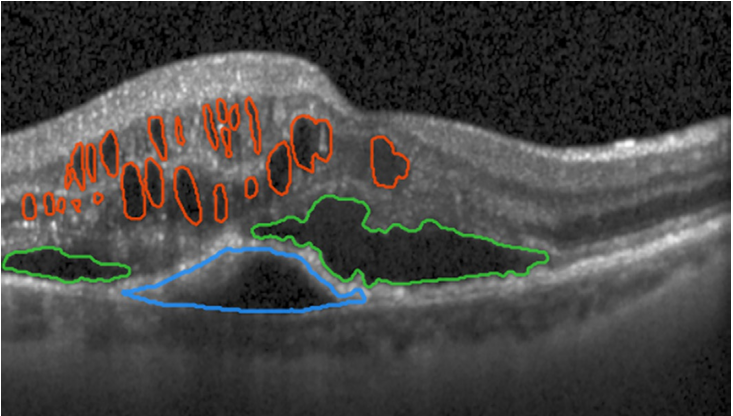
\includegraphics[width=0.75\linewidth]{../figures/SegmentedFluidsOCT.png}
	\caption{The three distinct fluid types on an OCT B-scan: IRF in red, SRF in green, and PED in blue \cite{Bogunovic2019a}.}
	\label{fig:SegmentedFluidsOCT}
\end{figure}
\begin{figure}[!ht]
	\centering
	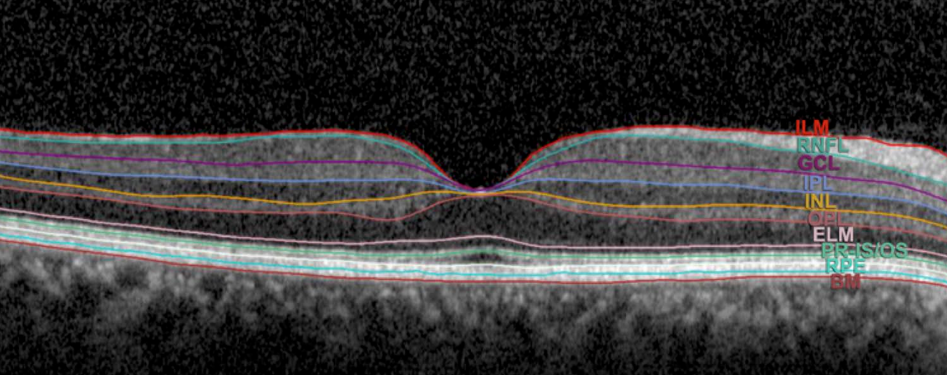
\includegraphics[width=1\linewidth]{../figures/RetinalLayers}
	\caption{OCT scan of the retinal layers \cite{Almonte2020}.}
	\label{fig:RetinalLayers}
	\footnotesize
	\justifying
	BM, Bruch's membrane; ELM, external limiting membrane; GCL, ganglion cell layer; ILM, internal limiting membrane; INL, inner nuclear layer; IPL, inner plexiform layer; ONL, outer nuclear layer; OPL, outer plexiform layer; PR-IS/OS, photoreceptor inner segment/outer segment; RNFL, retinal nerve fibre layer; RPE, retinal pigment epithelium.
\end{figure}
\par
By segmenting the fluids detected in the B-scans, their volume can be estimated and used as a progression marker of the mentioned retinal diseases. However, manual segmentation is laborious, expensive, and prone to bias, which motivates the search for automatic methods \cite{Viedma2022}. 
\par
In OCT imaging, the precision of the estimated volume is not only dependent on the quality of the segmentation, but also on the interslice distance \cite{Lopez2023}. It is seen in other imaging techniques that the performance of the segmentation is improved when the neighboring slices are used as input. Consequently, the reduction in interslice distance and improvement of the resolution along this axis, betters the performance of models that include information from adjacent slices \cite{Selvi2013}. Given that the interslice space is reduced, the estimated segmented volume will also be closer to the real fluid volume.
\par
Considering the previous statements, the dissertation general objective is to conduct an analysis of retinal OCT scans, classifying the retinal fluids in three distinct types (IRF, SRF, and PED) and quantifying their respective volumes. Another important objective is to increase the interslice resolution of the OCT volumes, with the aim of improving the fluid volume estimation. The specific objectives were determined as follows:  
\begin{enumerate}
	\item Develop different 2D deep learning models for multi-class segmentation of retinal fluids (IRF, SRF, and PED) in OCT volumes.
	\item Compare the best performing 2D model with a previously implemented 2.5D model.
	\item Evaluate the performance of the best segmentation model and estimate the volume of each fluid using the masks predicted by it.
	\item Use of a generative model for synthesizing intermediate slices in OCT volumes, generating one or more slices between two real slices to improve the interslice resolution of the volume, while assessing the quality of these generated images.
	\item Investigate the impact of intermediate slices synthesis on the fluid volume estimation by the segmentation models. 
\end{enumerate}
\par
Apart from the ``Introduction'', the dissertation is composed of the following chapters: ``Literature Review'', ``Methods'', ``Results'', ``Discussion'', and ``Conclusion''. In the ``Literature Review'' chapter, an analysis is performed on the latest papers in the field of retinal fluid segmentation using 2D deep learning networks, as well as the latest publications on interslice resolution enhancement. The ``Methods'' chapter details the selection of the dataset for the experiments performed during the dissertation, alongside with an insightful description of the experiments. In the ``Results'' chapter, the results from each experiment are shared, showing the performance of each model in their respective task, while the ``Discussion'' chapter explains the performance differences between experiments, comparing them to the literature. Finally, the ``Conclusion'' shows the main findings from the experiments performed and suggests directions of further research.
 
\chapter{Literature Review}\label{LiteratureReview}
For this dissertation, research was conducted to identify the most recent trends in 2D fluid segmentation of OCT volumes using deep learning, as well as the application of generative models for intermediate slice synthesis.
\section{Fluid Segmentation in OCT Scans}
In the fluid segmentation state-of-the-art research, articles were retrieved using a systematic review methodology. The next subsection details the retrieval process and the criteria for inclusion and exclusion of the articles. Section \ref{FluidSegmentationLiteratureReview} presents the trends in methodologies used for fluid segmentation.
\subsection{Search Strategy}\label{SearchStrategy}
The search query was defined as: ````OCT'' AND ``segmentation'' AND (``deep learning'' OR ``CNN'' OR ``neural network'')''. Using the query, papers were retrieved from four different databases: 398 articles from PubMed, 105 from IEEE, 125 from ScienceDirect, and 80 from ACM.
\par
In the process of collecting the papers, those published over the previous five years and regarding 2D or 2.5D fluid segmentation in OCT volumes were included. Additionally, conference proceedings, non-English articles, and articles without the full text accessible were excluded.
\par
A total of 708 articles were initially identified, of which 133 were duplicates. Afterwards, 575 articles were screened, based on titles and abstracts. These articles were analyzed in accordance with the inclusion and exclusion criteria, resulting in the removal of 499 papers. Of the remaining 76 articles for the full-text screening, 20 met the established criteria. These final articles represent the state-of-the-art in 2D deep learning-based fluid segmentation in OCT volumes included and form the foundation of the literature reviewed in this dissertation.

\subsection{Trends in Segmentation Methodologies}\label{FluidSegmentationLiteratureReview}
The selected papers can be divided into two broad groups, according to the type of segmentation: binary segmentation \parencite{Quek2022, Pawan2021, Liu2021, Guo2020, Wang2021, Wu2023}, where the fluid is classified in one whole class, and multi-class segmentation \parencite{Rahil2023, Hassan2021a, Zhang2023, Sappa2021, Xing2022, Tang2022, Padilla2022, Hu2019, Mantel2021, Liu2024, Li2023, Gao2019, Hassan2021b, Lu2019}, where the segmented fluid is classified in two or more classes (namely IRF, SRF, and PED). Additional grouping criteria include the segmentation architecture and the use of retinal delimitation, as shown in Figure \ref{fig:ArticlesSelection}.
\par
In binary segmentation, the approaches to the segmentation problem are simpler, but include both convolutional neural networks (CNN) \parencite{Pawan2021, Liu2021, Guo2020, Wang2021, Wu2023} and transformer solutions \parencite{Quek2022}. The CNN solutions differ among them, depending on the modules that constitute each network, but all are inspired by the U-Net \parencite{Ronneberger2015}. In Figure \ref{fig:BinarySegmentationExample}, an instance of a CNN used for binary fluid segmentation is shown.
\begin{figure}[!ht]
	\centering
	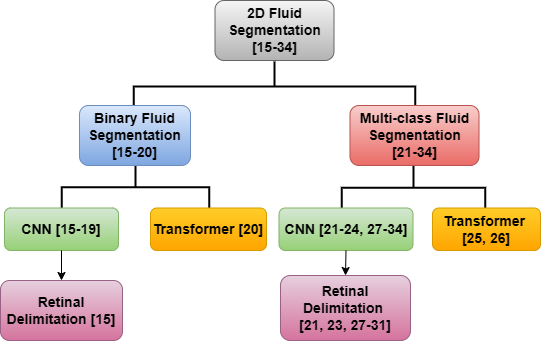
\includegraphics[width=0.75\linewidth]{figures/ArticlesSelection.png}
	\caption{Grouping of the articles included in the literature review.}
	\label{fig:ArticlesSelection}
\end{figure}
\begin{figure}[!ht]
	\centering
	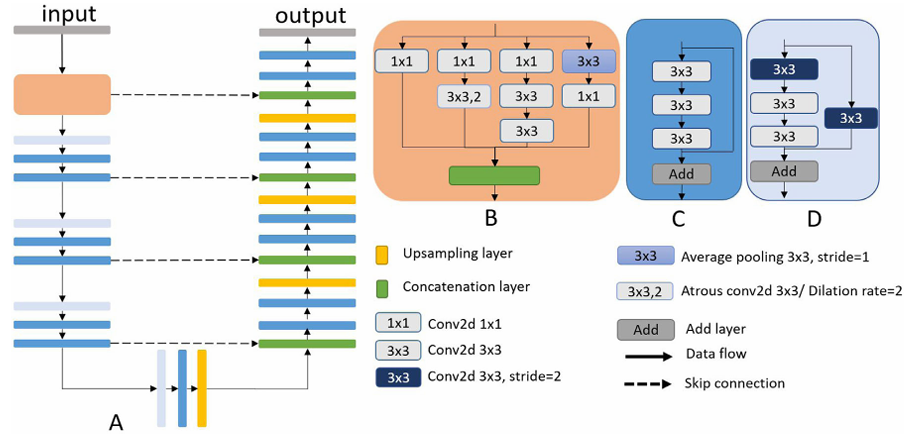
\includegraphics[width=1\linewidth]{figures/BinarySegmentationExample.png}
	\caption{Example of a CNN architecture used for binary fluid segmentation. Image A depicts the neural network architecture, B shows the used multi-scale block, while C and D exhibit the residual convolutional blocks \parencite{Guo2020}.}
	\label{fig:BinarySegmentationExample}
\end{figure}
\par
The work of \textcite{Pawan2021} is the only one in binary segmentation that restricts the input of the CNN to the content within the retinal layer. This approach is frequently observed in the papers focused on multi-class segmentation. In \parencite{Pawan2021}, this is achieved by performing a retinal layer segmentation and assigning all the values outside the boundaries to zero. The result of this operation serves as input to the CNN. The removal of irrelevant information surrounding the retina simplifies the learning process and improves the model's focus on essential information \parencite{Mantel2021}.
\par
In the framework proposed by \textcite{Liu2021}, the  slice's fluid mask and distance map are generated. The distance map consists of the predicted distance of each pixel to the retinal tissue, with only the values above a specified distance threshold being kept. This is achieved through the use of a double-branched network, where the encoder is the same, while the decoders vary. One decoder is responsible for generating the fluid segmentation map, while the other predicts the distance map. This distance map is then converted to a binary mask by applying a threshold value: pixels with greater distance than this value are set to one, and all others to zero. The intersection between the fluid segmentation map and this binary mask forms the final segmentation. This approach mitigates the issue of inappropriate merging of small and proximate fluid regions, as the distance map branch is better than the fluid segmentation network in discerning the boundaries that delineate fluid regions.
\par
Resorting to generative adversarial networks (GANs), \textcite{Wu2023} make images from different vendors visually similar to the images of a singular, specific vendor. Subsequently, a U-Net, which has extensively been trained on images from that specific vendor, is used for segmentation. This approach is intended to reduce the burden of learning the segmentation on multiple vendors by ensuring that all volumes are similar to one in which the segmentation model performs well. The multi-class segmentation framework proposed by \textcite{Li2023} was designed based on the same idea. 
\par
CNNs inspired by the U-Net can also be combined with transformers in the context of binary fluid segmentation \parencite{Quek2022}. While CNNs capture the information from local receptive fields, visual transformers integrate features from global receptive fields. In the neural network proposed by \textcite{Quek2022}, the visual transformers are located between the encoder and decoder paths, thus incorporating features from both receptive fields in the encoding branch.
\par
The majority of the papers included in this review perform multi-class segmentation, which results in a broader range of implementation strategies. While all of them segment two or more types of fluids, \textcite{Hassan2021a} and \textcite{Padilla2022} also segment other retinal biomarkers. Similarly to binary segmentation, the multi-class segmentation papers can also be divided according to the presence \parencite{Zhang2023, Liu2024} or absence \parencite{Rahil2023, Hassan2021a, Sappa2021, Xing2022, Tang2022, Padilla2022, Hu2019, Mantel2021, Li2023, Gao2019, Hassan2021b, Lu2019} of transformers in the segmentation network. All the papers that have transformers in their framework combine them with CNNs. 
\par
Similar to what was developed by \textcite{Quek2022}, \textcite{Liu2024} have integrated transformers in the bottleneck section of a segmentation network inspired by the U-Net. The authors utilize two networks for the segmentation: one for coarse segmentation and other for the refinement of the results from the first. Both networks are similar to the U-Net, but a transformer is included in the refinement branch. Its purpose is to provide features from global fields, compensating for the deep features that are used as input in this branch. In contrast, \textcite{Zhang2023} replaced the CNN encoder with a transformer encoder, exploiting its modeling capacity with self-attention.
\par
The limitation of the input to the region within the retinal layer, ignoring what is outside of it, is seen in many of the multi-class papers \parencite{Hassan2021b, Hassan2021a, Lu2019, Mantel2021, Rahil2023, Tang2022, Xing2022}, similarly to what was done in \textcite{Pawan2021}. There are various approaches for this delimitation, with some using CNNs trained for the segmentation of the retinal layers or the retina \parencite{Mantel2021, Tang2022}, and others relying on algorithms that detect the distinct transition in intensity or texture between the retina and the surrounding tissue or background \parencite{Hassan2021b, Hassan2021a, Lu2019, Rahil2023, Xing2022, Pawan2021}. 
\par
The retinal delimitation is conducted as a separate process from the fluid segmentation. In \parencite{Tang2022, Hassan2021b, Hassan2021a, Lu2019, Rahil2023, Xing2022}, the retinal layer is segmented prior to the fluid segmentation, conditioning the input of the fluid segmentation network and simplifying the learning process. However, the retinal delimitation can also constrain the final output by limiting segmentation to the retinal layer zone, as observed in \textcite{Mantel2021}.
\par
The input can be conditioned in multiple ways. \textcite{Xing2022} crop the image to fit the region of interest. In \parencite{Rahil2023, Tang2022, Lu2019}, the OCT B-scan is combined with the retinal delimitation result through concatenation. Conversely, in \parencite{Hassan2021b, Hassan2021a, Pawan2021} the information outside the retinal layer is set to zero and ignored. 
\par
Contrasting with the work of \textcite{Liu2021} who used a CNN for returning a distance map (relative to the retinal tissue), \textcite{Tang2022} and \textcite{Rahil2023}, inspired by the work of \textcite{Lu2019}, calculate a relative distance map to the internal limiting membrane (ILM), which is concatenated with the input B-scan in a CNN. Starting with the retinal delimitation, the relative distance to the ILM is calculated for each pixel located between the ILM and the Bruch's membrane (BM) (see Figure \ref{fig:RetinalLayers}). This map provides information about each pixel's relative position to the ILM, influencing their classification. An example of such framework can be seen in Figure \ref{fig:PreSegmentationAndFluidSegmentation}.
\par
\begin{figure}[!ht]
	\centering
	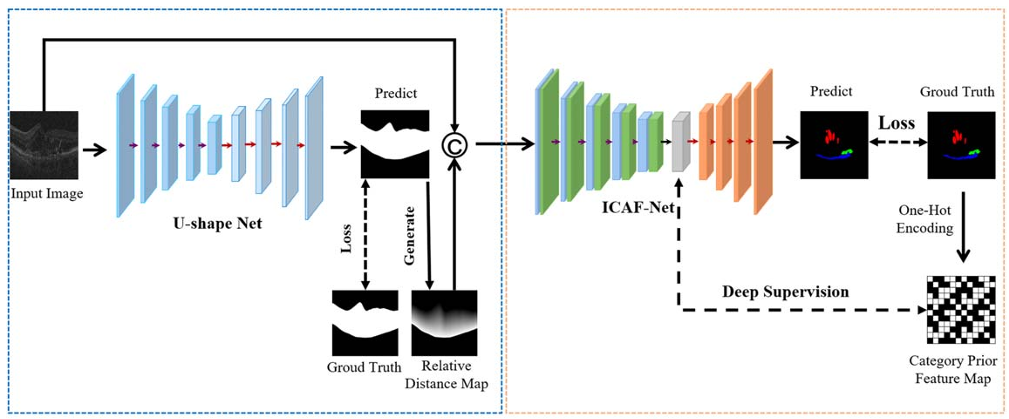
\includegraphics[width=1\linewidth]{figures/PreSegmentationAndFluidSegmentation.png}
	\caption{Example of a framework that includes retinal layer delimitation and construction of a relative distance map (left side). The generated map, together with the original image, serves as input to the segmentation network (denominated ICAF-Net, by the authors) \parencite{Tang2022}.}
	\label{fig:PreSegmentationAndFluidSegmentation}
\end{figure}
\par
Regarding the segmentation CNNs adopted by the analyzed papers, most are directly inspired by the U-Net, to which changes are done when considering the objectives of each study. Examples of such changes are the introduction of blocks (such as residual \parencite{Mantel2021, Zhang2023, Liu2024, Hassan2021b, Hassan2021a, Padilla2022}), and modules (like atrous sampling pyramid pooling \parencite{Hassan2021b, Hassan2021a, Hu2019, Sappa2021}), which makes the network distinctive. However, some papers use other variations of the U-Net that are also popular: the Deeplab \parencite{LChen2018} in \textcite{Hassan2021a, Li2023}, and the VGG \parencite{Simonyan2014} in \textcite{Padilla2022, Hassan2021b}.

\section{Intermediate Slice Synthesis}
For many years, there have been attempts to improve the resolution of OCT exams using computational methods, a process called super-resolution (SR). In 3D applications, such as magnetic resonance imaging (MRI), computed tomography (CT), and OCT, SR can be applied either intra-slice, improving the resolution of each slice in the volume along one plane, or inter-slice, enhancing the resolution of the volume along one axis by generating one or more slices between a pair of original ones. Some frameworks may even combine both approaches \parencite{You2020}.
\par
The use of GANs for generating slices between pre-existing slices is a commonly used technique in MRI and CT, but with few examples in OCT \parencite{You2020}. The systematic literature review performed by \textcite{Ibrahim2024}, which analyzed the latest trends in the use of generative models in medical data, only presents one example of GAN for inter-slice resolution improvement in OCT volumes \parencite{Lopez2023}. In this imaging technique, the use of GANs is mainly done for the generation of OCT images and conversion between different vendors \parencite{Ibrahim2024}.
\par
In the following subsection, the state-of-the-art architectures used for the improvement of inter-slice resolution are presented.

\subsection{Architectures for Medical Image Super-Resolution}
Given the lack of examples in OCT imaging, it was considered appropriate to study works from other imaging techniques, such as CT, MRI, and even video, given that the working principle is the same across them. The selected papers that are applied to medical images can be classified into three distinct categories: inter-slice SR, which leverages information from adjacent slices to generate one or more intermediate slices \parencite{Lopez2023, Xia2021, Wu2022, Nishimoto2024}; intra-slice SR combined with inter-slice SR, which improves the resolution of the slices from orthogonal planes and combines them with the results of inter-slice SR \parencite{Zhang2024, Peng2020, Fang2022, Nimitha2024, Georgescu2020}; and SR applied directly in 3D volumes, utilizing three-dimensional convolutions in the generation process, which incorporates the information along all the axes from multiple slices simultaneously \parencite{YChen2018, Sanchez2018, Kudo2019, Zhang2022}.
\par

\subsubsection{Inter-slice SR}

\textcite{Lopez2023} present an inter-slice SR framework based on a GAN, inspired by the ResNet, for the generation of three B-scan slices between two known slices. The GAN training process, as illustrated in Figure \ref{fig:GANGenerationFramework}, begins with the generation of an intermediate slice (Central Fake) located between two original B-scans (Pre and Post), which are separated by another original one (Central). The Central B-scan serves as the ground truth (GT) and is used in the assessment of the quality of the image generated by the network. Subsequently, the network generates other two slices: one between the Pre and Central slices, designated as Pre-Central fake, and another between the Central and Post slices, named Post-Central fake. Since these generated slices lack corresponding GT, the network's performance is regulated by using these two new synthetic slices for generating an additional intermediate slice (Central Fake 2), which is then compared to the true Central. Consequently, if the generation of Pre- and Post-Central fake images are inadequate, the Central Fake 2 will also be of poor quality, resulting in a higher loss value. During the inference process, one slice is synthesized for every two known B-scans, reducing the inter-slice distance to half of the original value.
\par
The importance of this study comes not only from it being the only study in OCT but also from the approach selected, which is similar to the foundation of the frameworks implemented in other papers. 

\begin{figure}[!ht]
	\centering
	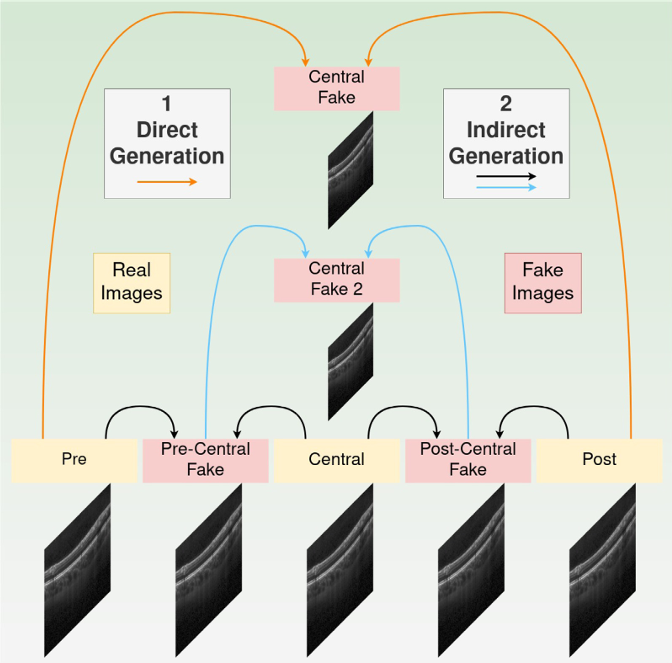
\includegraphics[width=0.70\linewidth]{figures/GANGenerationFramework.png}
	\caption{\textcite{Lopez2023} training process.}
	\label{fig:GANGenerationFramework}
\end{figure}

In a more straightforward approach, \textcite{Nishimoto2024} utilize a baseline U-Net that uses two spaced slices as input to generate the slices between them. This methodology was tested in the generation of three, four, and five intermediate slices, and obtained better outcomes than those generated through linear interpolation. This approach works particularly well due to the low noise present in the CT scans. In volumes with more noise, due to the presence of metal artifacts, the slices generated using the U-Net are of worse quality than those obtained through linear interpolation.
\par
The work by \textcite{Xia2021} demonstrates the enhancement of inter-slice resolution in MRI through the use of multiple networks and a multi-scale discriminator that considers both global and local features by processing different image scales and a scheme that illustrates this framework can be seen in Figure \ref{fig:XiaFramework}. The networks in this framework receive two slices ($x_{z\pm1}$) and generate a new one between them ($x_{z}$). The generator ($G$) is responsible for producing the intermediate slice, while the discriminator ($D$) learns to distinguish the synthesized image from the real image. The loss of these networks is also determined by the similarity of feature maps between images ($L_{FM}$).
\par
The framework contains two other U-shaped networks: one that learns to predict the optical flow and one that learns to predict the depth map for each input image. Based on the optical flow, depth maps, and their linear interpolation ($\bar{x_{z}}$), another U-shaped network generates the intermediate slice. The result from this network and the generator's output (to which Gaussian blurring is applied) are evaluated by the discriminator. Once again, the discriminator evaluates both images in separate feature spaces, processing each input at a different scale to extract both global and local representations for comparison.
\par
The image generated by the network using optical flow and depth ($\hat{x_{z}}$) pays special attention to the transitions between the two input slices. The point of inputting these images to the discriminator is to encourage it to recognize these characteristics in the generator's output. Additionally, the discriminator is exposed to blurred images to further incentive the generator to produce sharper images.

\begin{figure}[!ht]
	\hspace*{-0.35in}
	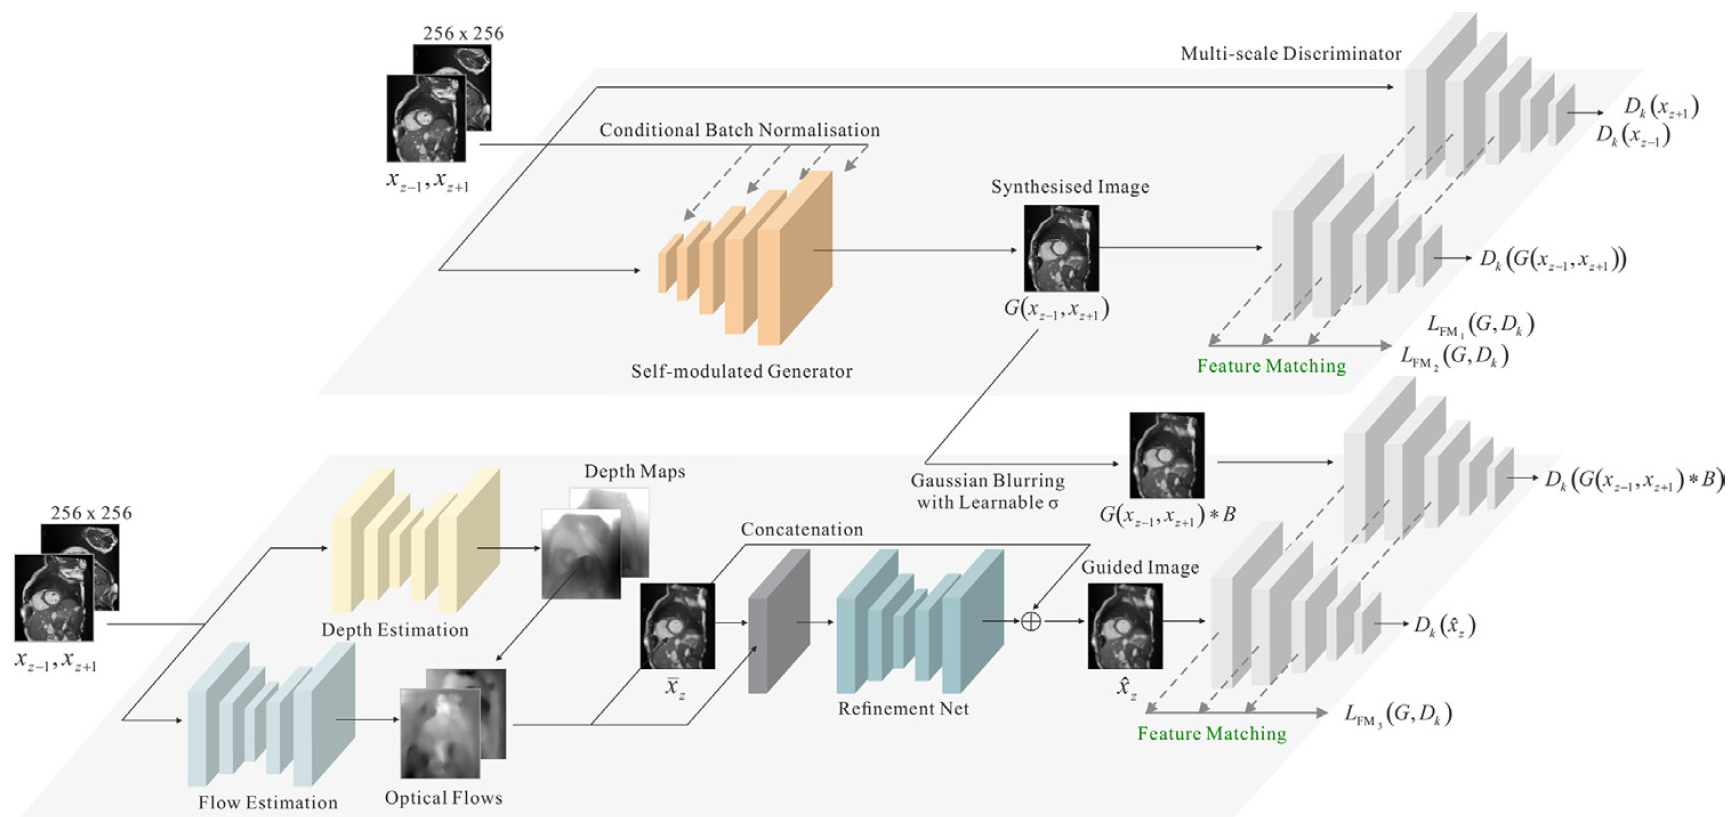
\includegraphics[width=1.1\linewidth]{figures/XiaFramework.png}
	\caption{Framework developed by \textcite{Xia2021}.}
	\label{fig:XiaFramework}
\end{figure}

\par
On the other hand, \textcite{Wu2022} improved the inter-slice resolution by training a generator network to output bi-directional spatial transformations instead of producing fake images. The advantage of this process is that it allows the same transformations to be applied to the segmentation masks from the surrounding slices, generating fake masks for the fake slices. 
\par
As in \textcite{Xia2021}, the GAN's discriminators also evaluate the generated images in both a larger and smaller field of view. To evaluate the output at a larger field of view, a global discriminator classifies the image as real or fake. Meanwhile, the evaluation at a smaller field of view integrates an attention network, which focuses on the most informative regions of the image to support the local discriminator and the object identifier. 
\par
The local discriminator classifies the image as real or fake based on fine-grained features extracted by the attention network. Meanwhile, the object classifier, which is a much shallower network, verifies whether certain structures present in the real image also appear in the fake one, using the output of the attention network. 
\par
By using both global and local discriminators, the generator is encouraged to output images that closely resemble the real images, both in the overall structure and fine details. The object detector ensures that the objects present in the real image are represented in the generated one.

\subsubsection{Intra- and Inter-slice SR}

As an example of combining intra-slice SR with inter-slice SR, \textcite{Zhang2024} implemented two networks that enhance the resolution of CT volume's slices in the two planes with the lowest in-slice resolution: sagittal and coronal. These networks increase the resolution only along the axial direction. The models here utilized are based on the anisotropic meta interpolation (AMI) network developed by \textcite{Peng2020}, a benchmark work in the field of medical image SR. 
\par
\textcite{Peng2020} introduced the AMI network as a single-image SR method designed to enhance the slice's resolution along the axis with the lowest spatial resolution - in this case, the axial axis. The AMI network is applied independently to the sagittal and coronal slices, generating complementary interpolations along the axial direction. A fusion network then combines these two outputs to synthesize high-resolution slices along the axial plane.
\par
The implementation by \textcite{Zhang2024} extends the use of the AMI network in the images of the sagittal and coronal planes by incorporating a GAN. This GAN takes two adjacent axial slices as input and generates an intermediate slice, with a framework that is similar to that of \textcite{Lopez2023}.
\par
The three networks are trained on downsampled CT scans from which every other axial slice is removed. The outputs of the sagittal and coronal AMI networks are compared to the corresponding slices in the original CT scans. Meanwhile, the GAN's output is compared to the GT axial slices from the original CT scan.
\par
Instead of using a dedicated fusion network as in \textcite{Peng2020}, \textcite{Zhang2024} introduce a loss function that directly compares the outputs of the AMI networks to the output of the GAN. This loss is backpropagated through the generator, encouraging it to output axial slices that are coherent with the content inferred by the AMI networks. This results in axial images that are not only visually consistent with the original CT slices but also integrate structural information from other anatomical planes. A scheme of this method is shown in Figure \ref{fig:ZhangFramework}.

\begin{figure}[!ht]
	\hspace*{-0.35in}
	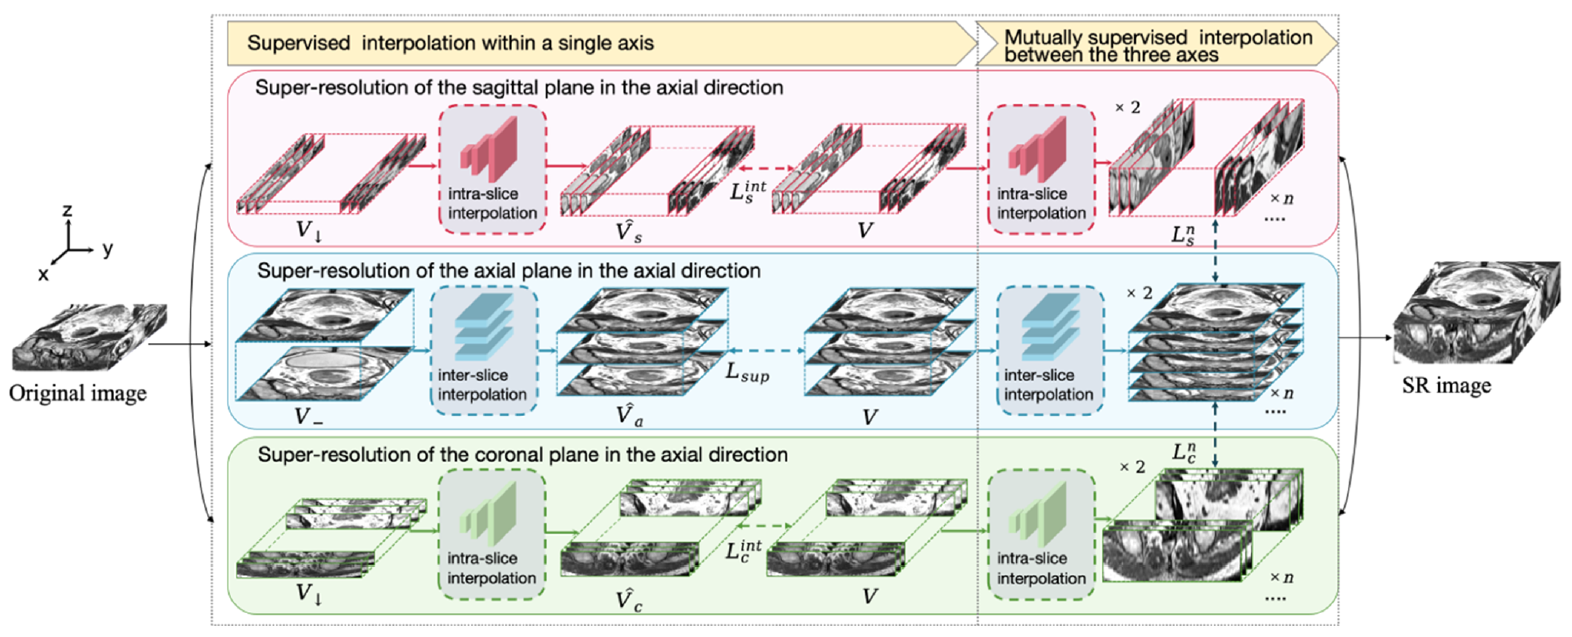
\includegraphics[width=1.1\linewidth]{figures/ZhangFramework.png}
	\caption{Architecture of the method developed by \textcite{Zhang2024}.}
	\label{fig:ZhangFramework}
\end{figure}

A similar approach was done by \textcite{Fang2022}. In this framework, three CNNs (one for each axis) are trained with the goal of generating the intermediate slices along the axis with a lower inter-slice resolution, which is the axial axis. Similarly to what is done in \textcite{Zhang2024}, two CNNs (one for the sagittal plane and one for the coronal plane) are trained to increase the resolution along the axial axis in the images of their respective plane. Both CNNs used in this work correspond to the single-image SR model developed by \textcite{Niu2020}. This CNN is an holistic attention network which improves the image's resolution by capturing both local and global contextual information. It uses holistic attention modules that combine channel attention (which emphasizes informative feature maps) and spatial attention (which highlights the most important regions of the image). This attention mechanism allows an image reconstruction with finer textures and sharper details in the super-resolved output.
\par
Instead of using a GAN to generate the intermediate slices along the axial plane, the authors apply another CNN. This network begins by extracting feature maps through space-to-depth transformation operations, which reorganize the spatial information into the channel dimension. The resulting features are then processed by a U-shaped architecture which captures both local and global context. Finally, a depth-to-space transformation is applied at the output layer, to reconstruct the intermediate axial slice at the original spatial resolution.
\par
All the networks are trained on downsampled CT volumes. After the first interpolation, all the outputs are compared to their respective GT and their loss is calculated. Then, another interpolation is performed in each axis, and a loss compares the generated images not with the GT, but with each other. This ensures coherence in the outputs predicted on different axis and transference of knowledge between them. During testing, inference is performed using a weighted prediction, with each axis' network contributing equally. In Figure \ref{fig:FangArchitecture}, the pipeline describing this implementation is shown.

\begin{figure}[!ht]
	\hspace*{-1.0in}
	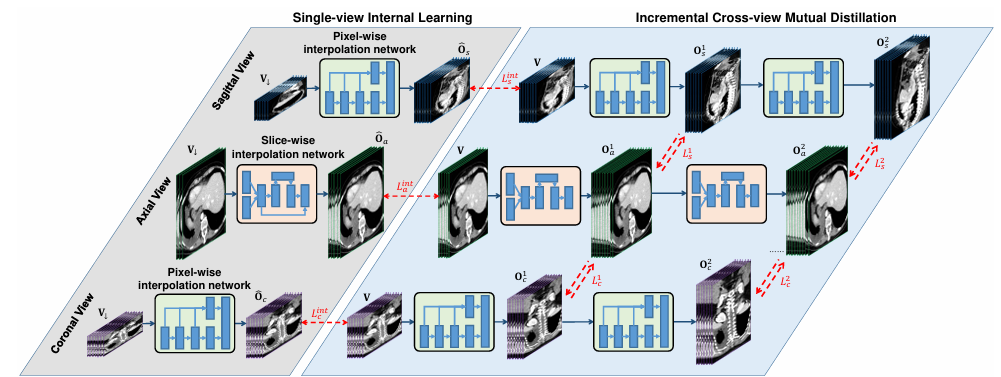
\includegraphics[width=1.25\linewidth]{figures/FangArchitecture.png}
	\caption{Pipeline of the methodology proposed by \textcite{Fang2022}.}
	\label{fig:FangArchitecture}
\end{figure}

\textcite{Nimitha2024} also perform intra-slice and inter-slice resolution enhancement. However, instead of improving both resolutions simultaneously as seen in \textcite{Zhang2024, Fang2022}, the enhancement is done sequentially. The pipeline starts with a low-resolution (LR) volume, in which axial slices are firstly enhanced to becoming high-resolution (HR). Based on these HR axial slices, an intermediate slice is generated between each pair of consecutive axial slices.
\par
The network used in the enhancement of intra-slice resolution is a GAN. The generator starts with an in-plane and out-of-plane attention modules that extract features from the MRI slices adjacent to the target one. These extracted features are then passed through a U-shaped network that reconstructs the intermediate image. However, the number of upsampling blocks is higher than the number of downsampling blocks to ensure that the output has higher spatial resolution than the input.
\par
To generate the intermediate slices, the compression-driven frame interpolation (CDFI) network, a state-of-the-art video frame interpolation CNN developed by \textcite{Ding2021}, was utilized. CDFI is built on top of the AdaCoF module \parencite{Lee2020}, which is particularly powerful at handling a wide range of motions between images.
\par 
The CDFI network first extracts features using a U-Net architecture. These features are passed from the U-Net encoder to a pyramid network with the same number of levels as the encoder. At each level, a 1x1 convolution is applied to the feature maps to reduce dimensionality and prepare them for motion estimation.
\par
Two sub-networks take the U-Net's output and estimate the parameters of the AdaCoF operation. The U-Net's output is also combined with an occlusion mask to create the first candidate intermediate slice.
\par
The pyramid network's outputs are warped using AdaCoF and then passed into a synthesis network, which generates the second candidate intermediate slice. The two candidate intermediate slices are combined through a second occlusion mask to generate the final output. This model maintains visual realism from the first slice while ensuring a coherent pixel movement by using the second slice.
\par
\textcite{Georgescu2020} used a similar approach for enhancing intra- and inter-slice resolution in CT and MRI scans through two separate CNNs. One CNN was tasked with enhancing the resolution of the LR slices. Concurrently, the other CNN was utilized to reduce the distance between slices by increasing the resolution of the images from the orthogonal plane. By inferring an image with increased resolution along this plane, new intermediate slices were generated, improving the inter-slice resolution along the low resolution axis.
\par
The CNNs for intra- and inter-slice resolution are similar. Both networks consist of 10 consecutive convolutional layers, with the first 5 having 32 filters. The number of filters in the following layers changes according to the output size. This output size differs between the two CNNs because the first increases the resolution in two directions, while the other only increases the resolution in one direction.

\subsubsection{Three-dimensional SR}

The methodologies that use 3D GANs are similar to one another, as they all employ network architectures based on those used in 2D images. As the 3D GANs already considers the information across all the axes simultaneously, there is no need to use multiple networks for each, as seen in some of the previous approaches. Therefore, the differences between papers mainly originate from the medical imaging technique to which it is applied, the modules that constitute the 3D GANs used, and the datasets used for evaluation \parencite{YChen2018, Sanchez2018, Kudo2019, Zhang2022}.

\subsubsection{Video Frame Interpolation for Inter-slice SR in Medical Imaging}

Applications to increase the number of frames per second in a video work based on the same principle as the implementations that increase the inter-slice resolution of the three-dimensional volumes in medical images. In order to increase the number of frames in a video, these frameworks utilize two consecutive frames to generate an intermediate one, which is similar to what is seen in the previous papers that perform intermediate slice generation in medical images. The key difference between these applications is that, in video, the physical quantity that separates the frames is time, while the physical quantity that separates slices in medical imaging volumes is distance \parencite{Fang2022, Gambini2024}.
\par
Believing that the concepts that work on video also work on CT and MRI, \textcite{Gambini2024} implemented a state-of-the-art method of video interpolation to generate intermediate slices in CT and MRI. The method used was the real-time interpolation flow estimation (RIFE) \parencite{Huang2022}. The CNN incorporated in RIFE learns the pixel movements between frames from numerous examples. This approach, called contextual flow, appears as an alternative to optical flow - a method commonly utilized to describe the movement between frames which attempts to predict pixel movements by calculating their movement between consecutive frames. RIFE is also aware of the time difference between frames, which translates to the distance between slices in CT and MRI. To construct the middle image, the network learns how to blend the previous and following image so that the generated intermediate one looks more similar to the expected, combining it with the contextual flow. Lastly, a second network is used in the refinement of the generated image.
\par
Both networks learn based on a loss function that has three components: a photometric loss that determines how close the generated image is to the GT; a perceptual loss which evaluates the generated image as the human perception would; and a smoothness loss that evaluates how smooth the generated image is \parencite{Huang2022}.

\begin{figure}[!ht]
	\centering
	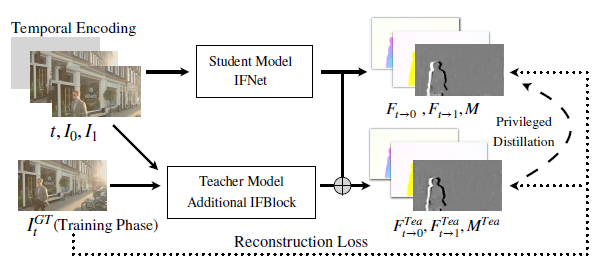
\includegraphics[width=0.85\linewidth]{figures/RIFEPipeline.png}
	\caption{Pipeline that describes the RIFE framework. The student model attempts to generate the intermediate frame, while the teacher refines the frame generated by the student so that it looks more similar to the middle frame. The results from both networks are evaluated on the reconstruction loss \parencite{Huang2022}.}
	\label{fig:RIFEPipeline}
\end{figure}

\textcite{Tran2020} present an alternative framework to the video frame interpolation. Instead of relying on contextual or optical flow to model pixel changes, two GANs are used for predicting the intermediate frame. The first generator receives as input the previous and following slice of the one desired to segment. The resulting slice is evaluated using the generator loss, which is composed of four components. This loss assesses how accurately the image is reconstructed and evaluates how well it fools the discriminator.
\par
The image resulting from the generator is given as input to the discriminator, which receives real and fake images as input and is responsible for correctly classifying it. The discriminator's prediction is compared to the true image's label, and the resulting loss is used in the adjustment of the generator weights.
\par
After training the first GAN, the second one is trained, which is a pix2pix \parencite{Isola2017}. Similar to what is seen in the work of \textcite{Gambini2024, Huang2022}, where a second network is used in the refinement of the output of the first one, this GAN is responsible for making the image output from the first GAN more similar to the original image. Contrasting with the previous examples where both the generative and refining networks are trained at the same time, the refining network is trained independently, after the training of the first network. The pipeline that describes this framework is shown in Figure \ref{fig:VideoGANFramework}.

\begin{figure}[!ht]
	\centering
	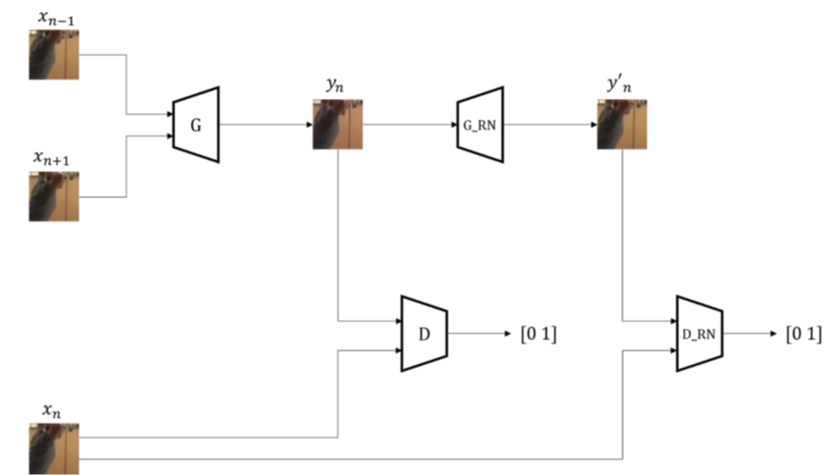
\includegraphics[width=1.0\linewidth]{figures/VideoGANFramework}
	\caption{Pipeline representing the framework developed by \textcite{Tran2020}. The generator that produces the intermediate frame is represented by $G$, while the discriminator is labeled $D$. The pix2pix generator is denoted by $G\_RN$ and the discriminator is represented by $D\_RN$. $x_{n-1}$ and $x_{n+1}$ respectively represent the previous and following frames of the one that is being generated, $x_{n}$. $y_{n}$ is the image generated by the first generator, while $y'_{n}$ is the image refined by the pix2pix network \parencite{Tran2020}.}
	\label{fig:VideoGANFramework}
\end{figure}

\chapter{Methods}\label{Methods}
The Methods section starts with an overview of the dataset selected for the fluid segmentation and intermediate slice synthesis tasks, while regarding the requirements needed for the training of each model and the reasoning behind the selection. Afterwards, it provides an explanation of the experiments that were performed during the dissertation, regarding fluid segmentation, inter-slice generation, and fluid volume estimation, while explaining the methodologies that were implemented.

\section{Dataset}
The application of deep learning to fluid segmentation in OCT volumes requires a large number of images annotated with the three retinal fluids for the training process. The manual segmentation of large amounts of B-scans is a laborious process, which results in a shortage of publicly available annotated OCT datasets. Consequently, the majority of these datasets contain a limited quantity of images.
\par
The dataset selected for this dissertation is the RETOUCH dataset \parencite{Bogunovic2019b}. This dataset consists of 112 OCT volumes, obtained with four different devices: 38 from the Cirrus HD-OCT (Zeiss Meditec), 38 from the Spectralis (Heidelberg Engineering), and 36 from the \mbox{T-1000}/T-2000 (Topcon). The 112 volumes are split into training (70 volumes) and testing (42 volumes). Only those in the training set have annotations of the retinal fluids (IRF, SRF, and PED). For the training and testing of the segmentation models, only the annotated volumes were used.
\par
From the 70 volumes, 24 were obtained with the Cirrus, 24 volumes were acquired with the Spectralis, and 22 were obtained with the two Topcon devices. The number of B-scans per volume, the dimensions of the B-scans, and the axial resolutions vary according to the device utilized to obtain the OCT. The volumes acquired using the Cirrus have 128 B-scans, while those obtained with Spectralis have 49 B-scans. The volumes acquired using Topcon devices (\mbox{T-1000} or \mbox{T-2000}) have 128 B-scans, but there are two volumes that only contain 64 \mbox{B-scans}. In total, 6838 B-scans were used on the train and test of the segmentation models.
\par
When compared with other renown OCT datasets annotated with retinal fluid, such as the Duke dataset \parencite{Chiu2015}, the two datasets from the University of Minnesota \parencite{Rashno2017, Rashno2018}, and the \textcite{Lu2019} dataset, the RETOUCH presents a significantly larger quantity of annotated volumes. It also shows more variety since the volumes were obtained using four different devices instead of including volumes from just one device, as done in the mentioned datasets. In Table \ref{tab:DatasetsSummary}, a comparison between the number of annotated B-scans in each of the mentioned datasets is shown, as well as the devices utilized to obtain the OCT images, the diseases of the patients, and the distribution of annotated B-scans per OCT volume.

\begin{table*}[!ht]
	\caption{Volumes, B-scans per volume, the total number of B-scans, and macular diseases in each dataset.}
	\centering
	\resizebox{\textwidth}{!}{\begin{tabular}{|c|c|c|c|c|c|}
		\hline
		& & & & & \\ [-1.5ex] % Used to center the text vertically
		& \textbf{DUKE2015 \cite{Chiu2015}} & \textbf{UMN2017 \cite{Rashno2017}} & \textbf{UMN2018 \cite{Rashno2018}} & \textbf{LU2019 \cite{Lu2019}} & \textbf{RETOUCH \cite{Bogunovic2019b}} \\ [1ex]
		\hline
		& & & & & \\ [-2.0ex]
		\textbf{Volumes} & 10 & 24 & 29 & 528 & 70$^{a}$ \\
		& & & & & \\ [-2.5ex]
		\textbf{B-scans/Volume} & 11 & 25 & 25 & Variable & 128 (Cirrus and Topcon$^{b}$), 64 (Topcon$^{b}$), 49 (Spectralis) \\
		& & & & & \\ [-2.5ex]
		\textbf{B-scans} & 110 & 600 & 725 & 750 & 6838 \\
		& & & & & \\ [-2.5ex]
		\textbf{Device} & Spectralis & Spectralis & Spectralis & Spectralis & Cirrus, Topcon and Spectralis \\
		& & & & & \\ [-2.5ex]
		\textbf{Disease} & DME & AMD & DME & DME & AMD and RVO \\
		\hline
		\multicolumn{4}{l}{}
	\end{tabular}}
	\label{tab:DatasetsSummary}
	\par
	\justifying
	\footnotesize{$^{a}$ 24 volumes from Cirrus, 22 volumes from Topcon, and 24 volumes from Spectralis.}
	\par 
	\justifying
	\footnotesize{$^{b}$ Two of the training volumes obtained using the Topcon devices have only 64 slices.}
\end{table*}

\par
For these reasons, the RETOUCH dataset is regarded as a diverse and large dataset, widely used in the literature that aims to perform fluid segmentation using deep learning, as done in \parencite{Rahil2023, Zhang2023, Xing2022, Tang2022, Liu2024, Li2023, Hassan2021b, Lu2019}. These aspects motivated the selection of the RETOUCH as the dataset that was used for implementing the models for fluid segmentation in OCT volumes in this dissertation.
\par
In intermediate slice synthesis, the 112 OCT volumes that constitute the RETOUCH dataset were used for the training and evaluation of the models. The volumes that do not have segmentation masks can also be included since these masks are not necessary in the intermediate slice generation task.
\par
The consistent number of slices per volume and large quantity of OCT volumes make the RETOUCH dataset suitable for the training and evaluation of the models developed to generate intermediate slices.

\section{Experiments}\label{Experiments}
In this subsection, the experiments conducted during the dissertation are explained in depth. The subsection begins with a description of how the data was split, followed by the experiments in fluid segmentation, intermediate slice generation, and in fluid volume estimation.
\par
All the experiments were conducted using an NVIDIA GeForce RTX 3080 GPU and the \hbox{PyTorch} machine learning library (version 2.5.1).

\subsection{Cross-validation}\label{CrossValidation}
To promote consistency across all experiments, the conditions were held identical. In every experiment, the train-test split followed a 5-fold split, with different splits being used for the segmentation and generation tasks. During training, all the images in three folds were utilized to train the model, while the images from one fold were used in its validation. One fold was reserved and used to compare the performance between the best model from different experiments. Therefore, four training runs are completed in each experiment, rotating the validation fold across runs. The reserved fold consists of the same OCT volumes for all experiments, allowing for further comparisons on data not seen by any of the models.
\par
The images in the fold that was used in validation allowed an insight of how the model was learning. In the segmentation experiments, the instance of the model that achieved the lowest loss on validation data was saved, as this typically indicates the best generalization performance on unseen data. Also, when the model was no longer improving, training could be stopped, saving computational resources.
\par
The dataset was split so that the quantity of each fluid per vendor and the number of volumes per vendor was equally distributed across the folds. By equally distributing the volumes, it is easier to assess the model's learning capability and its behavior towards data with different characteristics (e.g. data from different vendors). To accomplish a fair data split, a custom algorithm was elaborated. This algorithm sought to divide the data in five folds while minimizing the differences of fluid per vendor and the number of slices per vendor in each fold.
\par
A possible distribution of 70 OCT volumes from the RETOUCH dataset, which were used in the training of fluid segmentation, can be seen in Table \ref{tab:FiveFoldSplit}. The split was applied to the volumes and not to the slices. The slices of the same volumes must be kept together to prevent data leakage, where similar images, obtained from the same patient, are present both in training and validation, leading to over-optimistic performance metrics.

\begin{table*}[!ht]
	\setlength{\tabcolsep}{6pt}
	\renewcommand{\arraystretch}{1.3}
	\caption{Number of OCT volumes per vendor in each fold, considering 5-fold validation.}
	\centering
	\begin{tabular}{|c|c|c|c|c|c|}
		\hline
		\textbf{Vendors} & \textbf{1$^{st}$} & \textbf{2$^{nd}$} & \textbf{3$^{rd}$} & \textbf{4$^{th}$} & \textbf{5$^{th}$} \\
		\hline
		\textbf{Cirrus} & 5 & 5 & 5 & 5 & 4 \\
		\textbf{Spectralis} & 5 & 5 & 5 & 5 & 4 \\
		\textbf{Topcon} & 4$^{a}$ + 1$^{b}$ & 4$^{a}$ + 1$^{b}$ & 4$^{a}$ & 4$^{a}$ & 4$^{a}$ \\
		\hline
		\multicolumn{4}{l}{Volumes marked with \textbf{\textit{a}} consist of 128 B-scans.} \\
		\multicolumn{4}{l}{Volumes marked with \textbf{\textit{b}} consist of 64 B-scans.}
	\end{tabular}
	\label{tab:FiveFoldSplit}
\end{table*}

In \ref{Experiment2} Experiment 2, where the model performs binary segmentation of each fluid, the volumes can be redistributed using the same algorithm, with less bounds. In this experiment, it is relevant to split the volumes in folds based only on their vendors and quantity of the fluid to segment, thus eliminating the restrictions imposed by the quantity of other two fluids. Nevertheless, the volumes that are in the previously defined reserved fold can not be used nor in training nor in validation.
\par
In the interslice generation experiments, the 5-fold split was not done by considering the fluids quantity in each fold. Since in this experiment the test volumes of the RETOUCH dataset were used and there are no fluid masks available, the quantity of fluid in each test volume is unknown. However, one of the folds in the interslice 5-fold split is the one reserved in the multi-class segmentation split.
\par
The split was performed by taking into consideration solely the number of slices per device. In this experiments, the characteristic's of each device are important, since each device has a specific interslice distance, which is different even across devices of the same vendor and an important characteristic in image generation.
\par
Considering both training and testing volumes of the RETOUCH dataset, there are 38 Cirrus, 38 Spectralis, 13 Topcon T-1000 and 23 Topcon T-2000 (two of which with 64 slices). The fold reserved in the multi-class segmentation task is composed of the following volumes: 4 Cirrus, 5 Spectralis, 3 Topcon T-1000, and 2 Topcon T-2000 (one of which with 64 slices). The volumes remaining for the four folds used in the generation task can be distributed as in the Table \ref{tab:FourFoldSplit}.

\begin{table*}[!ht]
	\setlength{\tabcolsep}{6pt}
	\renewcommand{\arraystretch}{1.3}
	\caption{Number of OCT volumes per device in each fold, in the four remaining folds.}
	\centering
	\begin{tabular}{|c|c|c|c|c|}
		\hline
		\textbf{Devices} & \textbf{1$^{st}$} & \textbf{2$^{nd}$} & \textbf{3$^{rd}$} & \textbf{4$^{th}$} \\
		\hline
		\textbf{Cirrus} & 9 & 9 & 8 & 8 \\
		\textbf{Spectralis} & 9 & 8 & 8 & 8 \\
		\textbf{T-1000} & 5 & 5 & 5 & 4 \\
		\textbf{T-2000} & 3 & 2 & 2 & 2 \\
		\textbf{T-2000$^{a}$} & 1 & 0 & 0 & 0 \\
		\hline
		\multicolumn{5}{l}{\textbf{\textit{a}}: volumes with 64 B-scans.} \\
	\end{tabular}
	\label{tab:FourFoldSplit}
\end{table*}

Since the partition is not bounded by the quantity of fluid in each volume, it is possible to compute the best partition by iterating through all the possible combinations. In each combination, the standard deviation of the total number of B-scans in each fold is calculated. The combination with the smallest deviation was used. 
\par
Similar to what was done in the fluid segmentation task, three folds was used in training while one was used in validation. The reserved fold was used as a comparison between the best generative models from different experiments.

\subsection{Fluid Segmentation}
The initial experiments of this dissertation focused on training networks on the fluid segmentation task. The goal of these experiments is to determine which segmentation network performs the best in the considered task, which were later required for the fluid volume estimation.
\par
In these experiments, the U-Net \parencite{Ronneberger2015} was used in the multi-class segmentation of the fluid regions in each B-scan. The U-Net is distinguished by its encoder-decoder structure, which resembles the letter U (see Figure \ref{fig:UNet}). In the encoder path, two 3x3 unpadded convolutions are applied to the input image, with each being followed by a rectified linear unit (ReLU) and a 2x2 max pooling operation with a stride of 2, downsampling the image. In each downsampling step, the number of channels is doubled. In the expanding path, a 2x2 up-convolution is used, resulting in the halving of the number of channels. The result is then concatenated with the cropped feature map from the respective contracting path. A 1x1 convolution is applied to the final layer.

\begin{figure}[!ht]
	\centering
	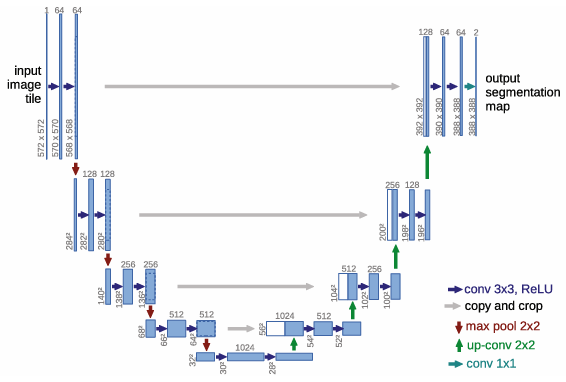
\includegraphics[width=0.75\linewidth]{../figures/UNet}
	\caption{U-Net architecture \cite{Ronneberger2015}.}
	\label{fig:UNet}
\end{figure}

The evaluation of all networks was conducted using the Dice coefficient. The Dice coefficient is a commonly used metric for evaluating the similarity between two sets. In this context, it was used for assessing the similarity between the segmentation mask generated by the segmentation network and the GT. The equation that describes the Dice coefficient can be seen in Equation \ref{eq:DiceCoefficient}, where $A$ is a set that represents the GT binary mask of one fluid and $B$ is another set that represents the predicted binary mask of the same fluid \cite{Shamir2019}. Considering $a_{i}$ and $b_{i}$ the binary pixels, the Dice coefficient can be rewritten as shown in Equation \ref{eq:DiceCoefficientPixels}. The network that performed the best was selected to estimate the fluid volumes in the fluid volume estimation experiments.

\begin{equation}
	\text{Dice}(A, B) = \frac{2|A \cap B|}{|A| + |B|}
	\label{eq:DiceCoefficient}
\end{equation}

\begin{equation}
	\text{Dice}(A, B) = \frac{2\sum_{i} a_{i} b_{i}}{\sum_{i} a_{i} + \sum_{i} b_{i}}
	\label{eq:DiceCoefficientPixels}
\end{equation}

The loss function that regularized the training in the fluid segmentation experiments was the same as the one used in \textcite{Tennakoon2018}, whose segmentation model was previously implemented by the authors. This loss is described as seen in Equation \ref{eq:SegmentationLoss}, where $\lambda_{D}$ is the weight of the Dice component, $\mathcal{L}_{D}$, and $\lambda_{CE}$ is the weight of the cross-entropy component, $\mathcal{L}_{CE}$, with both weights being 0.5.

\begin{equation}
	\mathcal{L} = \lambda_{D} \mathcal{L}_{D} + \lambda_{CE} \mathcal{L}_{CE}
	\label{eq:SegmentationLoss}
\end{equation}

The component $\mathcal{L}_{D}$ is the Dice loss of the foreground. This translates to how good the model is at detecting and segmenting the fluid present in the B-scans. For any image, where each pixel is associated with an index $i$, the loss can be described through Equation \ref{eq:SegmentationDice}, where $s_{i\overline{0}}$ is a binary variable that is 0 when the pixel $i$ belongs to the class 0 (background) and is 1 whenever the pixel $i$ belongs to any class that is not 0 (foreground). $p_{i\overline{0}}$ corresponds to the predicted probability of the pixel $i$ belonging to the foreground. The $\epsilon$ constant is a small value utilized to prevent division by zero.

\begin{equation}
	\mathcal{L}_{D} = 1 - \left( \frac{2 \sum_{i} s_{i\overline{0}} p_{i\overline{0}}}{\sum_{i} s_{i\overline{0}} + \sum_{i} p_{i\overline{0}} + \epsilon} \right)
	\label{eq:SegmentationDice}
\end{equation}

However, this loss component is not enough to correctly label the pixels in their respective classes and, for that reason, the cross-entropy component was used. Due to the large class imbalance in the images, with the background occupying the majority of them, the cross-entropy is balanced by taking into account the number of pixels belonging to each class. The cross-entropy is calculated for each pixel of index $i$ belonging to the image. Then, for each class, the cross-entropy of all pixels in the image is summed, before being divided by the number of pixels that belong to the class. The mean of the values obtained for each class result finally in $\mathcal{L}_{CE}$, as can be seen in Equation \ref{eq:SegmentationCE}. In this equation, $N=4$ and is the number of classes, while $C$ is the set of possible classes, $\{0,1,2,3\}$, which corresponds, respectively, to background, IRF, SRF, and PED.

\begin{equation}
	\mathcal{L}_{CE} = - \sum_{c \in C} \frac{1}{N}\left( \frac{1}{\sum_{i} s_{i,c}} \sum_{i} s_{i,c} \text{ln} p_{i,c} \right)
	\label{eq:SegmentationCE}
\end{equation}

\subsubsection{Experiment 1}\label{Experiment1}
In the first experiment, the base U-Net model was trained to perform 2D multi-class segmentation of the retinal fluids in OCT volumes.
\par
This was the most extensive set of experiments, where many variables were tested. Different patch shapes, transformations, and hyperparameters were experimented, until the best training settings were determined. The best settings were then used in \ref{Experiment2} Experiment 2. All the experiments were done using the Adam optimizer \parencite{Kingma2017} with a learning rate of $2 \times 10^{-5}$.

\paragraph{Experiment 1.1}
The model was initially trained on patches of size 256 $\times$ 128 (H $\times$ W), following the same implementation as the one in \textcite{Tennakoon2018}. The extraction of patches aims at prioritizing the B-scan information relevant for the segmentation. To achieve this, the patches are not distributed uniformly. Instead, 10 patches are extracted from a random location inside the region of interest (ROI) of each image. The image's ROI is the part of the image where the entropy is above a determined threshold or where retinal fluid is present. The patches are then randomly transformed by a rotation between 0 and 10 degrees, and horizontal flipping. Of the patches with no fluid, 75\% of them were dropped. In Figure \ref{fig:FluidAndROI}, it is possible to see the overlaying of the fluid masks and the ROI, with a red bounding box signaling a patch that would be used as input to train the U-Net.

\begin{figure}[!ht]
	\centering
	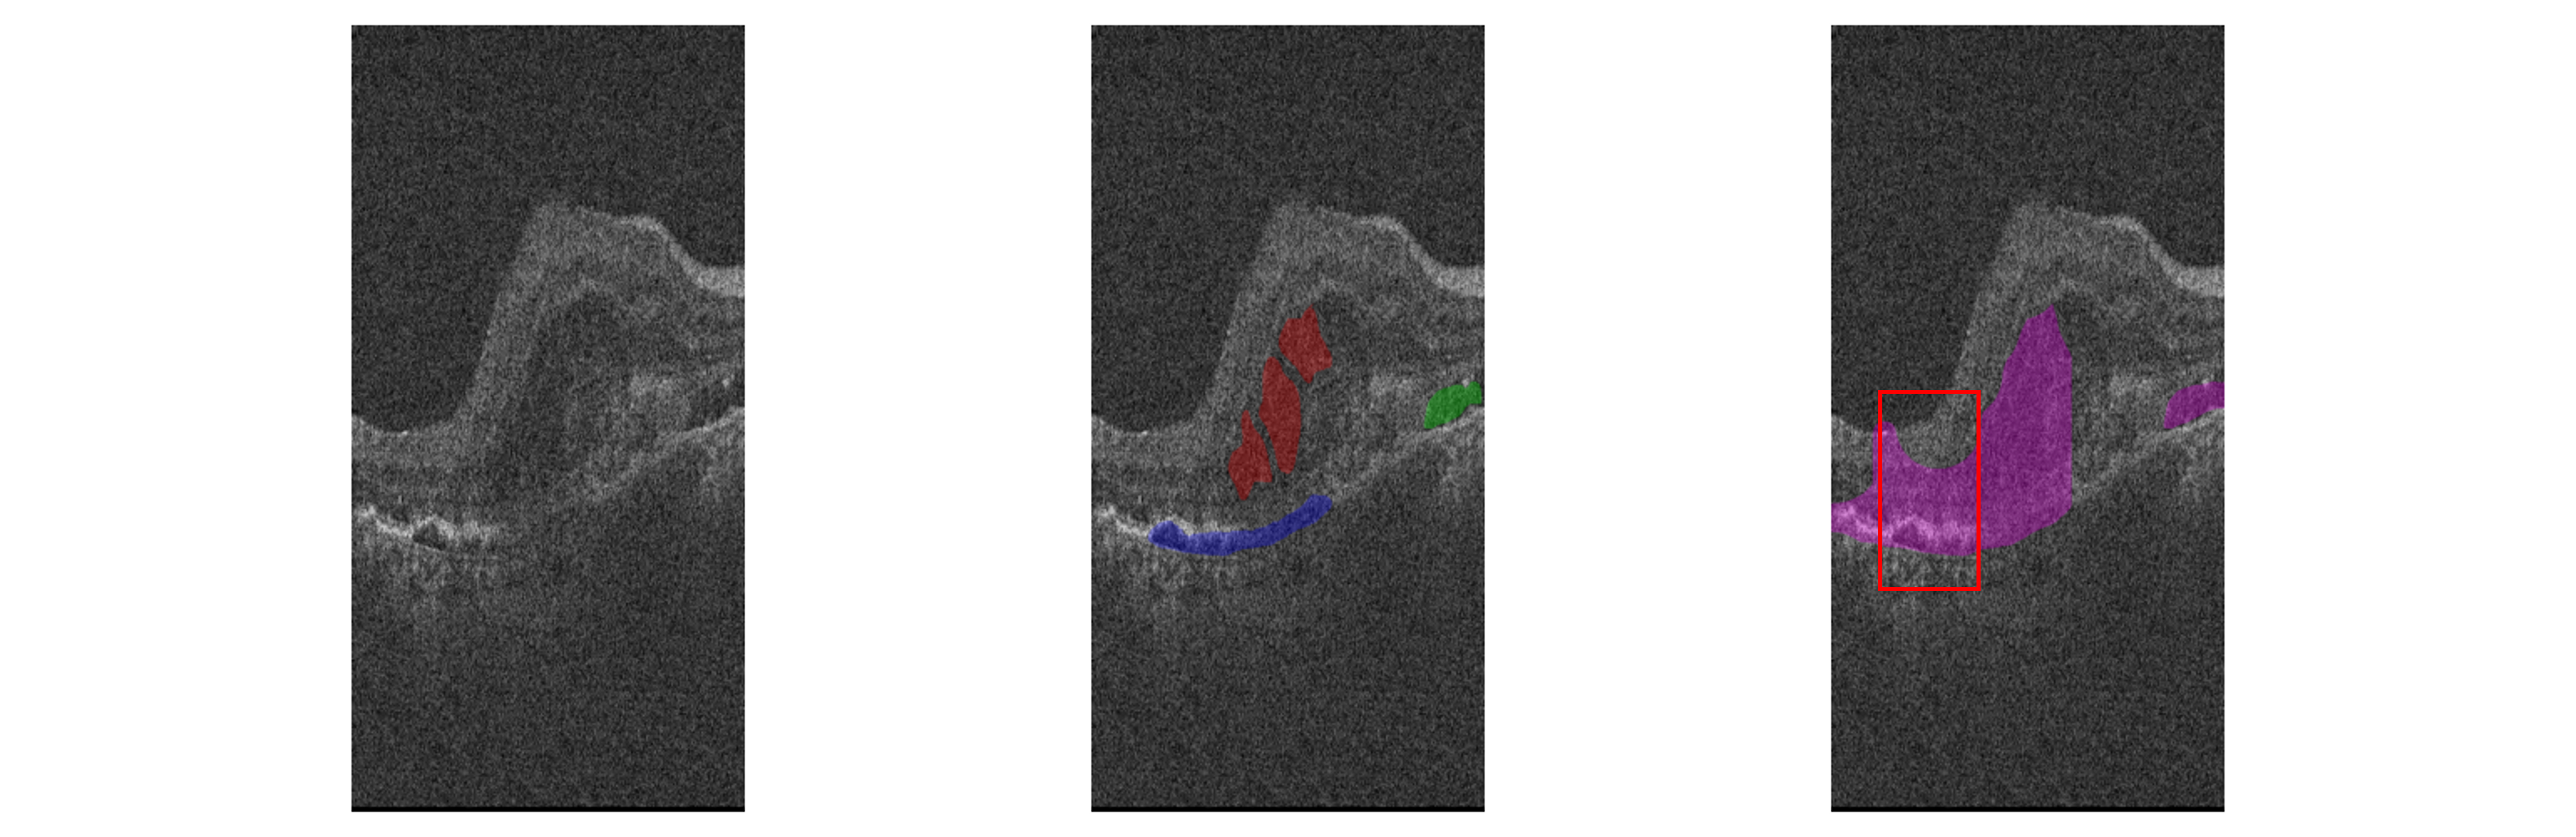
\includegraphics[width=1.0\linewidth]{../figures/FluidAndROI.png}
	\caption{Cirrus B-scan (left), fluid masks overlay (middle) with IRF in red, SRF in green, and PED in blue, and the ROI mask overlaid in purple (right). The red bounding box signals a possible 256 $\times$ 128 patch that could be extracted.}
	\label{fig:FluidAndROI}
\end{figure}

\par
In the Experiment 1.1, two sets of four training runs were performed, using each fold as validation. In both sets, the conditions were exactly the same, except the input patches, aiming to understand the effect that the random patch extraction has on the model's performances. The model was trained during 100 epochs with a batch size of 32, with no early stopping.

\paragraph{Experiment 1.2}
In Experiment 1.2, the patch shape was changed from 256 $\times$ 128 to 496 $\times$ 512. By using such shape, the model receives a larger context of the B-scan as input, allowing it to learn the anatomic references that characterize and limit the fluids.
\par
The patches used in this experiment were no longer randomly extracted from the ROI. Instead, the patches were extracted from top to bottom so that every section of the image would be present in at least one patch. In a Cirrus B-scan, with shape 1024 $\times$ 512, the first patch would correspond to section from $y=528$ to $y=1024$, while the second patch would be from $y=32$ to $y=528$. The last patch would then start on the bottom of the image, at $y=0$, to $y=496$. A representation of this process can be seen in Figure \ref{fig:BigPatchExtraction}. The patches are extracted from top to bottom so that the retina and the fluid would not be split in two patches, damaging the quality of the input data.
\par
In this experiment, due to the larger size of the patches that are being loaded, the batch size had to be reduced from 32 to 16. It was trained on 100 epochs with the same transformations as in the previous experiment and without early stopping.

\begin{figure}[!ht]
	\centering
	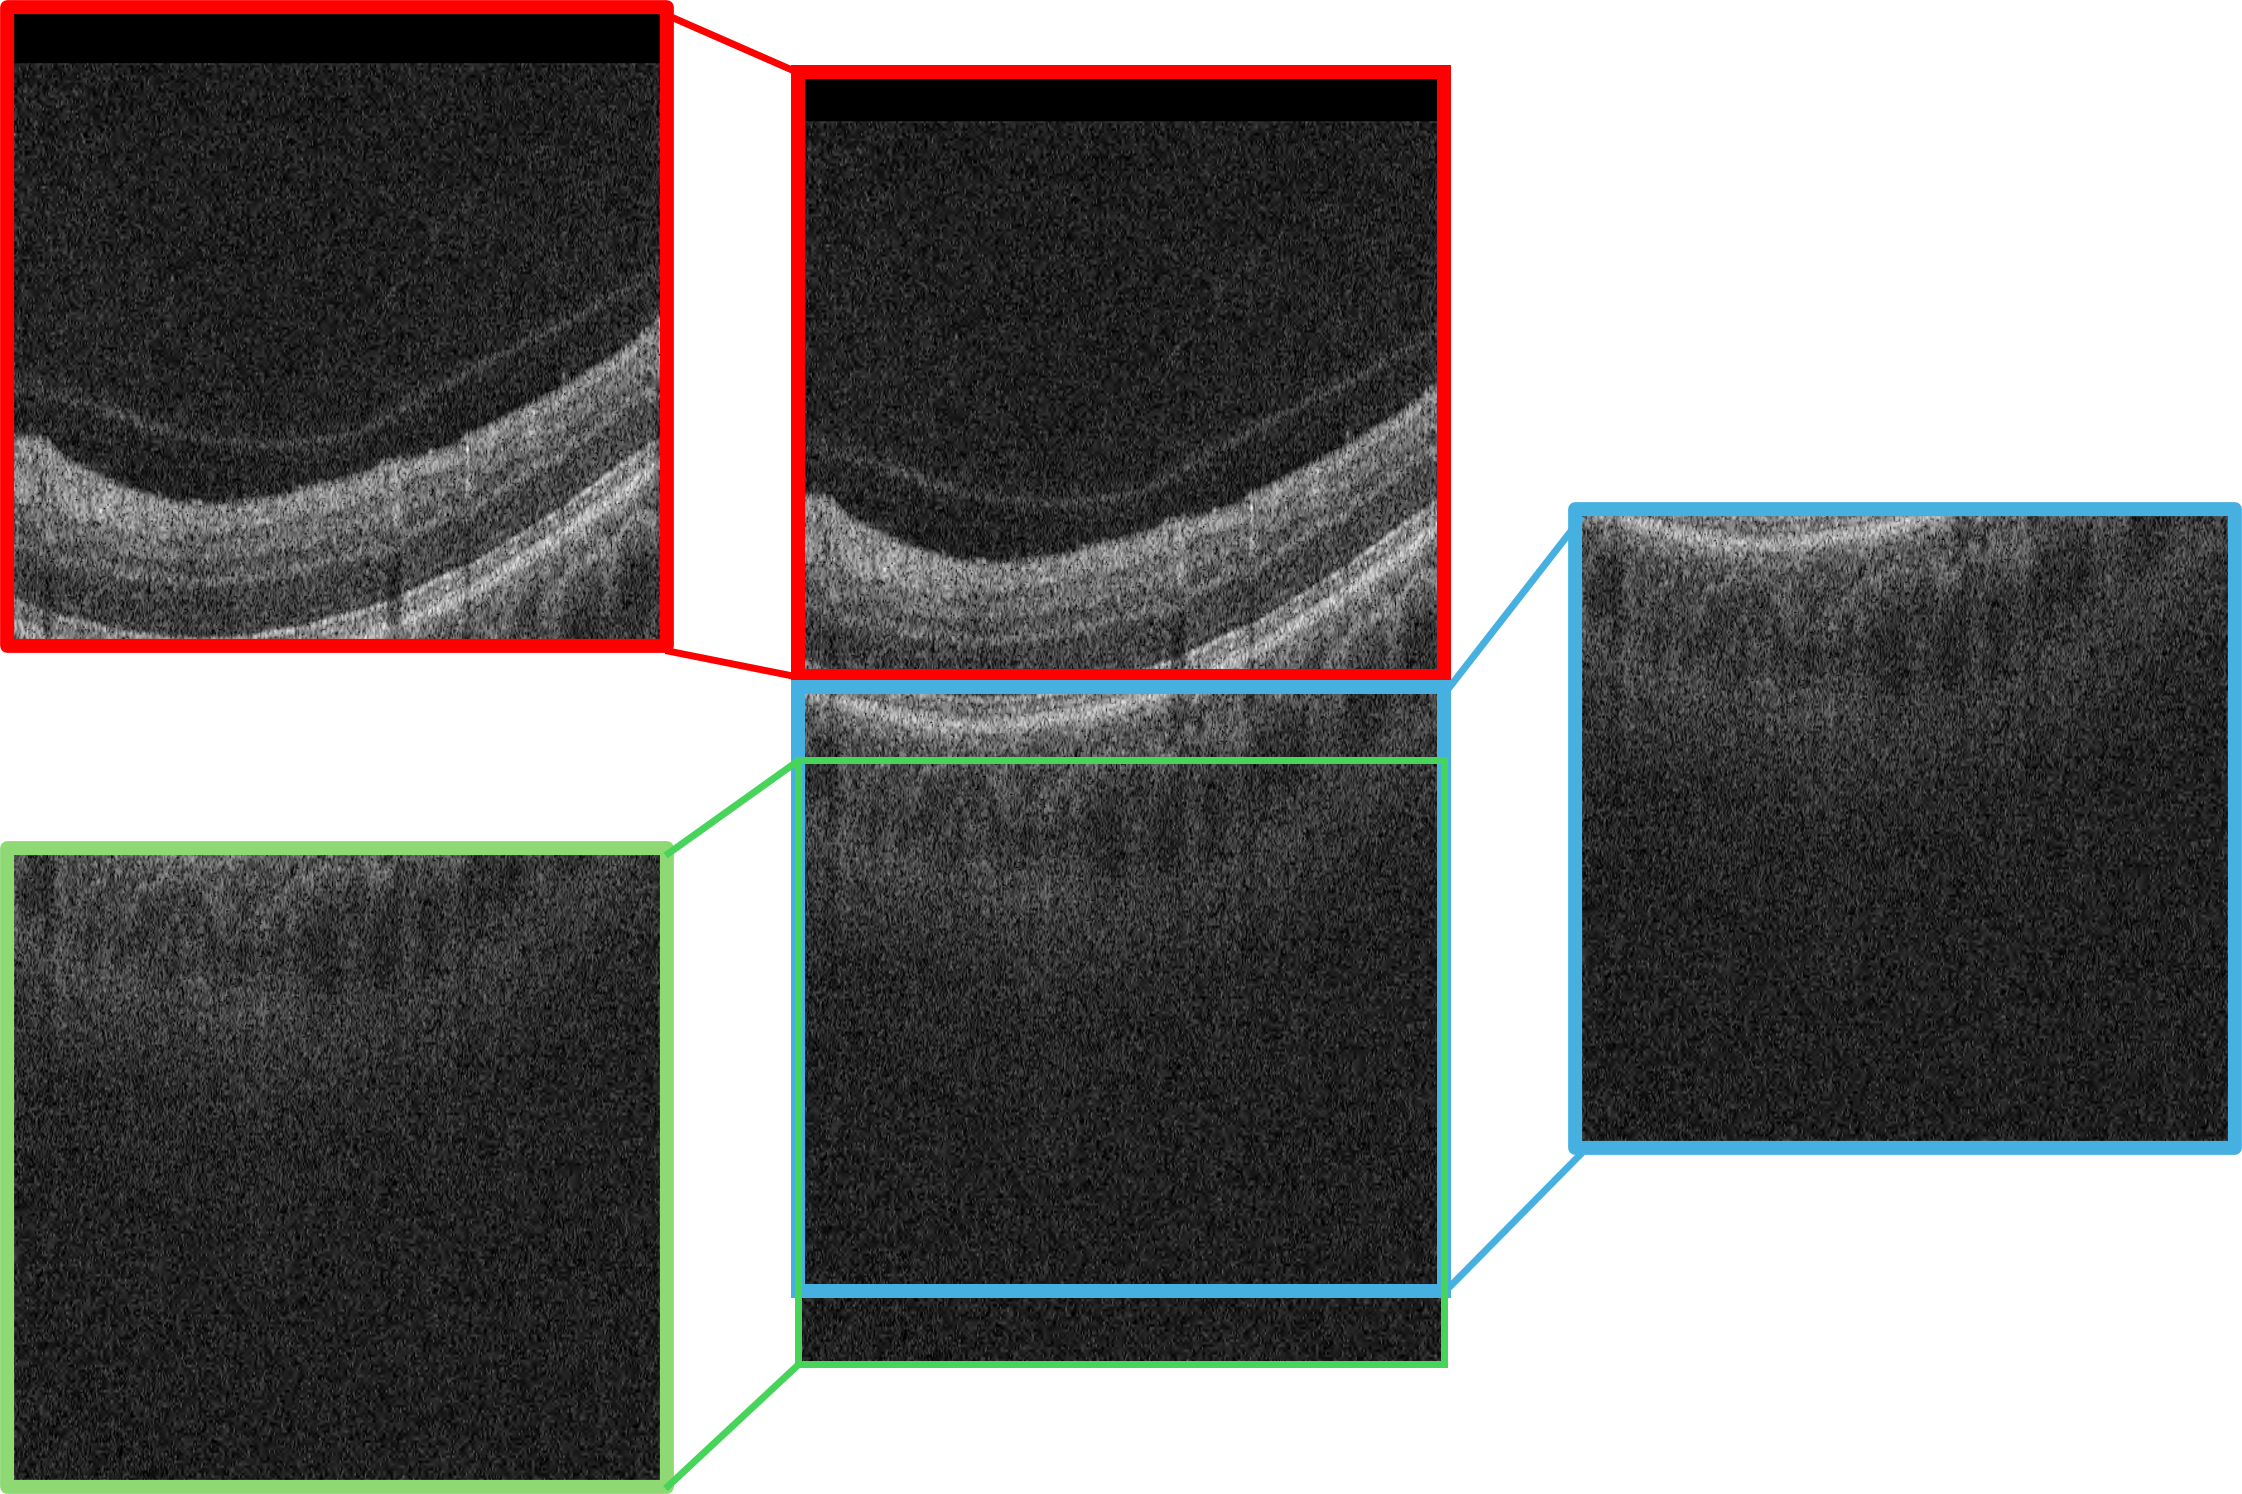
\includegraphics[width=0.4\linewidth]{../figures/BigPatchExtraction.png}
	\caption{Cirrus B-scan and its respective three patches of shape 496 $\times$ 512.}
	\label{fig:BigPatchExtraction}
\end{figure}

\paragraph{Experiment 1.3}
Another patch shape was experimented in Experiment 1.3. In this experiment, the images from different vendors were resized from their original dimensions to 496 $\times$ 512, the shape of the smaller images of the dataset, obtained with the Spectralis device. 
\par
The dimensions of the voxels in the OCT volumes change according to the device that was utilized to obtain the volume, resulting in images with different appearances across the vendors. For example, each voxel in the Cirrus volumes has an height of 1.95 $\mu$m, while each voxel in the Spectralis volumes has an height of 3.87 $\mu$m. For the same image, these differences in height lead to the same structures appearing bigger in Cirrus B-scans (see Figure \ref{fig:CirrusSpectralisRetinalLayerComparison}). These differences across vendors makes the learning of the segmentation harder. Therefore, by resizing all the images to the same shape, the structures would have more consistent dimensions across vendors and the voxels roughly translated to the same dimensions, leading to a easier learning process for the model.

\begin{figure}[!ht]
	\centering
	\includegraphics[width=0.4\linewidth]{../figures/CirrusSpectralisRetinalLayerComparison.png}
	\caption{B-scan of the retinal layers in different patients, using Cirrus (left) and Spectralis (right) devices. In Cirrus, the retinal layers appear much larger than in Spectralis.}
	\label{fig:CirrusSpectralisRetinalLayerComparison}
\end{figure}

Then, vertical patches, of shape 496 $\times$ 128, were extracted from each B-scan. The number of patches extracted from each image was changed, experimenting with four (Figure \ref{fig:CirrusFourPatchExtraction}), seven (Figure \ref{fig:CirrusSevenPatchExtraction}) and thirteen (Figure \ref{fig:CirrusThirteenPatchExtraction}) patches. The advantage of extracting vertical patches is that each image contains both the complete retinal layer and the background. This does not happen in the previous experiments, where the patches are either too small to contain both background and the retinal layers (in Experiment 1.1) or the retinal layers are cropped during patch extraction (in Experiment 1.2, as seen in Figure \ref{fig:BigPatchExtraction}).

\begin{figure}[!ht]
	\centering
	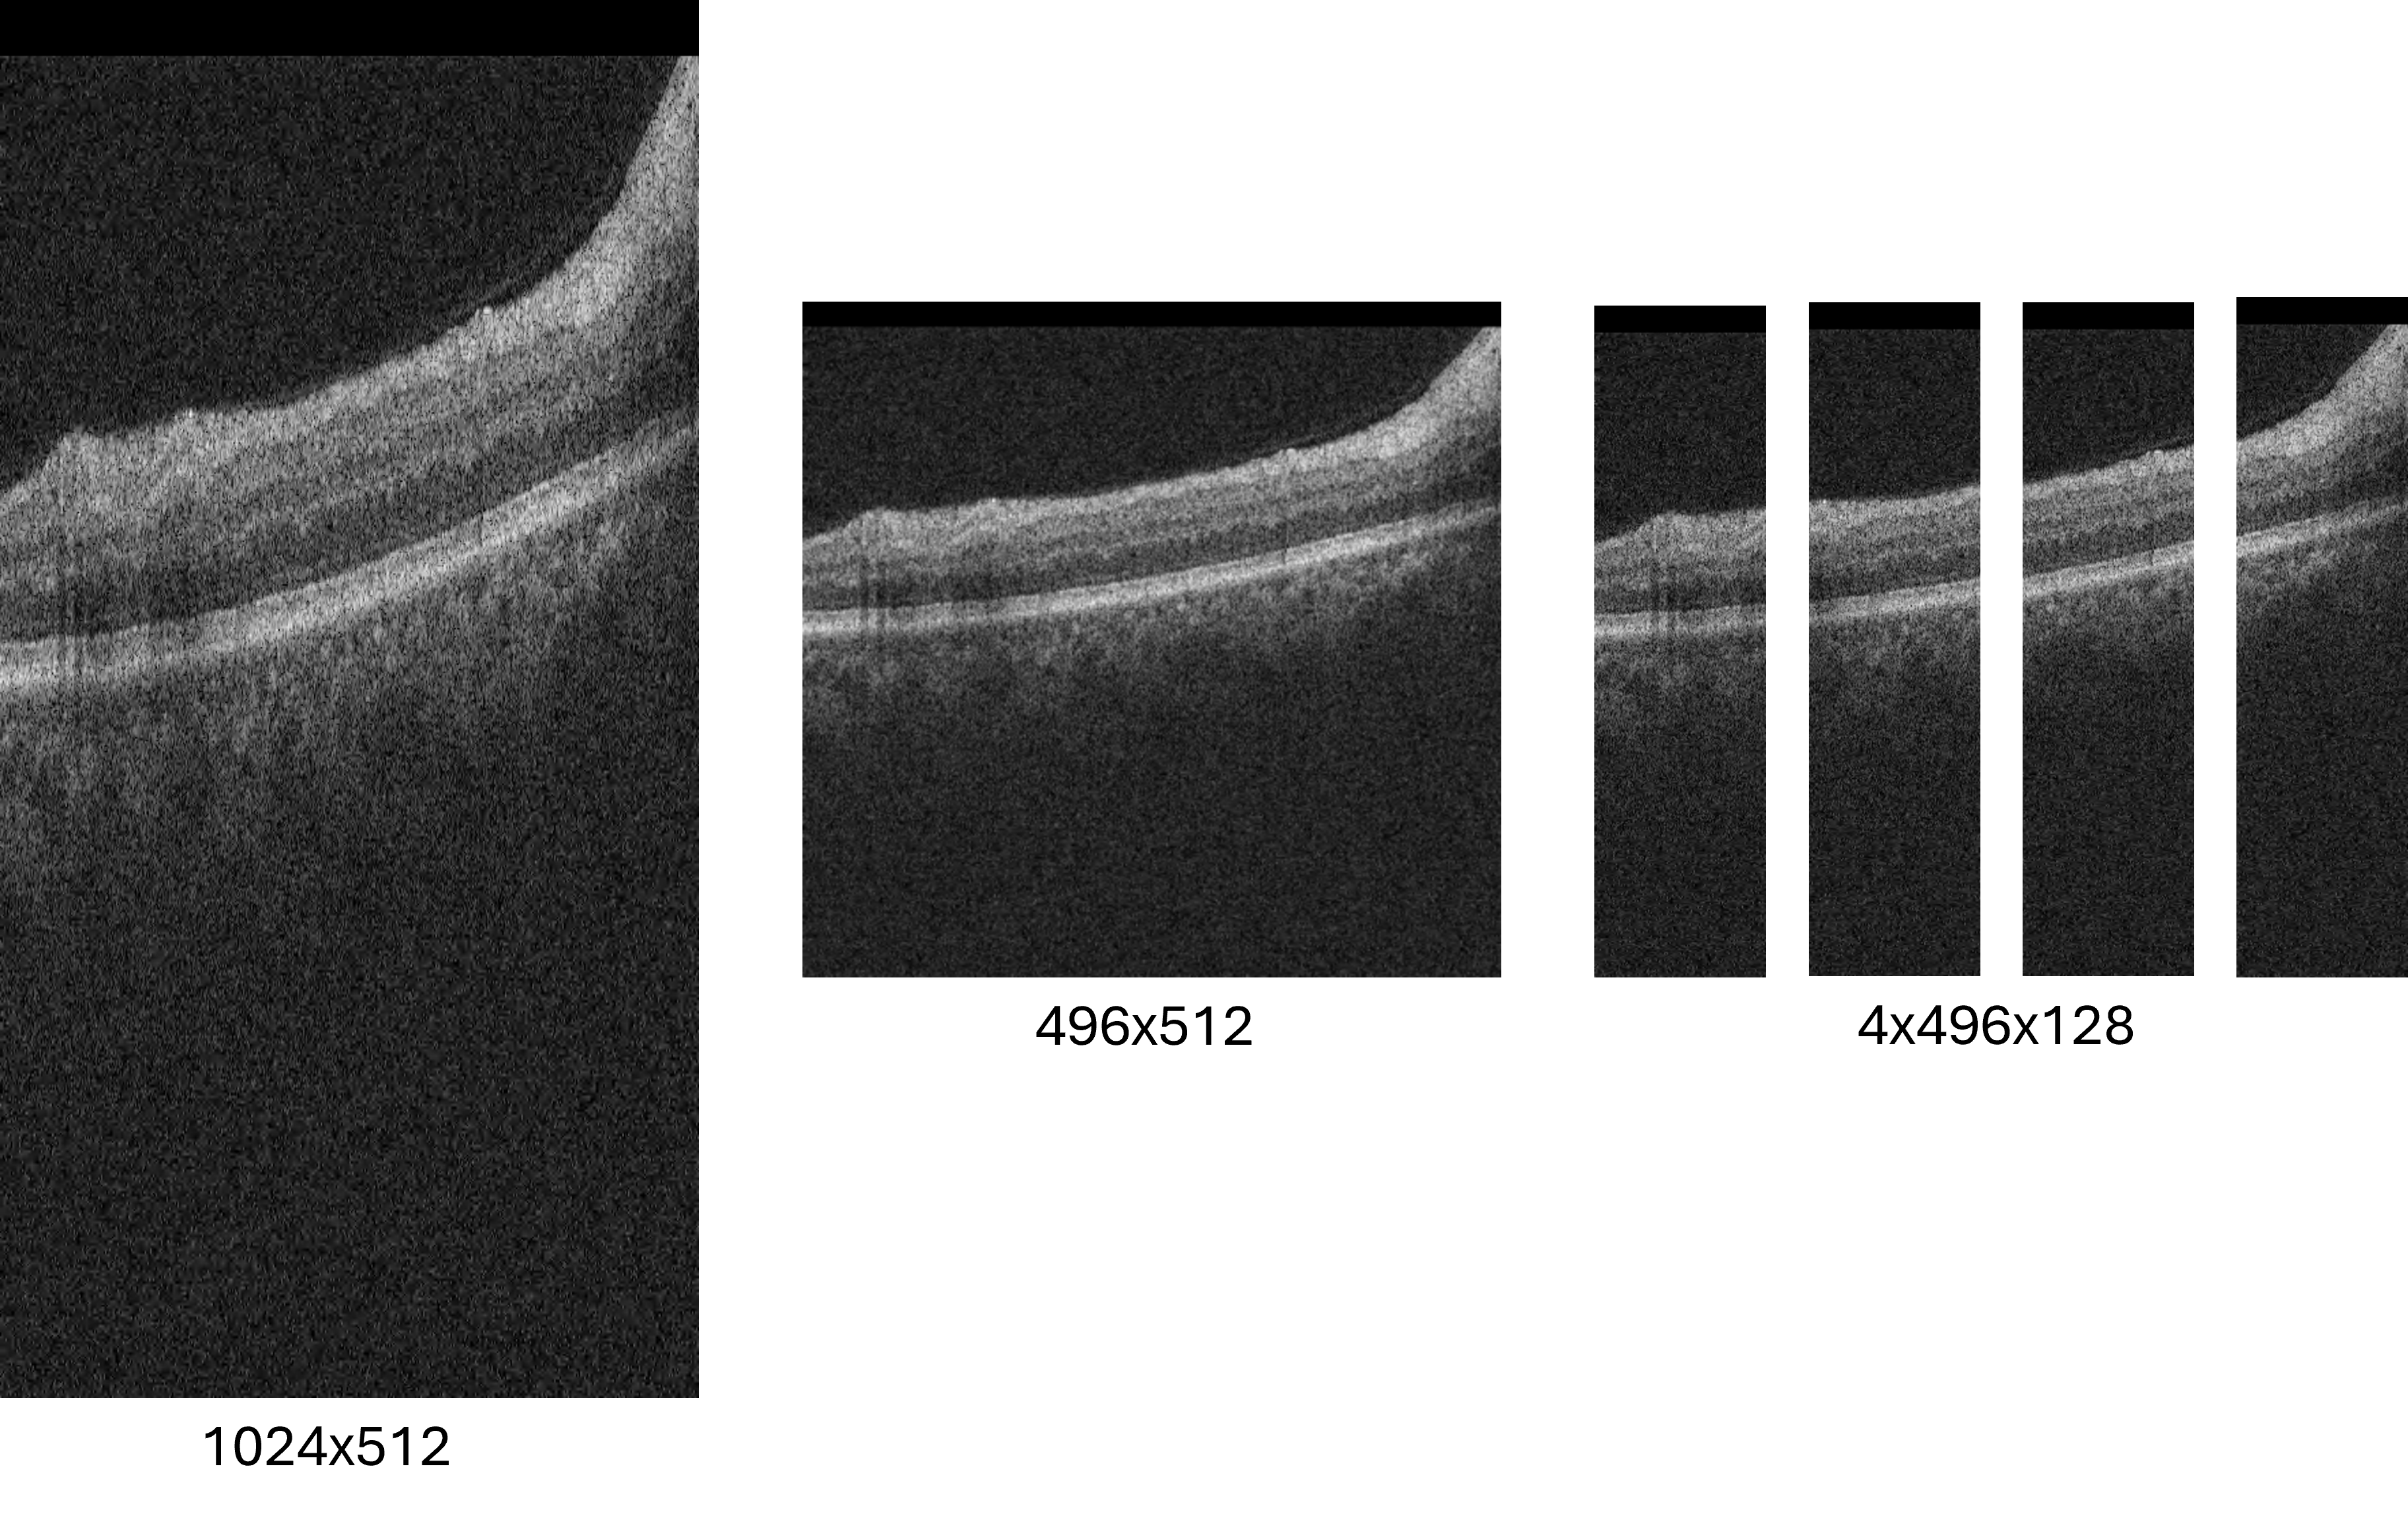
\includegraphics[width=0.65\linewidth]{../figures/CirrusFourPatchExtraction.png}
	\caption{Four vertical patches of shape 496 $\times$ 128 extracted from a Cirrus B-scan.}
	\label{fig:CirrusFourPatchExtraction}
\end{figure}

\begin{figure}[!ht]
	\centering
	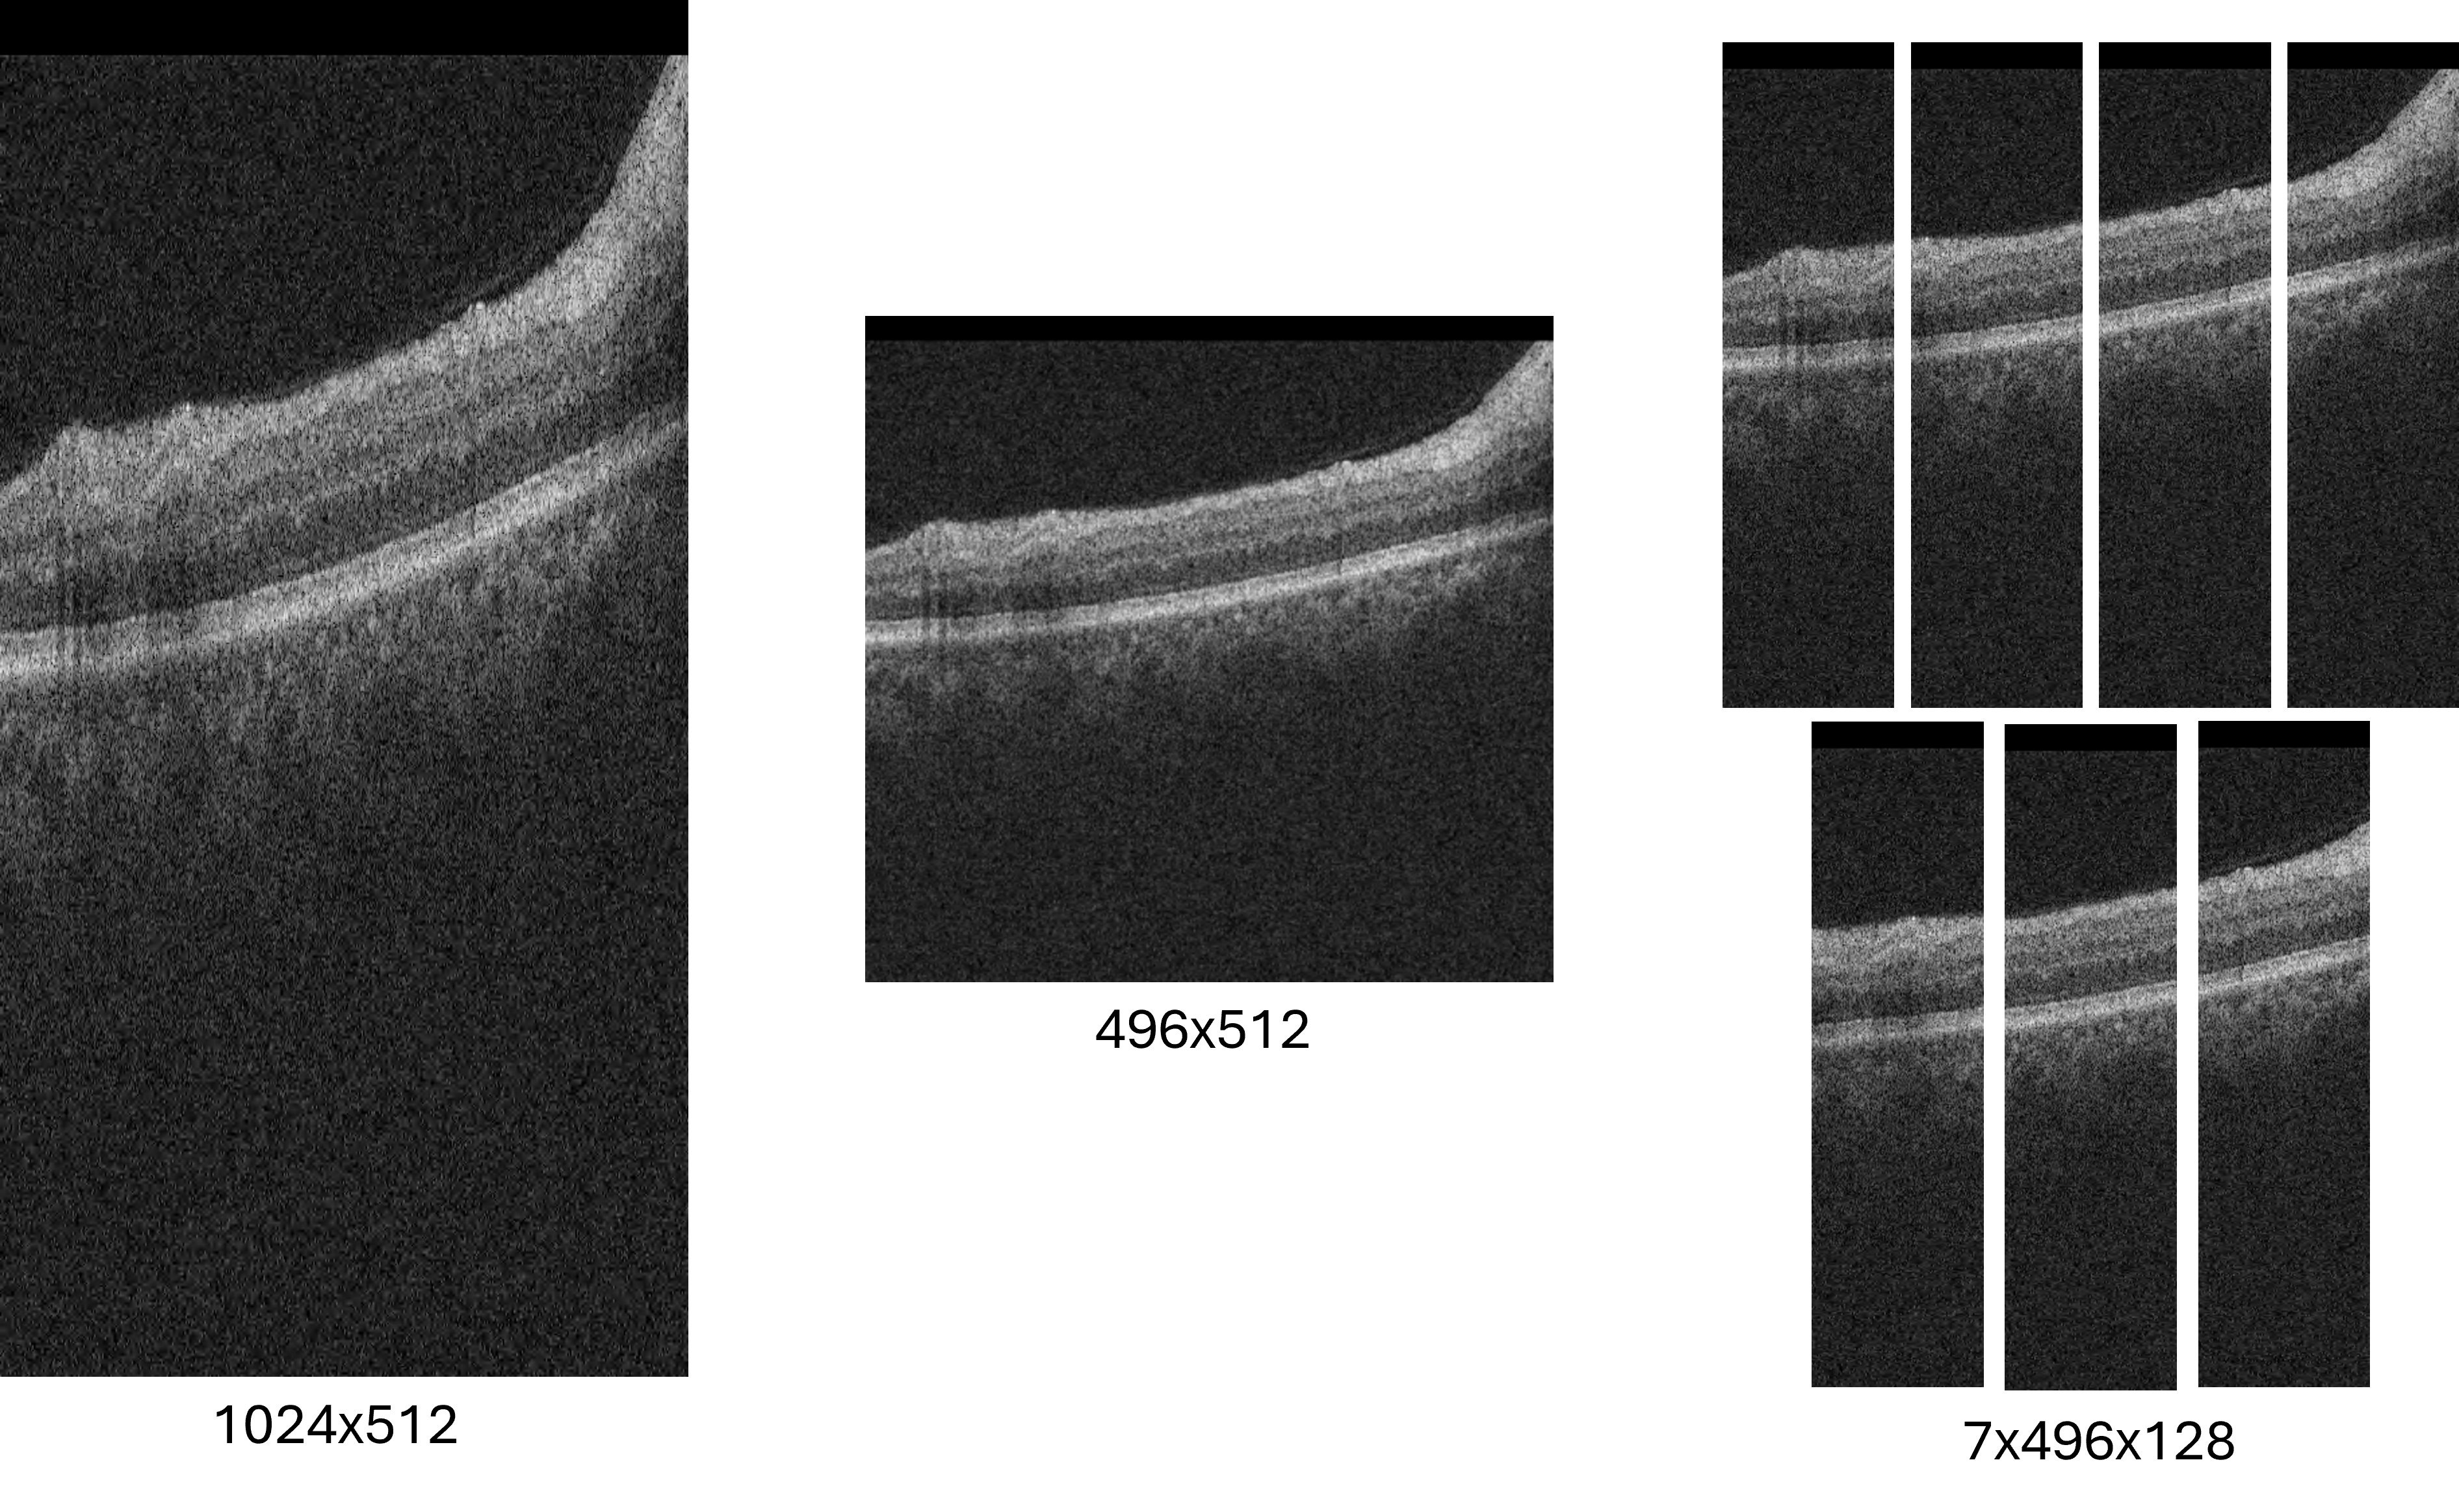
\includegraphics[width=0.65\linewidth]{../figures/CirrusSevenPatchExtraction.png}
	\caption{Seven vertical patches of shape 496 $\times$ 128 extracted from a Cirrus B-scan.}
	\label{fig:CirrusSevenPatchExtraction}
\end{figure}


\begin{figure}[!ht]
	\centering
	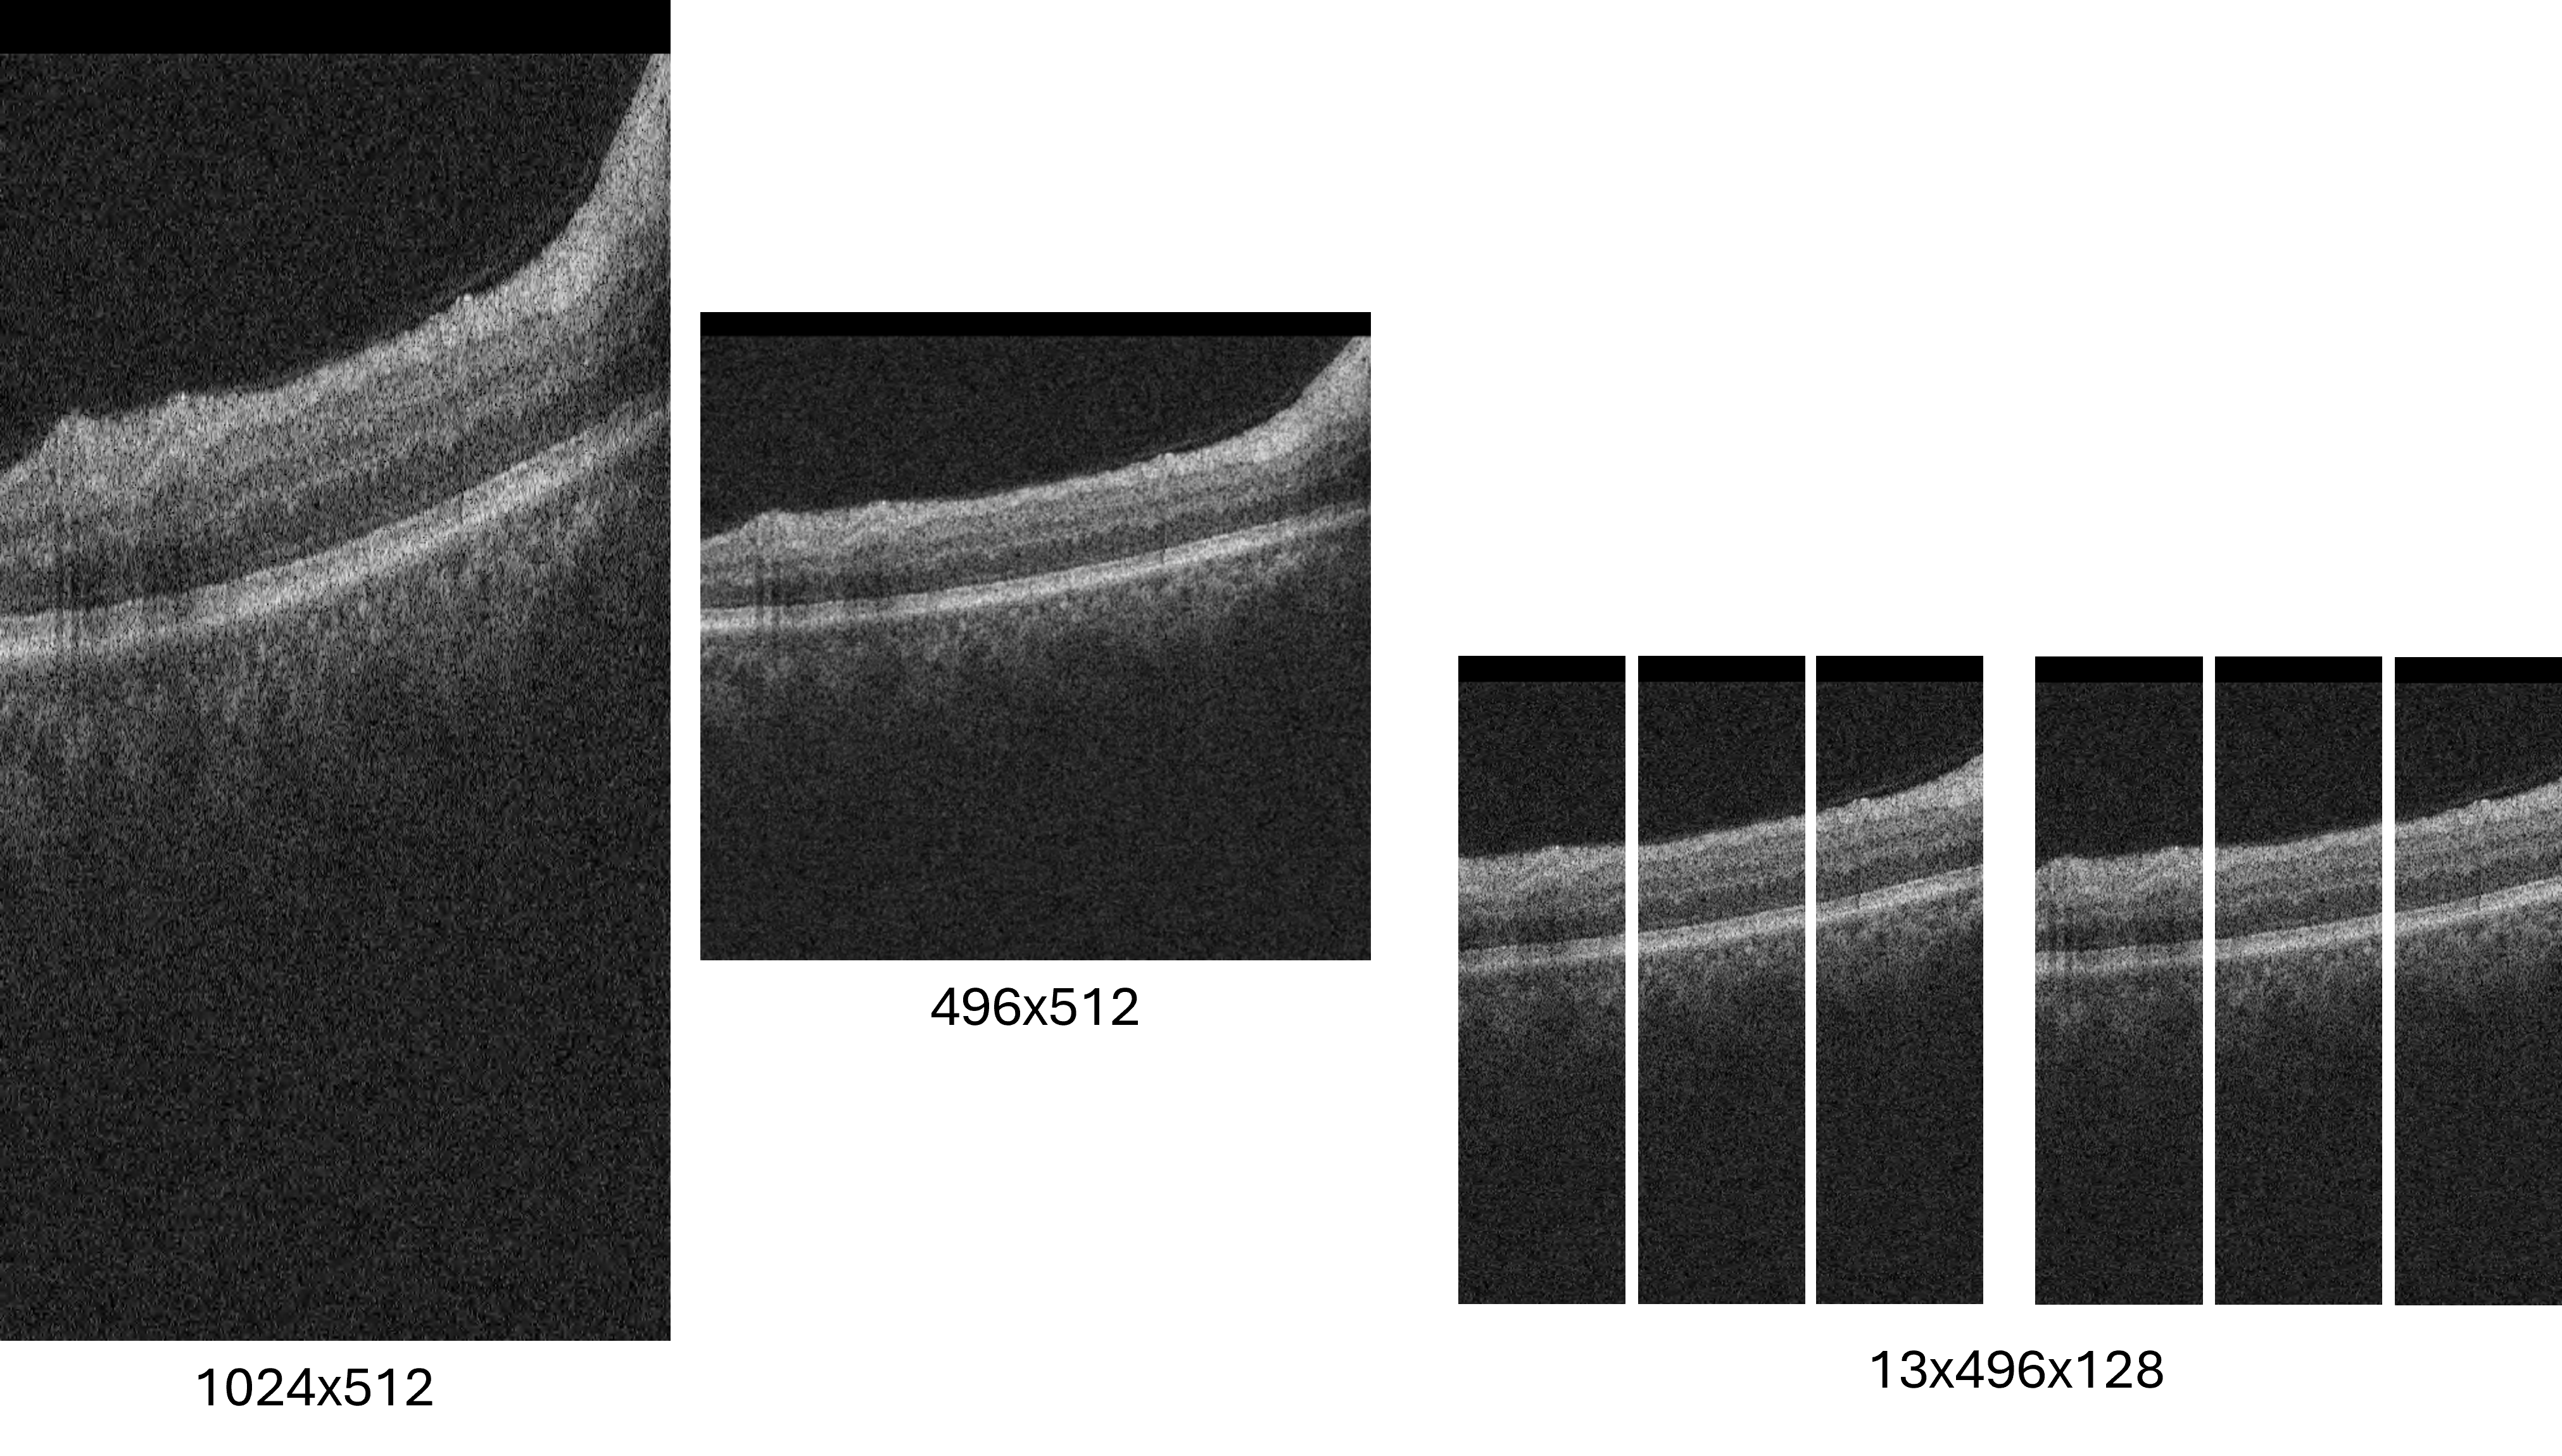
\includegraphics[width=0.75\linewidth]{../figures/CirrusThirteenPatchExtraction.png}
	\caption{Thirteen vertical patches of shape 496 $\times$ 128 extracted from a Cirrus B-scan.}
	\label{fig:CirrusThirteenPatchExtraction}
\end{figure}

When using four vertical patches, the model was trained both for 100 and 200 epochs, maintaining a batch size of 32 and a maximum rotation of $10^{\circ}$, without early stopping. 
\par
Then, the model was trained using seven and thirteen patches for the best and worse performing folds when using four patches, while stopping early in case the validation loss did not progress 25 epochs after the minimum validation loss was encountered. This was used because the model progressed much faster when using seven and thirteen patches per B-scan, as it was trained in a much larger number of images per epoch. Henceforth, it also required more computational power, which further motivated the early stopping.
\par
Using seven vertical patches per image, which was the number of patches that performed best, three different rotations were experimented: no rotation, maximum rotation of $5^{\circ}$, and maximum rotation of $10^{\circ}$. These values were tested for a better understanding of how the rotation of the image affects the segmentation and the model's understanding of anatomic references. The model was trained on a minimum of 100 epochs, after which a patience of 25 epochs was applied. Therefore, if after 100 epochs, the model did not improve its validation loss for 25 consecutive epochs, then training would be interrupted.
\par
Lastly, the model was trained using four patches and a maximum rotation of $5^{\circ}$, using the same early stopping criteria as in the last seven patches runs. This allowed for one last comparison between the two number of patches used in training, under the same conditions. The best model between those trained with four patches and those trained with seven patches was selected to infer on the reserved fold.

\subsubsection{Experiment 2}\label{Experiment2}
The second experiment also involved multi-class segmentation of the retinal fluids. Contrasting with the first experiment, where the segmentation was done using a U-Net, three U-Nets were used in this experiment, one for each fluid. Each U-Net model focused only on the segmentation of one fluid, with one model for IRF, one for SRF, and one for PED.
\par
One of the main problems with multi-class segmentation performed by binary models is the merging of the multiple masks. In this context, multiple fluid classes can be predicted for the same voxel, while only one of those can be correct. In this experiment, two alternatives were explored: order of priority, where the merging of the fluid masks follows a predefined hierarchy that determines which fluid takes precedence, and highest probability, where the assigned class is the one that was predicted with highest probability by its model.
\par
Two different losses were used to regulate the model. Initially, the same loss as the one used in \ref{Experiment1} Experiment 1, with only two classes (background and the fluid that would be segmented), and then, the weighted cross-entropy, using weights that balance the larger quantity of background voxels. This last loss is described in Equation \ref{eq:SegmentationCE}, with $N=2$.
\par
When using the loss from \ref{Experiment1} Experiment 1, each model was trained on two different splits: the split used in the multi-class segmentation experiments and a split created specifically for the segmentation of the fluid that was being segmented. 
\par
The balanced cross-entropy loss was tested on the best performing folds of the multi-class and IRF splits, for the segmentation of IRF, in the same conditions. However, since the results were much worse than those obtained with the initial loss, no more folds or fluids were considered.
\par
All the models were trained with seven vertical patches extracted from each B-scan, on a minimum of 100 epochs, after which a patience of 25 epochs was applied, like what was done in the last runs of \ref{Experiment1} Experiment 1. Similarly, the random transformations applied to the images consisted of horizontal flipping and a maximum rotation of $5^{\circ}$.

\subsection{Intermediate Slice Synthesis}
The objective of the subsequent experiments is to improve the resolution between slices, thus approximating the estimated fluid volume to the true value.
\par
The intermediate slices were generated using the RETOUCH dataset as training and validation data. In this experiment, subvolumes that consist of overlapping triplets of consecutive slices, sampled with a step size of 1, were used, extracted as shown in Figure \ref{fig:FrameInterpolationFramework}. The first and the last slice of these triplets were used for the generation of the middle slice. Consequently, it is possible to evaluate the generated slice in comparison to the original one, as done in other examples of the literature. For each volume, the number of potential subsets is then determined to be $n-2$, where $n$ represents the number of slices within the same volume.

\begin{figure}[!ht]
	\centering
	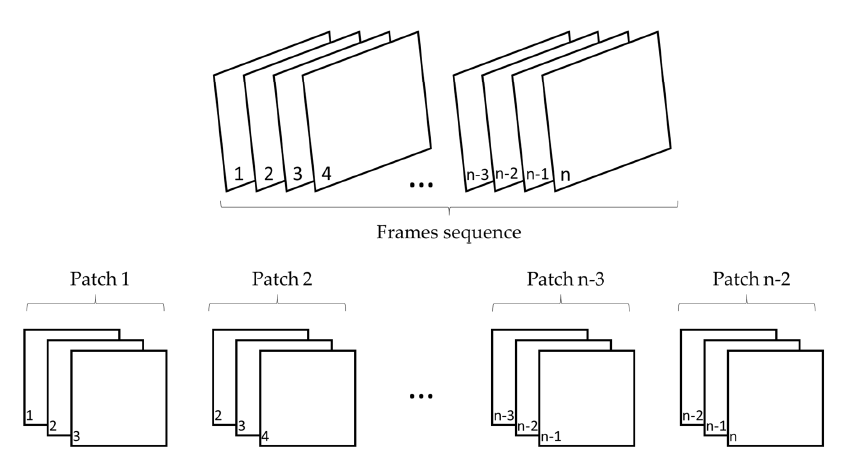
\includegraphics[width=1.0\linewidth]{../figures/FrameInterpolationFramework.png}
	\caption{Scheme explaining the input data of the generative models. Each frame refers to B-scan from an OCT volume. Extracted from \textcite{Tran2020}.}
	\label{fig:FrameInterpolationFramework}
\end{figure}

The generation of slices can be evaluated in specific metrics, as well as through qualitative assessment. To assess the efficacy of the generation model, the model utilized for fluid segmentation could be used for the estimation of the fluid's area in the generated image and to compare the resulting mask with the original image's mask. This comparison can be conducted using the Dice coefficient \parencite{Lopez2023} (see Equation \ref{eq:DiceCoefficientPixels}). However, this metric is insufficient for evaluating the generation performance, as it requires comparisons that encompass the entire slice and not just the fluid region. Examples of such metrics include the mean absolute error (MAE) \parencite{Lopez2023, Wu2022, Zhang2022}, the peak signal-to-noise ratio (PSNR) \parencite{Xia2021, YChen2018, Sanchez2018, Fang2022, Nimitha2024, Kudo2019, You2020, Zhang2024, Zhang2022}, and the structural similarity index measure (SSIM) \parencite{YChen2018, Sanchez2018, Fang2022, Nimitha2024, Kudo2019, You2020, Zhang2024, Zhang2022}.
\par
The MAE and mean squared error (MSE) quantify the errors between the original image and the generated image. For every pixel, the difference between the value in the original image and the generated image is calculated. In MAE, the absolute value of this difference is calculated, and then the mean of all pixels in the image is computed. Meanwhile, in MSE, the difference is squared before computing the mean. In Equation \ref{eq:MAEEquation} and Equation \ref{eq:MSEEquation}, MAE and MSE are described, respectively, where $x_{i}$ is the intensity of the pixel of index $i$ in the predicted image, while $y_{i}$ is the intensity of the pixel with index $i$ in the original image, and $N$ is the number of pixels in the image \parencite{Sara2019, Rajkumar2016}.

\begin{equation}
	\text{MAE} = \frac{1}{N} \sum_{i=1}^{N} |x_i - y_i|
	\label{eq:MAEEquation}
\end{equation}

\begin{equation}
	\text{MSE} = \frac{1}{N} \sum_{i=1}^{N} \left( x_i - y_i \right)^{2}
	\label{eq:MSEEquation}
\end{equation}

PSNR is a metric used to calculate the ratio between the maximum signal power (which corresponds to the maximum value of a pixel in the image) and the power of the distorting noise, which affects the quality of its representation. Therefore, the PSNR, described in Equation \ref{eq:PSNREquation}, is inversely proportional to the mean squared error. PSNR can also be understood as the representation of absolute error in dB \parencite{Sara2019}. It is important to note that in OCT the signal-to-noise ratio is low, due to the speckle present in the images. Therefore, a smaller PSNR is also expected, when compared with other imaging techniques that do not present as much speckle \parencite{Bogunovic2019a}.

\begin{equation}
	\text{PSNR} = 10 \cdot \log_{10} \left( \frac{L^2}{\text{MSE}} \right)
	\label{eq:PSNREquation}
\end{equation}

While the previous metrics focus on the differences between two images at a pixel level, the SSIM is based on the perception of the image. This metric considers the change of perception in structural information, estimating the perceived quality of images and videos. SSIM measures the similarity between the original image and the generated. The SSIM is calculated as shown in Equation \ref{eq:SSIMEquation}, where $x$ and $y$ represent the generated and the original images, respectively, so that $\mu_{x}$ and $\mu_{y}$ are their local means, $\sigma_{x}$ and $\sigma_{y}$ are their standard deviations, while $C_{1}$ and $C_{2}$ are small constants that stabilize the division. The contrast sensitivity (CS) between the images $x$ and $y$ is represented by $CS(x,y)$ \parencite{Sara2019}.

\begin{equation}
	\text{SSIM}(x, y) = \left( \frac{2\mu_x \mu_y + C_1}{\mu_x^2 + \mu_y^2 + C_1} \right) \cdot \left( \frac{2\sigma_{xy} + C_2}{\sigma_x^2 + \sigma_y^2 + C_2} \right) = \left( \frac{2\mu_x \mu_y + C_1}{\mu_x^2 + \mu_y^2 + C_1} \right) \cdot CS(x, y)
	\label{eq:SSIMEquation} 
\end{equation}

Since the best performing models in segmentation resized the images to 496 $\times$ 512, the images were generated to match those dimensions. Therefore, regardless of the device utilized to obtain the OCT volume, all its B-scans were resized to 496 $\times$ 512 for both experiments of image generation.

\subsubsection{Experiment 3}
In the first experiment focused on intermediate slice synthesis, a GAN was used. The underlying principle of a GAN, originally proposed by \textcite{Goodfellow2014}, is based on a competitive game between two networks. The generator network starts with the first and last slice of a subvolume, which is composed of three consecutive B-scans from an OCT scan, and aims to generate the intermediate slice. In contrast, the discriminator network is trained to distinguish between the generated and real slices. When the discriminator correctly labels generated slices as fake, the generator is penalized, motivating it to fool the discriminator and consequently improving its generation, resulting in outputs more similar to the real inputs. However, the discriminator network loss also penalizes misclassifications, dependent on the probability of the prediction. As a result, as the generator improves, so does the discriminator \parencite{Goodfellow2020}. The overall framework for GANs is illustrated in Figure \ref{fig:GANFramework}.

\begin{figure}[!ht]
	\centering
	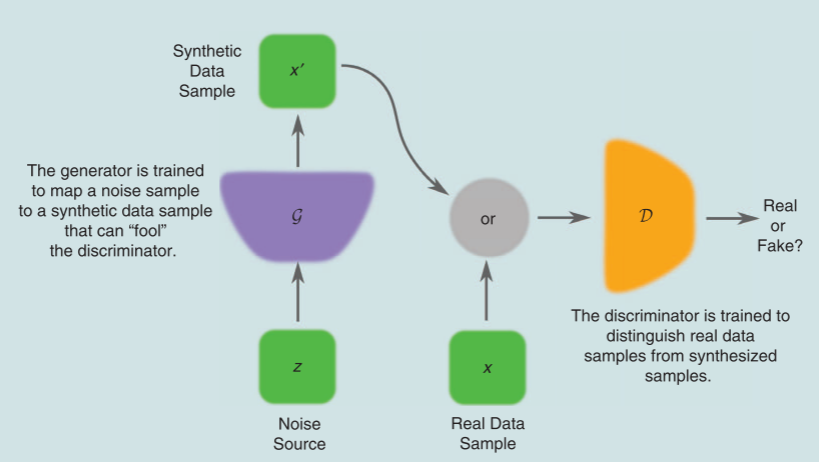
\includegraphics[width=0.7\linewidth]{../figures/GANFramework}
	\caption{Example of a GAN framework, where $\mathcal{D}$ is the discriminator and $\mathcal{G}$ is the generator \cite{Creswell2018}.}
	\label{fig:GANFramework}
\end{figure}

The GAN implemented by \textcite{Tran2020} was used to generate the intermediate slices of the OCT volumes. This framework is used in the interpolation of intermediate slices in video and is trained in patches of 64 $\times$ 64.
\par
In the original implementation, one patch is randomly extracted from the triplet of images and used in training. Due to the much smaller quantity of data available in OCT, all the possible disjoint 64 $\times$ 64 patches were extracted from each B-scan. The extraction was done from top to bottom and in the last row of slices, the image was padded until it had 64 pixels. An example of the patches extracted from a Cirrus B-scan can be seen in Figure \ref{fig:CirrusSixtyFourPatchExtraction}. By methodically extracting the patches, triplets are easily created by accessing patches of the same index in the three consecutive images.

\begin{figure}[!ht]
	\centering
	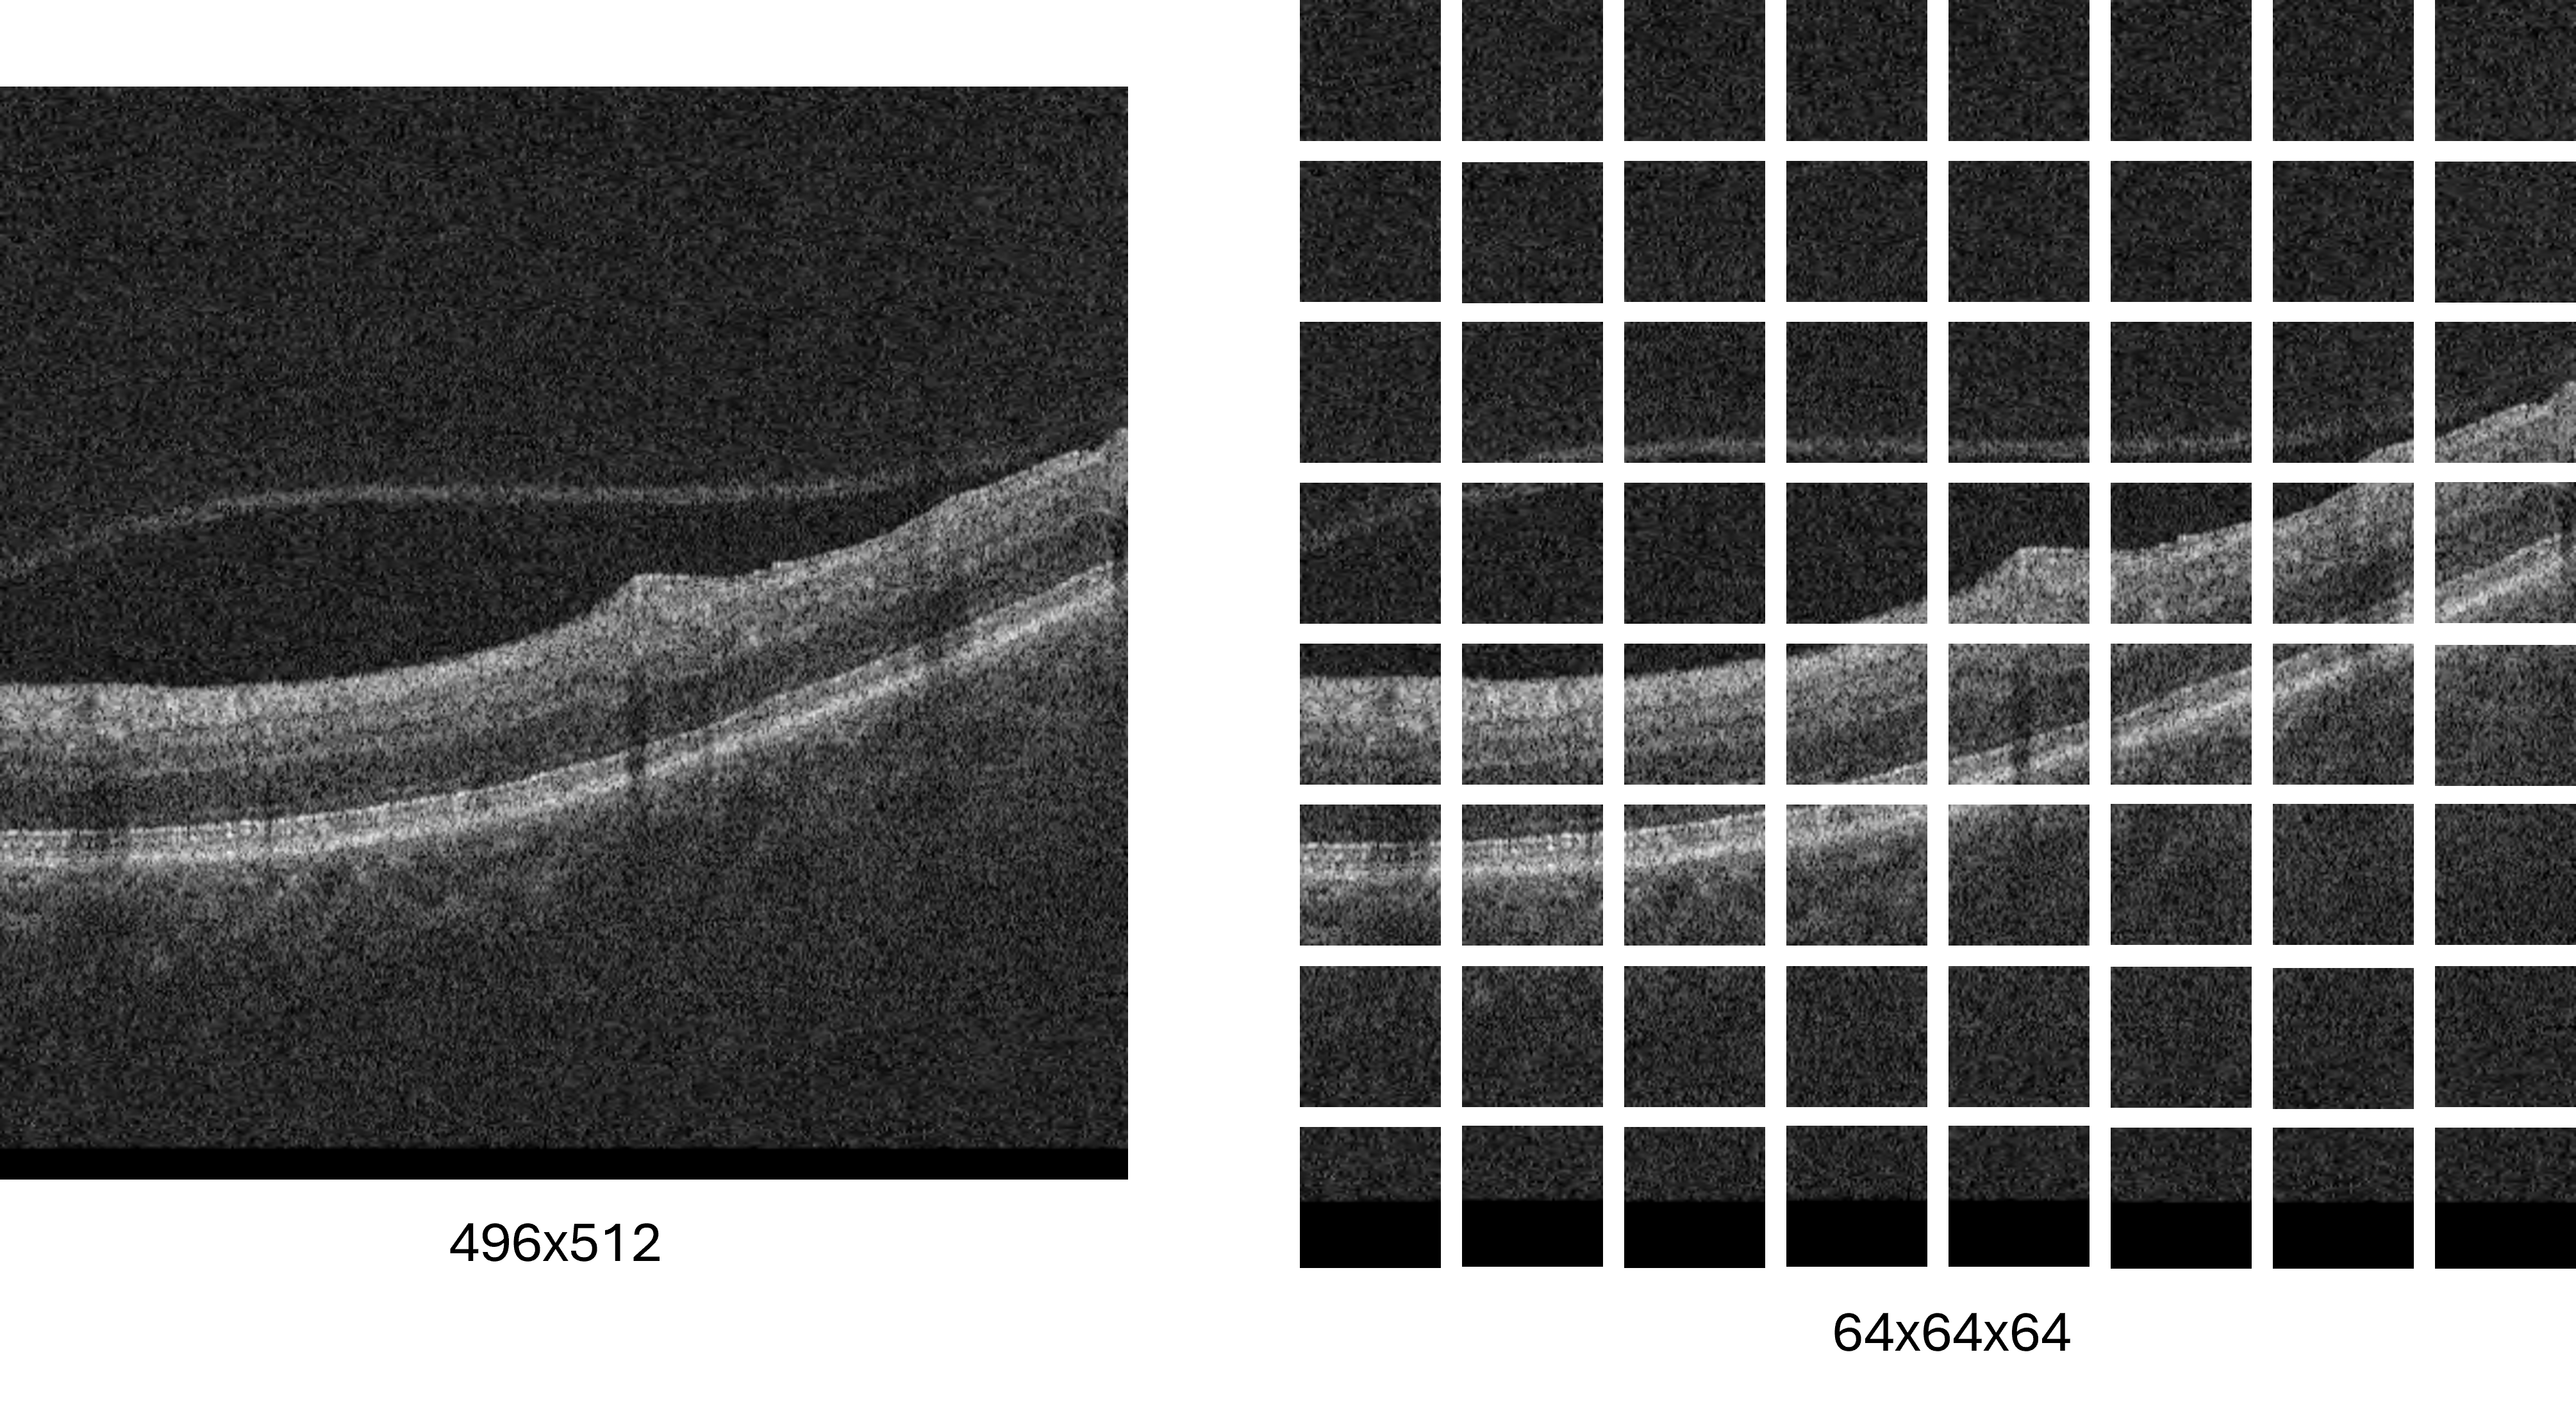
\includegraphics[width=0.7\linewidth]{../figures/CirrusSixtyFourPatchExtraction.png}
	\caption{Patches with shape 64 $\times$ 64 extracted from a Cirrus B-scan which was resized to 496 $\times$ 512.}
	\label{fig:CirrusSixtyFourPatchExtraction}
\end{figure}

The generator of the GAN is composed of contracting and expanding path. In the contracting path, convolutions are applied to the images and feature maps, followed by batch normalization, and a leaky ReLU activation function. After the images are downsampled to 512 $\times$ 8 $\times$ 8, reaching the bottleneck, the expanding path begins, where deconvolutions are applied, followed by batch normalization, and a leaky ReLU. Finally, after the last deconvolution, the hyperbolic tangent function is used as the final activation function, resulting in an output of size 64 $\times$ 64, in range -1 to 1. An illustrative scheme of the generator can be seen in Figure \ref{fig:GeneratorArchitecture}.

\begin{figure}
	\centering
	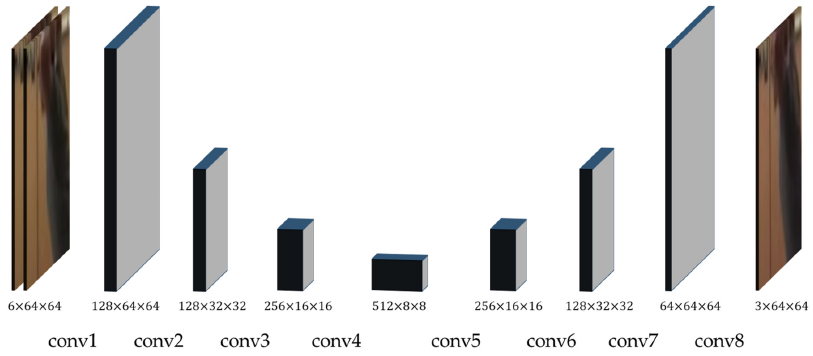
\includegraphics[width=1.0\linewidth]{figures/GeneratorArchitecture}
	\caption{Architecture of the generator used in the GAN. It has a contracting and an expanding path, making it a U-Net like network \parencite{Tran2020}.}
	\label{fig:GeneratorArchitecture}
\end{figure}


To match the needs of our application, some changes had to be made in the generator regarding the input shape. As shown in Figure \ref{fig:GeneratorArchitecture}, the input has six channels, one red, one green, and one blue (RGB) for each input patch. Similarly, the output has three channels, for the generated middle patch. In our application, each patch in the input only had one channel, since the OCT B-scans are images in gray scale, instead of RGB, as in the original implementation. Therefore, the output only had one channel. 
\par
The final activation function, the hyperbolic tangent, outputs values between -1 and 1. Since the output images were compared to images in range 0 to 1, the final activation function was changed to the sigmoid. This function converts the values output from the last convolution to the range of 0 to 1, where it can be compared to the GT images.
\par
The GAN's discriminator receives as input a patch of shape 64 $\times$ 64, and outputs a probability of the input patch being real. The discriminator is composed of five consecutive convolutions. The first convolution is followed by a leaky ReLU activation function. The second, third, and fourth convolutions are followed by a batch normalization and a leaky ReLU activation function. After the last convolution, the sigmoid is applied and converts the final output to a value between 0 and 1 that represents the probability of the image being real. In Table \ref{tab:GeneratorDiscriminatorArchitecture}, the layers that compose the discriminator and the generator are explained, including the shape of the outputs.

\begin{table*}[!ht]
	\setlength{\tabcolsep}{6pt}
	\renewcommand{\arraystretch}{1.3}
	\caption{Layers that compose the generator and the discriminator. Each convolution is represented by Conv2d(K, OC, S), where K is the kernel size, OC is the number of output channels, and S is the stride. The same notation is used in deconvolutions, represented by TransposedConv2d. The output size is shown following C $\times$ H $\times$ W notation, where C is the number of channels, H is the height, and W is the width. The inputs have shape $1 \times 64 \times 64$. Adapted from \textcite{Tran2020}.}
	\centering
	\resizebox{\textwidth}{!}{\begin{tabular}{c c c}
		\hline
		\hline
		\multicolumn{3}{c}{\textbf{Generator}} \\
		\hline
		\textbf{Layers} & \textbf{Details} & \textbf{Output Size (C $\times$ H $\times$ W)} \\
		\hline
		\textbf{1} & Conv2d(3, 128, 1), BatchNorm2d, LeakyReLU & 128 $\times$ 64 $\times$ 64 \\
		\textbf{2} & Conv2d(4, 128, 2), BatchNorm2d, LeakyReLU & 128 $\times$ 32 $\times$ 32 \\
		\textbf{3} & Conv2d(4, 256, 2), BatchNorm2d, LeakyReLU & 256 $\times$ 16 $\times$ 16 \\
		\textbf{4} & Conv2d(4, 512, 2), BatchNorm2d, LeakyReLU & 512 $\times$ 8 $\times$ 8 \\
		\textbf{5} & TransposedConv2d(4, 256, 2), BatchNorm2d, LeakyReLU & 256 $\times$ 16 $\times$ 16 \\
		\textbf{6} & TransposedConv2d(4, 128, 2), BatchNorm2d, LeakyReLU & 128 $\times$ 32 $\times$ 32 \\
		\textbf{7} & TransposedConv2d(4, 64, 2), BatchNorm2d, LeakyReLU & 64 $\times$ 64 $\times$ 64 \\
		\textbf{8} & TransposedConv2d(1, 1, 1), Sigmoid & 1 $\times$ 64 $\times$ 64 \\
		\hline
		\hline
		\multicolumn{3}{c}{\textbf{Discriminator}} \\
		\hline
		\textbf{Layers} & \textbf{Details} & \textbf{Output Size (C $\times$ H $\times$ W)} \\
		\hline
		\textbf{1} & Conv2d(4, 64, 2), LeakyReLU & 64 $\times$ 32 $\times$ 32 \\
		\textbf{2} & Conv2d(4, 128, 2), BatchNorm2d, LeakyReLU & 128 $\times$ 16 $\times$ 16 \\
		\textbf{3} & Conv2d(4, 256, 2), BatchNorm2d, LeakyReLU & 256 $\times$ 8 $\times$ 8 \\
		\textbf{4} & Conv2d(4, 512, 2), BatchNorm2d, LeakyReLU & 512 $\times$ 4 $\times$ 4 \\
		\textbf{5} & Conv2d(4, 1, 1), Sigmoid & 1 $\times$ 1 $\times$ 1 \\
		\hline
		\hline
	\end{tabular}}
	\label{tab:GeneratorDiscriminatorArchitecture}
\end{table*}

In the training of a GAN, both the generator and the discriminator are being trained sequentially and independently. First, the generator, which receives the previous and following patch of the input triplet, attempts to generate the intermediate patch. The generated image is then compared to the original image, using the generator loss, which is then used in the updating of the generator weights. The generator loss is composed of four components: the adversarial, the MAE, the multi-scale SSIM (MS-SSIM), and the gradient difference loss (GDL). The overall loss function is described in Equation \ref{eq:GeneratorLoss}, where $\lambda_{\text{adv}}=0.05$, $\lambda_{\text{MAE}}=1.0$, $\lambda_{\text{MS-SSIM}}=6.0$, and $\lambda_{\text{GDL}}=1.0$, representing the weights of each loss component.

\begin{equation}
	\mathcal{L}_{\text{Gen}} = \lambda_{\text{adv}} \times \mathcal{L}_{\text{adv}} + \lambda_{\text{MAE}} \times \mathcal{L}_{\text{MAE}} + \lambda_{\text{MS-SSIM}} \times \mathcal{L}_{\text{MS-SSIM}} + \lambda_{\text{GDL}} \times \mathcal{L}_{\text{GDL}}
	\label{eq:GeneratorLoss}
\end{equation}

The adversarial loss is used in the evaluation of how good the output from the generator fools the discriminator. This evaluation is done using the binary cross-entropy (BCE). To calculate this, the generated image is input into the discriminator, which then outputs the probability of being real. Afterwards, the BCE is calculated for the predicted probability and 1, the label of a real image. The better the generator fools the discriminator, the closer the output of the discriminator is to one, and, therefore, the closer the adversarial loss is to 0. The adversarial loss is explained in Equation \ref{eq:AdversarialLoss}, where $\mathcal{D}$ is the discriminator, $x$ is the generated image, and $y$ is the label that indicates that the image is real. It is important to note that in the generator training, the images that are input to the discriminator are detached, not contributing to the updating of the discriminator weights in this step.

\begin{equation}
	\mathcal{L}_{\text{adv}} (\mathcal{D}(x), y) = \mathcal{L}_{\text{BCE}} (\mathcal{D}(x), y) = - \left[ y \text{log}(\mathcal{D}(x)) + (1 - y)\text{log}(1 - \mathcal{D}(x)) \right]
	\label{eq:AdversarialLoss}
\end{equation}

The MAE loss, also referred to as $L_{1}$ loss, performs a pixel-by-pixel comparison between the generated image, $x$, and the real image, $y$, as described in Equation \ref{eq:MAEEquation}, where $i$ is the index of a pixel. While this loss gives an insight of how similar the images are, on average, this loss can be deceiving, since the model can blur the output to attain better MAE values. For this reason, this loss must be combined with other reconstructive losses, such as the MS-SSIM and the GDL.
\par
The MS-SSIM loss seeks to preserve the structural similarity, at different scales, between the real and the generated image, facilitating a smoother output. This loss, originally suggested by \textcite{Wang2003}, is described in Equation \ref{eq:MSSSIMLoss}, while the MS-SSIM used in this implementation is explained in Equation \ref{eq:MSSSIM}, using the concepts of SSIM and CS explained in Equation \ref{eq:SSIMEquation}. This version of the MS-SSIM is faster than the original implementation \parencite{Wang2003}, while using the same array of weights $\beta$ and number of levels $M$, which is set to 5. Therefore, the MS-SSIM corresponds to the product of the contrast sensitivity in the image for first four levels and the SSIM of the image in the last level, all raised to the power of the respective level's weights.

\begin{equation}
	\mathcal{L}_{\text{MS-SSIM}} (x, y) = 1 - \text{MS-SSIM}(x, y)
	\label{eq:MSSSIMLoss}
\end{equation}

\begin{equation}
	\text{MS-SSIM}(x, y) = \prod_{j=1}^{M-1} \left[ \text{CS}_j(x, y) \right]^{\beta_j} \cdot \left[ \text{SSIM}_M(x, y) \right]^{\beta_M}
	\label{eq:MSSSIM}
\end{equation}

The last component of the loss is the GDL, proposed originally by \textcite{Mathieu2016}. This component is used to reduce the motion blur in the generated images, a problem in video datasets. In this loss, the relative difference of neighboring pixels between the generated and true images is considered, as shown in Equation \ref{eq:GDLLoss}. In this equation, $i$ and $j$ are the index of row and column, respectively, that identify a pixel of the image, with $\alpha$ set to 2.

\begin{equation}
	\mathcal{L}_{\text{GDL}}(x, y) = \sum_{i,j} \left( \left|\,|x_{i,j} - x_{i-1,j}| - |y_{i,j} - y_{i-1,j}|\,\right|^{\alpha} + \left|\,|x_{i,j} - x_{i,j-1}| - |y_{i,j} - y_{i,j-1}|\,\right|^{\alpha} \right)
	\label{eq:GDLLoss}
\end{equation}

After the images are generated and evaluated using the previously defined generator loss, two images are input, subsequently, to the discriminator, with one of them being fake while the other is real. The discriminator outputs the probability of each image being real and its result is compared to the true label of each image using the BCE. The BCE is calculated for the probabilities predicted by the discriminator and the image's respective label as described in Equation \ref{eq:AdversarialLoss}. This is done for the fake image and for the real image. The mean between the BCE calculated for the fake image and the BCE computed for the real image is the discriminator loss.
\par
The GAN was trained in 250 epochs, using a batch size of 32 and $2 \times 10^{-4}$ as the learning rate. The selected optimizer was Adam, with $\beta_{1}=0.5$ and $\beta_{2}=0.999$.

\subsubsection{Experiment 4}
As in the previous experiment, the intermediate slice was generated using the first and last slices of a subvolume that consists of three consecutive B-scans from an OCT scan. However, in this experiment, inspired by the work of \textcite{Nishimoto2024}, the intermediate slice was generated using a U-Net. While the U-Net is more commonly applied in segmentation, as seen in the reviewed literature, \textcite{Nishimoto2024} apply it to generate the intermediate slices of a subvolume. The U-Net receives the edge slices as input and forces the output of the intermediate ones. In the paper \parencite{Nishimoto2024}, this was tested for three, four, and five slices. However, in this experiment it was utilized to generate a single intermediate slice.
\par
In this experiment, the whole image is input to the network and for that reason the batch size was set to 8. The optimizer utilized was Adam with a learning rate of $2 \times 10^{-4}$ and the model was trained for 200 epochs.

\subsection{Fluid Volume Estimation}
The estimation of fluid volume was done using the optimal segmentation and intermediate slice generation models. The GAN was used in the generation of the intermediate slices in the OCT volumes, while the best performing multi-class segmentation U-Net model inferred the segmentation masks to both the unaltered volumes and the volumes with generated slices. 
\par
The OCT scans used in the fluid volume estimation experiments were the ones from the \hbox{RETOUCH} dataset that composed the reserved fold in the segmentation and generation experiments and the ones from the private dataset obtained in Hospital São João. These volumes were selected because no model was trained or validated on them, allowing an insight of both models generalization on unseen data and how the increase in resolution affects the total fluid volume.
\par
The area of each fluid in each OCT scan was estimated considering the resolution of each OCT scan, which varies according to the device utilized to obtain the OCT volume. Afterwards, the area is multiplied by the axial distance (half the axial distance to the previous slice plus half the axial distance to the following slice) to obtain the volume of fluid per slice. In the first and last slice of an OCT volume, the area is multiplied by half of the axial distance (half the axial distance to the neighboring slice). The total volume of fluid in an OCT scan can be estimated by summing the fluid volumes of all individual B-scans. This allows the volume estimation of IRF, SRF, and PED, as well as the overall fluid volume in the OCT scan.
\par
The total volume of fluid from class $c$ in a slice of index $s$ is defined in Equation \ref{eq:FluidEstimationSlice}. The slice belongs to an OCT volume obtained using device $D$ and its total number of B-scans is defined as $S$. In this equation, $H_{D}$ and $W_{D}$ are the height and width of a voxel, respectively, obtained with device $D$, while $d_{D,s,s+1}$ is the axial distance between the slice of index $s$ and the slice of index $s+1$, a value that depends on the device $D$ characteristics. The variable $l_{i}$ is the label attributed to the voxel of index $i$. Like the variable $c$, $l$ can be one of the following classes: $\{0,1,2,3\}$, which respectively correspond to background, IRF, SRF, and PED. Meanwhile, the total volume of fluid from a class $c$ in an OCT scan obtained with device $D$ is described by Equation \ref{eq:FluidEstimationVolume}, and consists of the sum of the fluid's volume obtained in each B-scan that compose the OCT.

\begin{equation}
	\begin{aligned}
		f_{c,s,D} &= \sum_{i} \left( v_{i,s,D} \times y_{i,c} \right) \quad \text{where: }\\
		v_{i,s,D} &=
		\begin{cases}
			0.5 \times H_{D} \times W_{D} \times d_{D,s,s+1} & \text{if $s=0$}\\
			0.5 \times H_{D} \times W_{D} \times d_{D,s,s-1} & \text{if $s=S$}\\
			0.5 \times H_{D} \times W_{D} \times d_{D,s,s-1} + 0.5 \times H_{D} \times W_{D} \times d_{D,s,s+1} & 
			\text{otherwise}\\
		\end{cases}\\
		y_{i,c} &=
		\begin{cases}
			1 &\text{if } l_{i} = c\\
			0 &\text{if } l_{i} \neq c\\
		\end{cases} 
		\label{eq:FluidEstimationSlice}
	\end{aligned}
\end{equation}

\begin{equation}
	F_{c,D} = \sum_{s}^{S} f_{c,s,D}
	\label{eq:FluidEstimationVolume}
\end{equation}

The fluid volumes resulting from both experiments were compared. Since there is no true value for the fluid quantity in the OCT scans, the results were compared with each other. Therefore, the results would be deemed satisfying in case they do not vary more than an order of magnitude between each other. In case a significant difference was observed, the generated images and their respective masks were analyzed, in order to understand what is causing the observed difference between experiments.

\subsubsection{Experiment 5}
In this experiment, the fluid volumes were calculated for the OCT scans without the generated slices. The best segmentation model was utilized to segment the fluid in three classes and the volume was estimated for each class as described. The results from this experiment allow the comparison with the values obtained in the following experiment, where slice generation was used.

\subsubsection{Experiment 6}
This experiment consisted of the fluid volume estimation in OCT scans with generated images. The model used in segmentation was the same as in the previous experiment, which predicted the fluid masks for all the slices. From the predicted fluid masks, the fluid volume was estimated and compared with those obtained in the previous experiment. 
\chapter{Experiments}\label{Experiments}
Building upon the methods and materials exposed, the experiments conducted during this dissertation are explained in depth in this chapter. It begins with a description of how the data were split, followed by the experiments on fluid segmentation, intermediate slice generation, and fluid volume estimation.
\par
All experiments were conducted using an NVIDIA GeForce RTX 3080 GPU and the \hbox{PyTorch} machine learning library (version 2.5.1).

\section{Data Partition}\label{CrossValidation}
To promote consistency across all experiments, the conditions were held identical. In every experiment, the data were split into five folds, with different splits being used for the segmentation and generation tasks. From these five folds, one was reserved until the end to compare the performance of the models trained in the different experiments and identify the one that generalizes best to an unseen image set. The remaining four folds were used for training the models through a 4-fold cross-validation procedure, in which three folds were used for training and one for validation. Therefore, four training runs are completed in each experiment, rotating the validation fold across runs. The reserved fold consists of the same OCT volumes for all experiments, allowing for further comparisons on data not seen by any of the models. Fold 1 was randomly selected as the reserved fold.
\par
For the multi-class segmentation models, the data were split so that the quantity of each fluid and the number of volumes per vendor were evenly distributed across the folds - referred to as a multi-class 5-fold split. This balanced distribution allows for a fairer assessment of the model's learning ability and its performance on data with varying characteristics (e.g., from different vendors). To achieve this, a custom algorithm was developed to divide the data into five folds while minimizing discrepancies in fluid distribution and the number of slices per vendor within each fold.
\par
A possible distribution of the 70 OCT volumes from the RETOUCH dataset, which were used in the training of the fluid segmentation models, can be seen in Table \ref{tab:FiveFoldSplit}. The split was applied to the volumes and not to the slices. Slices from the same volume must be kept together to prevent data leakage, where similar images obtained from the same patient appear in both the training and validation sets, potentially resulting in overly optimistic performance metrics.

\begin{table*}[!ht]
	\setlength{\tabcolsep}{6pt}
	\renewcommand{\arraystretch}{1.3}
	\caption{Number of OCT volumes per vendor in each fold, considering a 5-fold split.}
	\centering
	\begin{tabular}{|c|c|c|c|c|c|}
		\hline
		\textbf{Vendors} & \textbf{1$^{st}$} & \textbf{2$^{nd}$} & \textbf{3$^{rd}$} & \textbf{4$^{th}$} & \textbf{5$^{th}$} \\
		\hline
		\textbf{Cirrus} & 5 & 5 & 5 & 5 & 4 \\
		\textbf{Spectralis} & 5 & 5 & 5 & 5 & 4 \\
		\textbf{Topcon} & 4$^{a}$ + 1$^{b}$ & 4$^{a}$ + 1$^{b}$ & 4$^{a}$ & 4$^{a}$ & 4$^{a}$ \\
		\hline
		\multicolumn{6}{l}{Volumes marked with \textbf{\textit{a}} consist of 128 B-scans.} \\
		\multicolumn{6}{l}{Volumes marked with \textbf{\textit{b}} consist of 64 B-scans.} \\
	\end{tabular}
	\label{tab:FiveFoldSplit}
\end{table*}

For experiments using a binary segmentation approach, the volumes can be redistributed using the same algorithm, but with fewer constrains - a fluid-specific 5-fold split. In this case, the folds are created based only on the vendor and amount of the target fluid, thus eliminating the restrictions imposed by the quantities of the other two fluids. Nevertheless, the volumes that are in the previously defined reserved fold must not be used in either training in validation.
\par
For the experiments related with inter-slice generation, the 5-fold split of the data was not done by considering the quantity of fluid in each fold. Since the test volumes of the RETOUCH dataset were used in this experiment and fluid masks are not available, the quantity of fluid in each test volume is unknown. Please note that, for comparison purposes, one of the folds in this 5-fold split is the one reserved in the multi-class segmentation split for testing.
\par
The split was performed by taking into consideration solely the number of slices per device. In these experiments, the characteristics of each device are important, since each device has a specific inter-slice distance. This distance varies even across devices from the same vendor and is an important factor in image generation.
\par
Considering both training and testing volumes of the RETOUCH dataset, there are 38 Cirrus, 38 Spectralis, 13 Topcon T-1000, and 23 Topcon T-2000 (two of which with 64 slices). The fold reserved in the multi-class segmentation task for testing is composed of the following volumes: 4 Cirrus, 5 Spectralis, 3 Topcon T-1000, and 2 Topcon T-2000 (one of which with 64 slices). The volumes remaining for the four folds used in the generation task are distributed as shown in Table \ref{tab:FourFoldSplit}.

\begin{table*}[!ht]
	\setlength{\tabcolsep}{6pt}
	\renewcommand{\arraystretch}{1.3}
	\caption{Device-wise distribution of OCT volumes across the four folds used for training and validation in OCT slice synthesis.}
	\centering
	\begin{tabular}{|c|c|c|c|c|c}
		\cline{1-5}
		\textbf{Devices} & \textbf{1$^{st}$} & \textbf{2$^{nd}$} & \textbf{3$^{rd}$} & \textbf{4$^{th}$} & \\
		\cline{1-5}
		\textbf{Cirrus} & 9 & 8 & 9 & 8 & \\
		\textbf{Spectralis} & 9 & 8 & 9 & 8 & \\
		\textbf{T-1000} & 3 & 3 & 2 & 3 & \\
		\textbf{T-2000} & 4 & 5 & 5 & 5 & \\
		\textbf{T-2000$^{b}$} & 1 & 0 & 0 & 0 & \\
		\cline{1-5}
		\multicolumn{6}{l}{Volumes marked with \textbf{\textit{b}} consist of 64 B-scans.} \\
	\end{tabular}
	\label{tab:FourFoldSplit}
\end{table*}
	
Since the partition is not constrained by the quantity of fluid in each volume, it is possible to compute the optimal partition by iterating through all the possible combinations. In each combination, the standard deviation of the total number of B-scans in each fold is calculated. The combination with the smallest deviation was used. Similar to what was done in the fluid segmentation task, three folds were used in training while one was used in validation.

\section{Experiment 1 - Multi-class Fluid Segmentation using a single U-Net}\label{Experiment1}

In the first experiment, the base U-Net model was trained to perform 2D multi-class segmentation of the retinal fluids in OCT scans.
\par
This was the most extensive set of experiments, where many variables were tested. Different patch shapes, transformations, and hyperparameters were explored, until the best training settings were determined. The best settings were then used in Experiment 2 (section \ref{Experiment2}). All the experiments were conducted using the Adam optimizer \parencite{Kingma2015} with a learning rate of $2 \times 10^{-5}$.
\par
In each epoch, the model was trained on three folds and validated on one. The performance of the model in the validation fold allowed an insight into how the model was learning. Therefore, the instance of the model that achieved the lowest loss on validation data was saved, as this typically indicates the best generalization performance on unseen data. Also, when the model was no longer improving, training could be stopped, saving computational resources.

\subsection{Experiment 1.1 - Random Patch Extraction}
In Experiment 1.1, the patches, of size 256 $\times$ 128, were extracted randomly, following the same procedure as implemented by \textcite{Tennakoon2018}, explained in the previous chapter. For this reason, two sets of four training runs were performed, considering the 4-fold split mentioned in section \ref{CrossValidation}. In both sets, all conditions were kept identical, with the only differences being caused by the random extraction of training patches. This setup was designed to evaluate how the random nature of the patch extraction affected the model's performance. 
\par
The model was trained for 100 epochs with a batch size of 32, with no early stopping. The input patches were transformed by a rotation between 0 and 10 degrees, and horizontal flipping. 

\subsection{Experiment 1.2 - Large Patch Extraction}
In this experiment, the patch size was changed from the 256 $\times$ 128 pixels used in Experiment 1.1 to 496 $\times$ 512 pixels and was no longer extracted vertically. By using these dimensions, the model receives a larger context of the B-scan as input, allowing it to learn the anatomical references that characterize and limit the fluids.
\par
Since larger images were loaded to the model, the batch size had to be changed from the usual 32 to 16, due to memory constrains. Nevertheless, the model was trained for 100 epochs while using the same transformations as in Experiment 1.1.

\subsection{Experiment 1.3 - Vertical Patch Extraction}
In Experiment 1.3, all the images were initially resized from their original dimensions to 496 $\times$ 512 pixels, which was the shape of the smaller images in the dataset. Then, vertical patches were extracted from each B-scan. The number of patches extracted was changed, varying between four, seven, and thirteen. Regarding the transformations applied, all the models were trained with horizontal flipping and multiple rotations were tested.
\par
When using four vertical patches, the model was trained both for 100 and 200 epochs, maintaining a batch size of 32 and a maximum rotation of $10^{\circ}$, without early stopping. 
\par
Then, the model was trained using the sets of seven and thirteen patches on the best- and worse-performing folds from the four-patch setup, with early stopping applied if the validation loss did not improve within 25 epochs after reaching its minimum. This stopping criteria was only applied after the model trained for 25 epochs. This approach was adopted because the model trained much faster when using seven and thirteen patches per B-scan, due to the increased number of images processed per epoch. Henceforth, it also required more computational power, which further motivated the use of early stopping.
\par
Using seven vertical patches per image, which was the number of patches that performed best, three different rotation settings were tested: no rotation, maximum rotation of $5^{\circ}$, and maximum rotation of $10^{\circ}$. These values were tested for a better understanding of how the rotation of the image affects the segmentation and the model's understanding of anatomic references. The models where rotation was applied were trained on a minimum of 100 epochs, after which a patience of 25 epochs was applied. Therefore, if after 100 epochs the model did not improve its validation loss for 25 consecutive epochs, training would be interrupted. The models trained without rotation converged much faster and, for that reason, the minimum number of epochs used was 25, while still keeping the same patience. All models were trained for up to 200 epochs.
\par
Lastly, the model was trained using four patches and a maximum rotation of $5^{\circ}$, using the same early stopping criteria as in the last seven patches runs. This allowed for one last comparison between the two number of patches used in training, under the same conditions. The best model between those trained with four patches and those trained with seven patches using this rotation was selected to infer on the reserved test fold and in the CHUSJ dataset.

\section{Experiment 2 - Multi-class Fluid Segmentation using Three Separate U-Net models}\label{Experiment2}

The second experiment also involved multi-class segmentation of the retinal fluids. In contrast with the first experiment, where the segmentation was done using a single U-Net, three binary U-Nets were used in this experiment, with one model for IRF, one for SRF, and one for PED.
\par
All the models were trained with seven vertical patches extracted from each B-scan, on a minimum of 100 epochs, after which a patience of 25 epochs was applied - similar to what was done in the last runs of Experiment 1 (section \ref{Experiment1}). Similarly, the random transformations applied to the images consisted of horizontal flipping and a maximum rotation of $5^{\circ}$. Two losses were used in the training of these models: the loss used in the multi-class experiments and the balanced cross-entropy loss.

\subsection{Experiment 2.1 - Multi-class Segmentation Loss}

When using the loss from Experiment 1 (section \ref{Experiment1}), each model was trained on two different splits: the split used in the multi-class segmentation experiments and a split created specifically for the segmentation of the fluid that was being segmented. All the remaining conditions were equal.

\subsection{Experiment 2.2 - Balanced Cross-entropy Loss}

The balanced cross-entropy loss was tested on the best-performing folds of the multi-class and IRF splits, for the segmentation of this fluid, in the same conditions. However, since the results were much worse than those obtained with the initial loss, no more folds or fluids were tested under these conditions.

\section{Experiment 3 - Intermediate Slices Synthesis Using a GAN}
In the first intermediate slice synthesis experiment, the GAN developed by \textcite{Tran2020} was used in the generation of intermediate slices. The GAN was trained for 250 epochs, using a batch size of 32. The generator's learning rate was $2 \times 10^{-5}$, while the discriminator's was $2 \times 10^{-6}$. The selected optimizer for both networks was Adam, with $\beta_{1}=0.5$ and $\beta_{2}=0.999$.
\par
In every run, the generator model was saved every 10 epochs. Of the saved models, the one that obtained the minimal adversarial loss was selected for evaluation. Since this loss is perceptual, the model that performs the best usually generates images that look more real.

\section{Experiment 4 - Intermediate Slices Synthesis Using a U-Net}
In the second experiment, a U-Net was selected to generate the intermediate slice between a pair of two known slices. 
\par
While in the previous experiment the model was trained with patches of size 64 $\times$ 64 pixels, this model was trained with the full images, which were resized to 496 $\times$ 512 pixels. Since this requires a larger use of memory, the batch size was changed from 32 to 8.
\par
The model was trained for up to 200 epochs with a minimum of 100, after which a patience of 25 epochs was applied. The optimizer used was Adam with a learning rate of $2 \times 10^{-4}$.

\section{Experiment 5 - Fluid Volume Estimation Using Predicted Masks in Real OCT Volumes}

In this experiment, the fluid volumes were calculated for the OCT volumes without generated slices. Two volumes were calculated for each OCT volume: one using the GT masks in the RETOUCH dataset and one using the masks predicted by the best segmentation model, using the equations described in the previous chapter. The results from this experiment allow comparison with values obtained in the subsequent experiment, which used slice generation.

\section{Experiment 6 - Fluid Volume Estimation Using Predicted Masks in Generated and Super-resolved OCT Volumes}

This experiment involved estimating fluid volume in OCT scans containing generated images and the model used for segmentation was the same as in the previous experiment. This model inferred the segmentation masks on a fake OCT volume, where the all the real OCT B-scans, except the first and the last from each volume, were substituted with the B-scans generated using the GAN. The segmentation model was also used in the prediction of masks in super-resolved OCT volumes. These volumes had a generated slice between every pair of known slices.
\par
From the predicted fluid masks, the fluid volumes were estimated using the equation explained in the previous chapter, and compared between each other and with the values obtained in the previous experiment.
\par
Table \ref{tab:ExperimentsSummary} provides a summary of the experiments performed in this dissertation is shown, allowing for easier reference and comparison.

\begin{table}[H]
	\centering
	\caption{Summary of the experiments performed in this dissertation.}
	\begin{tabular}{|p{7cm}|p{7cm}|}
		\hline
		\textbf{Experiment} & \textbf{Description} \\
		\hline
		\textbf{Experiment 1 - Fluid Segmentation with Multi-class U-Net} &
		\textbf{1.1} – Trained with patches of size 256 $\times$ 128 pixels randomly extracted from the ROI. \newline
		\textbf{1.2} – Trained with large patches of size 496 $\times$ 512 pixels. \newline
		\textbf{1.3} – Trained with a varying number of vertical patches (four, seven, or thirteen) of size 496 $\times$ 128 pixels, extracted from B-scans resized to 496 $\times$ 512 pixels. \\
		\hline
		\textbf{Experiment 2 - Fluid Segmentation with Binary U-Net} & \textbf{2.1} – Trained with the same loss as in Experiment 1, using two different data partitions. \newline
		\textbf{2.2} – Trained with the balanced cross-entropy loss. \\
		\hline
		\textbf{Experiment 3 - Synthesis of Intermediate Slices using a GAN} &
		\textbf{3} – Trained a GAN to generate a fake B-scan between a pair of two known B-scans. \\
		\hline
		\textbf{Experiment 3 - Synthesis of Intermediate Slices using a U-Net} &
		\textbf{4} – Trained a U-Net to generate a fake B-scan between a pair of two known B-scans. \\
		\hline
		\textbf{Experiment 5 - Fluid Volume Estimation in Real OCT Volumes} &
		\textbf{5} – Estimated fluid volumes using the GT and the fluid masks predicted by the segmentation model. \\
		\hline
		\textbf{Experiment 6 - Fluid Volume Estimation in Super-resolved OCT Volumes} &
		\textbf{6} – Estimated fluid volumes for generated and super-resolved OCT volumes, synthesized by the GAN, using the masks predicted by the segmentation model. \\
		\hline
	\end{tabular}
	\label{tab:ExperimentsSummary}
\end{table}

\chapter{Results and Discussion}\label{ResultsDiscussion}

This chapter presents the results from the experiments described in the \ref{Methods} Methods chapter. These outcomes are organized in the following sections as done in the Methods chapter: ``\ref{FluidSegmentation} Fluid Segmentation'', ``\ref{IntermediateSliceSynthesis} Intermediate Slice Synthesis'', and ``\ref{FluidVolumeEstimation} Fluid Volume Estimation''. After showing the results from the experiments, the factors influencing them are discussed, while providing visual examples of the models' performances. The results are also compared with other similar approaches in literature, while explaining how these different methods lead to different results.

\section{Fluid Segmentation}\label{FluidSegmentation}
In this section, the results from the experiments performed in multi-class fluid segmentation are shown. This includes all the runs made in \ref{Experiment1} Experiment 1 and \ref{Experiment2} Experiment 2. In these sections, the resulting Dice coefficients are displayed in tables. Each value corresponds to the mean Dice coefficient computed across all slices present in the validation OCT volumes. The results are shown for each fluid (IRF, SRF, and PED) both grouped by vendor and across all vendors. There is also a column that contains the Dice coefficient when considering all the fluids as a single binary label. Unless specified otherwise, the Dice coefficient calculated for a fluid considers all the slices and not just those that contain the specified fluid and the values highlighted in bold are the best values obtained in each column. 
\par
These values are presented for each run, which follows the conditions described in the \ref{FluidSegmentation} Fluid Segmentation section. Every four runs that are completed using a different validation fold but follow the same conditions are grouped in a single row, by calculating their mean (row ``Set''). From the 5-fold split, fold 1 was reserved, while the remaining four (0, 2, 3, and 4) are used in training and validation. The fold selected for validation in each run appears in the table's validation fold (``VF'') column. For example, if the fold in the ``VF'' column is 2, then the folds used in training were 0, 3, and 4.
\par
In the following subsections, images displaying the segmentation performed by the models and the respective GT are shown. In these masks, IRF is represented in red, SRF in green, and PED in blue.

\subsection{Experiment 1}

\subsubsection{Experiment 1.1}

The results from the first experiment performed, Experiment 1.1, are shown in Table \ref{tab:Experiment1.1Results}. In this experiment, for each validation fold, two runs were made, while keeping the same conditions. The only difference is the input data: as it is extracted randomly, as described in \ref{Methods} Methods, it is different for every run. 

\begin{table*}[!ht]
	\caption{Dice scores for every vendor and fluid for the runs done in Experiment 1.1. The conditions were the same for both sets except the extracted patches, which are different in every run due to the random patch extraction method used.}
	\centering
	\resizebox{\textwidth}{!}{\begin{tabular}{|c|c|ccc|ccc|ccc|c|c|c|c|}
		\hline
		% Headers
		\multirow{2}{*}{\textbf{Runs}} & 
		\multirow{2}{*}{\textbf{VF}} & 
		\multicolumn{3}{c|}{\textbf{Cirrus}} & 
		\multicolumn{3}{c|}{\textbf{Spectralis}} & 
		\multicolumn{3}{c|}{\textbf{Topcon}} & 
		\multicolumn{1}{c|}{\multirow{2}{*}{\textbf{IRF}}} & 
		\multirow{2}{*}{\textbf{SRF}} & 
		\multirow{2}{*}{\textbf{PED}} & 
		\multirow{2}{*}{\textbf{Fluid}} \\ \cline{3-11} & &
		\multicolumn{1}{c}{\textbf{IRF}} & 
		\multicolumn{1}{c}{\textbf{SRF}} & 
		\textbf{\textbf{PED}} & 
		\multicolumn{1}{c}{\textbf{IRF}} & 
		\multicolumn{1}{c}{\textbf{SRF}} & 
		\textbf{PED} & 
		\textbf{IRF} & 
		\textbf{SRF} & 
		\textbf{PED} & 
		\multicolumn{1}{c|}{} & & & \\ 
		
		\hline
		
		\textbf{Run 1} & 2 & \multicolumn{1}{c|}{0.138} & \multicolumn{1}{c|}{0.089} & 0.072 & \multicolumn{1}{c|}{0.255} & \multicolumn{1}{c|}{0.331} & 0.163
		& \multicolumn{1}{c|}{0.259} & \multicolumn{1}{c|}{0.446} & 0.056 & 0.200 & 0.254 & 0.083 & 0.163 \\
		
		\textbf{Run 2} & 3 & \multicolumn{1}{c|}{0.138} & \multicolumn{1}{c|}{0.290} & 0.236 & \multicolumn{1}{c|}{0.264} & \multicolumn{1}{c|}{0.670} & 0.652 & \multicolumn{1}{c|}{0.389} & \multicolumn{1}{c|}{0.532} & 0.284 & 0.252 & 0.445 & 0.327 & 0.303 \\
		
		\textbf{Run 3} & 4 & \multicolumn{1}{c|}{0.209} & \multicolumn{1}{c|}{0.158} & 0.024 & \multicolumn{1}{c|}{0.255} & \multicolumn{1}{c|}{0.451} & 0.310 & \multicolumn{1}{c|}{0.286} & \multicolumn{1}{c|}{0.595} & 0.151 & 0.249 & 0.386 & 0.117 & 0.173 \\ 
		
		\textbf{Run 4} & 0 & \multicolumn{1}{c|}{0.166} & \multicolumn{1}{c|}{0.179} & 0.041 & \multicolumn{1}{c|}{0.307} & \multicolumn{1}{c|}{0.343} & 0.243 & \multicolumn{1}{c|}{0.371} & \multicolumn{1}{c|}{0.376} & 0.052 & 0.266 & 0.280 & 0.081 & 0.165 \\ 
		
		\hline
	
		\textbf{Set 1} & - & \multicolumn{1}{c|}{0.16} & \multicolumn{1}{c|}{0.18} & 0.09 & \multicolumn{1}{c|}{0.27} & \multicolumn{1}{c|}{0.45} & 0.34 & \multicolumn{1}{c|}{0.33} & \multicolumn{1}{c|}{0.49} & 0.14 & 0.24 & 0.34 & 0.15 & 0.20 \\ 
	
		\hline
		\hline
	
		\textbf{Run 5} & 2 & \multicolumn{1}{c|}{0.106} & \multicolumn{1}{c|}{0.152} & 0.085 & \multicolumn{1}{c|}{0.290} & \multicolumn{1}{c|}{0.406} & 0.256 & \multicolumn{1}{c|}{0.433} & \multicolumn{1}{c|}{0.443} & 0.065 & 0.250 & 0.296 & 0.110 & 0.175 \\
		
		\textbf{Run 6} & 3 & \multicolumn{1}{c|}{0.370} & \multicolumn{1}{c|}{\textbf{0.297}} & 0.454 & \multicolumn{1}{c|}{\textbf{0.410}} & \multicolumn{1}{c|}{\textbf{0.735}} & \textbf{0.673} & \multicolumn{1}{c|}{0.205} & \multicolumn{1}{c|}{\textbf{0.821}} & \textbf{0.672} & 0.317 & \textbf{0.566} & 0.572 & 0.299 \\
		
		\textbf{Run 7} & 4 & \multicolumn{1}{c|}{\textbf{0.590}} & \multicolumn{1}{c|}{0.265} & \textbf{0.666} & \multicolumn{1}{c|}{0.296} & \multicolumn{1}{c|}{0.372} & 0.498 & \multicolumn{1}{c|}{\textbf{0.687}} & \multicolumn{1}{c|}{0.683} & 0.555 & \textbf{0.593} & 0.460 & \textbf{0.596} & \textbf{0.420} \\ 
		
		\textbf{Run 8} & 0 & \multicolumn{1}{c|}{0.321} & \multicolumn{1}{c|}{0.259} & 0.067 & \multicolumn{1}{c|}{0.352} & \multicolumn{1}{c|}{0.514} & 0.467 & \multicolumn{1}{c|}{0.410} & \multicolumn{1}{c|}{0.610} & 0.152 & 0.249 & 0.386 & 0.117 & 0.173 \\ 
		
		\hline
		
		\textbf{Set 2} & - & \multicolumn{1}{c|}{\textbf{0.35}} & \multicolumn{1}{c|}{\textbf{0.24}} & \textbf{0.32} & \multicolumn{1}{c|}{\textbf{0.34}} & \multicolumn{1}{c|}{\textbf{0.51}} & \textbf{0.47} & \multicolumn{1}{c|}{\textbf{0.43}} & \multicolumn{1}{c|}{\textbf{0.64}} & \textbf{0.36} & \textbf{0.38} & \textbf{0.44} & \textbf{0.36} & \textbf{0.27} \\ 
	
		\hline

	\end{tabular}}
	\label{tab:Experiment1.1Results}
\end{table*}

By looking at the table, a few conclusions can be drawn. First, the difference in performance between runs using the same training OCT volumes is evident. Despite some values being similar for the same training volumes, this trend becomes evident when looking at the mean values in the rows ``Set'', where a significant difference is noted, especially in the Cirrus vendor and the PED fluid. It is also evident that some VFs are more consistent than others. For example, for different extracted patches, the models evaluated on validation fold 2 and validation fold 0 presented similar results, while those evaluated in validation fold 3 showed significant differences when the input patches were changed.
\par
The second conclusion is that, overall, the models are not performing well, as the Dice results are low for every VF. These values are specially low in Cirrus, but better both in Spectralis, and Topcon. One of the reasons the model performed so poorly is due to the input it was receiving. Most of the extracted patches do not capture the transitions from background to retina and from retina to the choroid due to the small patch size. These transitions are of great importance in fluid segmentation in OCT scans since they represent, among other concepts, the boundaries of the region where fluid can appear. In case the model does not understand these anatomic boundaries, segmentation can be performed outside the retina, which worsens the Dice coefficient.
\par
Despite the performances not being good in every vendor, it is worse in Cirrus. In the literature, it is common to see worse performances in the images obtained with Cirrus and Topcon due to the larger presence of speckle noise in them. However, the poor performances observed in the Cirrus device were due to the size of the patches extracted from its B-scans. The B-scans in these volumes present a larger vertical resolution than those obtained with Topcon and Spectralis devices. Therefore, when extracting a patch of the same size across all devices, each patch from a Cirrus scan captures a smaller area of the retina. This translates to an worse understanding of the transition between background and retina and between retina and choroid, as shown in Figure \ref{fig:CirrusPatchExample}, ultimately leading to the oversegmentation beyond the retina.

\begin{figure}[!ht]
	\centering
	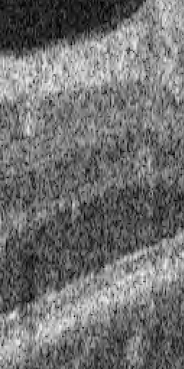
\includegraphics[width=0.18\linewidth]{figures/CirrusPatchExample.png}
	\caption{Example of a patch extracted from a Cirrus OCT volume used in Experiment 1.1. In this patch, while the background is noticeable due to its darker shade, the choroid is harder to be identified by an observer (or a model) due to the lack of context.}
	\label{fig:CirrusPatchExample}
\end{figure}

In Figure \ref{fig:Experiment11Segmentation}, it is shown a segmentation performed by the model trained in Run 1. In this figure it becomes evident that the model learned which areas can be segmented inside the retina, but does not understand how to handle the regions further away. For example, in the area significantly above the retina, the background is labeled as SRF. However, the background region closer to the retina is not so frequently labeled as any fluid, since it appears in the patches input to the model. The same problem occurs with the oversegmentation of PED in the choroid region, which does not appear in the input patches significantly. The fact that the patches are extracted exclusively from the ROI makes the model more prone to misclassify the background regions, as it did not see any patch that contained solely background.
\par
Oversegmentation beyond the retinal bounds is not exclusive to the Cirrus volumes, as it also appears in the OCT scans from other vendors. This suggests that the issue is primarily due to the small patch size and lack of background representitivity in the inputs rather than just the smaller retinal area captured in Cirrus patches, despite this amplifying the problem. 
\par
In the same figure, it is seen that the model has not learned the anatomical relationships between fluids, since it segmented IRF and PED close to each other. This occurs because the model has not learned the relationship between the retinal landmarks and the fluid types due to the small sized inputs.

\begin{figure}[!ht]
	\centering
	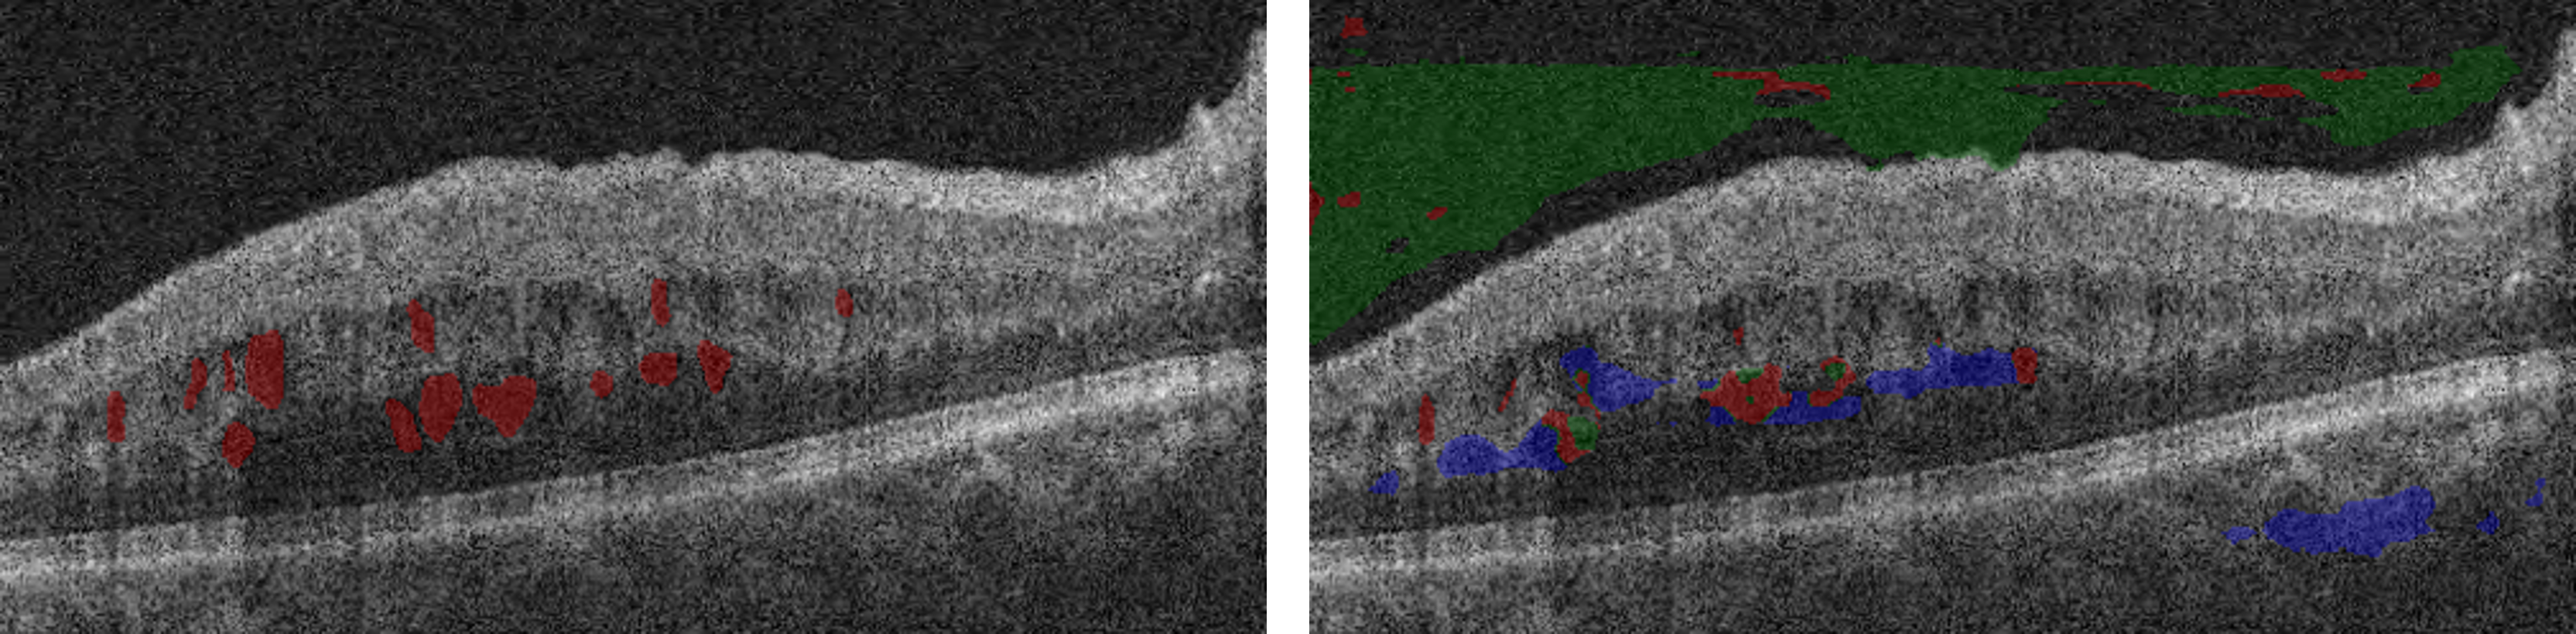
\includegraphics[width=1.0\linewidth]{figures/Experiment11Segmentation.png}
	\caption{Example of a poor segmentation made by the model trained in Run 1 (right). In the left, the GT mask for the same image is shown.}
	\label{fig:Experiment11Segmentation}
\end{figure}

\subsubsection{Experiment 1.2}

The resulting Dice coefficient values obtained in Experiment 1.2, where patches of shape 496 $\times$ 512 were used, are shown in Table \ref{tab:Experiment1.2Results}.

\begin{table*}[!ht]
	\caption{Dice scores for every vendor and fluid for the runs done in Experiment 1.2.}
	\centering
	\resizebox{\textwidth}{!}{\begin{tabular}{|c|c|ccc|ccc|ccc|c|c|c|c|}
		\hline
		% Headers
		\multirow{2}{*}{\textbf{Runs}} & 
		\multirow{2}{*}{\textbf{VF}} & 
		\multicolumn{3}{c|}{\textbf{Cirrus}} & 
		\multicolumn{3}{c|}{\textbf{Spectralis}} & 
		\multicolumn{3}{c|}{\textbf{Topcon}} & 
		\multicolumn{1}{c|}{\multirow{2}{*}{\textbf{IRF}}} & 
		\multirow{2}{*}{\textbf{SRF}} & 
		\multirow{2}{*}{\textbf{PED}} & 
		\multirow{2}{*}{\textbf{Fluid}} \\ \cline{3-11} & &
		\multicolumn{1}{c}{\textbf{IRF}} & 
		\multicolumn{1}{c}{\textbf{SRF}} & 
		\textbf{\textbf{PED}} & 
		\multicolumn{1}{c}{\textbf{IRF}} & 
		\multicolumn{1}{c}{\textbf{SRF}} & 
		\textbf{PED} & 
		\textbf{IRF} & 
		\textbf{SRF} & 
		\textbf{PED} & 
		\multicolumn{1}{c|}{} & & & \\ 
			
		\hline
		
		\textbf{Run 9} & 2 & \multicolumn{1}{c|}{0.291} & \multicolumn{1}{c|}{0.450} & 0.281 & \multicolumn{1}{c|}{0.472} & \multicolumn{1}{c|}{0.638} & 0.394 & \multicolumn{1}{c|}{0.505} & \multicolumn{1}{c|}{0.647} & 0.573 & 0.396 & 0.551 & 0.400 & 0.393 \\

		
		\textbf{Run 10} & 3 & \multicolumn{1}{c|}{\textbf{0.586}} & \multicolumn{1}{c|}{\textbf{0.619}} & \textbf{0.727} & \multicolumn{1}{c|}{0.482} & \multicolumn{1}{c|}{\textbf{0.780}} & \textbf{0.698} & \multicolumn{1}{c|}{\textbf{0.749}} & \multicolumn{1}{c|}{\textbf{0.793}} & \textbf{0.788} & \textbf{0.627} & \textbf{0.711} & \textbf{0.744} & \textbf{0.667} \\

		
		\textbf{Run 11} & 4 & \multicolumn{1}{c|}{0.281} & \multicolumn{1}{c|}{0.453} & 0.415 & \multicolumn{1}{c|}{0.429} & \multicolumn{1}{c|}{0.503} & 0.322 & \multicolumn{1}{c|}{0.228} & \multicolumn{1}{c|}{0.532} & 0.324 & 0.278 & 0.494 & 0.363 & 0.296 \\
		
		\textbf{Run 12} & 0 & \multicolumn{1}{c|}{0.242} & \multicolumn{1}{c|}{0.334} & 0.336 & \multicolumn{1}{c|}{\textbf{0.551}} & \multicolumn{1}{c|}{0.564} & 0.423 & \multicolumn{1}{c|}{0.321} & \multicolumn{1}{c|}{0.643} & 0.407 & 0.325 & 0.488 & 0.377 & 0.339 \\
		
		\hline
		
		\textbf{Set 3} & - & \multicolumn{1}{c|}{0.35} & \multicolumn{1}{c|}{0.46} & 0.44 & \multicolumn{1}{c|}{0.48} & \multicolumn{1}{c|}{0.62} & 0.46 & \multicolumn{1}{c|}{0.45} & \multicolumn{1}{c|}{0.65} & 0.52 & 0.41 & 0.56 & 0.47 & 0.42 \\
		
		\hline
		\hline
		
		\textbf{Set 2} & - & \multicolumn{1}{c|}{\textbf{0.35}} & \multicolumn{1}{c|}{\textbf{0.24}} & \textbf{0.32} & \multicolumn{1}{c|}{\textbf{0.34}} & \multicolumn{1}{c|}{\textbf{0.51}} & \textbf{0.47} & \multicolumn{1}{c|}{\textbf{0.43}} & \multicolumn{1}{c|}{\textbf{0.64}} & \textbf{0.36} & \textbf{0.38} & \textbf{0.44} & \textbf{0.36} & \textbf{0.27} \\ 
		
		\hline
					
	\end{tabular}}
	\label{tab:Experiment1.2Results}
\end{table*}

The information resumed in this table allows the comparison between the performance in models that used smaller patches in Experiment 1.1 with those that used larger patches in this Experiment.
\par
By comparing the ``Set'' rows, it becomes evident an overall increase in performance when using larger patches. In fact, it is observed an increase in almost all the mean values when compared to the best performing set in Experiment 1.1. This increase is larger than one decimal point in some columns, and the largest improvements occur in the volumes obtained using the Cirrus device and when segmenting SRF or PED.
\par
The improvement in performance in Cirrus devices can be explained with the more contextual information given. In Experiment 1.1, the Cirrus patches input to the model were not big enough for the network to capture and understand the retinal borders or the relationship between them and the fluids, and the networks were trained with the small representation of background, thus leading to oversegmentation beyond the retina, as explained. In Experiment 1.2, as the same patch covers the retinal layer and the background simultaneously, the model has learned to not segment beyond the retina. In Figure \ref{fig:BigPatchesSegmentationCirrus}, the B-scan shown in Figure \ref{fig:Experiment11Segmentation}, is segmented by the model trained in Run 9 and it is possible to see that the labeling of the background as fluid is no longer happening.
\par 
This also partially justifies the significant improvement in the SRF and PED Dice coefficient. By providing inputs with enough context, the model is no longer segmenting these fluids outside the retina. However, in Figure \ref{fig:BigPatchesSegmentationCirrus} it is also seen that the model is no longer confusing the fluids in the retina, as it no longer segments the PED close to the IRF. This further justifies that the model is learning the anatomical references associated with PED, as confirmed in Figure \ref{fig:BigPatchesSegmentationTopcon}.
\par
Lastly, it is important to note that the IRF did not improve as much as the other fluids. This happens because the input patches in Experiment 1.1 where extracted mainly from the retina, providing all the anatomical context needed for the IRF segmentation. By training the model with larger patches, its attention to the finer details is reduced, therefore not producing fine and detailed segmentations in smaller fluid regions.
\par
In Figure \ref{fig:BigPatchesSegmentationTopcon}, it is seen that the model confuses the choroid with the retina, as it labels parts of that region as IRF and PED. The likely cause for this confusion is that the input patches are often cropped in the middle of the retinal layer (as illustrated in Figure \ref{fig:BigPatchExtraction}), which leads to the model not understanding the position of the choroid relative to the retina. This inaccurate IRF and PED segmentation is probably based on the visual resemblance between the structures seen in the choroid and the fluid regions in the retina. This indicates that the model does not know the location of the choroid.

\begin{figure}[!ht]
	\centering
	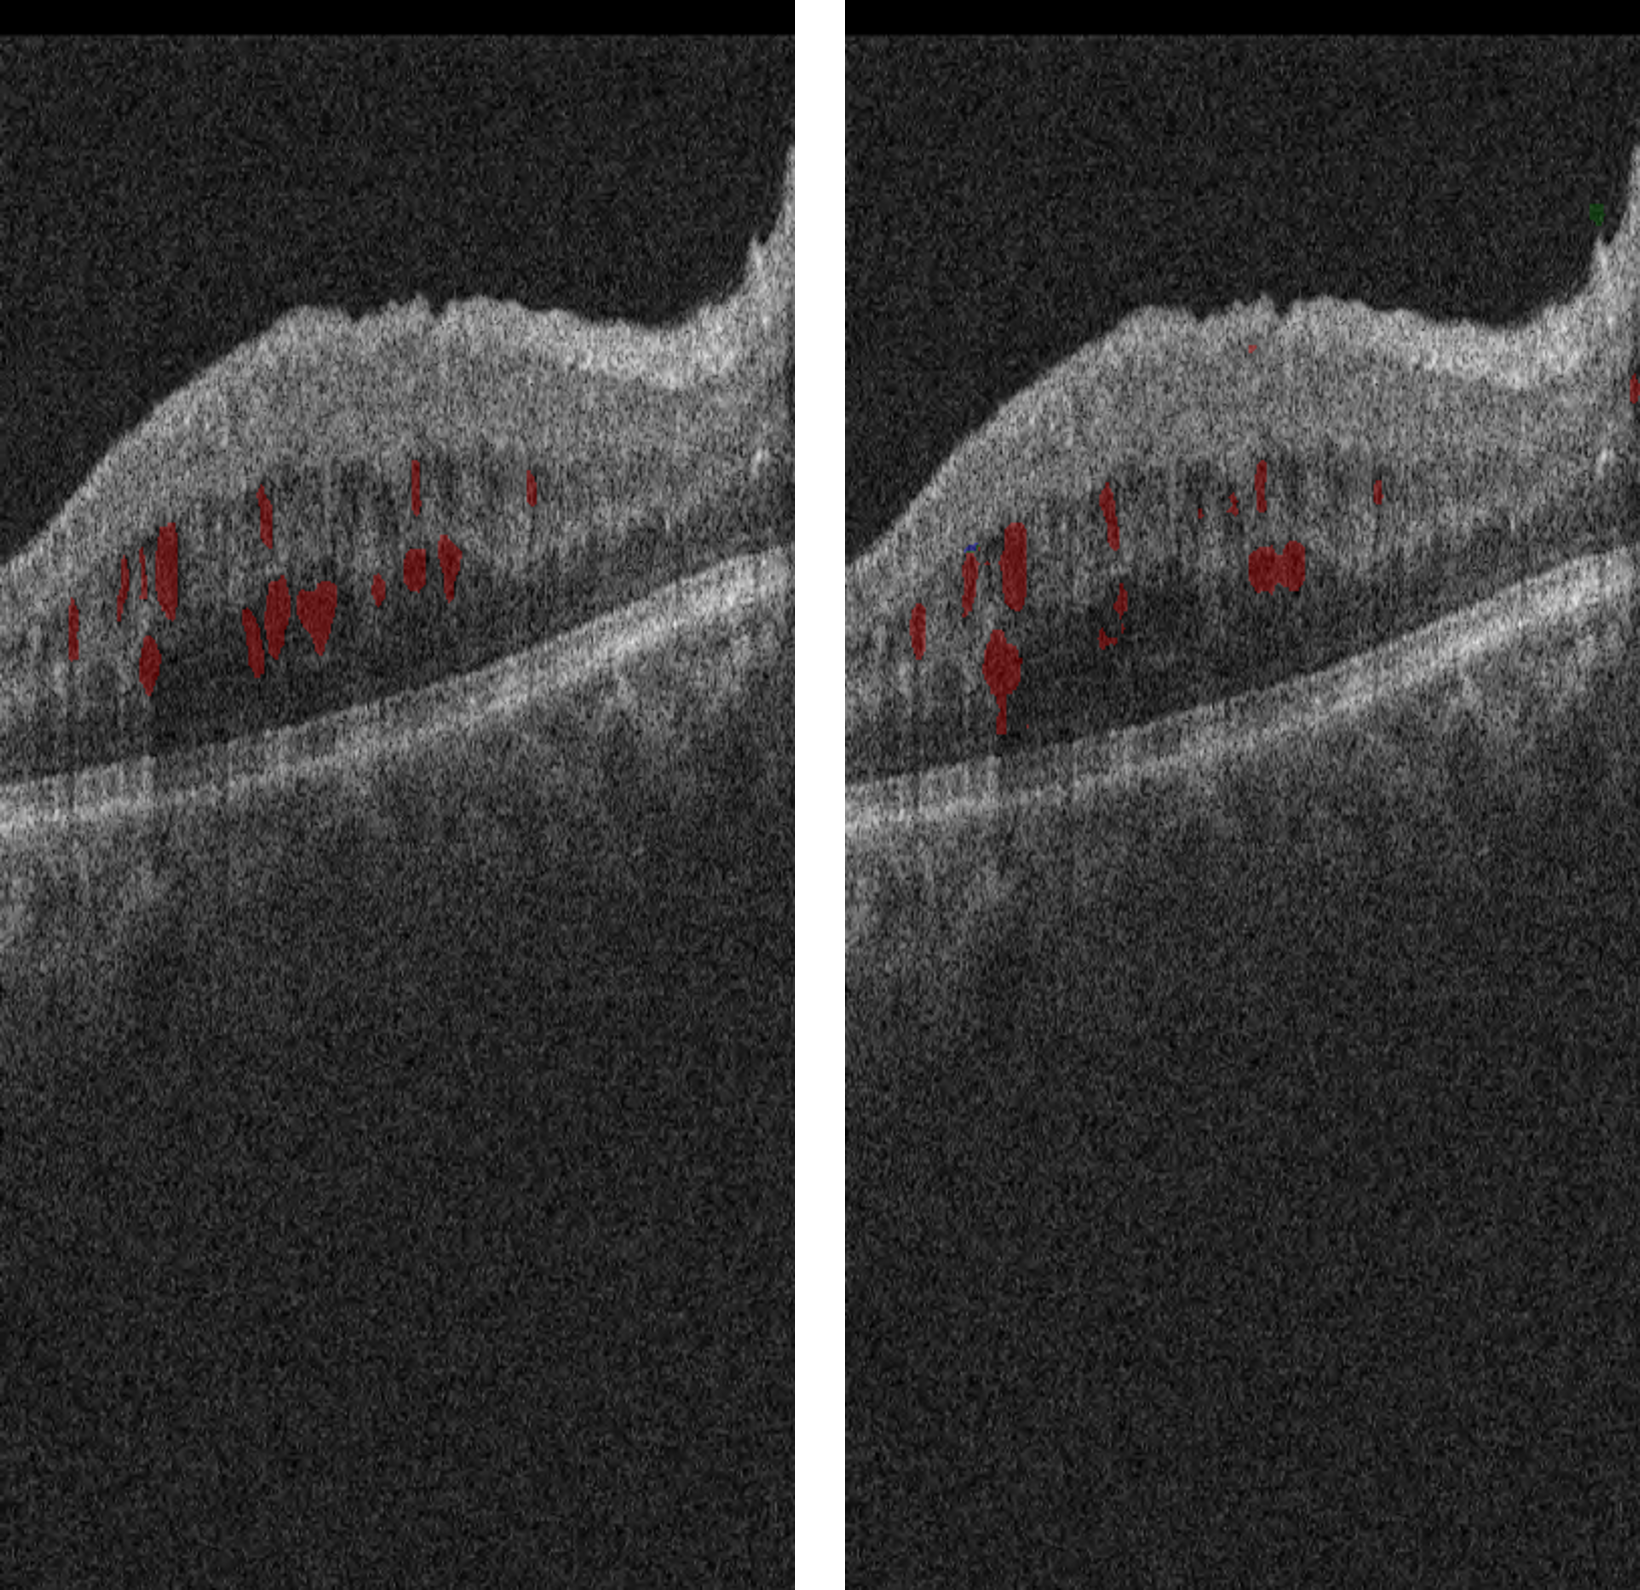
\includegraphics[width=0.5\linewidth]{figures/BigPatchSegmentationCirrus.png}
	\caption{Example of the segmentation done by the model trained in Run 9 (right) and its respective GT mask (left). The B-scan segmented is the same as in Figure \ref{fig:Experiment11Segmentation}.}
	\label{fig:BigPatchesSegmentationCirrus}
\end{figure}

\begin{figure}[!ht]
	\centering
	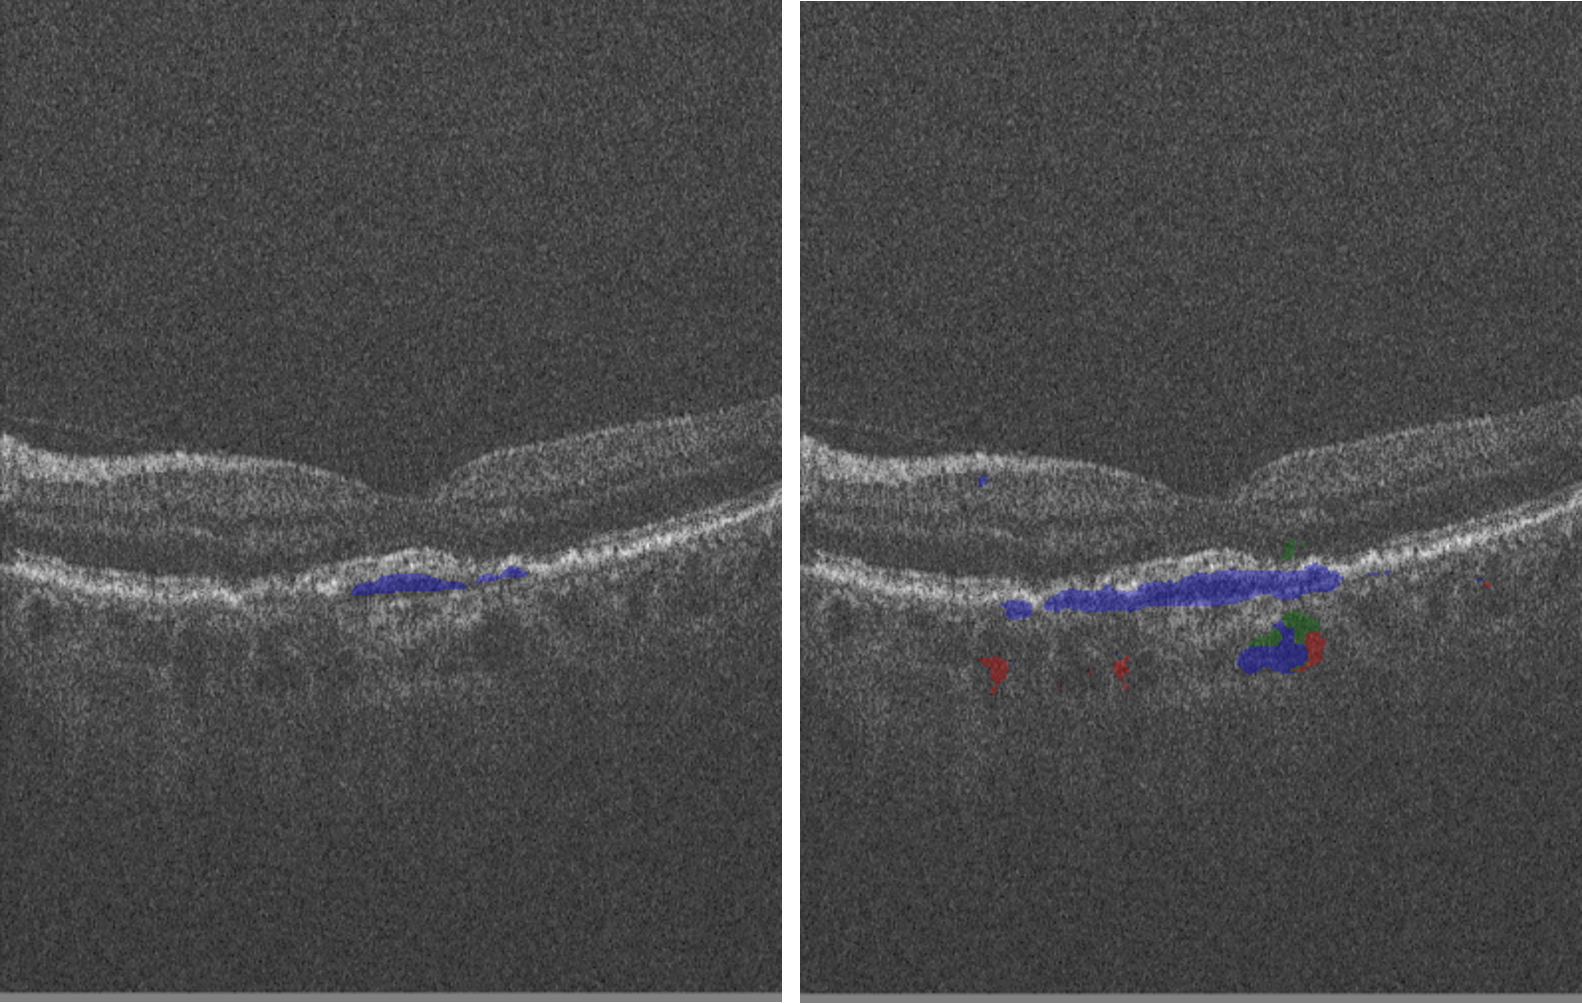
\includegraphics[width=0.6\linewidth]{figures/BigPatchSegmentationTopcon.png}
	\caption{Example of the segmentation done by the model trained in Run 12 (right) and its respective GT mask (left). It is noticeable that the model confuses the choroid with the retina, as segmentation of IRF and PED is performed in the choroid.}
	\label{fig:BigPatchesSegmentationTopcon}
\end{figure}

\subsubsection{Experiment 1.3}
Experiment 1.3 contains all the runs that were performed using vertical patches extracted from resized B-scans as input of the multi-class segmentation U-Net. In the first two sets, shown in Table \ref{tab:Experiment1.3FourPatches}, the models were trained using four vertical patches, obtained as explained in the \ref{Methods} Methods chapter. In this table, the ``Set 4'' is composed of runs that were trained on 100 epochs, while the runs in ``Set 5'' were trained on up to 200 epochs with a 100 epoch patience.

\begin{table*}[!ht]
	\caption{Dice scores for every vendor and fluid for the runs done using four vertical patches extracted from each B-scan. In ``Set 4'', the models were trained in 100 epochs, while in ``Set 5'' the models were trained on up to 200 epochs with a 100 epoch patience. The transformations applied in these sets were the same: horizontal flipping and a maximum rotation of $10^{\circ}$.}
	\centering
	\resizebox{\textwidth}{!}{\begin{tabular}{|c|c|ccc|ccc|ccc|c|c|c|c|}
		\hline
		% Headers
		\multirow{2}{*}{\textbf{Runs}} & 
		\multirow{2}{*}{\textbf{VF}} & 
		\multicolumn{3}{c|}{\textbf{Cirrus}} & 
		\multicolumn{3}{c|}{\textbf{Spectralis}} & 
		\multicolumn{3}{c|}{\textbf{Topcon}} & 
		\multicolumn{1}{c|}{\multirow{2}{*}{\textbf{IRF}}} & 
		\multirow{2}{*}{\textbf{SRF}} & 
		\multirow{2}{*}{\textbf{PED}} & 
		\multirow{2}{*}{\textbf{Fluid}} \\ \cline{3-11} & &
		\multicolumn{1}{c}{\textbf{IRF}} & 
		\multicolumn{1}{c}{\textbf{SRF}} & 
		\textbf{\textbf{PED}} & 
		\multicolumn{1}{c}{\textbf{IRF}} & 
		\multicolumn{1}{c}{\textbf{SRF}} & 
		\textbf{PED} & 
		\textbf{IRF} & 
		\textbf{SRF} & 
		\textbf{PED} & 
		\multicolumn{1}{c|}{} & & & \\ 
			
		\hline
		
		\textbf{Run 13} & 2 & \multicolumn{1}{c|}{0.411} & \multicolumn{1}{c|}{0.665} & 0.498 & \multicolumn{1}{c|}{0.654} & \multicolumn{1}{c|}{0.735} & 0.611 & \multicolumn{1}{c|}{0.731} & \multicolumn{1}{c|}{0.743} & 0.519 & 0.563 & 0.704 & 0.526 & 0.581 \\

		\textbf{Run 14} & 3 & \multicolumn{1}{c|}{0.390} & \multicolumn{1}{c|}{0.520} & 0.217 & \multicolumn{1}{c|}{0.403} & \multicolumn{1}{c|}{0.564} & 0.429 & \multicolumn{1}{c|}{0.378} & \multicolumn{1}{c|}{0.754} & 0.477 & 0.388 & 0.614 & 0.350 & 0.386 \\
		
		\textbf{Run 15} & 4 & \multicolumn{1}{c|}{0.792} & \multicolumn{1}{c|}{\textbf{0.846}} & \textbf{0.883} & \multicolumn{1}{c|}{0.732} & \multicolumn{1}{c|}{\textbf{0.901}} & 0.733 & \multicolumn{1}{c|}{0.615} & \multicolumn{1}{c|}{0.758} & 0.656 & 0.707 & 0.815 & 0.765 & 0.652 \\
		
		\textbf{Run 16} & 0 & \multicolumn{1}{c|}{\textbf{0.810}} & \multicolumn{1}{c|}{0.834} & 0.715 & \multicolumn{1}{c|}{0.779} & \multicolumn{1}{c|}{0.857} & 0.753 & \multicolumn{1}{c|}{0.783} & \multicolumn{1}{c|}{\textbf{0.924}} & \textbf{0.882} & \textbf{0.795} & \textbf{0.871} & \textbf{0.783} & \textbf{0.709} \\
		
		\hline
		
		\textbf{Set 4} & - & \multicolumn{1}{c|}{\textbf{0.60}} & \multicolumn{1}{c|}{\textbf{0.72}} & 0.58 & \multicolumn{1}{c|}{0.64} & \multicolumn{1}{c|}{\textbf{0.76}} & 0.63 & \multicolumn{1}{c|}{0.63} & \multicolumn{1}{c|}{\textbf{0.79}} & 0.63 & 0.61 & \textbf{0.75} & 0.61 & 0.58 \\
		
		\hline
		\hline
		
		\textbf{Run 17} & 2 & \multicolumn{1}{c|}{0.522} & \multicolumn{1}{c|}{0.784} & 0.703 & \multicolumn{1}{c|}{\textbf{0.805}} & \multicolumn{1}{c|}{0.765} & \textbf{0.865} & \multicolumn{1}{c|}{\textbf{0.828}} & \multicolumn{1}{c|}{0.879} & 0.835 & 0.677 & 0.813 & 0.777 & 0.684 \\
	
		\textbf{Run 18} & 3 & \multicolumn{1}{c|}{0.509} & \multicolumn{1}{c|}{0.654} & 0.598 & \multicolumn{1}{c|}{0.590} & \multicolumn{1}{c|}{0.806} & 0.755 & \multicolumn{1}{c|}{0.777} & \multicolumn{1}{c|}{0.787} & 0.792 & 0.621 & 0.729 & 0.697 & 0.622 \\
					
		\textbf{Run 19} & 4 & \multicolumn{1}{c|}{0.377} & \multicolumn{1}{c|}{0.387} & 0.398 & \multicolumn{1}{c|}{0.478} & \multicolumn{1}{c|}{0.624} & 0.398 & \multicolumn{1}{c|}{0.483} & \multicolumn{1}{c|}{0.729} & 0.448 & 0.436 & 0.567 & 0.420 & 0.399 \\
		
		\textbf{Run 20} & 0 & \multicolumn{1}{c|}{0.753} & \multicolumn{1}{c|}{0.697} & 0.696 & \multicolumn{1}{c|}{0.779} & \multicolumn{1}{c|}{0.844} & 0.783 & \multicolumn{1}{c|}{0.691} & \multicolumn{1}{c|}{0.720} & 0.671 & 0.735 & 0.731 & 0.702 & 0.637 \\
		
		\hline
		
		\textbf{Set 5} & - & \multicolumn{1}{c|}{0.54} & \multicolumn{1}{c|}{0.63} & \textbf{0.60} & \multicolumn{1}{c|}{\textbf{0.66}} & \multicolumn{1}{c|}{0.76} & \textbf{0.70} & \multicolumn{1}{c|}{\textbf{0.69}} & \multicolumn{1}{c|}{0.78} & \textbf{0.69} & \textbf{0.62} & 0.71 & \textbf{0.65} & \textbf{0.59} \\
		
		\hline
			
	\end{tabular}}
	\label{tab:Experiment1.3FourPatches}
\end{table*}

The results of the sets shown in Table \ref{tab:Experiment1.3FourPatches} can be compared within each other and to the results obtained in the sets of previous experiments. 
\par
When comparing the results between sets, it is noticeable that the runs with the best scores are mostly located in the ``Set'' that trained less epochs. For, the model validated on fold 4 (Run 15) sees a significant decrease in performance when trained for 100 more epochs (Run 19). When looking at the models validation loss per epoch, the lowest value is attained commonly before the 100 epochs. Since the model that is saved in each run is the model that attains the lowest loss on validation data, this means that the models trained in 100 or 200 epochs should perform equally, as long as the lowest validation loss occurred prior to the 100 epoch mark.
\par
However, looking at Figure \ref{fig:TrainingValidationLosses}, where the training and validation loss curves for the Run 13 and Run 17 are shown, similar trends and behavior is seen in both models. This does not reflect to similar performances in the same validation data, as shown in Table \ref{tab:Experiment1.3FourPatches}. In fact, a substantial increment is seen in Run 17.
\par
To justify this behavior, it is important to remind that the training of a neural network has some randomness associated with it. One aspect that affects the model performance despite using the same data and architecture is the weight initialization. The random initialization of weights affects the trajectory of gradient descent, resulting in different convergences for different runs. Another factor that affects the model learning is the data that composes each batch. The images that form a batch are randomly fetch from the available input images. This create batches with different distributions of characteristics, affecting the model's view of the data. Data augmentation, which randomly selects images to apply the transformations as they are fetch, also influences the model performance. Lastly, there are other factors that have a much smaller impact such as the optimizer behavior and non-deterministic operations at the GPU level \parencite{Akesson2024, Altarabichi2024}. 
\par
In Appendix \ref{ap1:SegmentationUNetVariability}, Table \ref{tab:SegmentationUNetVariability} shows the results for multiple models that were trained on the same conditions, aiming to give an insight on how the randomness associated with the U-Net affects the models performances. Five models were validated on fold 2, while nine models were validated in fold 3. The results obtained corroborate the differences seen in Table \ref{tab:Experiment1.3FourPatches}, where models trained on the same conditions for more epochs can obtain significantly worse Dice scores in validation.

\begin{figure}[!ht]
	\centering
	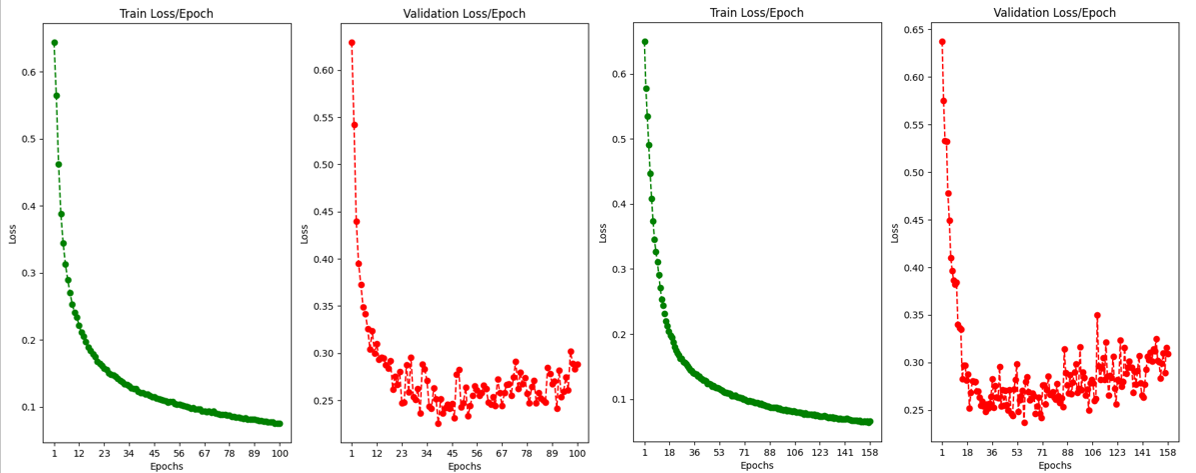
\includegraphics[width=1.0\linewidth]{figures/TrainingValidationLosses.png}
	\caption{Training and validation losses in Run 13 (left) and Run 17 (right). Despite reaching the validation loss minimum in a similar number of epochs and having comparable training and validation loss curves, the performance is really different in Table \ref{tab:Experiment1.3FourPatches}.}
	\label{fig:TrainingValidationLosses}
\end{figure}

Despite the differences in the results shown in Table \ref{tab:Experiment1.3FourPatches}, both sets attained better performances than the best results in the previous experiments. The improvements were significant, registering increases above 0.2 in some metrics when compared with the results in Experiment 1.3. Every vendor and every fluid seen a considerable increase of performance.
\par
This overall increment can be attributed to two changes: training on vertical patches and resizing the images. By training the models on vertical patches, the model can focus on the finer details within each region. This is important because the retinal fluid segmentation relies heavily on the retina's characteristics, a region that occupies a small portion of the image. Despite the input being smaller than in Experiment 1.2, the patches could still capture the transitions between the retina and the choroid or background. Since the input size is smaller, less storage it occupies in memory, therefore allowing an increase in the batch size, that translates to a faster and more stable convergence. Meanwhile, the image's resizing makes the inputs more homogeneous across different vendors. This results in the same structures being represented with consistent shapes and sizes across the B-scans from different vendors, resulting in a significantly simpler learning process.
\par
It was seen in Figure \ref{fig:BigPatchesSegmentationTopcon} that the model predicted fluid masks in the choroid region. In Figure \ref{fig:VerticalPatchesSegmentationTopcon}, it is seen that the models trained on vertical patches no longer predict fluid in the choroid region, despite inferring on the same B-scan. This means that, by feeding vertical patches to the model, it learns to not segment below the retina, in the choroid. This was not previously understood by the model when big patches were input, since these would frequently not capture both the retinal layer and the choroid in the same patch, restraining the model from learning the relative position of the choroid and its relationship with the fluid prediction.

\begin{figure}[!ht]
	\centering
	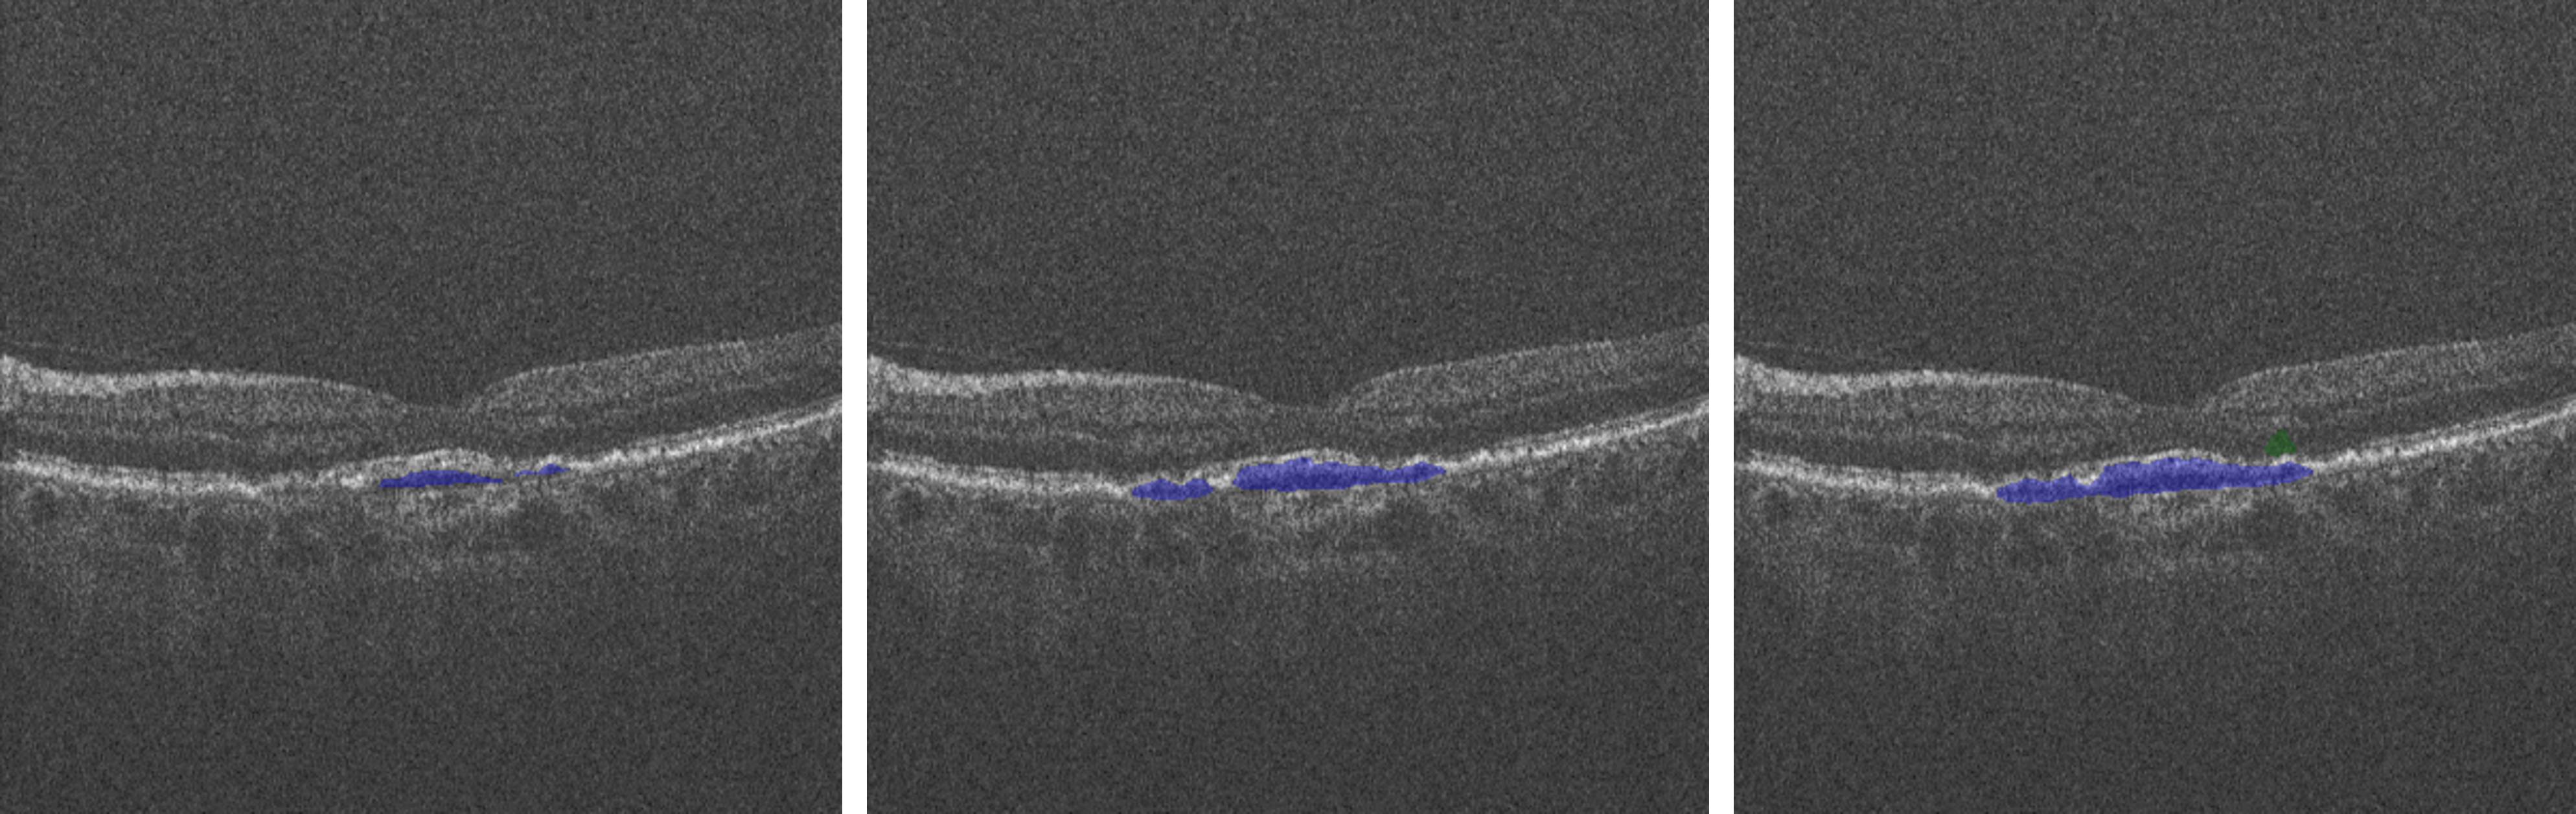
\includegraphics[width=1.0\linewidth]{figures/VerticalPatchesSegmentationTopcon.png}
	\caption{Predicted masks by the models trained on Run 16 (middle) and Run 20 (right) and their respective GT (left).}
	\label{fig:VerticalPatchesSegmentationTopcon}
\end{figure}

Afterwards, the use of seven and thirteen patches extracted from each B-scan was tested and the results are shown in Table \ref{tab:Experiment1.3SevenVsThirteenPatches}. Two models were trained for each number of patches extracted, one validated on fold 2 and another validated on fold 3. The models were trained on 200 maximum epochs, with a 25 epoch patience applied after the first 100 epochs.

\begin{table*}[!ht]
	\caption{Dice scores for every vendor and fluid for the runs done using seven (Runs 21 and 22) and thirteen (Runs 23 and 24) vertical patches extracted from each B-scan. Only two folds were used in order to understand the viability of using these numbers of patches, which are represented in the column ``P''. Runs 17 and 18 are shown here to make the comparison between the number of patches easier. The values shown in bold represent the best value for the models validated in the same fold.}
	\centering
	\resizebox{\textwidth}{!}{\begin{tabular}{|c|c|c|ccc|ccc|ccc|c|c|c|c|}
		\hline
		% Headers
		\multirow{2}{*}{\textbf{Runs}} & 
		\multirow{2}{*}{\textbf{VF}} & 
		\multirow{2}{*}{\textbf{P}} &
		\multicolumn{3}{c|}{\textbf{Cirrus}} & 
		\multicolumn{3}{c|}{\textbf{Spectralis}} & 
		\multicolumn{3}{c|}{\textbf{Topcon}} & 
		\multicolumn{1}{c|}{\multirow{2}{*}{\textbf{IRF}}} & 
		\multirow{2}{*}{\textbf{SRF}} & 
		\multirow{2}{*}{\textbf{PED}} & 
		\multirow{2}{*}{\textbf{Fluid}} \\ \cline{4-12} & & &
		\multicolumn{1}{c}{\textbf{IRF}} & 
		\multicolumn{1}{c}{\textbf{SRF}} & 
		\textbf{\textbf{PED}} & 
		\multicolumn{1}{c}{\textbf{IRF}} & 
		\multicolumn{1}{c}{\textbf{SRF}} & 
		\textbf{PED} & 
		\textbf{IRF} & 
		\textbf{SRF} & 
		\textbf{PED} & 
		\multicolumn{1}{c|}{} & & & \\ 
		
		\hline
			
		\textbf{Run 17} & 2 & 4 & \multicolumn{1}{c|}{0.522} & \multicolumn{1}{c|}{0.784} & \textbf{0.703} & \multicolumn{1}{c|}{\textbf{0.805}} & \multicolumn{1}{c|}{0.765} & \textbf{0.865} & \multicolumn{1}{c|}{0.828} & \multicolumn{1}{c|}{0.879} & 0.835 & 0.677 & 0.813 & \textbf{0.777} & 0.684 \\
		
		\textbf{Run 21} & 2 & 7 & \multicolumn{1}{c|}{\textbf{0.556}} & \multicolumn{1}{c|}{\textbf{0.837}} & 0.672 & \multicolumn{1}{c|}{0.761} & \multicolumn{1}{c|}{\textbf{0.853}} & 0.848 & \multicolumn{1}{c|}{\textbf{0.829}} & \multicolumn{1}{c|}{0.908} & \textbf{0.858} & \textbf{0.685} & \textbf{0.864} & 0.767 & \textbf{0.681} \\
		
		\textbf{Run 23} & 2 & 13 & \multicolumn{1}{c|}{0.500} & \multicolumn{1}{c|}{0.762} & 0.635 & \multicolumn{1}{c|}{0.672} & \multicolumn{1}{c|}{0.790} & 0.773 & \multicolumn{1}{c|}{0.819} & \multicolumn{1}{c|}{\textbf{0.936}} & 0.805 & 0.639 & 0.826 & 0.718 & 0.637 \\
		
		\hline
		\hline
		
		\textbf{Run 18} & 3 & 4 & \multicolumn{1}{c|}{0.509} & \multicolumn{1}{c|}{0.654} & 0.598 & \multicolumn{1}{c|}{0.590} & \multicolumn{1}{c|}{0.806} & \textbf{0.755} & \multicolumn{1}{c|}{\textbf{0.777}} & \multicolumn{1}{c|}{\textbf{0.787}} & \textbf{0.792} & 0.621 & 0.729 & 0.697 & 0.622 \\
		
		\textbf{Run 22} & 3 & 7 & \multicolumn{1}{c|}{\textbf{0.734}} & \multicolumn{1}{c|}{\textbf{0.855}} & 0.836 & \multicolumn{1}{c|}{\textbf{0.636}} & \multicolumn{1}{c|}{\textbf{0.846}} & 0.689 & \multicolumn{1}{c|}{0.686} & \multicolumn{1}{c|}{0.781} & 0.731 & \textbf{0.700} & \textbf{0.822} & \textbf{0.771} & \textbf{0.672} \\
		
		\textbf{Run 24} & 3 & 13 & \multicolumn{1}{c|}{0.612} & \multicolumn{1}{c|}{0.648} & \textbf{0.882} & \multicolumn{1}{c|}{0.455} & \multicolumn{1}{c|}{0.636} & 0.548 & \multicolumn{1}{c|}{0.499} & \multicolumn{1}{c|}{0.593} & 0.668 & 0.542 & 0.622 & 0.745 & 0.536 \\
		
		\hline
			
	\end{tabular}}
	\label{tab:Experiment1.3SevenVsThirteenPatches}
\end{table*}

Training the models on more patches per B-scan, significantly increases the quantity of data that is seen by the model during an epoch. Therefore, each epoch takes much longer to complete, requiring more computation power, leading to often bottlenecks. However, since the model sees many more patches per epoch, the model reaches the validation loss minimum much earlier than in the models trained with four patches. 
\par
In Figure \ref{fig:ValidationLossesFourSevenThirteenPatches}, it is possible to see a comparison between the training and validation losses of the models validated on fold 2, using four, seven, and thirteen vertical patches per B-scan. Despite following the same trends, the model learns significantly faster as the number of patches increases, resulting in a faster progression of the validation loss. As a result the models starts to overfit much earlier and aggressively with larger number of patches, which is signaled by the increase in validation loss after reaching low values.

\begin{figure}[!ht]
	\centering
	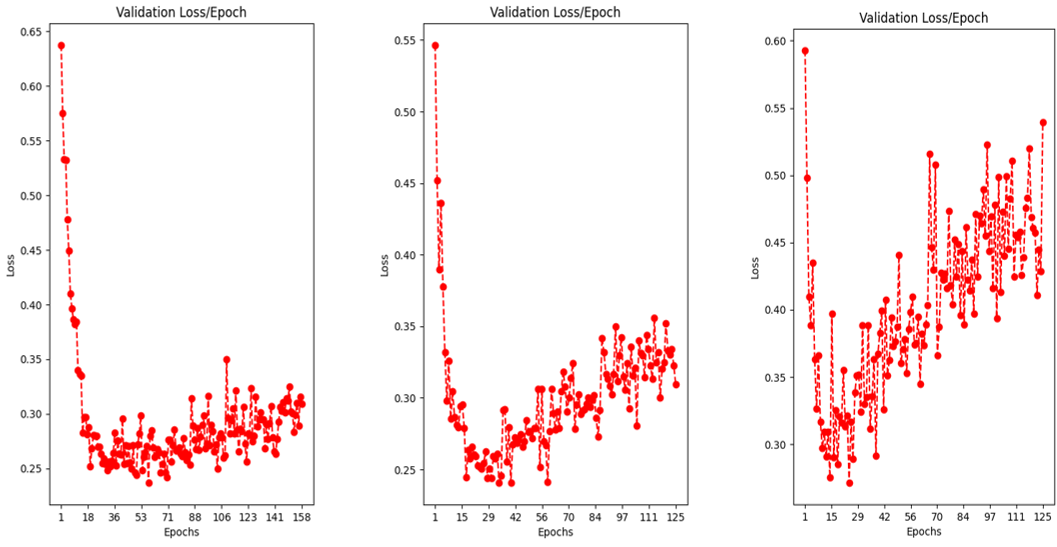
\includegraphics[width=1.0\linewidth]{figures/ValidationLossesFourSevenThirteenPatches.png}
	\caption{Training and validation losses for models validated on fold 2. The curve on the left are from the model trained on Run 17 with four patches, while the middle curves are from the model trained on Run 21, with seven patches. The curves on the right are from the model trained on Run 23, with thirteen patches.}
	\label{fig:ValidationLossesFourSevenThirteenPatches}
\end{figure}

When comparing the models' performances, by looking at Table \ref{tab:Experiment1.3FourPatches}, the models trained on thirteen patches are outperformed by those trained in fewer patches. These results suggest that the faster progression in validation loss for the model trained with thirteen patches inhibits its ability to converge to a solution as optimal as those achieved by models trained more slowly with fewer patches.
\par
The performance differences between the models trained with four and seven patches are smaller than the difference between either of those models and the model trained with thirteen patches. However, the model trained with seven patches consistently outperforms the one trained with four in most metrics. In the few cases the model trained with four patches performs better, the other model still achieves comparable results. The reverse is not true: when the model trained with seven patches outperforms the model trained with four patches, the performance gap is significantly larger. For these reasons, the model trained with seven patches was considered superior.
\par
Nevertheless, both models still make wrongful predictions, which do not respect the anatomic context of the image. For example, in Figure \ref{fig:CirrusSegmentationErrors}, the IRF fluid is predicted below the PED, which is not anatomically possible and there are no examples in the dataset that exhibit this relationship.
\par
While this unexpected behavior could be attributed to the B-scan differing from the examples seen in training, the subsequent runs aimed to investigate whether this was caused by the rotation transformation. It was hypothesized that random rotations could alter the vertical order of fluid regions, potentially leading the model to learn incorrect patterns. Additionally, the padding that is performed to fill the rotated areas, as illustrated in Figure \ref{fig:TransformationsInVerticalPatches}, could also influence the model's performance.

\begin{figure}[!ht]
	\centering
	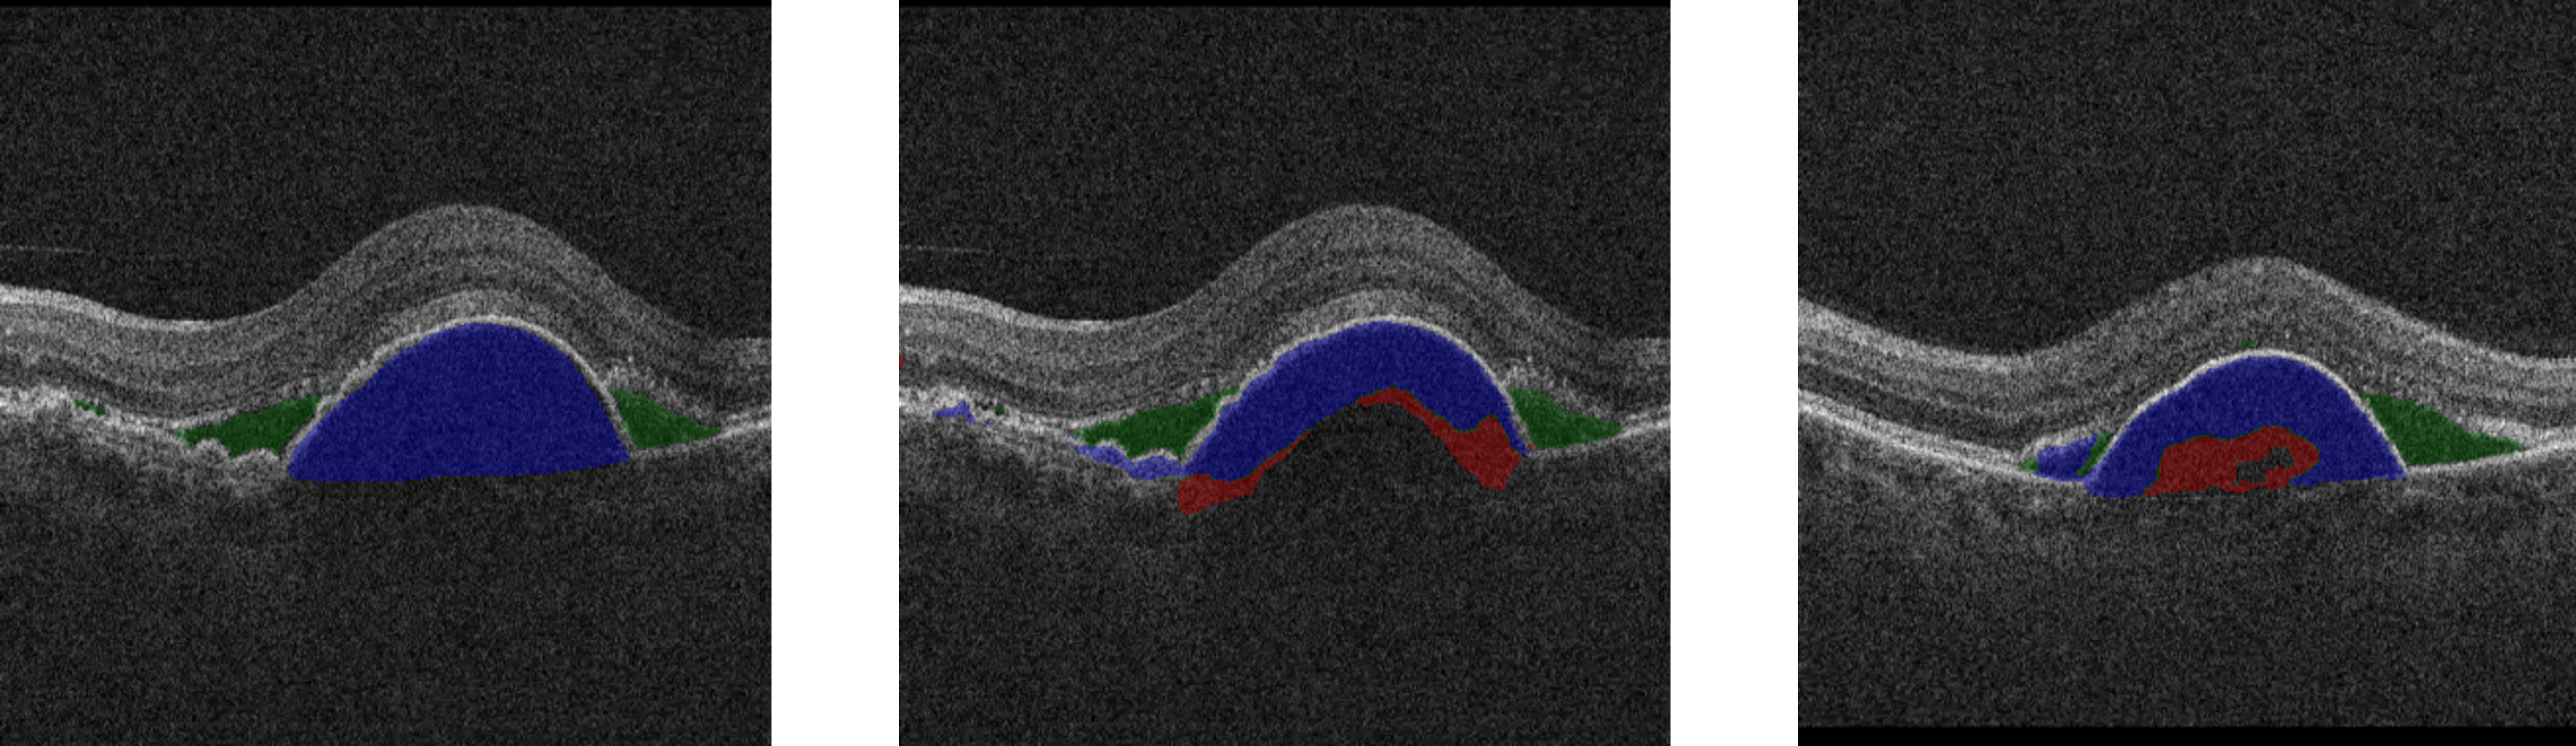
\includegraphics[width=1.0\linewidth]{figures/CirrusSegmentationErrors.png}
	\caption{Segmentation errors in Cirrus B-scans. The GT fluid masks, seen on the left, show a large region of PED fluid. Meanwhile, the predictions made by the models trained in Run 21 and 23, which respectively correspond to the B-scans in the middle and right, classify the center of this region as IRF.}
	\label{fig:CirrusSegmentationErrors}
\end{figure}

\begin{figure}[!ht]
	\centering
	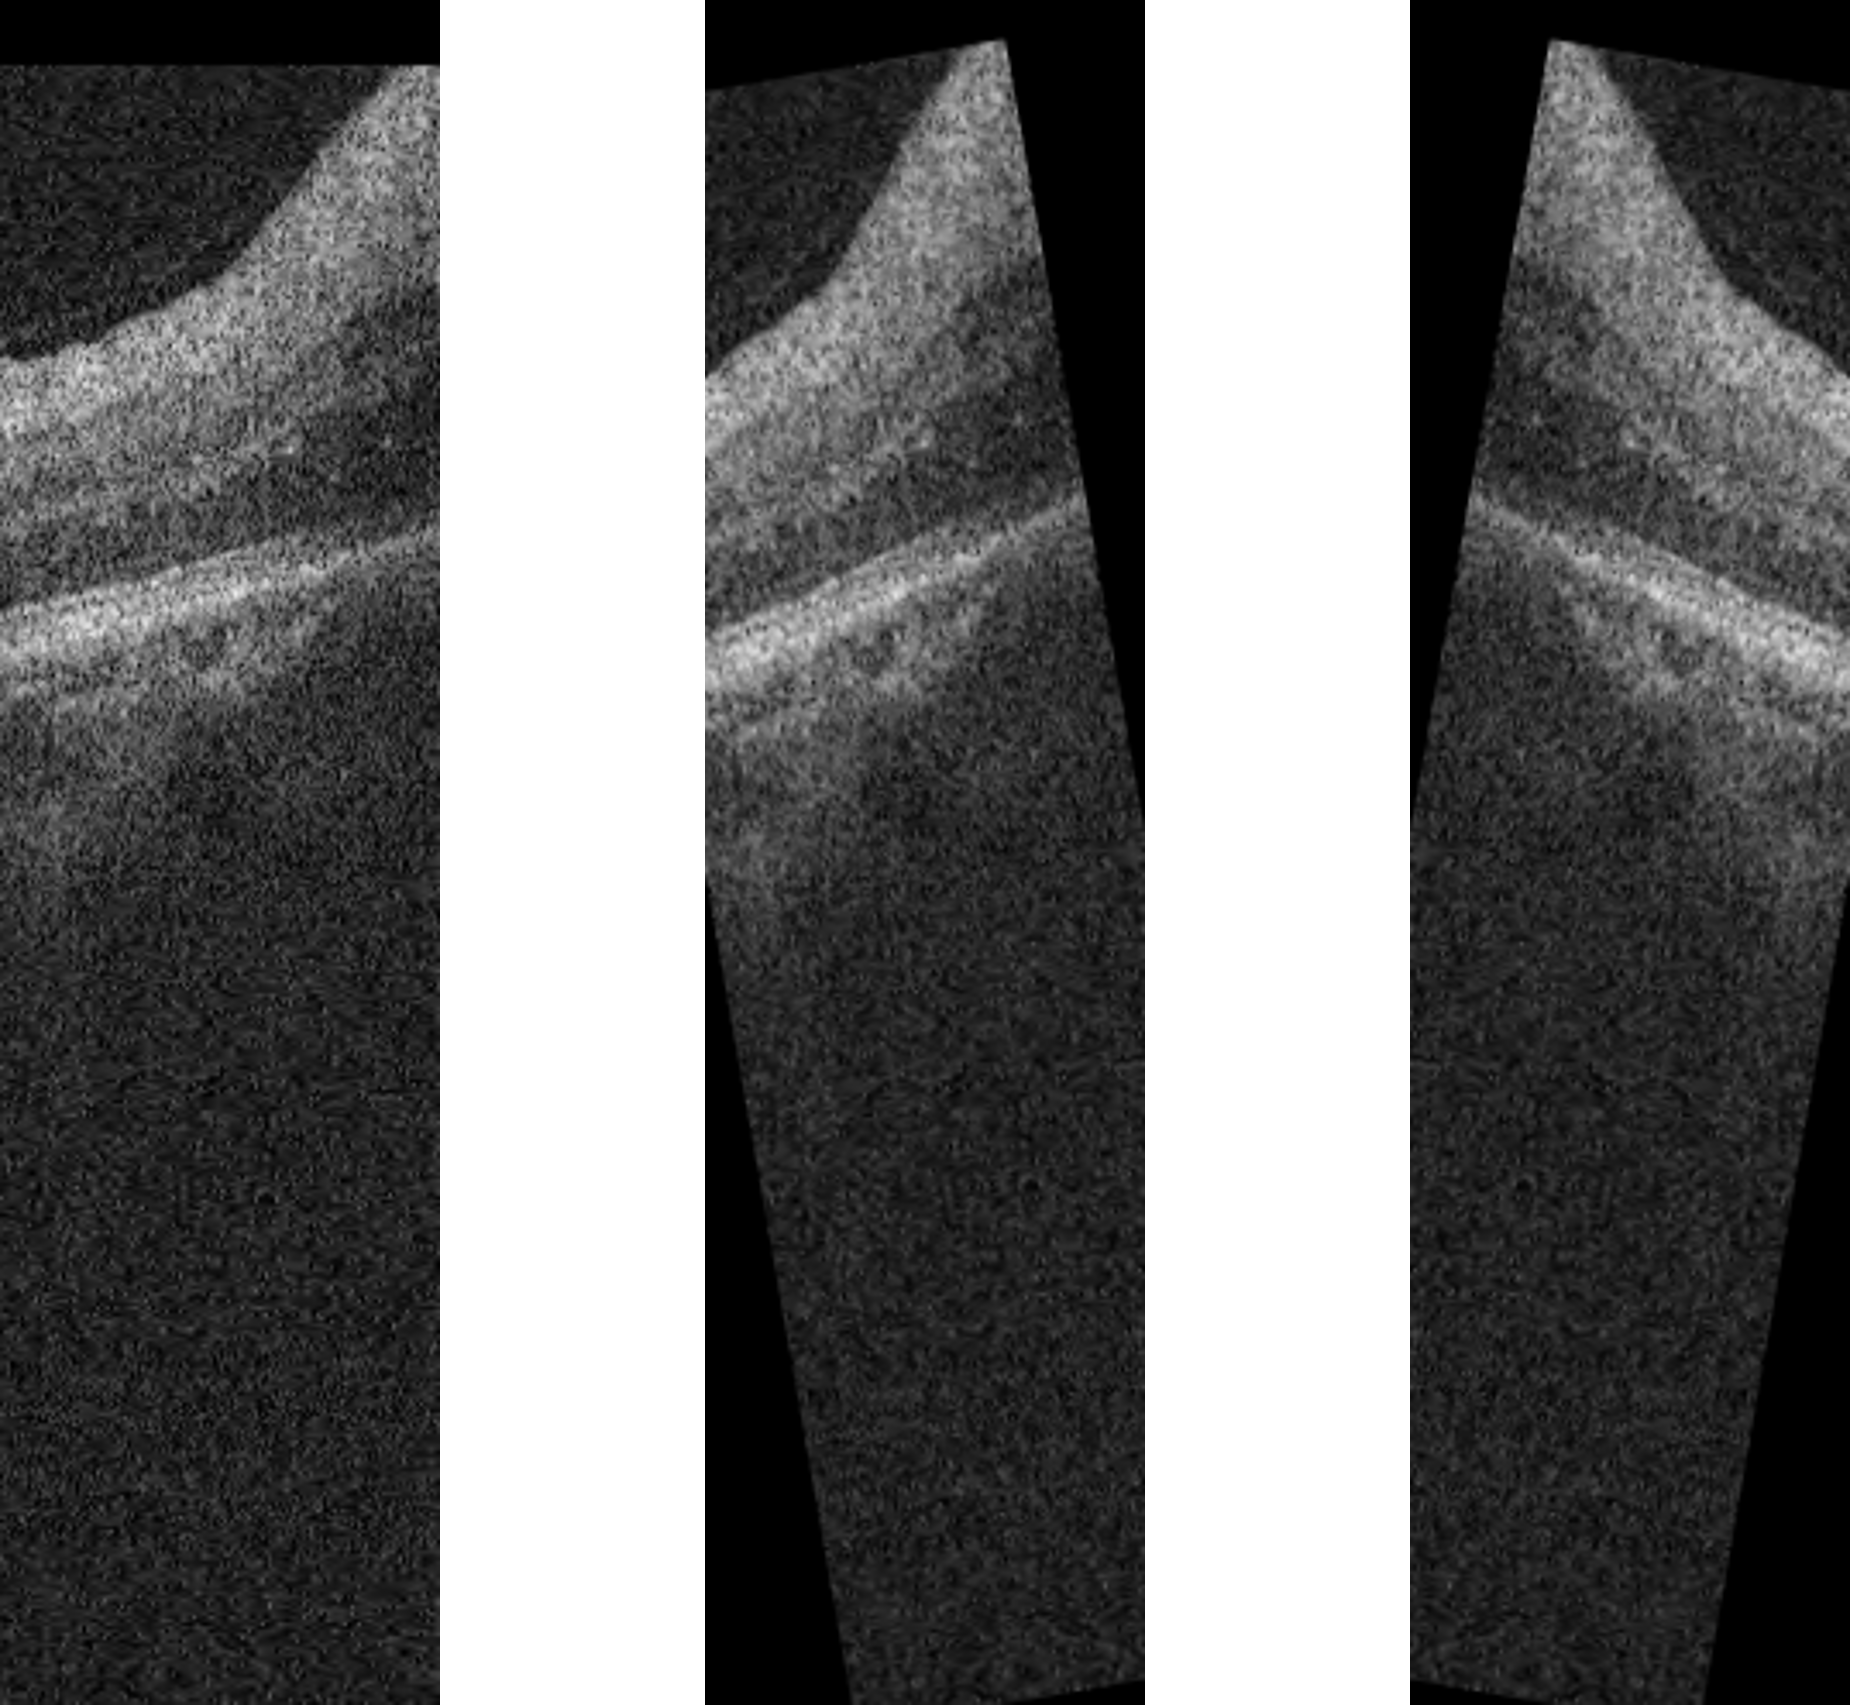
\includegraphics[width=0.5\linewidth]{figures/TransformationsInVerticalPatches.png}
	\caption{Transformations applied to a vertical patch of a Cirrus B-scan. The original vertical patch (left) can be rotated a maximum of $10^{\circ}$, a transformation that is shown in the middle image. The image on the right represents the combination of a $10^{\circ}$ rotation and an horizontal flip. It is seen that the rotation transform pads a significant portion of the image, reducing the information in the input.}
	\label{fig:TransformationsInVerticalPatches}
\end{figure}

Table \ref{tab:Experiment1.3SevenPatchesNoRotation} shows the results obtained in the runs performed using only horizontal flipping as transformation, without performing rotations. In these runs, seven input patches were extracted from each B-scan. Due to the faster progression of the models trained using seven vertical patches per B-scan, the model was trained on a minimum of 25 epochs with a 25 epoch patience after. Since the validation minimum is usually attained early in the models trained with more patches, as seen in Figure \ref{fig:ValidationLossesFourSevenThirteenPatches}, by setting such early stopping, the training duration would be shorter while maintaining the same performance.

\begin{table*}[!ht]
	\caption{Dice scores for every vendor and fluid using seven vertical patches. The only transformation performed in these runs was horizontal flipping, without rotation. Runs 21 and 22 are also shown, promoting an easier comparison.}
	\centering
	\resizebox{\textwidth}{!}{\begin{tabular}{|c|c|ccc|ccc|ccc|c|c|c|c|}
			\hline
			% Headers
			\multirow{2}{*}{\textbf{Runs}} & 
			\multirow{2}{*}{\textbf{VF}} & 
			\multicolumn{3}{c|}{\textbf{Cirrus}} & 
			\multicolumn{3}{c|}{\textbf{Spectralis}} & 
			\multicolumn{3}{c|}{\textbf{Topcon}} & 
			\multicolumn{1}{c|}{\multirow{2}{*}{\textbf{IRF}}} & 
			\multirow{2}{*}{\textbf{SRF}} & 
			\multirow{2}{*}{\textbf{PED}} & 
			\multirow{2}{*}{\textbf{Fluid}} \\ \cline{3-11} & &
			\multicolumn{1}{c}{\textbf{IRF}} & 
			\multicolumn{1}{c}{\textbf{SRF}} & 
			\textbf{\textbf{PED}} & 
			\multicolumn{1}{c}{\textbf{IRF}} & 
			\multicolumn{1}{c}{\textbf{SRF}} & 
			\textbf{PED} & 
			\textbf{IRF} & 
			\textbf{SRF} & 
			\textbf{PED} & 
			\multicolumn{1}{c|}{} & & & \\ 
			
			\hline
			
			\textbf{Run 25} & 2 & \multicolumn{1}{c|}{0.406} & \multicolumn{1}{c|}{0.789} & 0.656 & \multicolumn{1}{c|}{0.595} & \multicolumn{1}{c|}{\textbf{0.805}} & \textbf{0.786} & \multicolumn{1}{c|}{0.762} & \multicolumn{1}{c|}{0.841} & 0.797 & 0.560 & 0.809 & 0.727 & 0.620 \\

			
			\textbf{Run 26} & 3 & \multicolumn{1}{c|}{0.589} & \multicolumn{1}{c|}{0.775} & 0.553 & \multicolumn{1}{c|}{0.586} & \multicolumn{1}{c|}{0.803} & 0.766 & \multicolumn{1}{c|}{0.769} & \multicolumn{1}{c|}{\textbf{0.827}} & 0.755 & 0.654 & 0.799 & 0.664 & 0.617 \\
			
			
			\textbf{Run 27} & 4 & \multicolumn{1}{c|}{\textbf{0.797}} & \multicolumn{1}{c|}{\textbf{0.845}} & \textbf{0.827} & \multicolumn{1}{c|}{\textbf{0.734}} & \multicolumn{1}{c|}{0.782} & 0.659 & \multicolumn{1}{c|}{0.533} & \multicolumn{1}{c|}{0.756} & 0.553 & 0.674 & 0.798 & 0.686 & 0.626 \\
			
			
			\textbf{Run 28} & 0 & \multicolumn{1}{c|}{0.677} & \multicolumn{1}{c|}{0.842} & 0.699 & \multicolumn{1}{c|}{0.681} & \multicolumn{1}{c|}{0.799} & 0.732 & \multicolumn{1}{c|}{\textbf{0.791}} & \multicolumn{1}{c|}{0.846} & \textbf{0.854} & \textbf{0.719} & \textbf{0.836} & \textbf{0.762} & \textbf{0.665} \\
			
			
			\hline
			
			\textbf{Set 6} & - & \multicolumn{1}{c|}{0.62} & \multicolumn{1}{c|}{0.81} & 0.68 & \multicolumn{1}{c|}{0.65} & \multicolumn{1}{c|}{0.80} & 0.74 & \multicolumn{1}{c|}{0.71} & \multicolumn{1}{c|}{0.82} & 0.74 & 0.65 & 0.81 & 0.71 & 0.63 \\
			
			\hline
			\hline
			
			\textbf{Run 21} & 2 & \multicolumn{1}{c|}{0.556} & \multicolumn{1}{c|}{0.837} & 0.672 & \multicolumn{1}{c|}{0.761} & \multicolumn{1}{c|}{0.853} & 0.848 & \multicolumn{1}{c|}{0.829} & \multicolumn{1}{c|}{0.908} & 0.858 & 0.685 & 0.864 & 0.767 & 0.681 \\
			
			\textbf{Run 22} & 3 & \multicolumn{1}{c|}{0.734} & \multicolumn{1}{c|}{0.855} & 0.836 & \multicolumn{1}{c|}{0.636} & \multicolumn{1}{c|}{0.846} & 0.689 & \multicolumn{1}{c|}{0.686} & \multicolumn{1}{c|}{0.781} & 0.731 & 0.700 & 0.822 & 0.771 & 0.672 \\
			
			\hline
			
	\end{tabular}}
	\label{tab:Experiment1.3SevenPatchesNoRotation}
\end{table*}

Removing the rotation from the transformations applied to the input data, significantly worsen the models performances. In Table \ref{tab:Experiment1.3SevenPatchesNoRotation}, when comparing Run 21 to Run 25, which were validated on the same fold, the model trained in Run 21, with rotation, outperformed the model trained in Run 25 in every single metric. Following the same trend, the model trained in Run 26 only outperformed the model trained in Run 22 in four metrics: Spectralis PED and all the fluids in Topcon.
\par
The differences in performance here exposed highlight the importance of applying transformations to the inputs, despite the mentioned loss of information associated with it. The introduction of variability to the input data significantly improved the model's generalization, preventing the model from overfitting so early on the training stage. In OCT, the rotation is particularly important since different images exhibit different orientations of the retinal layer. By introducing rotation to the inputs, the model becomes more robust to varied input data and less specific to the orientations seen in training. This transformation particularly enhances the performance of the models trained in B-scans where the retinal layer appears horizontal. In Figure \ref{fig:DifferentRetinaOrientation}, two B-scans that illustrate the variability of the retina orientation are shown.
\par
Nevertheless, the lack of rotation in the training dataset mitigated the poor segmentation shown in Figure \ref{fig:CirrusSegmentationErrors}. As exhibited in Figure \ref{fig:SegmentationErrorsNoRotation}, the model that was trained without rotation does not predict as much IRF in the PED region as those trained with rotation, as shown in Figure \ref{fig:CirrusSegmentationErrors}. However, the model that was trained without rotation also predicted IRF in a region that none of the other models did, exemplifying why this model performed worse than those.

\begin{figure}[!ht]
	\centering
	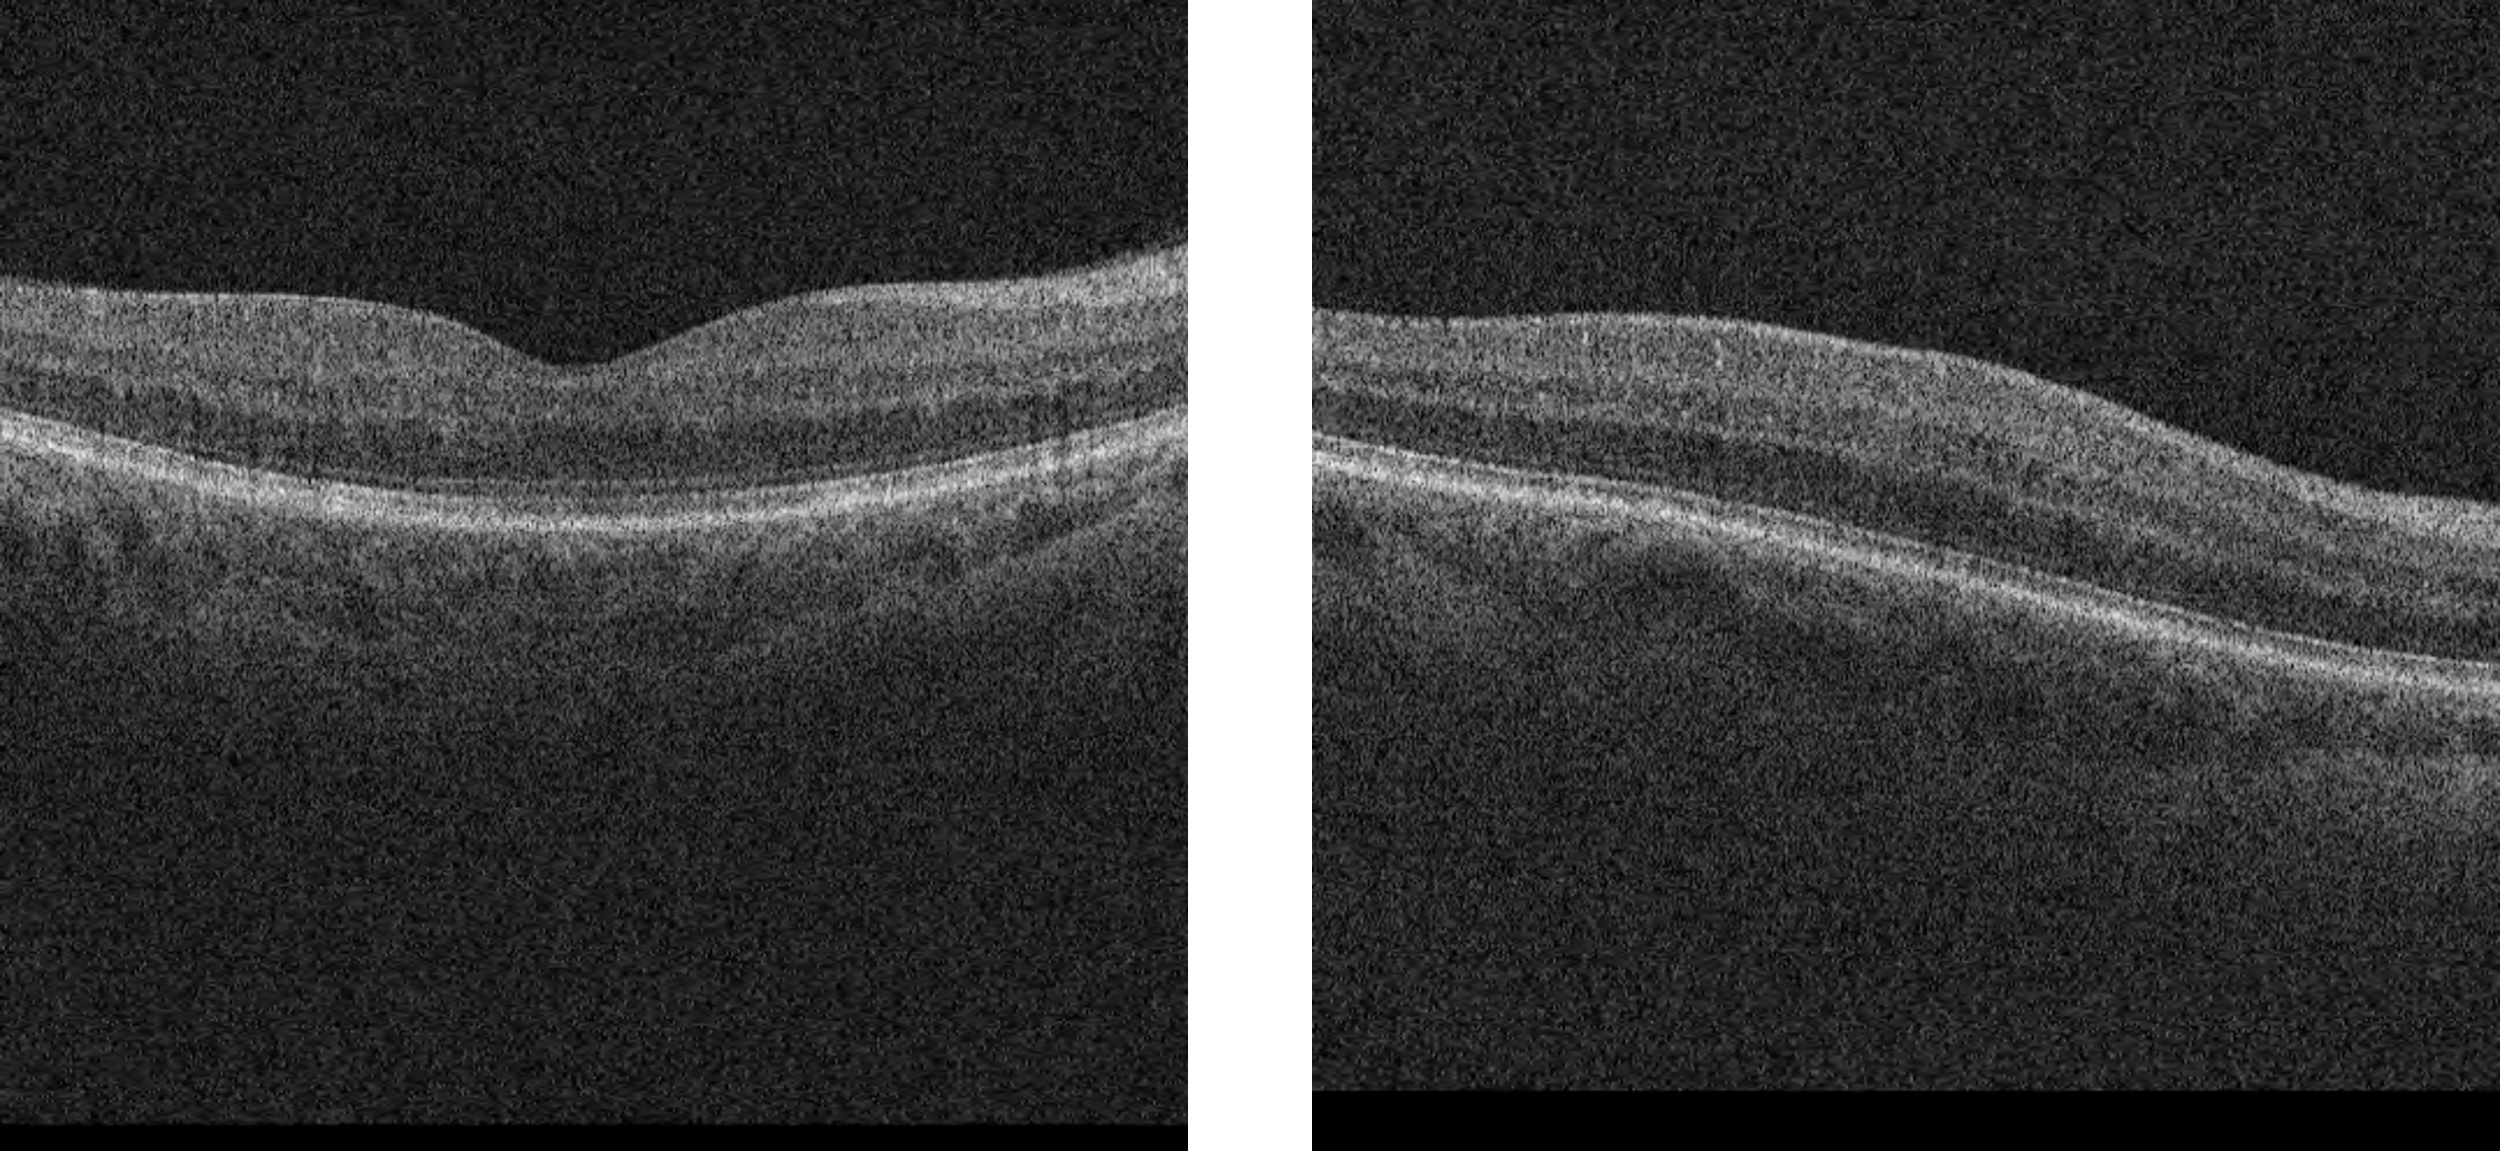
\includegraphics[width=0.7\linewidth]{figures/DifferentRetinaOrientation.png}
	\caption{Example of two B-scans in which the retina is oriented differently. The retina present in the right image is significantly more inclined. Both B-scans were obtained using a Cirrus device and do not present fluid.}
	\label{fig:DifferentRetinaOrientation}
\end{figure}

\begin{figure}[!ht]
	\centering
	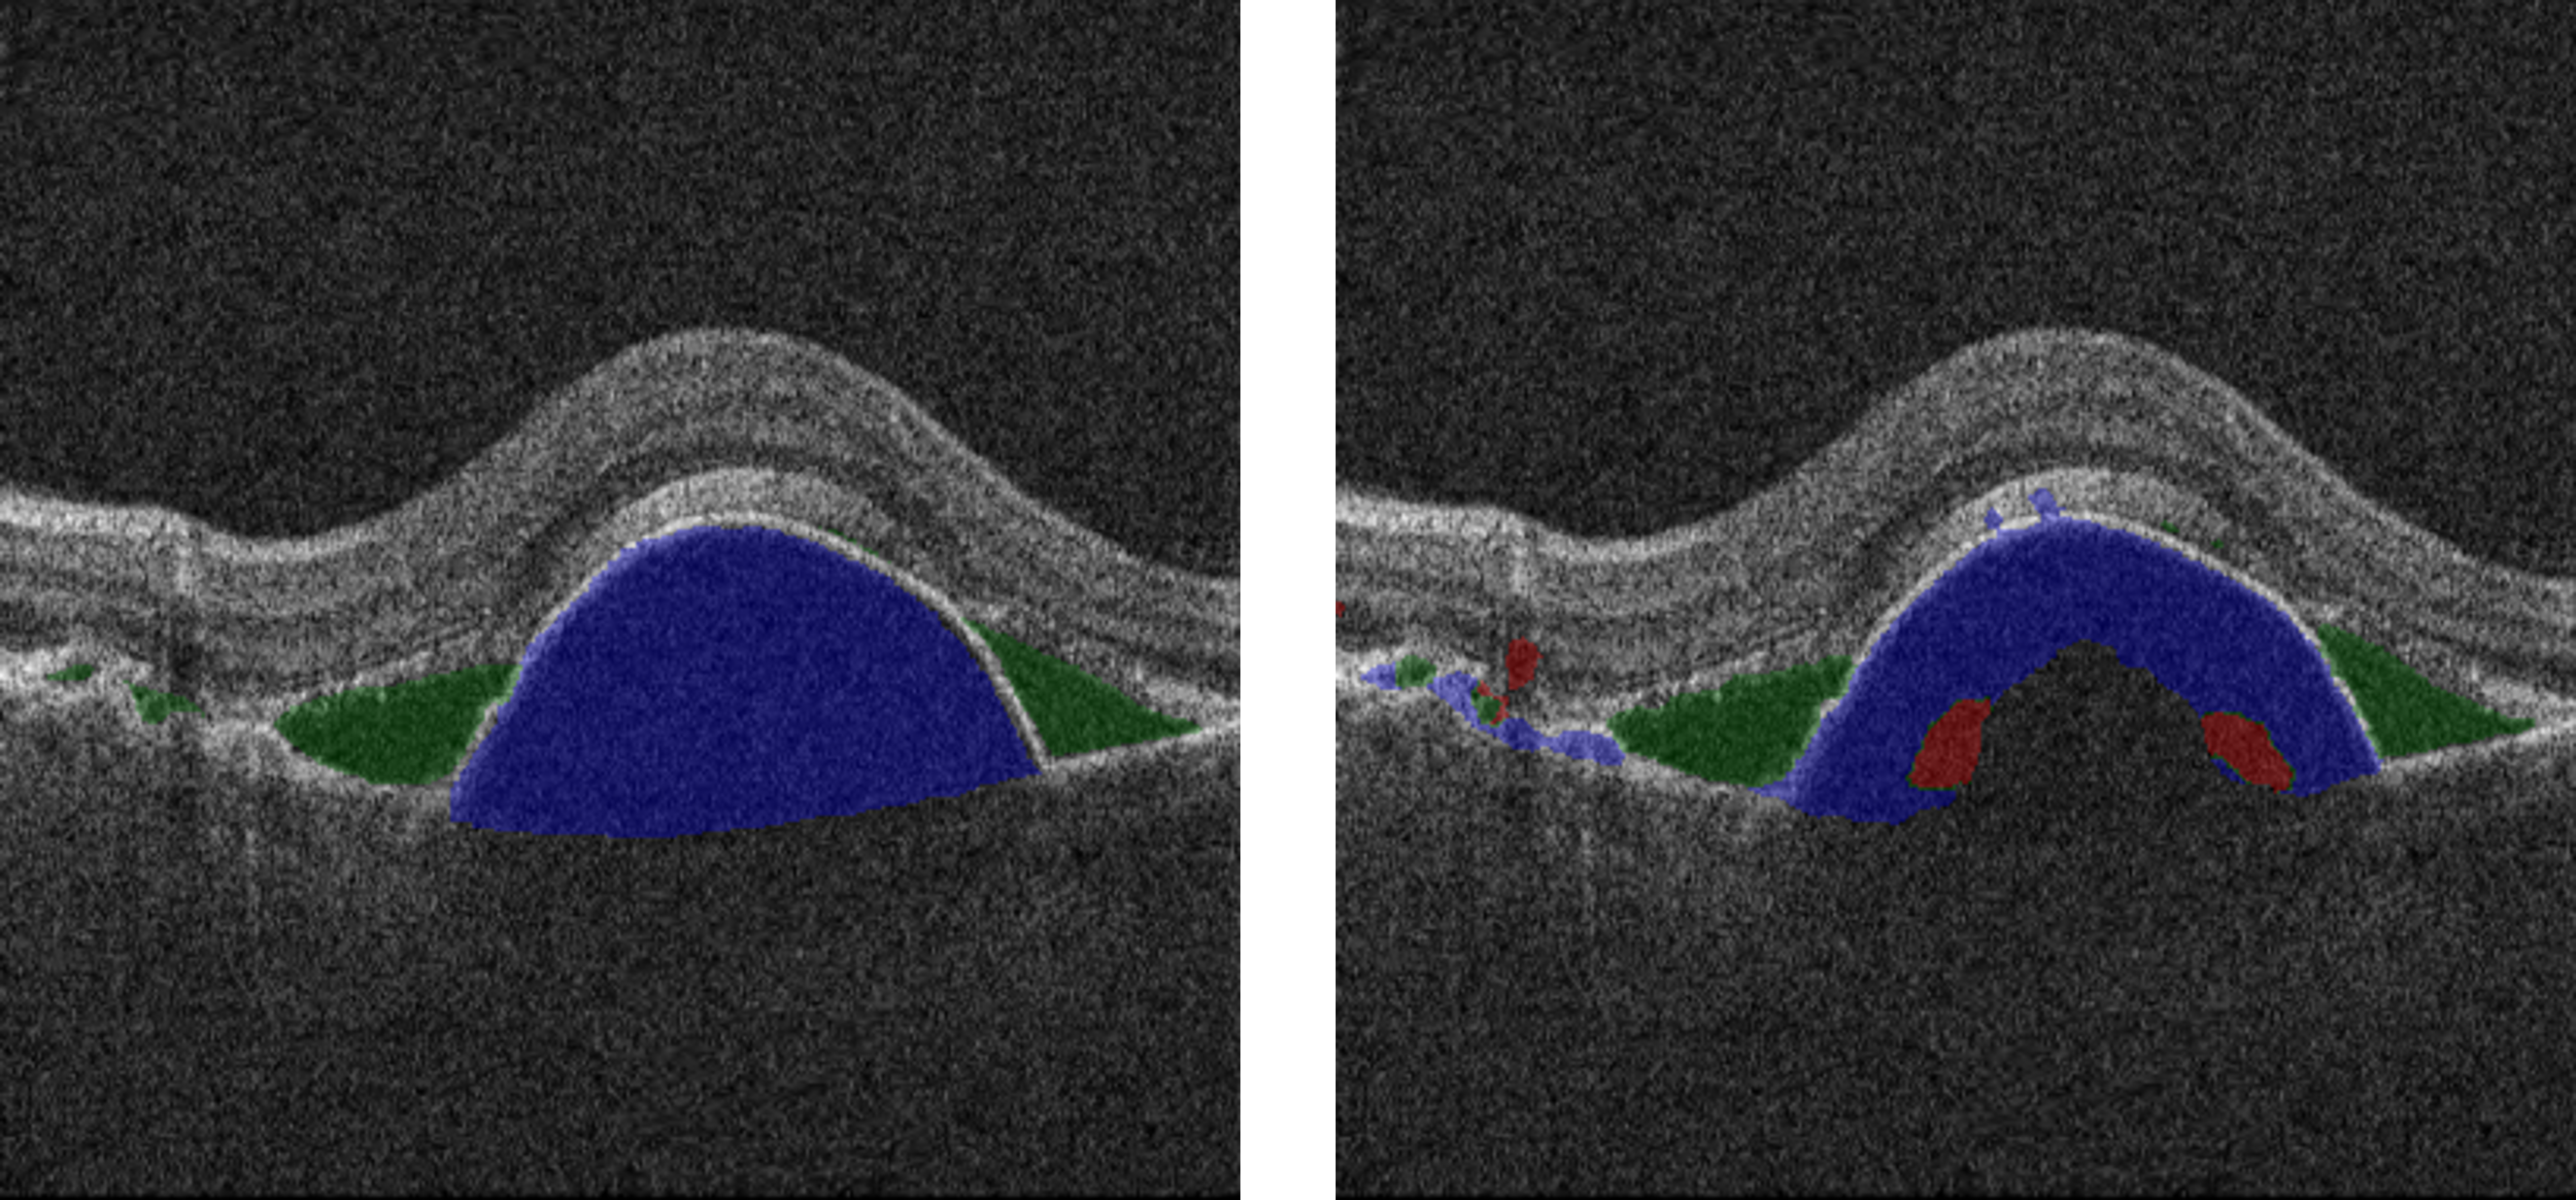
\includegraphics[width=0.7\linewidth]{figures/SegmentationErrorsNoRotation.png}
	\caption{Segmentation errors in Cirrus B-scans when trained without random rotations, in the same B-scan as in Figure \ref{fig:CirrusSegmentationErrors}. In the left, the GT masks are shown, while in the right the predicted masks are exhibited.}
	\label{fig:SegmentationErrorsNoRotation}
\end{figure}

In order to find an equilibrium between the robustness that training a model with rotated patches brings and the respect for the vertical order and relationships of the fluids, new runs were performed with a maximum $5^{\circ}$ rotation combined with the horizontal flipping. This rotation does not remove as much information from the patches as a $10^{\circ}$ rotation. The results obtained in these runs are shown in Table \ref{tab:Experiment1.3SevenPatches5DegreeRotation}.

\begin{table*}[!ht]
	\caption{Dice scores for every vendor and fluid using seven vertical patches. In these runs, horizontal flipping and $5^{\circ}$ rotation were used, instead of the usual $10^{\circ}$. The results obtained in Runs 21 and 22 are also shown, enabling a smoother comparison.}
	\centering
	\resizebox{\textwidth}{!}{\begin{tabular}{|c|c|ccc|ccc|ccc|c|c|c|c|}
		\hline
		% Headers
		\multirow{2}{*}{\textbf{Runs}} & 
		\multirow{2}{*}{\textbf{VF}} & 
		\multicolumn{3}{c|}{\textbf{Cirrus}} & 
		\multicolumn{3}{c|}{\textbf{Spectralis}} & 
		\multicolumn{3}{c|}{\textbf{Topcon}} & 
		\multicolumn{1}{c|}{\multirow{2}{*}{\textbf{IRF}}} & 
		\multirow{2}{*}{\textbf{SRF}} & 
		\multirow{2}{*}{\textbf{PED}} & 
		\multirow{2}{*}{\textbf{Fluid}} \\ \cline{3-11} & &
		\multicolumn{1}{c}{\textbf{IRF}} & 
		\multicolumn{1}{c}{\textbf{SRF}} & 
		\textbf{\textbf{PED}} & 
		\multicolumn{1}{c}{\textbf{IRF}} & 
		\multicolumn{1}{c}{\textbf{SRF}} & 
		\textbf{PED} & 
		\textbf{IRF} & 
		\textbf{SRF} & 
		\textbf{PED} & 
		\multicolumn{1}{c|}{} & & & \\ 
		
		\hline
		
		\textbf{Run 29} & 2 & \multicolumn{1}{c|}{0.497} & \multicolumn{1}{c|}{0.783} & 0.609 & \multicolumn{1}{c|}{0.763} & \multicolumn{1}{c|}{0.851} & 0.822 & \multicolumn{1}{c|}{0.832} & \multicolumn{1}{c|}{\textbf{0.904}} & 0.799 & 0.658 & 0.836 & 0.712 & 0.666 \\
		
		\textbf{Run 30} & 3 & \multicolumn{1}{c|}{0.475} & \multicolumn{1}{c|}{0.747} & 0.613 & \multicolumn{1}{c|}{0.656} & \multicolumn{1}{c|}{0.846} & 0.757 & \multicolumn{1}{c|}{\textbf{0.856}} & \multicolumn{1}{c|}{0.869} & \textbf{0.835} & 0.646 & 0.809 & 0.720 & 0.646 \\
		
		\textbf{Run 31} & 4 & \multicolumn{1}{c|}{0.643} & \multicolumn{1}{c|}{0.709} & 0.747 & \multicolumn{1}{c|}{0.627} & \multicolumn{1}{c|}{0.800} & 0.635 & \multicolumn{1}{c|}{0.457} & \multicolumn{1}{c|}{0.599} & 0.529 & 0.560 & 0.673 & 0.638 & 0.523 \\
		
		\textbf{Run 32} & 0 & \multicolumn{1}{c|}{\textbf{0.794}} & \multicolumn{1}{c|}{\textbf{0.878}} & \textbf{0.770} & \multicolumn{1}{c|}{\textbf{0.807}} & \multicolumn{1}{c|}{\textbf{0.902}} & \textbf{0.862} & \multicolumn{1}{c|}{0.796} & \multicolumn{1}{c|}{0.842} & 0.830 & \textbf{0.797} & \textbf{0.869} & \textbf{0.808} & \textbf{0.698} \\
		
		\hline
		
		\textbf{Set 7} & - & \multicolumn{1}{c|}{0.60} & \multicolumn{1}{c|}{0.78} & 0.68 & \multicolumn{1}{c|}{0.71} & \multicolumn{1}{c|}{0.85} & 0.77 & \multicolumn{1}{c|}{0.74} & \multicolumn{1}{c|}{0.80} & 0.75 & 0.67 & 0.80 & 0.72 & 0.63 \\
		
		\hline
		\hline
		
		\textbf{Run 21} & 2 & \multicolumn{1}{c|}{0.556} & \multicolumn{1}{c|}{0.837} & 0.672 & \multicolumn{1}{c|}{0.761} & \multicolumn{1}{c|}{0.853} & 0.848 & \multicolumn{1}{c|}{0.829} & \multicolumn{1}{c|}{0.908} & 0.858 & 0.685 & 0.864 & 0.767 & 0.681 \\

		\textbf{Run 22} & 3 & \multicolumn{1}{c|}{0.734} & \multicolumn{1}{c|}{0.855} & 0.836 & \multicolumn{1}{c|}{0.636} & \multicolumn{1}{c|}{0.846} & 0.689 & \multicolumn{1}{c|}{0.686} & \multicolumn{1}{c|}{0.781} & 0.731 & 0.700 & 0.822 & 0.771 & 0.672 \\

		\hline
			
	\end{tabular}}
	\label{tab:Experiment1.3SevenPatches5DegreeRotation}
\end{table*}

When looking at the results in Table \ref{tab:Experiment1.3SevenPatches5DegreeRotation}, the runs trained using a maximum $10^{\circ}$ rotation attain a better Dice coefficient than those that are trained using $5^{\circ}$. However, it is important to also compare the performances only in the slices that have fluid, which are shown in Table \ref{tab:Experiment1.3SevenPatches5DegreeRotationFluid}.

\begin{table*}[!ht]
	\caption{Dice scores for every vendor and fluid using seven vertical patches. The mean scores are calculated only for the B-scans that contain that fluid. For example, Cirrus IRF is the mean of the IRF Dice coefficient across all the Cirrus slices in the validation fold that contain IRF. The transformations utilized were the same as in Table \ref{tab:Experiment1.3SevenPatches5DegreeRotation}.}
	\centering
	\resizebox{\textwidth}{!}{\begin{tabular}{|c|c|ccc|ccc|ccc|c|c|c|c|}
			\hline
			% Headers
			\multirow{2}{*}{\textbf{Runs}} & 
			\multirow{2}{*}{\textbf{VF}} & 
			\multicolumn{3}{c|}{\textbf{Cirrus}} & 
			\multicolumn{3}{c|}{\textbf{Spectralis}} & 
			\multicolumn{3}{c|}{\textbf{Topcon}} & 
			\multicolumn{1}{c|}{\multirow{2}{*}{\textbf{IRF}}} & 
			\multirow{2}{*}{\textbf{SRF}} & 
			\multirow{2}{*}{\textbf{PED}} & 
			\multirow{2}{*}{\textbf{Fluid}} \\ \cline{3-11} & &
			\multicolumn{1}{c}{\textbf{IRF}} & 
			\multicolumn{1}{c}{\textbf{SRF}} & 
			\textbf{\textbf{PED}} & 
			\multicolumn{1}{c}{\textbf{IRF}} & 
			\multicolumn{1}{c}{\textbf{SRF}} & 
			\textbf{PED} & 
			\textbf{IRF} & 
			\textbf{SRF} & 
			\textbf{PED} & 
			\multicolumn{1}{c|}{} & & & \\ 
			
			\hline
			
			\textbf{Run 29} & 2 & \multicolumn{1}{c|}{0.499} & \multicolumn{1}{c|}{0.730} & \textbf{0.603} & \multicolumn{1}{c|}{0.596} & \multicolumn{1}{c|}{0.854} & 0.583 & \multicolumn{1}{c|}{\textbf{0.696}} & \multicolumn{1}{c|}{0.629} & 0.577 & 0.575 & 0.731 & 0.588 & 0.645 \\

			
			\textbf{Run 30} & 3 & \multicolumn{1}{c|}{0.535} & \multicolumn{1}{c|}{0.675} & 0.584 & \multicolumn{1}{c|}{0.519} & \multicolumn{1}{c|}{0.837} & 0.592 & \multicolumn{1}{c|}{0.646} & \multicolumn{1}{c|}{\textbf{0.735}} & 0.605 & 0.561 & 0.721 & 0.595 & 0.623 \\
			

			\textbf{Run 31} & 4 & \multicolumn{1}{c|}{\textbf{0.691}} & \multicolumn{1}{c|}{0.637} & 0.602 & \multicolumn{1}{c|}{0.619} & \multicolumn{1}{c|}{\textbf{0.899}} & 0.623 & \multicolumn{1}{c|}{0.506} & \multicolumn{1}{c|}{0.651} & \textbf{0.656} & 0.603 & 0.709 & \textbf{0.635} & \textbf{0.646} \\
			
			
			\textbf{Run 32} & 0 & \multicolumn{1}{c|}{0.627} & \multicolumn{1}{c|}{\textbf{0.815}} & 0.590 & \multicolumn{1}{c|}{\textbf{0.705}} & \multicolumn{1}{c|}{0.808} & \textbf{0.646} & \multicolumn{1}{c|}{0.563} & \multicolumn{1}{c|}{0.489} & 0.521 & \textbf{0.627} & \textbf{0.761} & 0.585 & 0.645 \\

			
			\hline
			
			\textbf{Set 7} & - & \multicolumn{1}{c|}{0.61} & \multicolumn{1}{c|}{0.74} & 0.59 & \multicolumn{1}{c|}{0.65} & \multicolumn{1}{c|}{0.85} & 0.65 & \multicolumn{1}{c|}{0.58} & \multicolumn{1}{c|}{0.62} & 0.55 & 0.60 & 0.75 & 0.59 & 0.64 \\

			\hline
			\hline
			
			\textbf{Run 21} & 2 & \multicolumn{1}{c|}{0.626} & \multicolumn{1}{c|}{0.795} & 0.449 & \multicolumn{1}{c|}{0.681} & \multicolumn{1}{c|}{0.842} & 0.771 & \multicolumn{1}{c|}{0.613} & \multicolumn{1}{c|}{0.697} & 0.524 & 0.636 & 0.791 & 0.518 & 0.636 \\
			
			
			\textbf{Run 22} & 3 & \multicolumn{1}{c|}{0.720} & \multicolumn{1}{c|}{0.687} & 0.554 & \multicolumn{1}{c|}{0.653} & \multicolumn{1}{c|}{0.914} & 0.543 & \multicolumn{1}{c|}{0.569} & \multicolumn{1}{c|}{0.679} & 0.615 & 0.647 & 0.738 & 0.583 & 0.651 \\
			
			
			\hline
			
	\end{tabular}}
	\label{tab:Experiment1.3SevenPatches5DegreeRotationFluid}
\end{table*}

The results shown in Table \ref{tab:Experiment1.3SevenPatches5DegreeRotationFluid} depict comparable results between the models trained with rotations of $5^{\circ}$ and $10^{\circ}$ degrees. While the results still slightly favor those trained with $10^{\circ}$ rotation, the difference between models is much smaller than it was in Table \ref{tab:Experiment1.3SevenPatches5DegreeRotation}. The differences observed indicate that the Dice coefficient measured in the models trained with $10^{\circ}$ rotation leverage on the high capability of detecting fluid. 
\par
This model is particularly good at detecting which slices have and do not have fluid. When the model does not detect fluid in a slice that does not have fluid, the Dice coefficient for that slice is 1. Meanwhile, in case the slices do not have fluid but the model still detects fluid in them, the B-scan's Dice coefficient for that fluid is 0.
\par
Due to the large quantity of slices that do not have fluid, which is larger than the slices that have fluid, a segmentation model can considerably improve its Dice performance by enhancing its capability of detecting fluid. Despite the model trained with $5^{\circ}$ performing worse at detecting fluid, most of these wrongful predictions are just a small quantity of sparse pixels (less than 100 pixels in each $496 \times 512$ image).
\par
It is also of interest to look into the predictions made by each model. While the Dice coefficient is a good metric to represent the models performance, some relevant segmentation characteristics can not be expressed by this measurement.
\par
When looking at the predictions made by both models, the model trained with $5^{\circ}$ rotations attains performances that are closer to the GT. An example of this can be seen in Figure \ref{fig:SegmentationsComparisonBetweenDifferentRotations}, where a comparison between the predictions made by different models are shown. In this image, it is seen that the masks predicted (middle image) by the model trained with $10^{\circ}$ rotation segments all the PED region, but also segments much more PED overall. Meanwhile, the model trained with $5^{\circ}$ rotation also identifies the PED region correctly, but segments less PED in the image (right image). The segmentation of IRF and SRF are really similar between both models.

\begin{figure}[!ht]
	\centering
	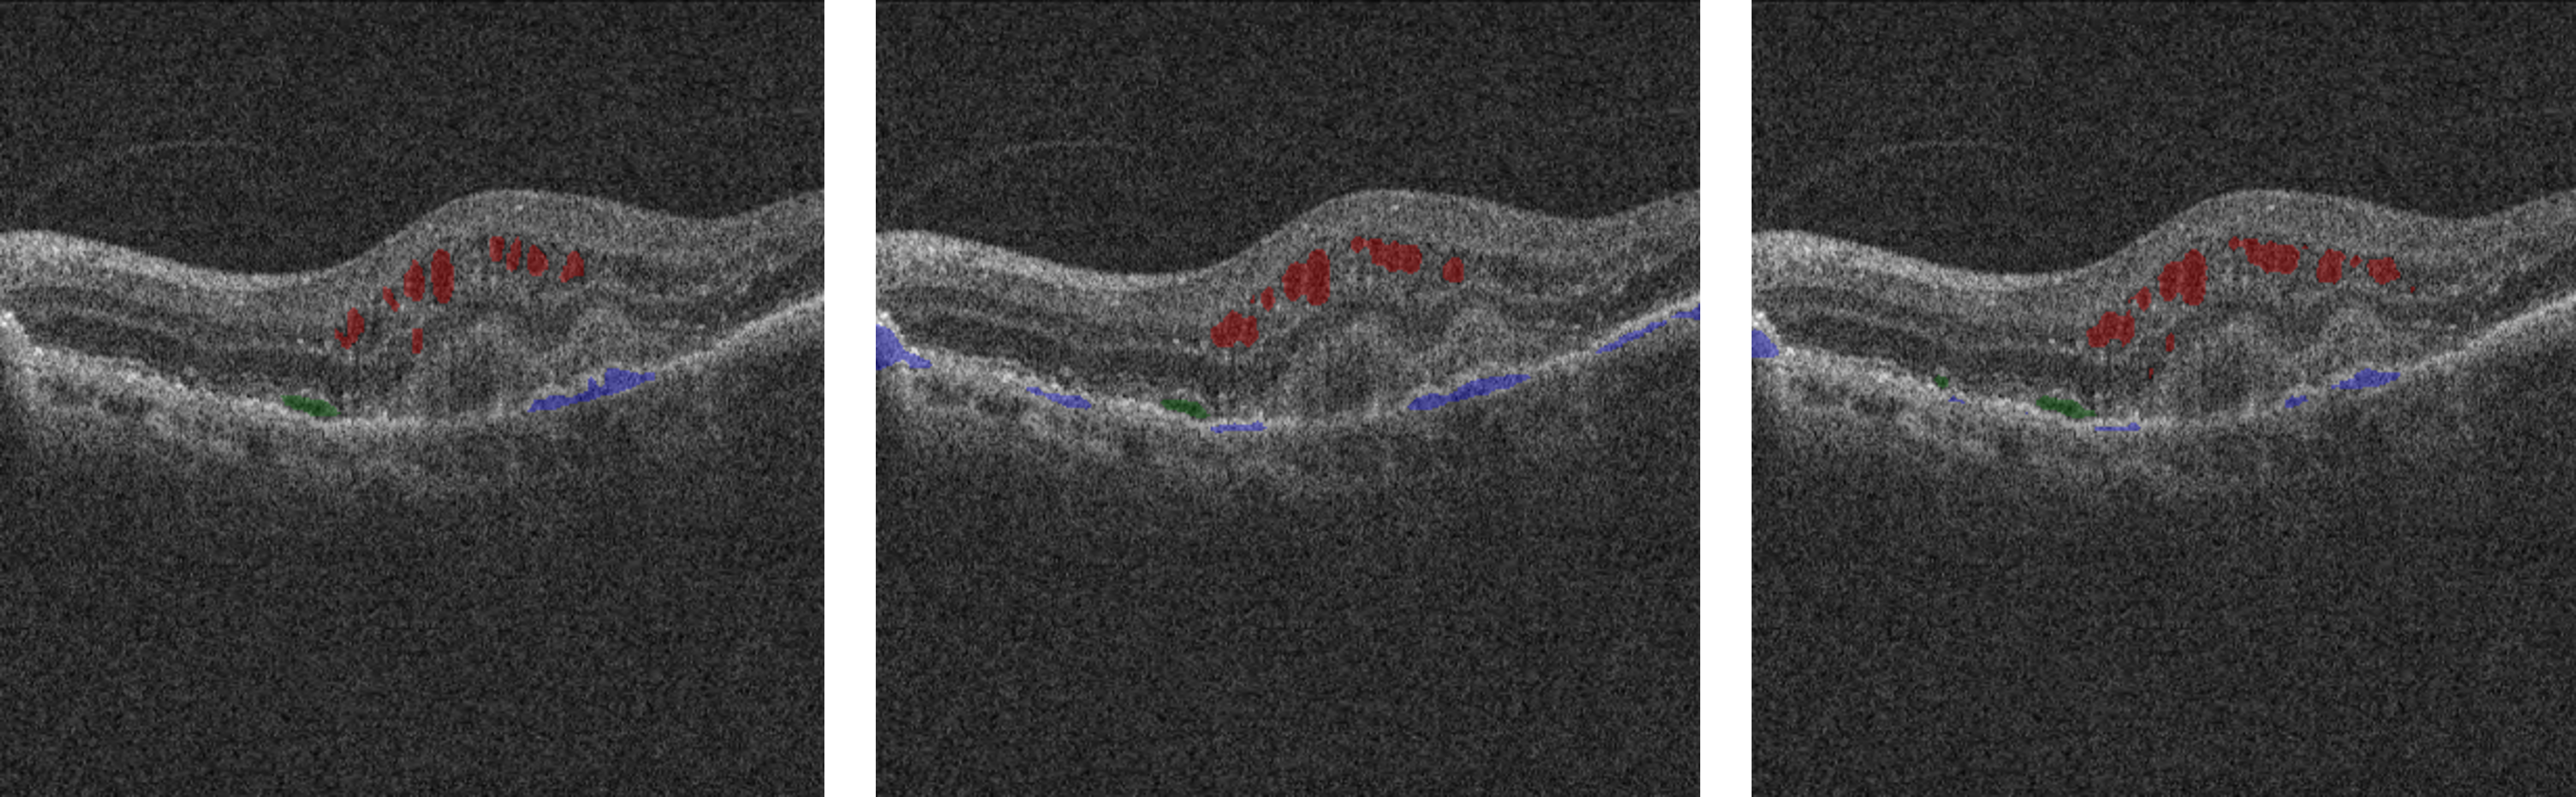
\includegraphics[width=1.0\linewidth]{figures/SegmentationsComparisonBetweenDifferentRotations.png}
	\caption{Predictions by the models trained using $5^{\circ}$ (middle image) and $10^{\circ}$ (right image) rotations, compared with the respective GT (left image).}
	\label{fig:SegmentationsComparisonBetweenDifferentRotations}
\end{figure}

This is an example of how the model trained with $5^{\circ}$ rotations tends to be more conservative in the fluid segmentation, despite not being as good at identifying fluid in the B-scans. For this reason, it was expected that this model would perform better on unseen data than the model trained with $10^{\circ}$ which tends to oversegment. Therefore, the maximum rotation selected for further experiments was $5^{\circ}$.
\par
Following the experiments that applied a $5^{\circ}$ rotation to the seven vertical patches extracted from each B-scan, additional runs were made using the same rotation, but with only four patches extracted from each B-scan instead. The objective of these runs was to verify if model still performs better on seven patches than on four patches when the applied rotation is changed from $10^{\circ}$ to $5^{\circ}$. The results are shown in Table \ref{tab:Experiment1.3FourPatches5DegreeRotation}.

\begin{table*}[!ht]
	\caption{Dice scores for every vendor and fluid using four vertical patches. The rotation applied in these runs was of $5^{\circ}$, instead of the previously used $10^{\circ}$. ``Set 7'' and the best performing run in this set (Run 32) are also shown, promoting an easier comparison between the use of four and seven patches. The underlined values correspond to the best performances between the models trained in Run 32 and Run 33.}
	\centering
	\resizebox{\textwidth}{!}{\begin{tabular}{|c|c|ccc|ccc|ccc|c|c|c|c|}
		\hline
		% Headers
		\multirow{2}{*}{\textbf{Runs}} & 
		\multirow{2}{*}{\textbf{VF}} & 
		\multicolumn{3}{c|}{\textbf{Cirrus}} & 
		\multicolumn{3}{c|}{\textbf{Spectralis}} & 
		\multicolumn{3}{c|}{\textbf{Topcon}} & 
		\multicolumn{1}{c|}{\multirow{2}{*}{\textbf{IRF}}} & 
		\multirow{2}{*}{\textbf{SRF}} & 
		\multirow{2}{*}{\textbf{PED}} & 
		\multirow{2}{*}{\textbf{Fluid}} \\ \cline{3-11} & &
		\multicolumn{1}{c}{\textbf{IRF}} & 
		\multicolumn{1}{c}{\textbf{SRF}} & 
		\textbf{\textbf{PED}} & 
		\multicolumn{1}{c}{\textbf{IRF}} & 
		\multicolumn{1}{c}{\textbf{SRF}} & 
		\textbf{PED} & 
		\textbf{IRF} & 
		\textbf{SRF} & 
		\textbf{PED} & 
		\multicolumn{1}{c|}{} & & & \\ 
			
		\hline
		
		\textbf{Run 33} & 2 & \multicolumn{1}{c|}{0.598} & \multicolumn{1}{c|}{\textbf{0.824}} & 0.719 & \multicolumn{1}{c|}{\textbf{0.805}} & \multicolumn{1}{c|}{0.873} & \underline{\textbf{0.887}} & \multicolumn{1}{c|}{\underline{\textbf{0.848}}} & \multicolumn{1}{c|}{\underline{\textbf{0.947}}} & \underline{\textbf{0.863}} & \textbf{0.720} & \underline{\textbf{0.874}} & \textbf{0.798} & \underline{\textbf{0.733}} \\
		
		\textbf{Run 34} & 3 & \multicolumn{1}{c|}{0.298} & \multicolumn{1}{c|}{0.701} & 0.436 & \multicolumn{1}{c|}{0.442} & \multicolumn{1}{c|}{0.785} & 0.720 & \multicolumn{1}{c|}{0.717} & \multicolumn{1}{c|}{0.814} & 0.746 & 0.477 & 0.757 & 0.599 & 0.530 \\
		
		\textbf{Run 35} & 4 & \multicolumn{1}{c|}{0.670} & \multicolumn{1}{c|}{0.796} & \textbf{0.850} & \multicolumn{1}{c|}{0.531} & \multicolumn{1}{c|}{0.825} & 0.701 & \multicolumn{1}{c|}{0.509} & \multicolumn{1}{c|}{0.703} & 0.674 & 0.582 & 0.759 & 0.754 & 0.578 \\
		
		\textbf{Run 36} & 0 & \multicolumn{1}{c|}{\textbf{0.695}} & \multicolumn{1}{c|}{0.816} & 0.737 & \multicolumn{1}{c|}{0.761} & \multicolumn{1}{c|}{\textbf{0.882}} & 0.838 & \multicolumn{1}{c|}{0.728} & \multicolumn{1}{c|}{0.867} & 0.775 & 0.719 & 0.846 & 0.769 & 0.635 \\
		
		\hline
		
		\textbf{Set 8} & - & \multicolumn{1}{c|}{0.57} & \multicolumn{1}{c|}{\textbf{0.78}} & \textbf{0.69} & \multicolumn{1}{c|}{0.63} & \multicolumn{1}{c|}{0.84} & \textbf{0.79} & \multicolumn{1}{c|}{0.70} & \multicolumn{1}{c|}{\textbf{0.83}} & \textbf{0.76} & 0.62 & \textbf{0.81} & \textbf{0.73} & 0.62 \\
		
		\hline
		\hline
		
		\textbf{Run 32} & 0 & \multicolumn{1}{c|}{\underline{0.794}} & \multicolumn{1}{c|}{\underline{0.878}} & \underline{0.770} & \multicolumn{1}{c|}{\underline{0.807}} & \multicolumn{1}{c|}{\underline{0.902}} & 0.862 & \multicolumn{1}{c|}{0.796} & \multicolumn{1}{c|}{0.842} & 0.830 & \underline{0.797} & 0.869 & \underline{0.808} & 0.698 \\
		
		\hline
		
		\textbf{Set 7} & - & \multicolumn{1}{c|}{\textbf{0.60}} & \multicolumn{1}{c|}{\textbf{0.78}} & 0.68 & \multicolumn{1}{c|}{\textbf{0.71}} & \multicolumn{1}{c|}{\textbf{0.85}} & 0.77 & \multicolumn{1}{c|}{\textbf{0.74}} & \multicolumn{1}{c|}{0.80} & 0.75 & \textbf{0.67} & 0.80 & 0.72 & \textbf{0.63} \\
		
		\hline
			
	\end{tabular}}
	\label{tab:Experiment1.3FourPatches5DegreeRotation}
\end{table*}

Contrasting with the results shown in Table \ref{tab:Experiment1.3FourPatches} and Table \ref{tab:Experiment1.3SevenVsThirteenPatches}, which show a significant improvement when using seven vertical patches over four, the results exhibited in Table \ref{tab:Experiment1.3FourPatches5DegreeRotation} present a similar performance between the models trained on four and seven vertical patches. The main performance differences are in the IRF segmentation, where the difference is more significant depending on the number of patches used, favoring the models trained with seven patches.
\par
However, it is necessary to select a single segmentation model to perform inference in the fold that was reserved. The best performing model from those trained with seven vertical patches obtained from each B-scan and a maximum rotation of $5^{\circ}$ is the model trained in Run 32. Meanwhile, the best performing model from ``Set 8'' is Run 33. In Table \ref{tab:Experiment1.3FourPatches5DegreeRotation}, the underlined values correspond to the best performance attained between Run 32 and 33.
\par
In most metrics, the model trained on Run 32 performs better than the model trained on Run 33. Nevertheless, both performances are really similar in most metrics, with the only significant difference being the IRF segmentation, which is superior in Run 32. It is important to note that the models were nor trained nor validated on the same data and an assumption that this would directly translate to the performance in unseen data was made. However, it is possible that the data in which one model was trained prepares it better for the data on the reserved fold. Therefore, the U-Net model selected to represent the multi-class segmentation approach was the one trained in Run 32. This model subsequently performed the inference in the unseen fold (fold 1) and its results are shown in Table \ref{tab:Experiment1.3FinalResults}. In this table, the rows correspond to the model performances on different sets of slices. In the first row the performance across all slices is considered. In the second row only the slices with the fluid indicated in the column are quantified, while in the third row only those that do not present that fluid are considered.

\begin{table*}[!ht]
	\caption{Dice scores for every vendor and fluid in the reserved fold (fold 1). The first row reports the mean Dice across all slices. The second row shows the mean for slices containing the fluid specified in the column, while the third shows the mean for the slices without that fluid.}
	\centering
	\resizebox{\textwidth}{!}{\begin{tabular}{|c|c|c|ccc|ccc|ccc|c|c|c|c|}
		\hline
		% Headers
		\multirow{2}{*}{\textbf{Runs}} &
		\multirow{2}{*}{\textbf{Slices}} &  
		\multirow{2}{*}{\textbf{VF}} & 
		\multicolumn{3}{c|}{\textbf{Cirrus}} & 
		\multicolumn{3}{c|}{\textbf{Spectralis}} & 
		\multicolumn{3}{c|}{\textbf{Topcon}} & 
		\multicolumn{1}{c|}{\multirow{2}{*}{\textbf{IRF}}} & 
		\multirow{2}{*}{\textbf{SRF}} & 
		\multirow{2}{*}{\textbf{PED}} & 
		\multirow{2}{*}{\textbf{Fluid}} \\ \cline{4-12} & & &
		\multicolumn{1}{c}{\textbf{IRF}} & 
		\multicolumn{1}{c}{\textbf{SRF}} & 
		\textbf{\textbf{PED}} & 
		\multicolumn{1}{c}{\textbf{IRF}} & 
		\multicolumn{1}{c}{\textbf{SRF}} & 
		\textbf{PED} & 
		\textbf{IRF} & 
		\textbf{SRF} & 
		\textbf{PED} & 
		\multicolumn{1}{c|}{} & & & \\ 
			
		\hline
			
		\multirow{3}{*}{\textbf{Run 32}} & All & 1 & \multicolumn{1}{c|}{0.852} & \multicolumn{1}{c|}{0.918} & 0.934 & \multicolumn{1}{c|}{0.645} & \multicolumn{1}{c|}{0.821} & 0.852 & \multicolumn{1}{c|}{0.818} & \multicolumn{1}{c|}{0.929} & 0.755 & 0.799 & 0.905 & 0.841 & 0.742 \\
		
		& Fluid & 1 & \multicolumn{1}{c|}{0.654} & \multicolumn{1}{c|}{0.799} & 0.767 & \multicolumn{1}{c|}{0.645} & \multicolumn{1}{c|}{0.687} & 0.703 & \multicolumn{1}{c|}{0.624} & \multicolumn{1}{c|}{0.744} & 0.588 & 0.641 & 0.756 & 0.716 & 0.702 \\
		
		& No Fluid & 1 & \multicolumn{1}{c|}{0.941} & \multicolumn{1}{c|}{0.972} & 0.978 & \multicolumn{1}{c|}{0.646} & \multicolumn{1}{c|}{0.889} & 0.885 & \multicolumn{1}{c|}{0.884} & \multicolumn{1}{c|}{0.960} & 0.766 & 0.873 & 0.952 & 0.862 & 0.786 \\
		
		\hline
			
	\end{tabular}}
	\label{tab:Experiment1.3FinalResults}
\end{table*}

The results shown in the table indicate that the model generalized well. The performance obtained in the reserved fold, whose data had not been used in training or validation, reveals the model's robustness across different fluids and vendors. Since the model performs equally well across the three vendors, a good cross-device generalization has been achieved. Therefore, the model is not dependent on the image quality of the B-scans to produce accurate predictions.
\par
The model behaved differently depending on the fluid expected to segment. The Dice coefficient was considerably larger in SRF and PED than in IRF. This is associated with the larger variety of IRF shape and position in the retina. IRF regions are usually irregular in shape, smaller, and less well-defined than the other fluids, often appearing as small structures. This fluid is also located between the retinal layers, making it harder for the model to distinguish from the surrounding tissue and often leading to labeling ambiguity. Still, the model attained a better performance in fluid segmentation than those seen in Table \ref{tab:Experiment1.3SevenPatches5DegreeRotationFluid}, where only fluid is considered.
\par
When considering all the slices, the Dice coefficient improves significantly, when compared to its performance where only slices with fluid are considered. At the same time, the Dice coefficient obtained in the slices without fluid is also better than the fluid segmentation. This reflects the greater difficulty of accurately segmenting the fluids, when compared to the task of detecting their presence. Since most slices in the dataset do not present fluid, an accurate detection of it can significantly increase the Dice mean across all slices, as explained previously.
\par
Overall, the performance obtained when validating in this unseen fold is significantly better than any other validation performance in previously seen in Table \ref{tab:Experiment1.3SevenPatches5DegreeRotation}. This indicates that the model did not overfit on training data, benefiting from the diversity introduced in training both through varying images and the transformations applied to them. This performance also benefits from selecting the best performing model in cross-validation, which allows the choice of a robust model. 
\par
In Figures \ref{fig:Experiment1FinalModelPredictionsCirrus}, \ref{fig:Experiment1FinalModelPredictionsSpectralis}, and \ref{fig:Experiment1FinalModelPredictionsTopcon}, some examples of predictions performed by the model in the unseen data are shown. In the IRF segmentations, it is seen that the model can not correctly identify the retinal tissue that separates the fluid regions and connects nearby fluid regions. The PED segmentation is marked by accurate delimitation of the large PED regions, with some predictions made in B-scans without PED. Lastly, SRF is the fluid in which the prediction segmentation more resembles the GT.
\par
The performance seen by this model in the reserved fold was subsequently compared with the best performing models from the following experiment.

\begin{figure}[!ht]
	\centering
	\includegraphics[width=0.9\linewidth]{figures/Experiment1FinalModelPredictionsCirrus.png}
	\caption{Predictions by the model trained on Run 32 in unseen Cirrus volumes of fold 1.}
	\label{fig:Experiment1FinalModelPredictionsCirrus}
\end{figure}

\begin{figure}[!ht]
	\centering
	\includegraphics[width=0.9\linewidth]{figures/Experiment1FinalModelPredictionsSpectralis.png}
	\caption{Predictions by the model trained on Run 32 in unseen Spectralis volumes of fold 1.}
	\label{fig:Experiment1FinalModelPredictionsSpectralis}
\end{figure}

\begin{figure}[!ht]
	\centering
	\includegraphics[width=0.9\linewidth]{figures/Experiment1FinalModelPredictionsTopcon.png}
	\caption{Predictions by the model trained on Run 32 in unseen Topcon volumes of fold 1.}
	\label{fig:Experiment1FinalModelPredictionsTopcon}
\end{figure}

\subsection{Experiment 2}
The results shown in this subsection correspond to the use of three separate U-Nets, one for each fluid, to perform multi-class fluid segmentation. In Experiment 2.1, the loss function was the same as in Experiment 1, while in Experiment 2.2 the loss function was changed to the weighted cross-entropy. The results in these experiments were compared with each other.

\subsubsection{Experiment 2.1}
In this experiment, for each fluid, eight models were trained. One model was trained for each fold in the multi-class 5-fold split and then one model was trained for each fold in a fluid-specific 5-fold split.
\par
Table \ref{tab:Experiment2IRF} illustrates the performance of the models trained to segment IRF, with the upper block corresponding to the models trained on the multi-class split while the second block shows the performances for the models trained on the split specifically made for IRF segmentation.

\begin{table*}[!ht]
	\caption{IRF Dice scores for every vendor. Runs 37 to 40 utilize the multi-class 5-fold split from Experiment 1, while the Runs 41 to 44 use the fluid-specific 5-fold split. The results are presented both for every slice and for the slices which contain IRF.}
	\centering
	\begin{tabular}{|c|c|cc|cc|cc|cc|}
			\hline
			\multirow{2}{*}{\textbf{Runs}} &
			\multirow{2}{*}{\textbf{VF}} & 
			\multicolumn{2}{c|}{\textbf{Cirrus}} & 
			\multicolumn{2}{c|}{\textbf{Spectralis}} & 
			\multicolumn{2}{c|}{\textbf{Topcon}} & 
			\multicolumn{2}{c|}{\textbf{IRF}} \\ 
			\cline{3-10} & &
			\multicolumn{1}{c}{\textbf{All}} &  
			\textbf{\textbf{Fluid}} & 
			\multicolumn{1}{c}{\textbf{All}} &  
			\textbf{\textbf{Fluid}} & 
			\multicolumn{1}{c}{\textbf{All}} & 
			\textbf{\textbf{Fluid}} & 
			\multicolumn{1}{c}{\textbf{All}} & 
			\textbf{\textbf{Fluid}}\\ 
			
			\hline
			
			\textbf{Run 37} & 2 & 0.478 & 0.634 & 0.695 & 0.669 & 0.735 & 0.569 & 0.604 & 0.625 \\
			
			\textbf{Run 38} & 3 & 0.536 & 0.452 & 0.514 & 0.588 & \textbf{0.820} & \textbf{0.706} & 0.637 & 0.553 \\
			
			\textbf{Run 39} & 4 & 0.545 & \textbf{0.683} & 0.617 & 0.670 & 0.540 & 0.484 & 0.552 & 0.600 \\
			
			\textbf{Run 40} & 0 & 0.576 & 0.619 & 0.695 & 0.682 & 0.661 & 0.599 & 0.628 & 0.628 \\
			
			\hline
			
			\textbf{Set 9} & - & 0.53 & 0.60 & 0.63 & 0.65 & 0.69 & \textbf{0.59} & 0.61 & 0.60 \\
			
			\hline
			\hline
			
			\textbf{Run 41} & 2 & \textbf{0.654} & 0.663 & 0.541 & 0.606 & 0.648 & 0.619 & 0.632 & 0.635 \\
			
			\textbf{Run 42} & 3 & 0.507 & 0.641 & \textbf{0.741} & 0.670 & 0.775 & 0.675 & \textbf{0.649} & \textbf{0.656} \\
			
			\textbf{Run 43} & 4 & 0.583 & 0.516 & 0.689 & 0.660 & 0.310 & 0.451 & 0.502 & 0.546 \\
			
			\textbf{Run 44} & 0 & 0.618 & 0.566 & 0.644 & \textbf{0.686} & 0.588 & 0.600 & 0.611 & 0.594 \\
			
			\hline
			
			\textbf{Set 10} & - & 0.59 & 0.60 & 0.65 & \textbf{0.66} & 0.58 & \textbf{0.59} & 0.60 & \textbf{0.61} \\
			
			\hline
			\hline
			
			\textbf{Set 7} & - & \textbf{0.60} & \textbf{0.61} & \textbf{0.71} & 0.65 & \textbf{0.74} & 0.58 & \textbf{0.67} & 0.60 \\
			
			\hline
			
	\end{tabular}
	\label{tab:Experiment2IRF}
\end{table*}

The results shown in this table follow a well defined trend: the IRF segmentation in the slices which contain this fluid performs similarly to the segmentation predicted by multi-class models, while the performance when considering all the slices is significantly worse.
\par
The Dice obtained in segmentation in the slices with IRF is really similar to the values obtained when training multi-class models, as the difference between the mean of the runs performed is around 0.01 for all vendors. Changing the split in which the models were trained barely made a difference in the performances' average. However, while the segmentation in slices with IRF almost did not change, the mean performance in all the slices saw a significant improvement in Cirrus and a slight increase in Spectralis, combined with a significant decrease in Topcon. 
\par
The reason Topcon behaves differently is because, overall, the volumes obtained with devices from this vendor present less fluid than the volumes obtained with the other devices. Therefore, the model has to analyze the Topcon images more carefully and be more attentive of the smaller details, as the fluid regions are not as big as those seen in the other vendors. This leads to the model being better at separating the slices with fluid from those that do not present fluid. As seen in Experiment 1, an effective detection of fluid can significantly improve the model's Dice coefficient. The implications this has in model performance's are also visible in the multi-class segmentation results, as shown in the performance differences in B-scans from Topcon between Table \ref{tab:Experiment1.3SevenPatches5DegreeRotation} and Table \ref{tab:Experiment1.3SevenPatches5DegreeRotationFluid}.
\par
When comparing the results across all slices between these binary models with the multi-class, it is seen a significant decrease in Dice coefficient in the models tasked to segment exclusively IRF. There are two main causes for this decrease, with the first being an increment in the number of pixels labeled as background. As the model attempts to exclusively segment IRF, all the pixels that are not labeled as IRF, are classified as background. This means that the regions of SRF and PED are also interpreted as background. The images in the dataset are predominantly composed of non-fluid pixels, but, by re-assigning the other fluids' pixels in the retina as background, the proportion of fluid pixels in the image, and particularly in the retina, becomes even smaller. As the number of background pixels increase, the more chances the model has of mislabeling them as fluid.
\par
The increased number of background pixels is further impacted with the lack of inter-class competition. This inter-class competition is particularly helpful in the segmentation of other ambiguous regions such as other fluids, which, in binary segmentation, is not contested by other classes. This does not motivate the model to learn the anatomical characteristics of the retina that are key to identifying the region corresponding to each fluid, often leading to over-segmentation. 
\par
This translates to a decrease in the IRF segmentation model's performance, particularly in the slices that do not present this fluid, with two examples shown in Figure \ref{fig:Experiment2IRFSegmentation}. The same performance decrease is also seen in SRF and PED, as shown further, due to the same reasons.

\begin{figure}[!ht]
	\centering
	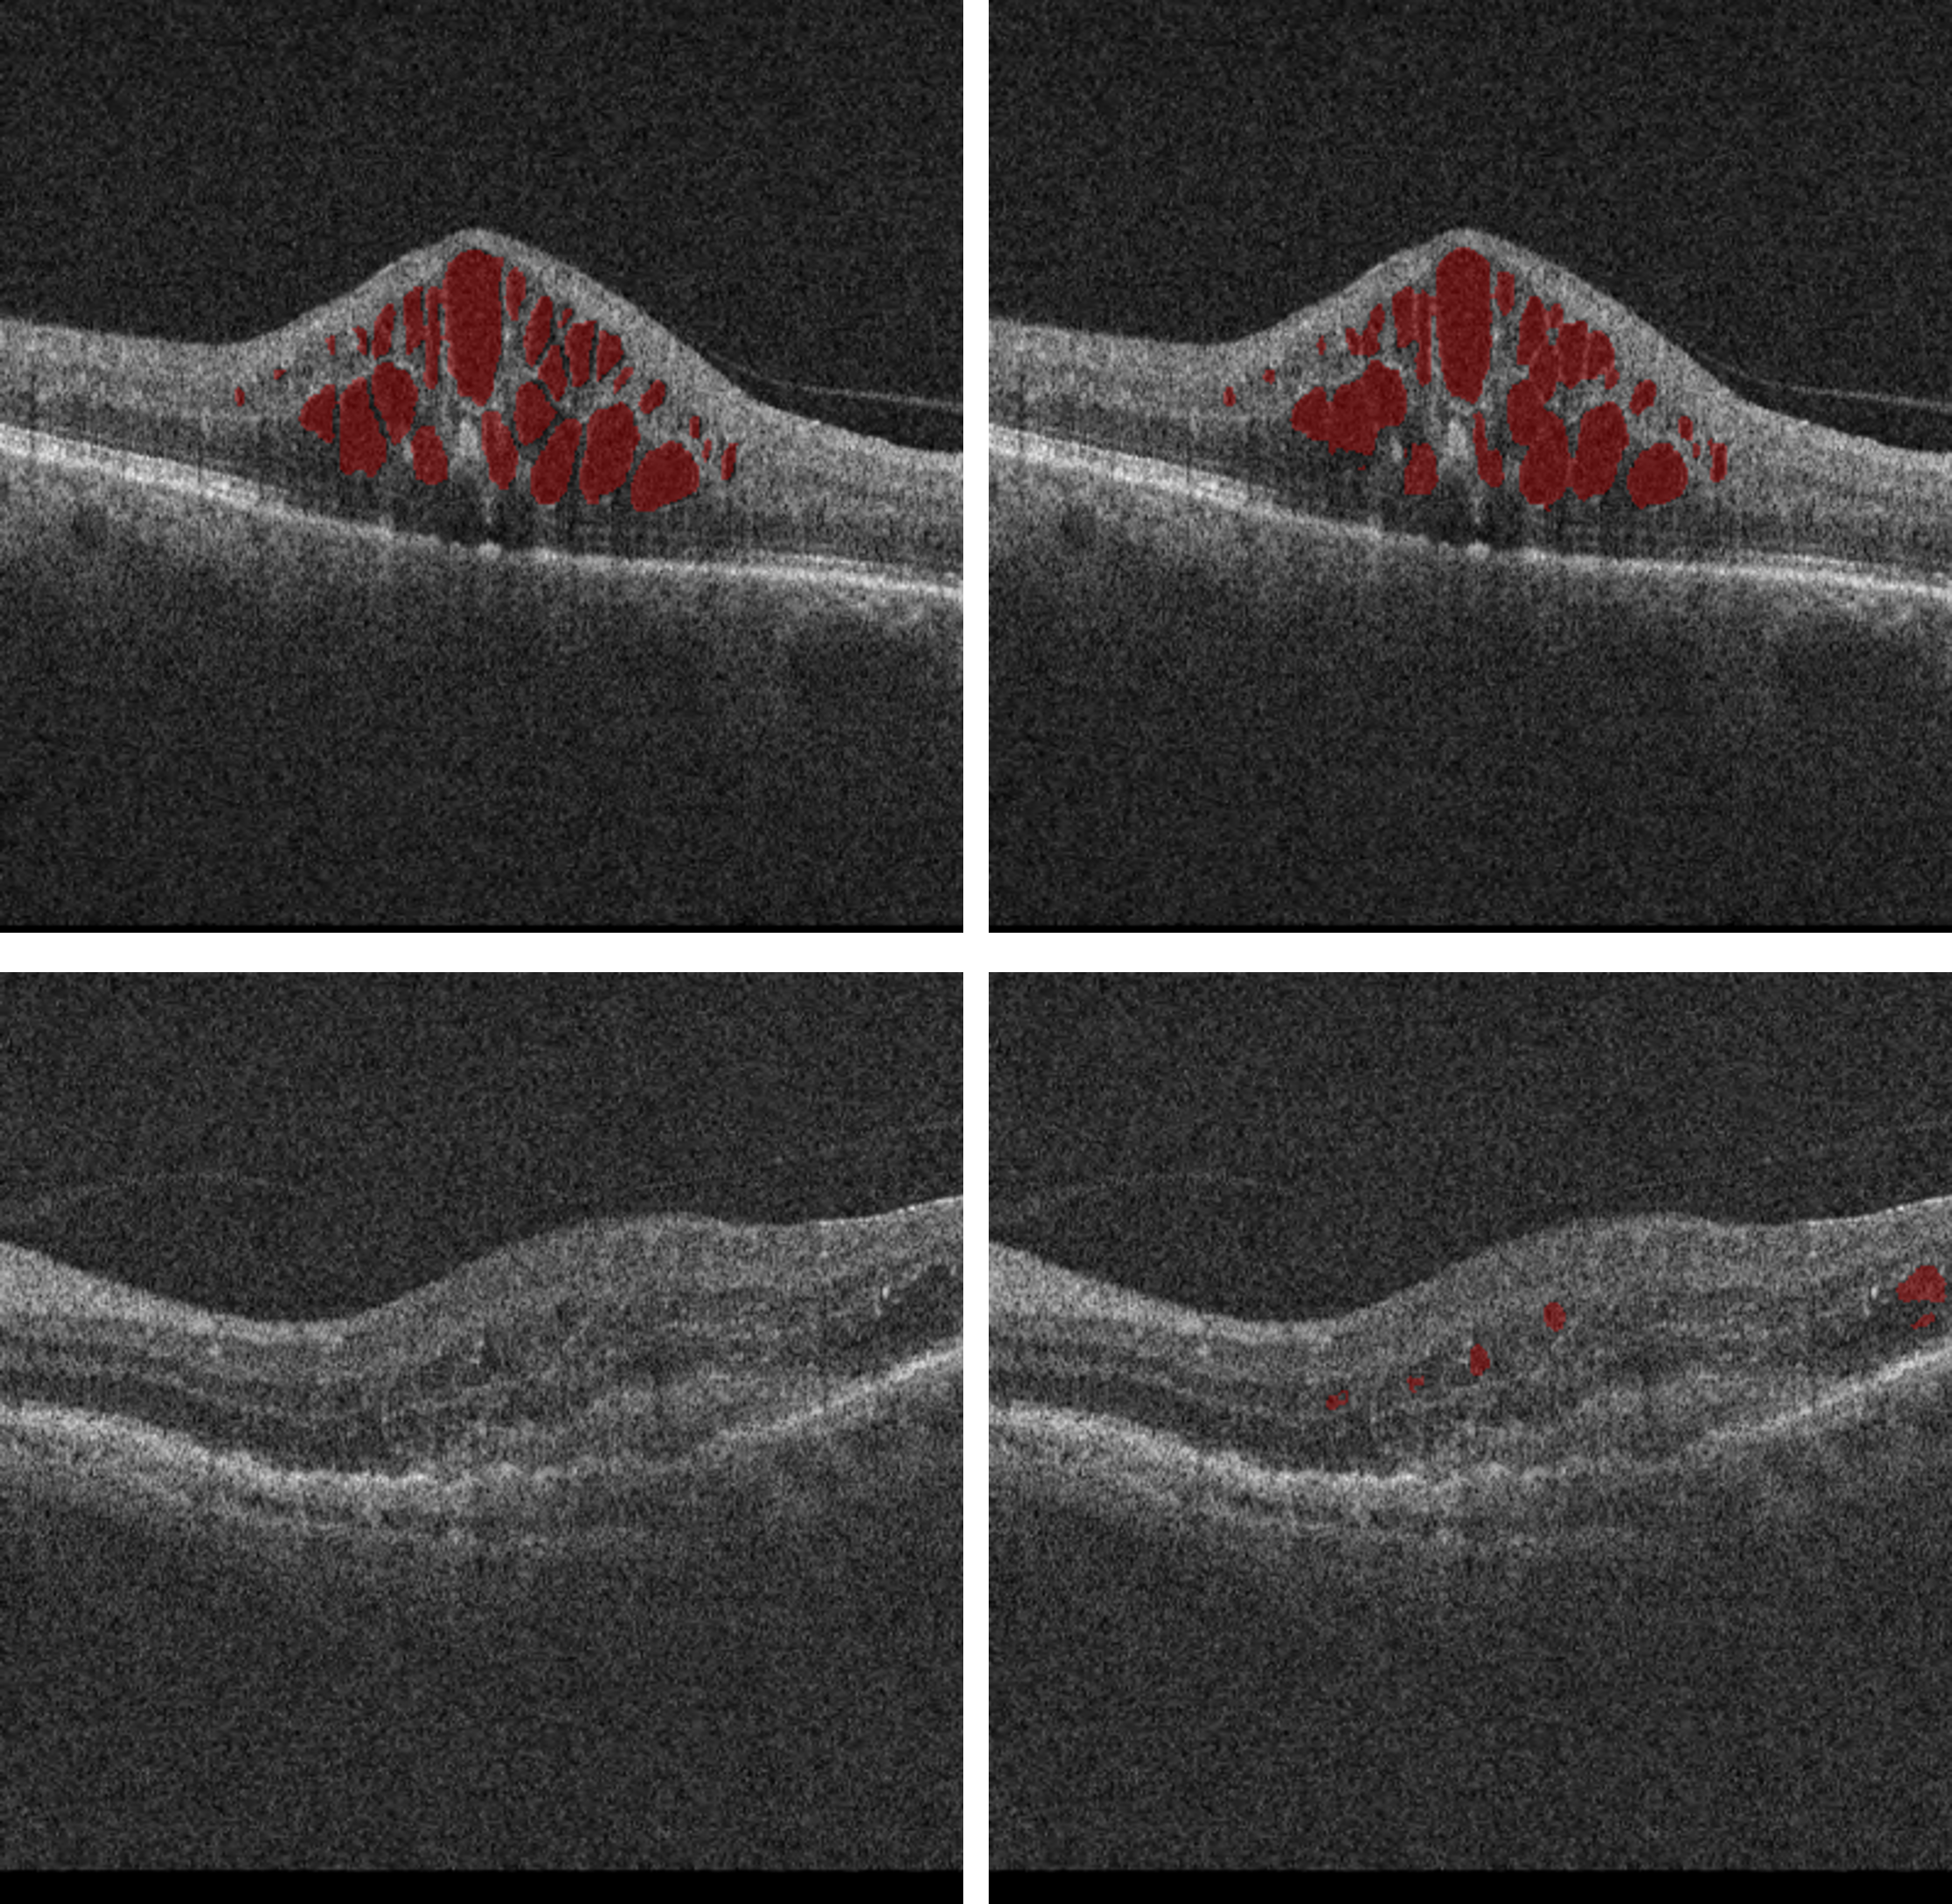
\includegraphics[width=0.7\linewidth]{figures/Experiment2IRFSegmentation.png}
	\caption{Predictions (right) performed by the binary IRF segmentation model and their respective GT (left). The prediction represented in the top show an example of an accurate IRF segmentation, while the bottom prediction reveals an oversegmentation in a slice that does not contain fluid.}
	\label{fig:Experiment2IRFSegmentation}
\end{figure}

Table \ref{tab:Experiment2SRF} shows the performance of the models trained on the same conditions as those trained to segment IRF, but now with the goal of segmenting SRF. Similarly, on the second block of this table, the models were trained using a 5-fold split specifically made to evenly distribute the OCT volumes according to the quantity of SRF in them.

\begin{table*}[!ht]
	\caption{SRF Dice scores for every vendor. Runs 45 to 48 utilize the multi-class 5-fold split from Experiment 1, while the Runs 49 to 52 use the fluid-specific 5-fold split. The results are presented both for every slice and for the slices which present SRF.}
	\centering
	\begin{tabular}{|c|c|cc|cc|cc|cc|}
		\hline
		\multirow{2}{*}{\textbf{Runs}} &
		\multirow{2}{*}{\textbf{VF}} & 
		\multicolumn{2}{c|}{\textbf{Cirrus}} & 
		\multicolumn{2}{c|}{\textbf{Spectralis}} & 
		\multicolumn{2}{c|}{\textbf{Topcon}} & 
		\multicolumn{2}{c|}{\textbf{SRF}} \\ 
		\cline{3-10} & &
		\multicolumn{1}{c}{\textbf{All}} &  
		\textbf{\textbf{Fluid}} & 
		\multicolumn{1}{c}{\textbf{All}} &  
		\textbf{\textbf{Fluid}} & 
		\multicolumn{1}{c}{\textbf{All}} & 
		\textbf{\textbf{Fluid}} & 
		\multicolumn{1}{c}{\textbf{All}} & 
		\textbf{\textbf{Fluid}}\\ 
		
		\hline
		
		\textbf{Run 45} & 2 & \textbf{0.866} & 0.784 & 0.882 & 0.826 & \textbf{0.956} & 0.645 & \textbf{0.899} & 0.774 \\
		
		\textbf{Run 46} & 3 & 0.599 & 0.574 & 0.741 & 0.843 & 0.820 & 0.737 & 0.705 & 0.666 \\
		
		\textbf{Run 47} & 4 & 0.769 & 0.645 & \textbf{0.874} & 0.873 & 0.845 & 0.689 & 0.816 & 0.728 \\
		
		\textbf{Run 48} & 0 & 0.667 & 0.795 & 0.765 & 0.776 & 0.773 & 0.643 & 0.723 & 0.765 \\
		
		\hline
		
		\textbf{Set 11} & - & 0.73 & 0.70 & 0.82 & 0.83 & \textbf{0.85} & 0.68 & 0.79 & 0.73 \\
		
		\hline		
		\hline
		
		\textbf{Run 49} & 2 & 0.509 & 0.758 & 0.617 & 0.793 & 0.759 & 0.607 & 0.613 & 0.745 \\
		
		\textbf{Run 50} & 3 & 0.743 & 0.733 & 0.776 & \textbf{0.885} & 0.901 & 0.801 & 0.807 & 0.779 \\
		
		\textbf{Run 51} & 4 & 0.720 & 0.722 & 0.864 & 0.875 & 0.816 & \textbf{0.803} & 0.781 & 0.809 \\
		
		\textbf{Run 52} & 0 & 0.775 & \textbf{0.872} & 0.810 & 0.826 & 0.879 & 0.676 & 0.819 & \textbf{0.826} \\
		
		\hline
		
		\textbf{Set 12} & - & 0.69 & \textbf{0.77} & 0.77 & 0.84 & 0.84 & \textbf{0.72} & 0.75 & \textbf{0.79} \\
		
		\hline
		\hline
		
		\textbf{Set 7} & - & \textbf{0.78} & 0.74 & \textbf{0.85} & \textbf{0.85} & 0.80 & 0.62 & \textbf{0.80} & 0.75 \\
		
		\hline
		
	\end{tabular}
	\label{tab:Experiment2SRF}
\end{table*}

As seen in this table, the performances in the segmentation of SRF in slices that contain this fluid have attained improved results when compared to those obtained using the multi-class model, especially when using the volume's distribution specific for SRF. In these conditions, the binary model significantly outperformed the multi-class model in the segmentation of slices with SRF from Cirrus and Topcon, while performing almost equally in the Spectralis slices.
\par
When looking at the models trained on the SRF 5-fold split, similarly to what happened in the IRF model, a significant performance decrease is seen when all the slices are considered. In these metrics, the model is outperformed by the multi-class model in every column except in the Topcon slices, where the performance increases. Similar to what was seen in the IRF segmentation, the performances in the Topcon volumes are not affected as much when performing binary segmentation due to the low quantity of fluid present in the OCT scans from this vendor.
\par
The results obtained using the multi-class split follow the same trend in Topcon. However, in Cirrus, it is seen a small increase in the Dice coefficient when considering all the slices. This is caused by the not so even volumes distribution, resulting in some folds having easier volumes for fluid detection, which have less fluid. This reflects in the high variance seen in the performance considering all slices in Cirrus. Contrasting, when the data is split equally, the dispersion is less pronounced, with only one outlier in that device (Run 49). Despite being more noticeable in Cirrus, Spectralis presents the same issue, where the results when using the multi-class split differ from what is expected and have sparser values.
\par
Overall, the Dice coefficient obtained in the SRF binary segmentation is better than the Dice obtained in the IRF. This same trend is also seen in Experiment 1, where SRF is the best performing fluid.
\par
The runs in which a binary segmentation U-Net was trained to segment PED are shown in Table \ref{tab:Experiment2PED}, where the behavior is comparable with the ones seen in IRF and SRF.

\begin{table*}[!ht]
	\caption{PED Dice scores for every vendor. Runs 53 to 56 utilize the multi-class 5-fold split from Experiment 1, while the Runs 57 to 60 use the fluid-specific 5-fold split. The results are presented both for every slice and for the slices which present PED.}
	\centering
	\begin{tabular}{|c|c|cc|cc|cc|cc|}
		\hline
		\multirow{2}{*}{\textbf{Runs}} &
		\multirow{2}{*}{\textbf{VF}} & 
		\multicolumn{2}{c|}{\textbf{Cirrus}} & 
		\multicolumn{2}{c|}{\textbf{Spectralis}} & 
		\multicolumn{2}{c|}{\textbf{Topcon}} & 
		\multicolumn{2}{c|}{\textbf{PED}} \\ 
		\cline{3-10} & &
		\multicolumn{1}{c}{\textbf{All}} &  
		\textbf{\textbf{Fluid}} & 
		\multicolumn{1}{c}{\textbf{All}} &  
		\textbf{\textbf{Fluid}} & 
		\multicolumn{1}{c}{\textbf{All}} & 
		\textbf{\textbf{Fluid}} & 
		\multicolumn{1}{c}{\textbf{All}} & 
		\textbf{\textbf{Fluid}}\\ 
		
		\hline
		
		\textbf{Run 53} & 2 & 0.305 & 0.482 & 0.555 & 0.623 & 0.626 & 0.552 & 0.459 & 0.522 \\
		
		\textbf{Run 54} & 3 & 0.447 & 0.508 & 0.437 & 0.628 & \textbf{0.769} & 0.623 & 0.563 & 0.583 \\
		
		\textbf{Run 55} & 4 & 0.368 & 0.594 & 0.346 & 0.566 & 0.328 & 0.618 & 0.348 & 0.600 \\
		
		\textbf{Run 56} & 0 & 0.484 & 0.547 & 0.326 & 0.639 & 0.697 & 0.460 & 0.534 & 0.545 \\
		
		\hline
		
		\textbf{Set 13} & - & 0.40 & 0.53 & 0.42 & 0.61 & 0.61 & 0.56 & 0.48 & 0.56 \\
		
		\hline
		\hline
		
		\textbf{Run 57} & 2 & 0.357 & 0.561 & 0.304 & 0.720 & 0.456 & 0.593 & 0.381 & 0.594 \\
		
		\textbf{Run 58} & 3 & 0.232 & 0.581 & 0.305 & 0.574 & 0.361 & 0.568 & 0.292 & 0.574 \\
		
		\textbf{Run 59} & 4 & 0.456 & \textbf{0.648} & 0.345 & 0.601 & 0.588 & \textbf{0.775} & 0.499 & \textbf{0.703} \\
		
		\textbf{Run 60} & 0 & \textbf{0.515} & 0.620 & \textbf{0.558} & \textbf{0.769} & 0.672 & 0.529 & \textbf{0.580} & 0.630 \\
		
		\hline
		
		\textbf{Set 14} & - & 0.39 & \textbf{0.60} & 0.38 & \textbf{0.67} & 0.52 & \textbf{0.62} & 0.44 & \textbf{0.63} \\
		
		\hline
		\hline
		
		\textbf{Set 7} & - & \textbf{0.68} & 0.59 & \textbf{0.77} & 0.65 & \textbf{0.75} & 0.55 & \textbf{0.72} & 0.59 \\
		
		\hline
		
	\end{tabular}
	\label{tab:Experiment2PED}
\end{table*}

In the binary segmentation of PED, the Dice coefficients obtained in the segmentation of slices with this fluid attained slightly better results when compared with those obtained in Experiment 1. However, this is only true when using the 5-fold split specifically made for this fluid. As seen in the previous experiments, the performance declines when considering all the slices.
\par
In the context of PED, it is important to understand the distribution of the fluid across the OCT volumes. While in IRF and SRF all volumes contain at least one of these fluids, in varying quantities, PED appears only in a smaller number of volumes and, in general, in large quantities. This makes the fair division across folds harder, since in each fold the B-scans that compose it are either with a large deformation caused by PED or, in most cases, without PED at all. This happens because most of the OCT volumes that present PED are in severe cases, where large quantities of all fluids appear. This large intra-class variability significantly affects the performance as it increases the difficulty of segmentation, leading to multiple occurrences of oversegmentation.
\par
This uneven distribution contributes to a poor performance when using all slices. It was already exposed that the models attained better fluid detection when dealing with smaller quantities of fluid, which resulted in a better detection performance in Topcon, where IRF and SRF appear in smaller areas. Now, when dealing with PED, the same trend is seen. However, in the other vendors, where PED appears in a larger quantity, the regions with this fluid generally occupy either larger areas or do not appear at all. This confuses the models, often leading to a segmentation of PED in slices where it is not present. This issue did not affect multi-class segmentation as the model capability of understanding the retina anatomy was more developed, as it was required to attribute the correct label to each pixel, which motivated the association between PED regions and the deformations seen in the retina.
\par
This translates to a good performance in the slices with fluid, but poor performance when all slices are considered. When the data partition is made specifically for PED, the quantity of fluid is fair in training and validation and the performances tend to what is expected: a significant decrease when all slices are considered, when compared to the segmentation in the slices with fluid, where the performance is decent. When using the multi-class segmentation split, fluid is not as evenly distributed, resulting in folds with more slices with PED and other folds with more slices without this fluid. In this case, and particularly in Topcon, models trained in folds that contain less fluid perform better at detecting fluid. For example, in Run 54, the models are trained on Topcon volumes with lower quantities of PED while fold 4 contains larger amounts, leading to correct detection of fluid in B-scans without any pixels labeled with this fluid. Inversely, in Run 55, the validation fold is composed of Topcon volumes with small amounts of PED, but trained on volumes with larger quantities. This results in oversegmentation in validation, thus attaining small Dice values when considering all the slices, but a decent score in the slices that have PED. Two examples of the segmentation performed by the binary PED model are shown in Figure \ref{fig:Experiment2PEDSegmentation}.

\begin{figure}[!ht]
	\centering
	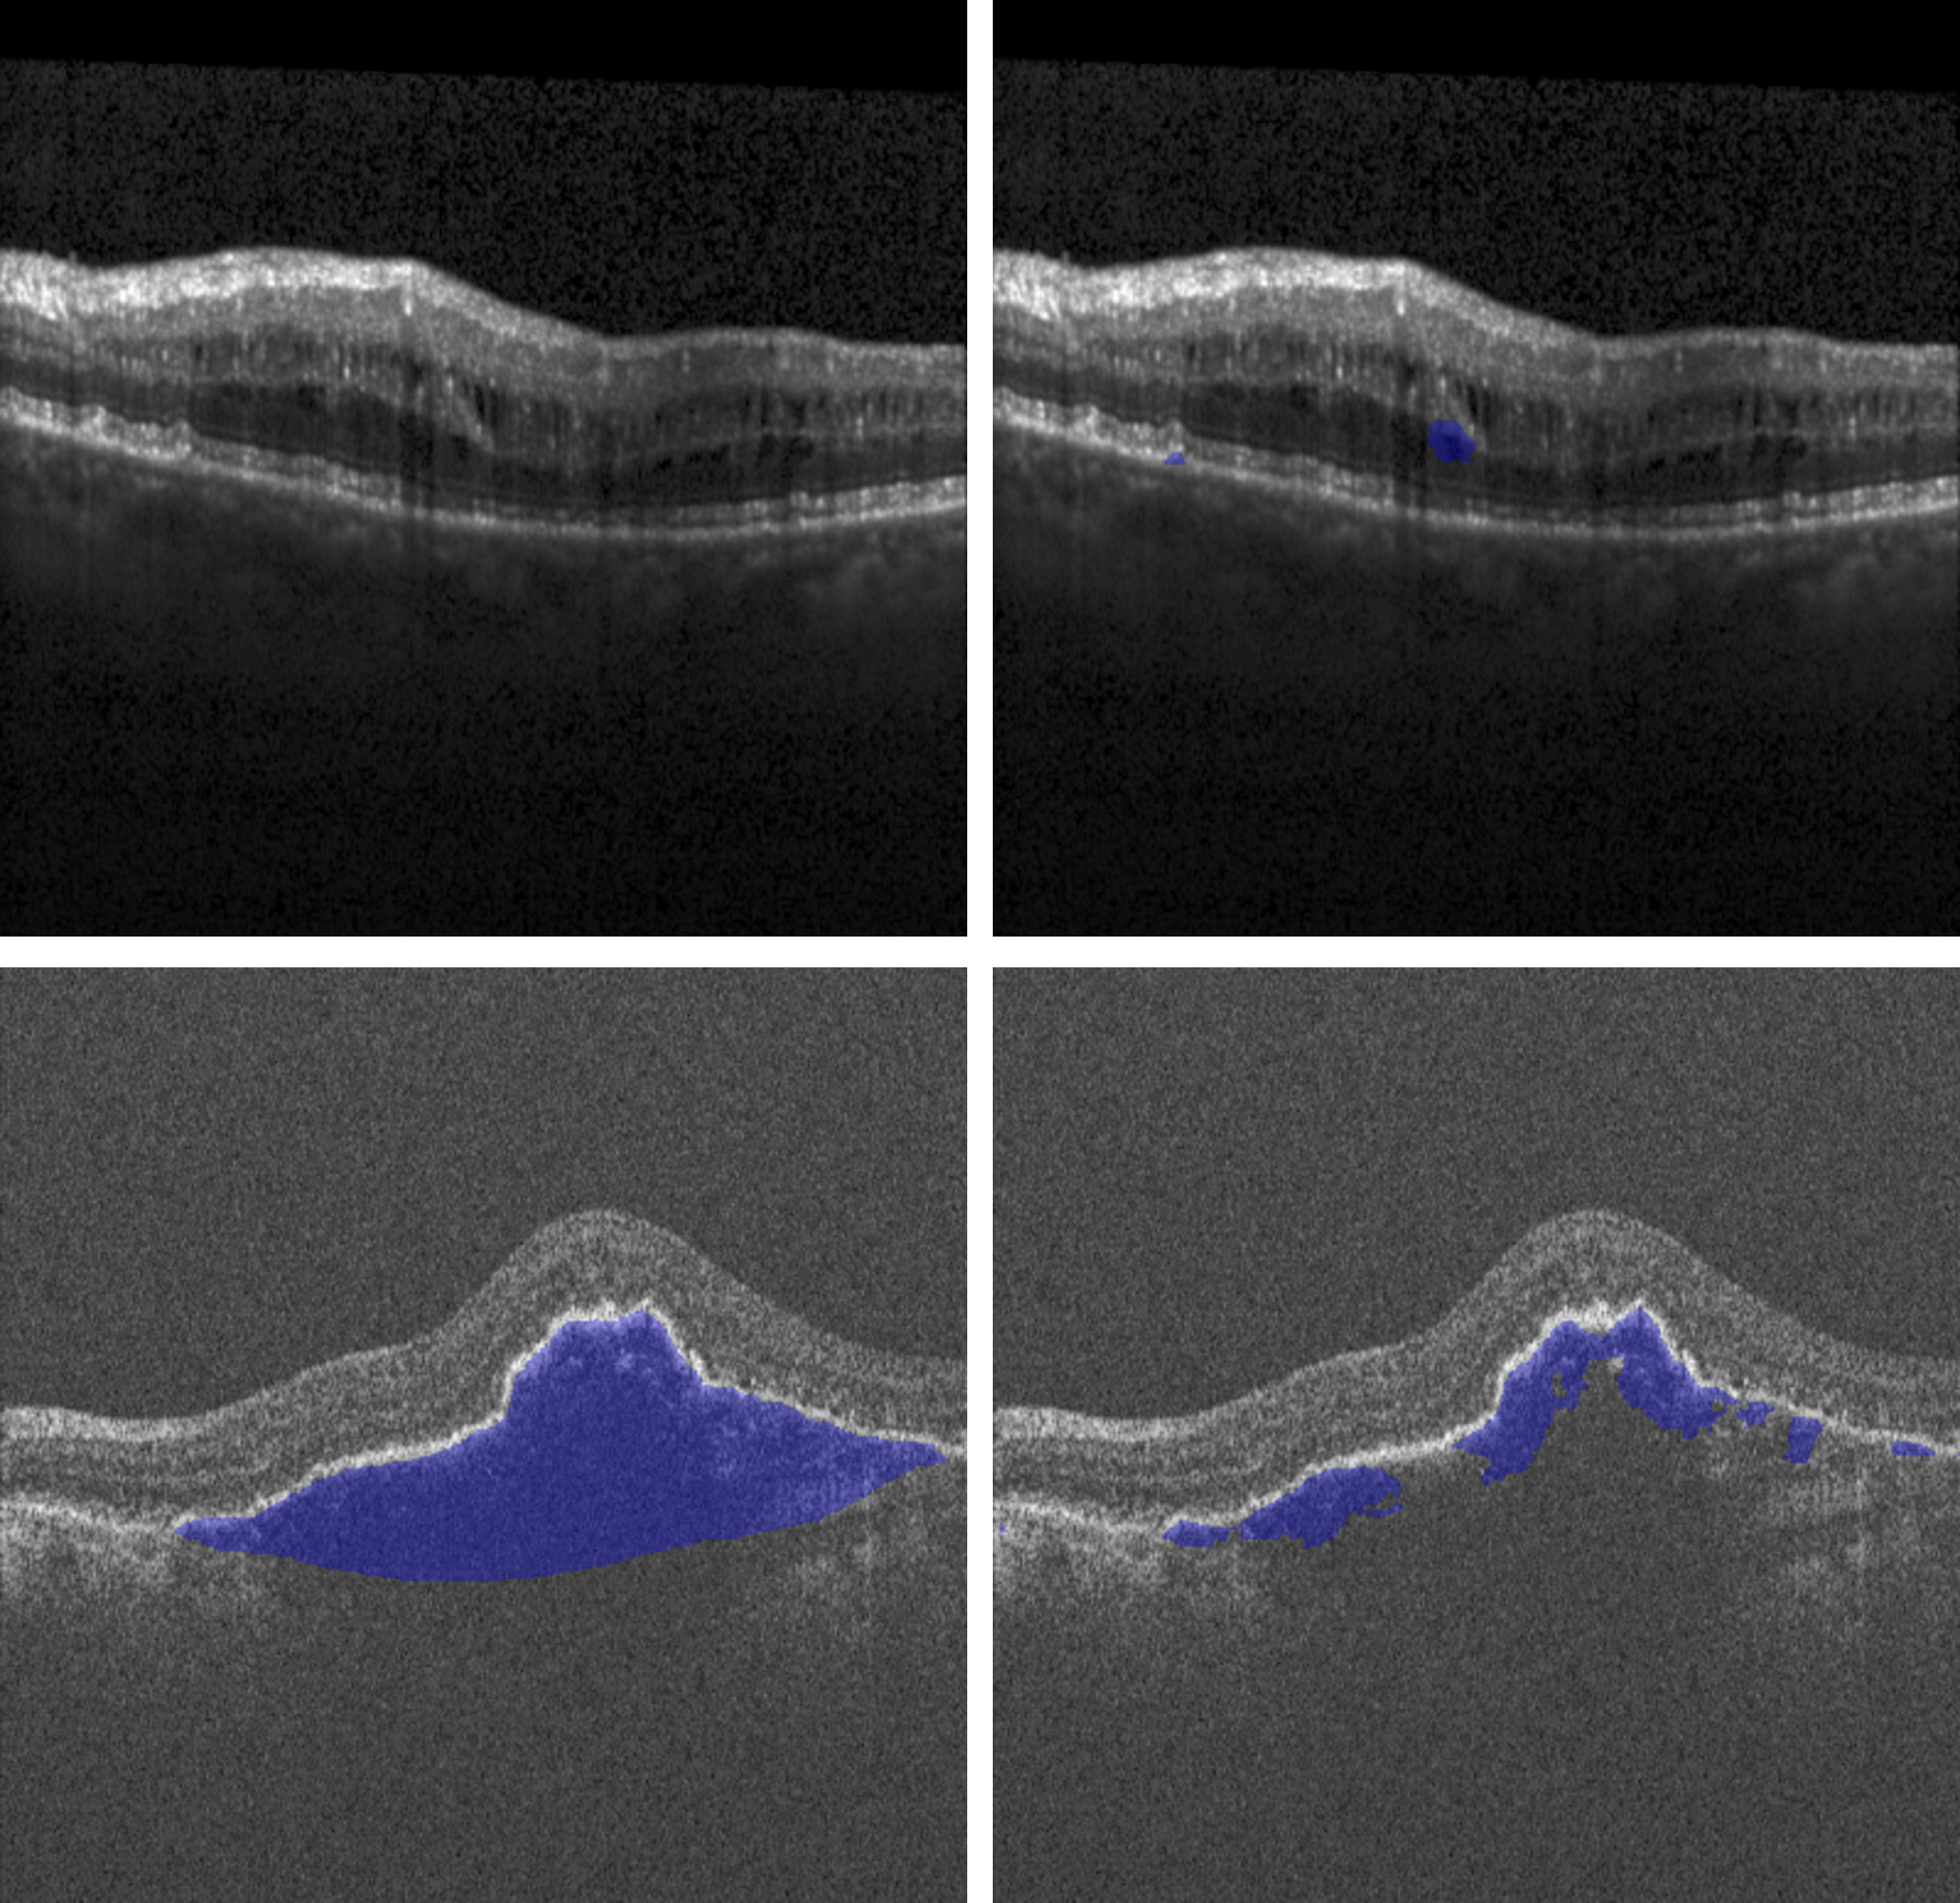
\includegraphics[width=0.7\linewidth]{figures/Experiment2PEDSegmentation.png}
	\caption{Predictions (right) performed by the binary PED segmentation model and their respective GT (left). In top right, the model predicted PED fluid in a region where it does not exist. The bottom images show the undersegmentation of the model trained in Run 59. While this model is capable of detecting the fluid location, it fails to segment its entirety.}
	\label{fig:Experiment2PEDSegmentation}
\end{figure}

In order to compare the results from this Experiment to the ones obtained in Experiment 1, three models had to be selected: one for IRF, one for SRF, and one for PED. Since the results obtained in Experiment 2.2 were much worse than the results reached in this experiment, the models selected for the inference in the unseen fold were selected from the runs performed in Experiment 2.1.
\par
From the models trained for IRF segmentation, ranging from Run 37 to Run 44, the model which obtained the best performance was the one trained on Run 42, as seen in Table \ref{tab:Experiment2IRF}. This model reached the best average performance in the segmentation of IRF both in all slices and when only slices with IRF were considered. In the other metrics, this model's performance were consistently similar to the best performing model in each metric. When compared to the average model from ``Set 7'', this model reached better performances in most metrics.
\par
The model selected to infer the SRF masks in the unseen fold was the model trained on Run 52. This model was the best performing SRF model in fluid segmentation in slices where SRF is present. In the other metrics, it performed closely to the best models, surpassing the average model from ``Set 7'' in most metrics.
\par
In PED, the selected model was the one trained on Run 59. This model was the best model in PED segmentation in slices that contain this fluid, with a significant difference from the other models. When considering all the slices, the model was the second best, but with a weak performance. Regarding the slices with fluid, this model outperformed the average from ``Set 7'' in all vendors. However, similar to all the other models trained for the binary segmentation of PED, it achieved a significantly worse performance when compared to the ones obtained in multi-class.
\par
When merging the masks from three independent binary segmentation models with the goal of outputting a multi-class segmentation, overlaps may occur, where multiple models assign different fluid labels to the same pixel. To resolve this conflict, two alternatives were explored in this fold: a priority-based approach, where the SRF takes precedence over IRF, which in turn takes precedence over PED; and a probability-based approach, where the predicted probabilities for the pixel are compared, attributing the label with highest predicted probability to it. An example of merging using probability-based approach compared to the priority based approach is seen in Figure .

\begin{figure}[!ht]
	\centering
	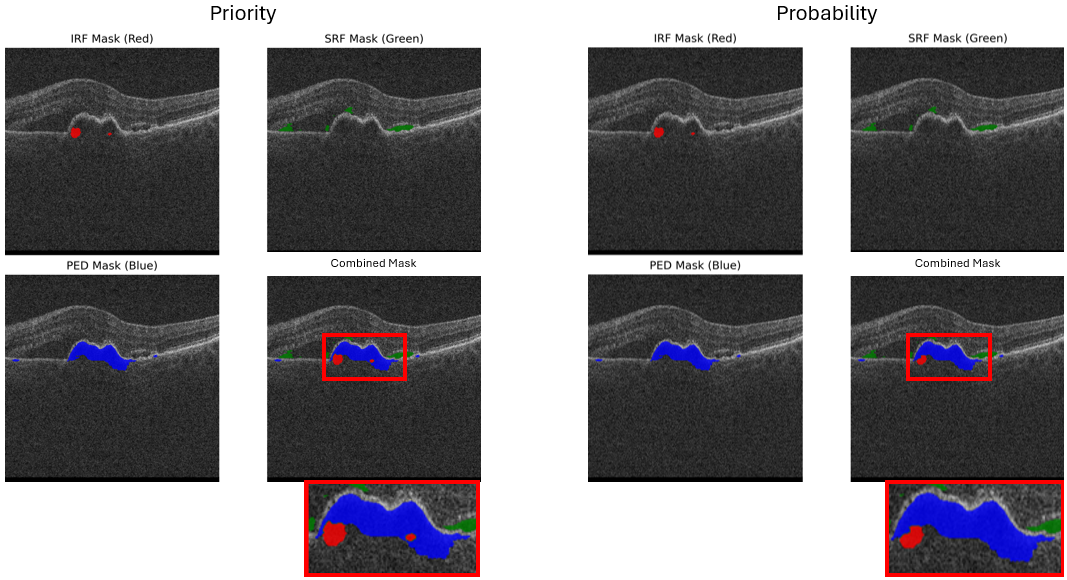
\includegraphics[width=1.0\linewidth]{figures/ProbabilityVsPrioritySegmentation.png}
	\caption{Comparison between the priority (left) and probability (right) merging approach.}
	\label{fig:ProbabilityVsPrioritySegmentation}
\end{figure}

The results obtained using the three selected models are shown in Table \ref{tab:Experiment2FinalResults}, where the first block corresponds to the results when using the priority-based merging approach and the second block presents the results when using the probability-based approach.

\begin{table*}[!ht]
	\caption{Dice scores for every vendor and fluid in the reserved fold (fold 1), using the models from Runs 42, for IRF, 52, for SRF, and 59, for PED. The first block corresponds to the results when using the priority rule merging strategy, while the second block is associated with the results when using highest probability as the merging strategy. In each block, the first row reports the mean Dice across all slices. The second row shows the mean for slices containing the fluid specified in the column, while the third shows the mean for the slices without that fluid. The values marked in bold are the best values when corresponding rows are compared, so that, for example, the row ``All'' in the first block is compared to the row of same name in the second.}
	\centering
	\resizebox{\textwidth}{!}{\begin{tabular}{|c|c|c|ccc|ccc|ccc|c|c|c|c|}
			\hline
			% Headers
			\multirow{2}{*}{\textbf{Runs}} &
			\multirow{2}{*}{\textbf{Slices}} &  
			\multirow{2}{*}{\textbf{VF}} & 
			\multicolumn{3}{c|}{\textbf{Cirrus}} & 
			\multicolumn{3}{c|}{\textbf{Spectralis}} & 
			\multicolumn{3}{c|}{\textbf{Topcon}} & 
			\multicolumn{1}{c|}{\multirow{2}{*}{\textbf{IRF}}} & 
			\multirow{2}{*}{\textbf{SRF}} & 
			\multirow{2}{*}{\textbf{PED}} & 
			\multirow{2}{*}{\textbf{Fluid}} \\ \cline{4-12} & & &
			\multicolumn{1}{c}{\textbf{IRF}} & 
			\multicolumn{1}{c}{\textbf{SRF}} & 
			\textbf{\textbf{PED}} & 
			\multicolumn{1}{c}{\textbf{IRF}} & 
			\multicolumn{1}{c}{\textbf{SRF}} & 
			\textbf{PED} & 
			\textbf{IRF} & 
			\textbf{SRF} & 
			\textbf{PED} & 
			\multicolumn{1}{c|}{} & & & \\ 
			
			\hline
			
			\multirow{3}{*}{\parbox{2cm}{\textbf{Runs 42, 52, and 59}}} & All & 1 & \multicolumn{1}{c|}{0.693} & \multicolumn{1}{c|}{0.776} & 0.425 & \multicolumn{1}{c|}{0.587} & \multicolumn{1}{c|}{0.623} & 0.177 & \multicolumn{1}{c|}{0.808} & \multicolumn{1}{c|}{0.858} & \textbf{0.531} & 0.723 & 0.783 & 0.425 & \textbf{0.544} \\
			
			& Fluid & 1 & \multicolumn{1}{c|}{0.687} & \multicolumn{1}{c|}{\textbf{0.670}} & 0.573 & \multicolumn{1}{c|}{\textbf{0.660}} & \multicolumn{1}{c|}{\textbf{0.659}} & 0.632 & \multicolumn{1}{c|}{\textbf{0.634}} & \multicolumn{1}{c|}{\textbf{0.560}} & \textbf{0.484} & \textbf{0.661} & \textbf{0.640} & 0.570 & \textbf{0.639} \\
			
			& No Fluid & 1 & \multicolumn{1}{c|}{0.695} & \multicolumn{1}{c|}{0.824} & \textbf{0.387} & \multicolumn{1}{c|}{\textbf{0.520}} & \multicolumn{1}{c|}{0.605} & \textbf{0.075} & \multicolumn{1}{c|}{0.867} & \multicolumn{1}{c|}{0.907} & \textbf{0.534} & 0.752 & 0.830 & \textbf{0.402} & \textbf{0.440} \\
			
			\hline
			\hline
			
			\multirow{3}{*}{\parbox{2cm}{\textbf{Runs 42, 52, and 59}}} & All & 1 & \multicolumn{1}{c|}{\textbf{0.697}} & \multicolumn{1}{c|}{\textbf{0.787}} & \textbf{0.428} & \multicolumn{1}{c|}{\textbf{0.628}} & \multicolumn{1}{c|}{\textbf{0.631}} & \textbf{0.178} & \multicolumn{1}{c|}{\textbf{0.810}} & \multicolumn{1}{c|}{\textbf{0.864}} & \textbf{0.531} & \textbf{0.733} & \textbf{0.792} & \textbf{0.427} & \textbf{0.544} \\
			
			& Fluid & 1 & \multicolumn{1}{c|}{\textbf{0.688}} & \multicolumn{1}{c|}{0.663} & \textbf{0.586} & \multicolumn{1}{c|}{\textbf{0.660}} & \multicolumn{1}{c|}{0.646} & \textbf{0.636} & \multicolumn{1}{c|}{0.632} & \multicolumn{1}{c|}{0.537} & \textbf{0.484} & \textbf{0.661} & 0.627 & \textbf{0.578} & \textbf{0.639} \\
			
			& No Fluid & 1 & \multicolumn{1}{c|}{\textbf{0.701}} & \multicolumn{1}{c|}{\textbf{0.844}} & \textbf{0.387} & \multicolumn{1}{c|}{\textbf{0.520}} & \multicolumn{1}{c|}{\textbf{0.623}} & \textbf{0.075} & \multicolumn{1}{c|}{\textbf{0.870}} & \multicolumn{1}{c|}{\textbf{0.917}} & \textbf{0.534} & \textbf{0.766} & \textbf{0.844} & \textbf{0.402} & \textbf{0.440} \\
			
			\hline
			
	\end{tabular}}
	\label{tab:Experiment2FinalResults}
\end{table*}

The performances of the models shown in this table, indicate that the best merging strategy is the probability-based. In the slices that contain the evaluated fluid, the priority-based approach performs better in SRF, since it is the fluid of highest priority. Regarding IRF, in the slices where this fluid is present, the performance is equal for both approaches, while in PED the probability-based approach is better.
\par
However, when considering all the slices, the approach based on the probability of each model is significantly better. This is tied to the better performance in the slices that do not contain at least on type of fluid. In these slices, this approach prevents the segmentation of the fluids which are not present in the slice. These oversegmentations can be wrongfully predicted in the region of other fluids. However, since the models responsible for correctly segmenting this region are more confident than the models that are wrongfully segmenting it, the labels are attributed to the correct class.
\par
It is important to note that the ``Fluid'' column does not change when using different merging approaches. This is because the region of fluid segmented stays the same, since the only changes performed are in pixels contested by multiple fluids, and if all the fluids belonged to a single class, as considered in this column, no changes would be made.
\par
The overall segmentation performance was comparable to the values obtained in the validation folds, during training. In IRF, the model trained in Run 42 reaches better results in this unseen fold than in the fold in which it was originally validated. This is true when considering all the slices, just those with IRF, or the slices without IRF, which signals the good generalization by the model.
\par
In the segmentation of SRF, the model did not perform as good in this fold. The fluid detection was better, seen by the significant increase in Dice coefficient when considering all the slices instead of just those with fluid, which opposes the results obtained in the validation in Run 52, where the performance decreases in this situation. However, the segmentation worsened significantly in the slices with SRF, as the Dice coefficient dropped from 0.819 in its original validation fold to 0.627. Nevertheless, when considering all the slices, the Dice coefficients are still similar, largely due to the improved Dice in the slices without SRF.
\par
When segmenting IRF and SRF, the models benefited from a good generalization in fluid detection task, which surpassed the performances originally obtained in validation. However, in PED, where the models were the most sensitive in this matter, the performance in this task was worse. It is the only fluid in which the Dice is worse when considering all the slices than when considering just the slices with the fluid. This performance is tied to the model selected for PED segmentation. As seen in Table \ref{tab:Experiment2PED}, the model trained in Run 59 already presents a subpar performance in fluid detection, seen by the decrease in Dice coefficient when considering all the slices instead of those that contain PED. Therefore, the poor detection in unseen images is not unexpected. Note that the model selected detects fluid worse in the Spectralis volumes, similar to what was seen in the model validation. Similarly, the vendor in which the best performance is attained is the Topcon, where the model also performed best during validation. Moreover, all the PED models were expected to generalize worse in the unseen fold in the fluid detection task, due to the reasons previously presented that justify the lack of robustness in these models, such as the heterogeneous distribution of PED in OCT volumes.
\par
In Figures \ref{fig:Experiment2FinalModelPredictionsCirrus}, \ref{fig:Experiment2FinalModelPredictionsSpectralis}, and \ref{fig:Experiment2FinalModelPredictionsTopcon}, it is possible to see the predictions made by the multi-class segmentation performed by binary models specific for each fluid, in Cirrus, Spectralis, and Topcon, respectively. The B-scans presented in these figures are the same as those shown in Experiment 1. In the first row, the GT of each B-scans segmentation is shown, while in the second row the segmentations were performed by the best multi-class model selected in Experiment 1. In the last row, the predictions made by the best models from Experiment 2 are shown.

\begin{figure}[!ht]
	\centering
	\includegraphics[width=0.7\linewidth]{figures/Experiment2FinalModelPredictionsCirrus.png}
	\caption{Predictions by the models trained on Run 42, 52, and 59 in unseen Cirrus volumes of fold 1 (last row), contrasting with predictions made by the multi-class model from Experiment 1.}
	\label{fig:Experiment2FinalModelPredictionsCirrus}
\end{figure}

\begin{figure}[!ht]
	\centering
	\includegraphics[width=0.7\linewidth]{figures/Experiment2FinalModelPredictionsSpectralis.png}
	\caption{Predictions by the models trained on Run 42, 52, and 59 in unseen Spectralis volumes of fold 1 (last row), contrasting with predictions made by the multi-class model from Experiment 1.}
	\label{fig:Experiment2FinalModelPredictionsSpectralis}
\end{figure}

\begin{figure}[!ht]
	\centering
	\includegraphics[width=0.7\linewidth]{figures/Experiment2FinalModelPredictionsTopcon.png}
	\caption{Predictions by the models trained on Run 42, 52, and 59 in unseen Topcon volumes of fold 1 (last row), contrasting with predictions made by the multi-class model from Experiment 1.}
	\label{fig:Experiment2FinalModelPredictionsTopcon}
\end{figure}

\subsubsection{Experiment 2.2}

In this experiment, the loss function used in the training of the segmentation models was changed from a combination of a weighted cross-entropy and Dice coefficient of the foreground to the weighted cross-entropy. The results are shown in Table \ref{tab:Experiment2.2Results}, where only two runs were performed for the segmentation of IRF, one in each 5-fold split. 

\begin{table*}[!ht]
	\caption{IRF Dice scores for every vendor, using the binary segmentation U-Net for IRF. The loss function used in Runs 61 and 62 is the weighted cross-entropy. This model was trained on two different validation folds: validation fold 0 from the multi-class 5-fold split, and validation fold 4 from the 5-fold split specific for IRF. These results can be compared, respectively, to those obtained in Runs 40 and 43. The metrics are compared between rows with the same name, so that the values in bold are the best across the four experiments.}
	\centering
	\begin{tabular}{|c|c|c|c|c|c|c|}
			\hline
			% Headers
			\textbf{Runs} &
			\textbf{Slices} &  
			\textbf{VF} & 
			\textbf{Cirrus} & 
			\textbf{Spectralis} & 
			\textbf{Topcon} & 
			\textbf{IRF} \\ 
			
			\hline
			
			\multirow{3}{*}{\textbf{Run 61}} & All & 0 & 0.088 & 0.164 & 0.121 & 0.113 \\
			
			& Fluid & 0 & 0.320 & 0.390 & 0.472 & 0.378 \\
			
			& No Fluid & 0 & 0.002 & 0.044 & 0.041 & 0.024 \\
			
			\hline
			
			\multirow{3}{*}{\textbf{Run 62}} & All & 4 & 0.130 & 0.250 & 0.142 & 0.151 \\
			
			& Fluid & 4 & 0.399 & 0.531 & 0.549 & 0.466 \\
						
			& No Fluid & 4 & 0.000 & 0.052 & 0.053 & 0.030 \\
			
			\hline
			\hline
			
			\multirow{3}{*}{\textbf{Run 40}} & All & 0 & 0.576 & \textbf{0.695} & \textbf{0.661} & \textbf{0.628} \\
			
			& Fluid & 0 & \textbf{0.619} & \textbf{0.682} & \textbf{0.599} & \textbf{0.628} \\
			
			& No Fluid & 0 & 0.555 & 0.705 & \textbf{0.686} & \textbf{0.628} \\
			
			\hline
			
			\multirow{3}{*}{\textbf{Run 43}} & All & 4 & \textbf{0.583} & 0.689 & 0.310 & 0.502 \\
			
			& Fluid & 4 & 0.516 & 0.660 & 0.451 & 0.546 \\
			
			& No Fluid & 4 & \textbf{0.601} & \textbf{0.719} & 0.272 & 0.486 \\
			
			\hline
			
	\end{tabular}
	\label{tab:Experiment2.2Results}
\end{table*}

The results seen in the table are much worse than those obtained in the same conditions with the previous loss. In the slices with IRF, the segmentation was poor, but with a performance almost comparable to the values obtained in Run 40 and 43.
\par
However, what really worsens the overall performance is fluid detection. All the Dice coefficients in the slices with no fluid were inferior than 0.05, while most of the models studied in Experiment 2.1 reached values superior than 0.5.
\par
The reason these values were so low is related with the loss function used. By keeping the Dice loss as a component of the training loss, the model is highly penalized when predicting fluid in an image which does not have fluid. Whenever any fluid is predicted in such image, the Dice coefficient is 0. This motivates the model to carefully predict pixels in regions of the image where it highly believes there is fluid.
\par
When removing the Dice component from the loss, the wrongful predictions are only penalized by the cross-entropy component. This component does not penalize as much the predictions of fluid in empty images. The cross-entropy of each B-scan is calculated adjusted to the number of pixels belonging to a class in the image, as shown in \ref{Methods} Methods. Whenever a background pixel is wrongfully classified as fluid, the resulting penalty is really small, due to the large quantity of background pixels in the mask. Therefore, the motivation to not segment fluid in images which are solely composed of background is much smaller than it is when the Dice is considered. This results in segmentations such as the one seen in Figure \ref{fig:BCESegmentationError}.
\par
The cross-entropy is much more useful when regularizing the wrong labeling, especially in fluid. Since this loss component is adjusted to the representation of each class in the image, wrongfully labeling a fluid region as another fluid or background brings a large penalty to the model. This is why it is combined with the Dice loss in the original loss: while the Dice ensures that the correct areas of fluid are segmented, the cross-entropy makes sure that the correct labels are assigned to each pixel. For this reason, most of the segmentation errors that are seen in the predictions made by the models trained in Run 61 and 62 are oversegmentations, and not as many incorrect labelings. An example of how this translates to the model's segmentation is seen in Figure \ref{fig:BCESegmentationDecent}.

\begin{figure}[!ht]
	\centering
	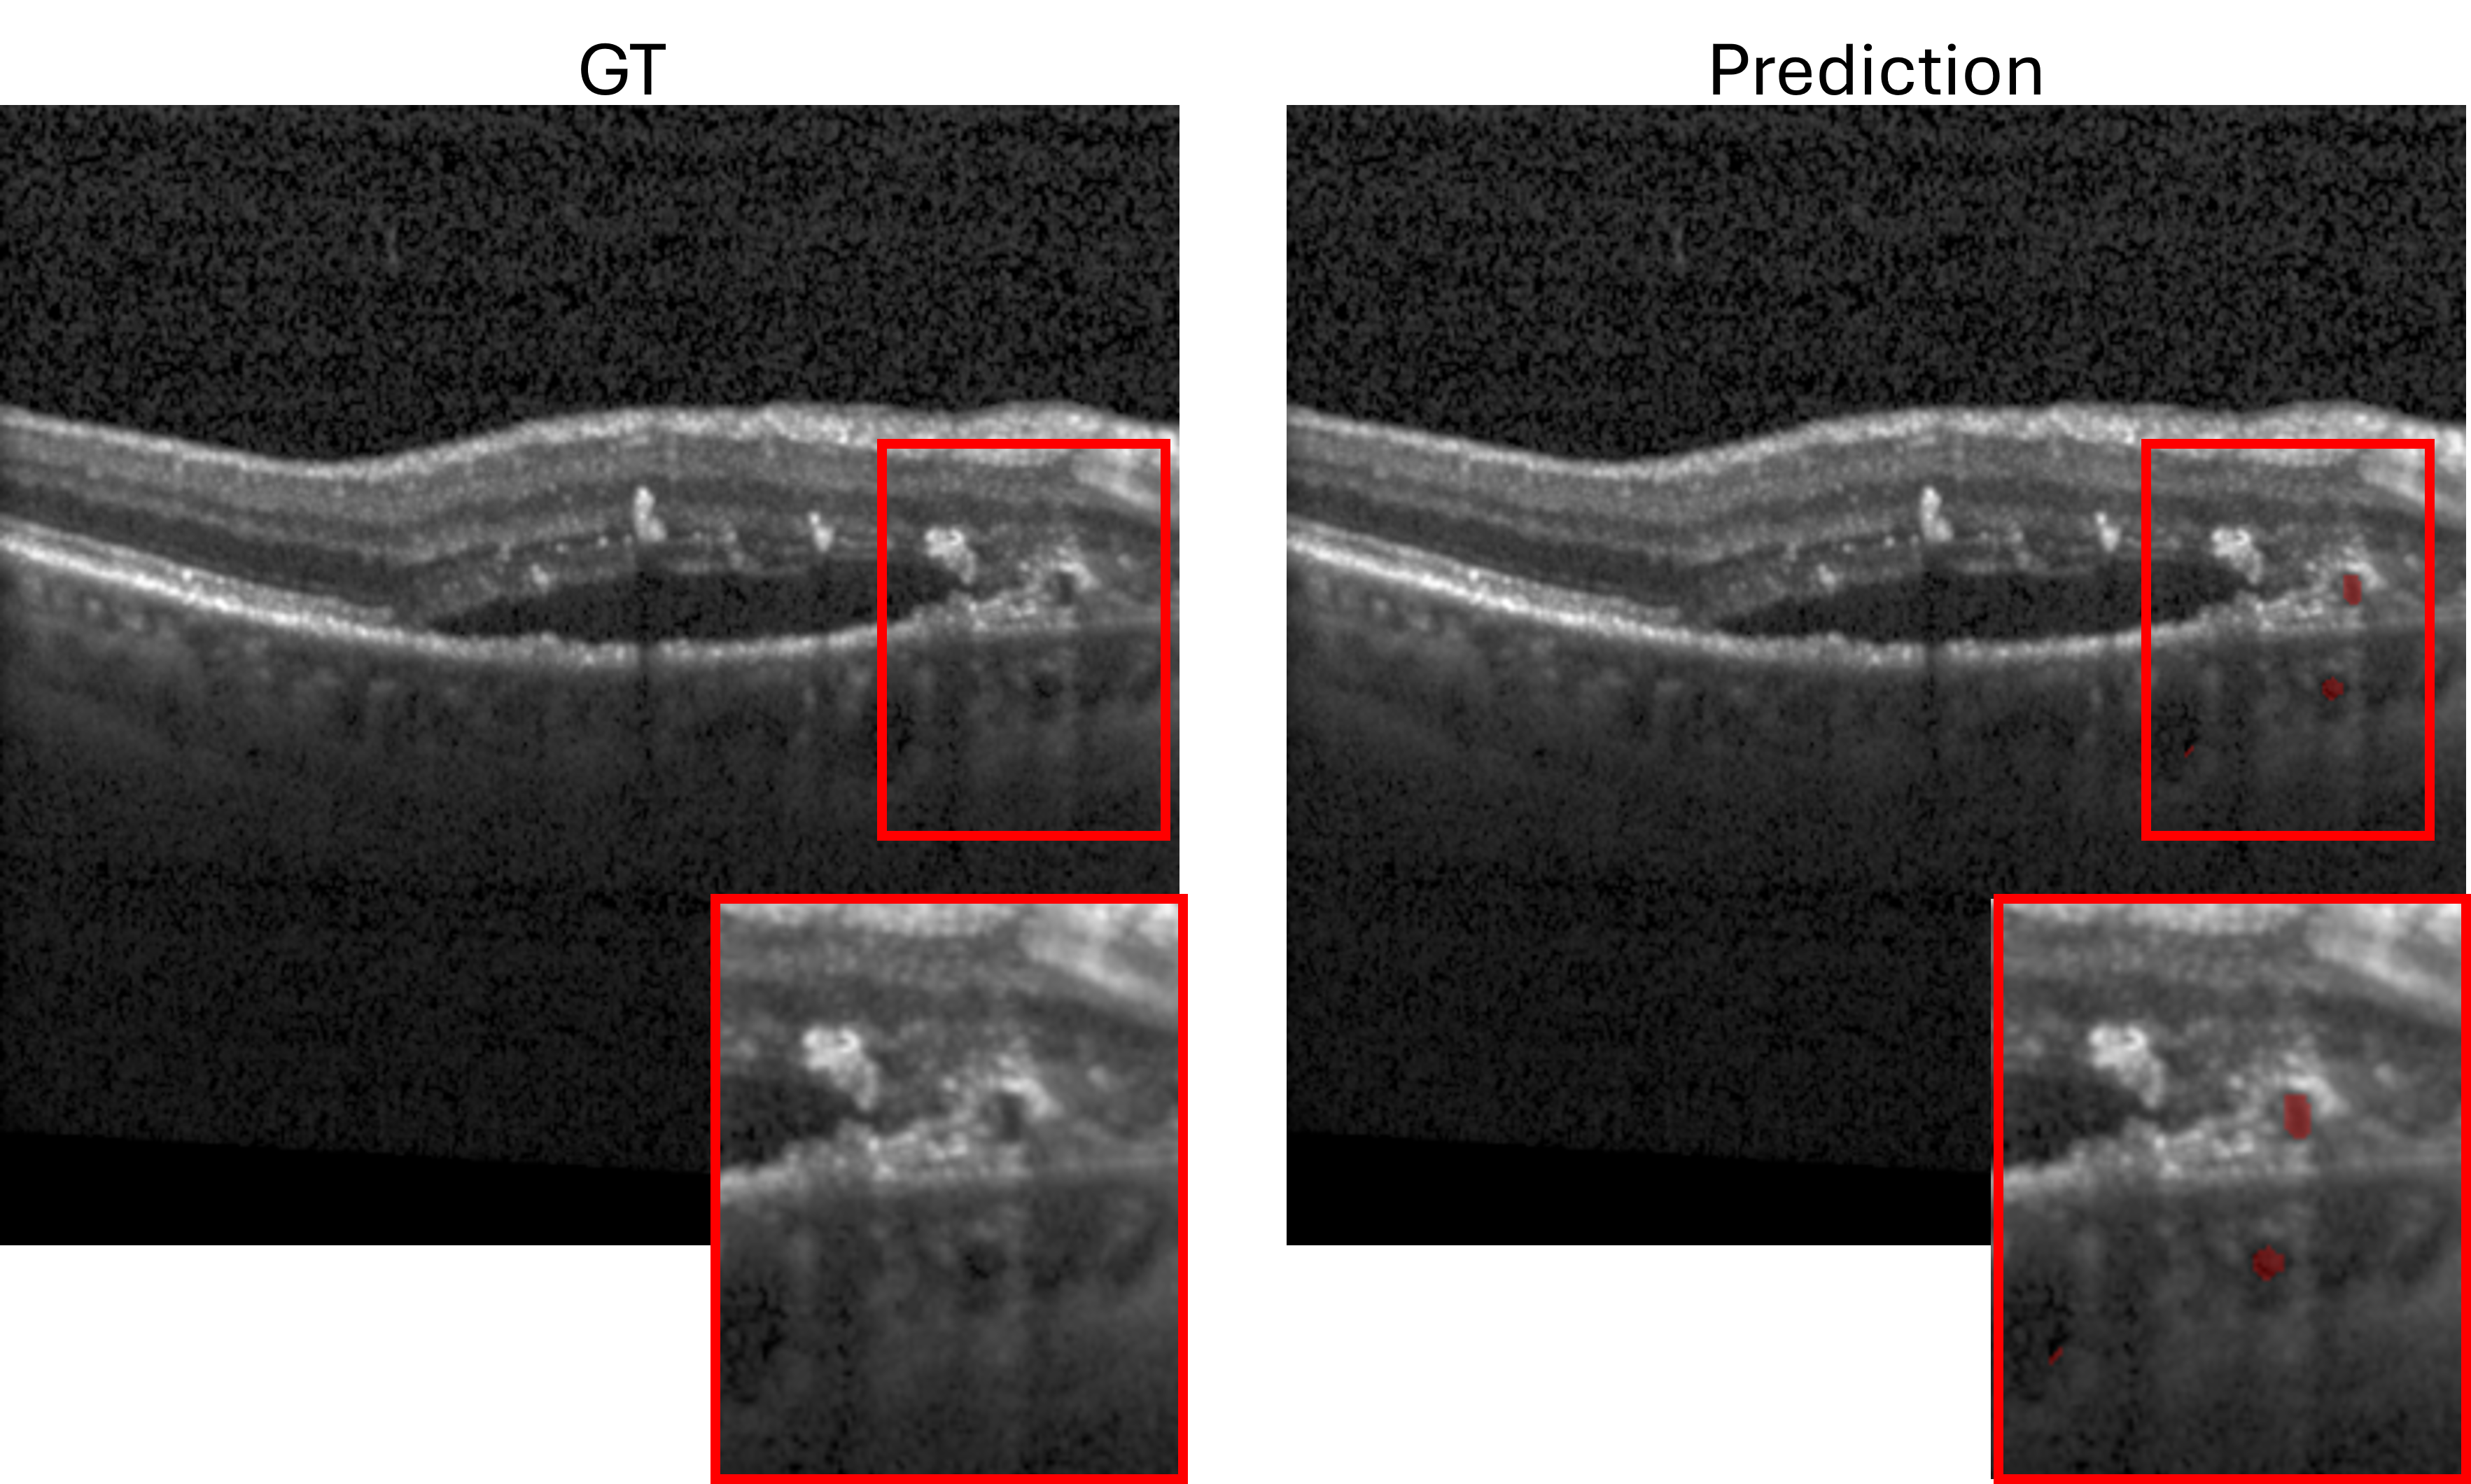
\includegraphics[width=0.8\linewidth]{figures/BCESegmentationError.png}
	\caption{Small oversegmentation performed in a Spectralis B-scan. This type of predictions appear commonly across multiple B-scans.}
	\label{fig:BCESegmentationError}
\end{figure}

\begin{figure}[!ht]
	\centering
	\includegraphics[width=0.8\linewidth]{figures/BCESegmentationDecent.png}
	\caption{Cirrus IRF segmentation performed by a model trained using BCE shown on the right, compared to its GT on the left. While this example has a decent segmentation, significant oversegmentation is seen on the top left of the image.}
	\label{fig:BCESegmentationDecent}
\end{figure}

\subsection{Experiment 1 and Experiment 2 Comparison in RETOUCH Dataset}

In order to compare Experiment 1 with Experiment 2, both their performances were presented in Table \ref{tab:Experiment1VsExperiment2}. These experiments are compared by evaluating each experiment's performance on the reserved fold. In the table, the first block corresponds to the performance obtained with the selected multi-class segmentation model, while the second block shows the performance of the combination of models from Experiment 2, with their masks combined in a probability-based approach.

\begin{table*}[!ht]
	\caption{Dice scores for every vendor and fluid in the reserved fold (fold 1), using the best models from Experiment 1 and Experiment 2. In Experiment 1, the model trained on Run 32 was selected, while in Experiment 2 the chosen models were those from Runs 42, for IRF, 52, for SRF, and 59, for PED. The rows with the same name must be compared with each other.}
	\centering
	\resizebox{\textwidth}{!}{\begin{tabular}{|c|c|c|ccc|ccc|ccc|c|c|c|c|}
			\hline
			% Headers
			\multirow{2}{*}{\textbf{Runs}} &
			\multirow{2}{*}{\textbf{Slices}} &  
			\multirow{2}{*}{\textbf{VF}} & 
			\multicolumn{3}{c|}{\textbf{Cirrus}} & 
			\multicolumn{3}{c|}{\textbf{Spectralis}} & 
			\multicolumn{3}{c|}{\textbf{Topcon}} & 
			\multicolumn{1}{c|}{\multirow{2}{*}{\textbf{IRF}}} & 
			\multirow{2}{*}{\textbf{SRF}} & 
			\multirow{2}{*}{\textbf{PED}} & 
			\multirow{2}{*}{\textbf{Fluid}} \\ \cline{4-12} & & &
			\multicolumn{1}{c}{\textbf{IRF}} & 
			\multicolumn{1}{c}{\textbf{SRF}} & 
			\textbf{\textbf{PED}} & 
			\multicolumn{1}{c}{\textbf{IRF}} & 
			\multicolumn{1}{c}{\textbf{SRF}} & 
			\textbf{PED} & 
			\textbf{IRF} & 
			\textbf{SRF} & 
			\textbf{PED} & 
			\multicolumn{1}{c|}{} & & & \\ 
			
			\hline

			\multirow{3}{*}{\textbf{Run 32}} & All & 1 & \multicolumn{1}{c|}{\textbf{0.852}} & \multicolumn{1}{c|}{\textbf{0.918}} & \textbf{0.934} & \multicolumn{1}{c|}{\textbf{0.645}} & \multicolumn{1}{c|}{\textbf{0.821}} & \textbf{0.852} & \multicolumn{1}{c|}{\textbf{0.818}} & \multicolumn{1}{c|}{\textbf{0.929}} & \textbf{0.755} & \textbf{0.799} & \textbf{0.905} & \textbf{0.841} & \textbf{0.742} \\
			
			& Fluid & 1 & \multicolumn{1}{c|}{0.654} & \multicolumn{1}{c|}{\textbf{0.799}} & \textbf{0.767} & \multicolumn{1}{c|}{0.645} & \multicolumn{1}{c|}{\textbf{0.687}} & \textbf{0.703} & \multicolumn{1}{c|}{0.624} & \multicolumn{1}{c|}{\textbf{0.744}} & \textbf{0.588} & 0.641 & \textbf{0.756} & \textbf{0.716} & \textbf{0.702} \\
			
			& No Fluid & 1 & \multicolumn{1}{c|}{\textbf{0.941}} & \multicolumn{1}{c|}{\textbf{0.972}} & \textbf{0.978} & \multicolumn{1}{c|}{\textbf{0.646}} & \multicolumn{1}{c|}{\textbf{0.889}} & \textbf{0.885} & \multicolumn{1}{c|}{\textbf{0.884}} & \multicolumn{1}{c|}{\textbf{0.960}} & \textbf{0.766} & \textbf{0.873} & \textbf{0.952} & \textbf{0.862} & \textbf{0.786} \\
			
			\hline
			\hline
			
			\multirow{3}{*}{\parbox{2cm}{\textbf{Runs 42, 52, and 59}}} & All & 1 & \multicolumn{1}{c|}{0.697} & \multicolumn{1}{c|}{0.787} & 0.428 & \multicolumn{1}{c|}{0.628} & \multicolumn{1}{c|}{0.631} & 0.178 & \multicolumn{1}{c|}{0.810} & \multicolumn{1}{c|}{0.864} & 0.531 & 0.733 & 0.792 & 0.427 & 0.544 \\
			
			& Fluid & 1 & \multicolumn{1}{c|}{\textbf{0.688}} & \multicolumn{1}{c|}{0.663} & 0.586 & \multicolumn{1}{c|}{\textbf{0.660}} & \multicolumn{1}{c|}{0.646} & 0.636 & \multicolumn{1}{c|}{\textbf{0.632}} & \multicolumn{1}{c|}{0.537} & 0.484 & \textbf{0.661} & 0.627 & 0.578 & 0.639 \\
			
			& No Fluid & 1 & \multicolumn{1}{c|}{0.701} & \multicolumn{1}{c|}{0.844} & 0.387 & \multicolumn{1}{c|}{0.520} & \multicolumn{1}{c|}{0.623} & 0.075 & \multicolumn{1}{c|}{0.870} & \multicolumn{1}{c|}{0.917} & 0.534 & 0.766 & 0.844 & 0.402 & 0.440 \\
			
			\hline
			
	\end{tabular}}
	\label{tab:Experiment1VsExperiment2}
\end{table*}

By looking at this table, the best segmentation performance becomes evident. The multi-class model consistently outperforms the binary models in across all fluids, vendors, and slice groups.
\par
Regarding the performances in fluids, the multi-class segmentation performs better than the binary models in all fluids when all the slices are considered and when only the slices which do not contain a certain fluid are considered. The only metrics in which the binary models outperform the multi-class is the segmentation of IRF in slices which contain this fluid. In these metrics, the binary models attain small improvements over the multi-class model. This fluid was also the one with the best performance in the set of slices with IRF, in Experiment 2.1. However, the segmentation of IRF in the slices which contain this fluid is not enough to compensate for the worse performance in fluid detection, when considering the slices without IRF. This was seen the major flaw of the binary segmentation models, which is tied to the models' weaker capability of understanding anatomical structures. This leads to a worse overall performance in IRF even when the segmentation is better. An example of similar performances between these models is seen in the IRF segmentations of Figures \ref{fig:Experiment2FinalModelPredictionsCirrus}, \ref{fig:Experiment2FinalModelPredictionsSpectralis}, and \ref{fig:Experiment2FinalModelPredictionsTopcon}.
\par
The performances reached by the binary model in SRF are worse than those obtained with the multi-class. While the predictions made with the binary model are still satisfactory, they are not as good as those made by the multi-class, as seen in the first case of the Figures \ref{fig:Experiment2FinalModelPredictionsCirrus} and \ref{fig:Experiment2FinalModelPredictionsTopcon}. This model shows a great detection of fluid, with a Dice coefficient greater than 0.85 in all classes, and the best fluid segmentation of all classes.
\par
The biggest performance difference between models are those observed in the PED class. The segmentation of PED in slices which contain this fluid is worse in the binary model than in multi-class. Despite the segmentation being worse across all vendors, the performance in the binary model is still acceptable. However, in the detection of fluid, the binary model performs poorly, especially when compared to the multi-class. These results are tied to the models' capabilities in identifying the region in which PED is located, which was seen to be much superior in multi-class. Two examples which show this are seen in the left side of Figure \ref{fig:Experiment2FinalModelPredictionsCirrus} and the segmentation in the bottom of Figure \ref{fig:Experiment2PEDSegmentation}, where the region segmented by PED does not occupy the entirety of the fluid, but only the section closest to its upper boundary.
\par
It is important to compare the results in the RETOUCH dataset with those obtained in the literature to better understand the impact and effect of the chosen methodology. \textcite{Alsaih2020} present an insightful study on the performance of multiple networks, including the U-Net, in the RETOUCH dataset. This paper was chosen as a benchmark for comparison due to the used dataset and the similarity with the selected methods. 
\par
In this article, the networks were trained and evaluated following a 3-fold approach, with the OCT volumes being equally distributed across the folds while still keeping a fair representation of vendors. The implementations in Experiment 1 and Experiment 2 were compared to two other base U-Net implementations in this paper: one trained with the entire image and another trained with patches. Multiple patch shapes (32 $\times$ 32, 64 $\times$ 64, 96 $\times$ 96, 128 $\times$ 128, 256 $\times$ 256, and 512 $\times$ 512) extracted with different overlapping percentages were tested, but the selected was 128 $\times$ 128 with 80\% overlapping as they obtained the best results. All the B-scans were previously resized to 572 $\times$ 572.
\par
For each model, \textcite{Alsaih2020} trained three networks with different optimizers: one using the stochastic gradient descent while the other two were trained using the Adam. Then, the results from each network were fused through majority voting. The results were also post-processed using a median filter.
\par
These differences bring advantages to the implementations by \textcite{Alsaih2020}, as they enhance the robustness and overall segmentation performance. While these changes provide a performance edge, it is challenging to find other studies with a comparable setup in terms of network architecture, dataset, and evaluation protocol. For these reasons, this paper was considered the most similar and, overall, suitable for comparison with the experiments presented here.
\par
In Table \ref{tab:Experiment1VsExperiment2VsLiterature}, the mean of the results in three validation folds of the models trained in \textcite{Alsaih2020} are shown, as well as the results from ``Set 7'' and ``Sets 10, 12, and 14'' together, representing the multiple binary models used in Experiment 2.

\begin{table*}[!ht]
	\caption{Dice scores for every fluid in ``Set 7'', ``Set 10, 12, and 14'', compared with the results obtained in the two networks by \textcite{Alsaih2020}.}
	\centering
	\begin{tabular}{|c|c|c|c|}
			\hline
			% Headers
			\textbf{Runs} & \textbf{IRF} & 
			\textbf{SRF} & 
			\textbf{PED} \\
						
			\hline
			
			\textbf{Set 7} & 0.67 & \textbf{0.80} & 0.72 \\
			
			\hline
			
			\textbf{Sets 10, 12, and 14} & 0.60 & 0.75 & 0.44 \\
			
			\hline
			\hline
			
			\textbf{U-Net \parencite{Alsaih2020}} & 0.29 & 0.47 & 0.18 \\
			
			\hline
			
			\textbf{U-Net with Patches \parencite{Alsaih2020}} & \textbf{0.68} & 0.61 & \textbf{0.84} \\
			
			\hline
			
	\end{tabular}
	\label{tab:Experiment1VsExperiment2VsLiterature}
\end{table*}

In this table, the first difference which presents a clear advantage in fluid segmentation is the use of patches as input. It becomes clear that the best segmentation performances in all fluids were achieved in the models which used patches. This enhances the model's capability of perceiving the image's finer details, which is deemed particularly helpful in IRF and PED.
\par
Despite the significant performance differences between the U-Net trained with the full image and the U-Net trained with patches implemented by \textcite{Alsaih2020}, the variation of performance in SRF is smaller than that seen in IRF and PED. This is because the use of patch-based inputs particularly favors the segmentation of localized fluids like IRF and PED, but not so much the SRF, since it depends on model capability to capture broader anatomical context. Since the SRF is often visually similar to the background, the patch-based approaches are more prone to misclassify it.
\par 
The use of vertical patches in Experiment 1 and 2 provides the anatomical context necessary for the segmentation of SRF, as reflected in the significantly better performance to that reported by \textcite{Alsaih2020}. In IRF segmentation, the difference in Dice scores between the two approaches is less pronounced. While the smaller patches used by \textcite{Alsaih2020} allow the model to focus on finer details, such as pixel intensity in fluid regions, the vertical patches from Experiment 1 and 2 offer a broader field of view that captures the structural references helpful for segmentation.
\par
For PED, the difference between experiments is also significant, though smaller than in SRF. However, the trend seen in this fluid is reversed to the one in SRF, as the models trained on smaller patches tend to perform better for PED. While models trained with vertical patches are more effective at determining the boundaries of PED fluid, they often lack the attention to the finer details. This is particularly relevant in cases with large PED regions, where the significant deformation of the retina causes parts of the fluid being positioned further away from key anatomical landmarks like the retinal layers. In such scenarios, models trained on smaller patches, which are attentive to details such as pixel intensity and less dependent on anatomical context, perform better. This contributes to the overall improved performance of models trained with smaller patches in segmenting PED.
\par
Overall, the models trained in Experiments 1 and 2 perform comparably or better than the U-Nets implemented by \textcite{Alsaih2020}, despite relying on a single network per task (one for multi-class segmentation in ``Set 7'' and one for binary segmentation in ``Sets 10, 12, and 14'') and excluding any post-processing steps. This highlights the effectiveness of the patch shape explored in these experiments, where it is both capable of capturing details fine enough to segment IRF, but also large enough to detect SRF. The absence of ensemble networks used for the same task or refinement techniques further emphasizes the robustness of the proposed approach, making it competitive and more efficient alternative for multi-class fluid segmentation in retinal OCT images.
\par
In a previous work, the authors also implemented the network developed by \textcite{Tennakoon2018}, using the same dataset. This network is a 2.5D segmentation network which receives three consecutive B-scans and segments the intermediate one. This model was trained in patches of shape 256 $\times$ 128, as done in Experiment 1.1 and the results from this model are shown in Table \ref{tab:Experiment1VsExperiment2VsTennakoon}. The implementation exhibited in this table corresponds to a single model performance, which was trained for 100 epochs using a 80\% training and 20\% testing split. A fair vendor representation was ensured in the split, but the quantities of fluid were not considered.

\begin{table*}[!ht]
	\caption{Dice scores for every vendor and fluid in Set 7, Set 10, 12, and 14, compared with the results obtained in the authors' previous implementation of the work by \textcite{Tennakoon2018}.}
	\centering
	\begin{tabular}{|c|c|c|c|c|}
		\hline
		% Headers
		\textbf{Runs} & \textbf{IRF} & 
		\textbf{SRF} & 
		\textbf{PED} &
		\textbf{Fluid} \\
		
		\hline
		
		\textbf{Set 7} & 0.67 & 0.80 & \textbf{0.72} & \textbf{0.63} \\
		
		\hline
		
		\textbf{Sets 10, 12, and 14} & 0.60 & 0.75 & 0.44 & - \\
		
		\hline
		\hline
		
		\textbf{\textcite{Tennakoon2018} Implementation} & \textbf{0.71} & \textbf{0.85} & 0.71 & 0.62 \\
		
		\hline
		
	\end{tabular}
	\label{tab:Experiment1VsExperiment2VsTennakoon}
\end{table*}

In this table, it is seen that the 2.5D implementation performs better than the models in ``Set 7'' and ``Sets 10, 12, and 14'' in IRF and SRF, but worse in PED and in overall fluid.
\par
The main advantage when using this model is the use of the surrounding slices as a way to capture the context around the fluid regions. The small transitions, which are noticeable when seeing three consecutive slices, allow the model to learn the limiting regions of the fluids. This understanding of surrounding areas, combined with the attention to small changes motivated by the training in small patches, makes this model capable of both fine and coarse segmentation, as it is able to know the limits of fluid regions independently of their size. 
\par
This explains the improved segmentation of SRF, as the model better captures the small transitions in the SRF regions while still understanding the changes in the space around it which allow for the identification of this fluid. Similarly, the small patches also promote a better segmentation of IRF, where the understanding of small transitions is required for a correct segmentation.
\par
In PED, the performance is worse, but mainly due to the conditions in which this model was trained. Since the data was split randomly, the training volumes contained large quantities of PED, which led to the prediction of significant quantities of this fluid in multiple B-scans. For this reason, the Dice coefficient when considering all the fluid as binary was also deeply penalized, as seen in the table. 
\par
However, it is important to note that the results shown do not come from a cross-validation, and instead of a single split. This means that not only the 2.5D segmentation model was trained on more data than the those in Experiment 1 and 2 (approximately 60\% of the RETOUCH dataset), it could also have a split which benefits or harms the models performance.

\subsection{Experiment 1 and Experiment 2 Comparison in CHUSJ Dataset}

The results obtained in the CHUSJ private dataset were not as good as those obtained in the \hbox{RETOUCH}, in which the model was trained. The main cause for this poor segmentation is difference between the RETOUCH and CHUSJ dataset regarding image quality and segmentation criteria. In Table \ref{tab:CHUSJSegmentationResults}, the Dice coefficients across multiple vendors and fluids are shown, both for the images in their original shape and resized to $496 \times 512$. Since the segmentation U-Net is a fully convolutional network and does not contain any shape-dependent layer, the trained models can be applied to dataset B-scans in their original shape or resized.

\begin{table*}[!ht]
	\caption{Dice scores for every vendor and fluid in the CHUSJ dataset, using the best models from Experiment 1 and Experiment 2.}
	\centering
	\begin{tabular}{|c|c|c|c|c|c|c|}
			\hline
			% Headers
			\textbf{Runs} &
			\textbf{Resized} &
			\textbf{Slices} &  
			\textbf{IRF} & 
			\textbf{SRF} & 
			\textbf{PED} & 
			\textbf{Fluid} \\
			
			\hline
			
			\multirow{3}{*}{\textbf{Run 32}} & \multirow{3}{*}{No} & All & 0.167 & 0.441 & \textbf{0.141} & \textbf{0.209} \\
			
			& & Fluid & \textbf{0.510} & \textbf{0.541} & 0.011 & \textbf{0.317} \\
			
			& & No Fluid & 0.142 & 0.380 & \textbf{0.143} & \textbf{0.125} \\
			
			\hline
			
			\multirow{3}{*}{\textbf{Run 32}} & \multirow{3}{*}{Yes} & 
			All & \textbf{0.191} & 0.455 & 0.132 & 0.176 \\
			
			& & 
			Fluid & 0.475 & 0.533 & 0.023 & 0.300 \\
			
			& & 
			No Fluid & \textbf{0.170} & 0.408 & 0.134 & 0.078 \\
			
			\hline
			\hline
			
			\multirow{3}{*}{\parbox{2cm}{\textbf{Runs 42, 52, and 59}}} & \multirow{3}{*}{No} & All & 0.046 & 0.498 & 0.001 & 0.079 \\
			
			& & 
			Fluid & 0.403 & 0.460 & \textbf{0.054} & 0.180 \\
			
			& & 
			No Fluid & 0.019 & 0.521 & 0.000 & 0.000\\
			
			\hline
			
			\multirow{3}{*}{\parbox{2cm}{\textbf{Runs 42, 52, and 59}}} & \multirow{3}{*}{Yes} & 
			All & 0.038 & \textbf{0.563} & 0.001 & 0.078 \\
			
			& & 
			Fluid & 0.412 & 0.468 & 0.040 & 0.178 \\
			
			& & 
			No Fluid & 0.009 & \textbf{0.620} & 0.000 & 0.000\\
			
			\hline
			
	\end{tabular}
	\label{tab:CHUSJSegmentationResults}
\end{table*}

The worst performing fluid segmented in this dataset is the PED. In the binary models, this fluid was wrongfully detected in every slice. The oversegmentation and prediction of PED was already a problem seen in previous experiment, especially in the Spectralis volumes during Experiment 2. The segmentation in slices with PED also resulted in small Dice coefficients. While this is largely due to the oversegmentations across multiple slices, it is also impacted by the small quantity of PED present across the entire dataset. However, it is important to note that many of the oversegmentations are in regions where the presence of PED could vary according to the applied segmentation criteria. In Figure \ref{fig:CHUSJPEDSegmentation}, two slices and their respective GT are shown, highlighting the segmentation of PED in a region which could be segmented with this fluid and a satisfying segmentation of SRF.

\begin{figure}[!ht]
	\centering
	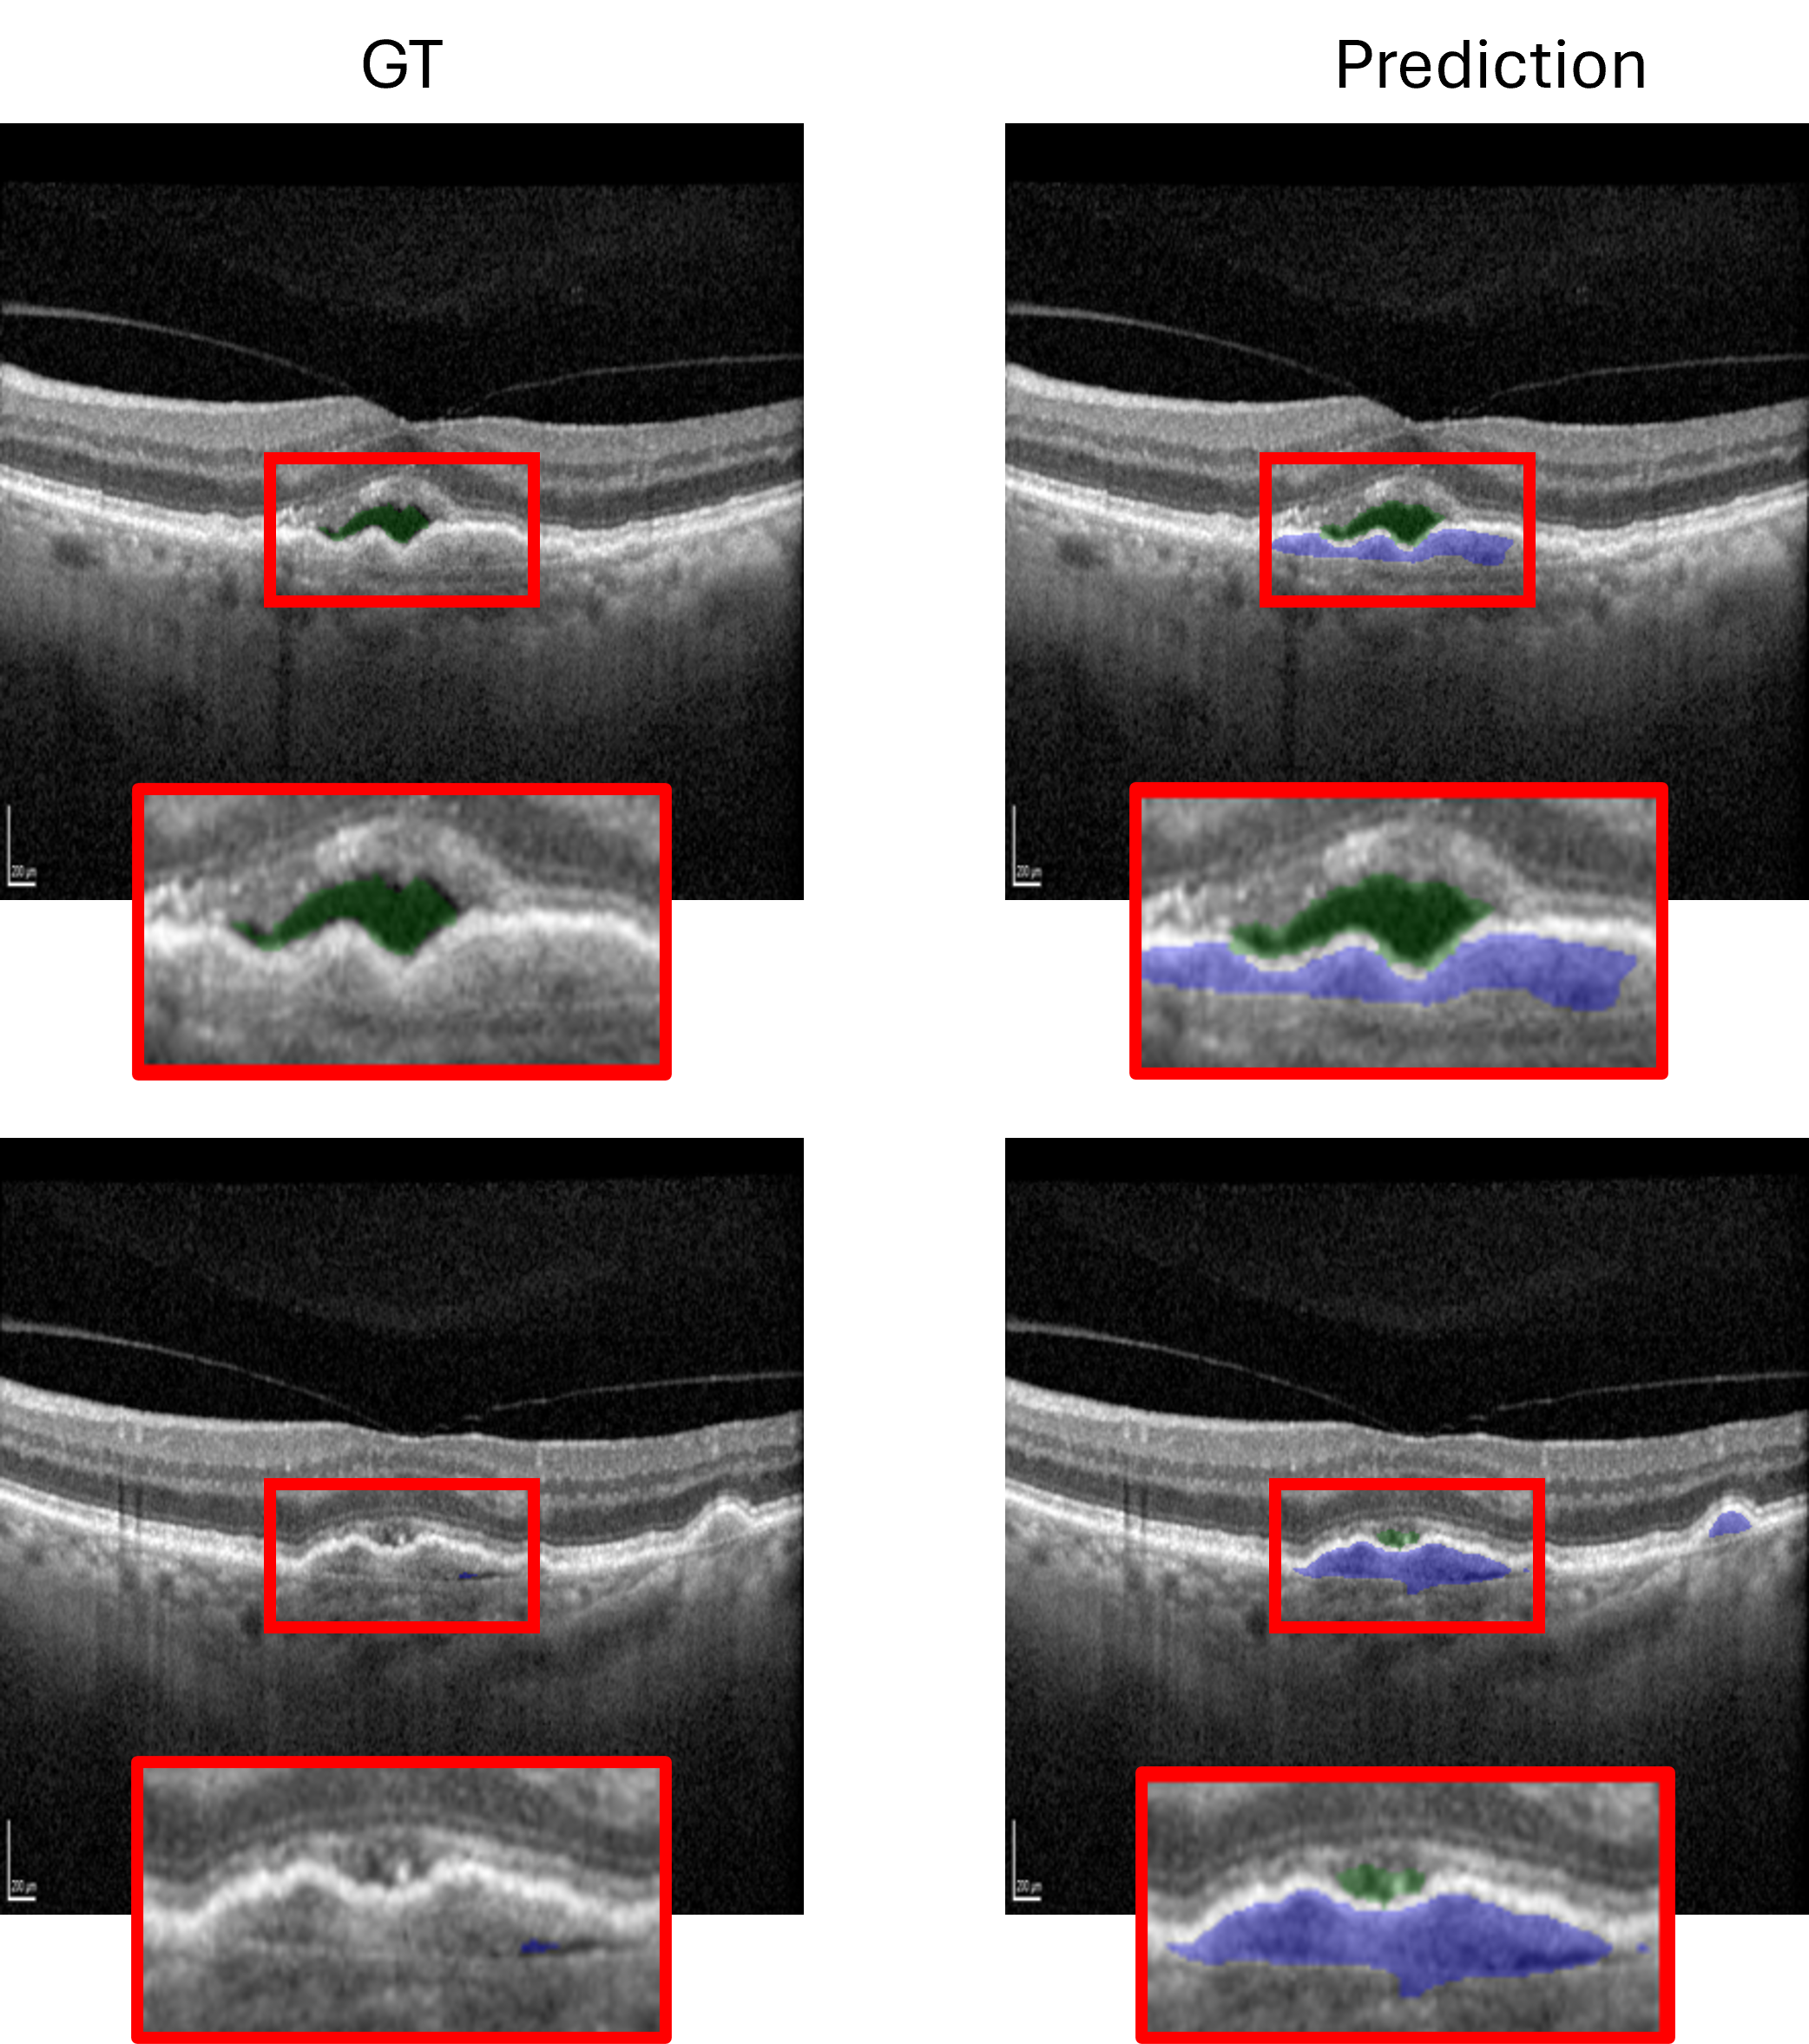
\includegraphics[width=0.65\linewidth]{figures/CHUSJPEDSegmentation.png}
	\caption{SRF and PED segmentation in two B-scans from CHUSJ. The regions segmented by the model as PED could also be considered fluid, depending on the criteria applied.}
	\label{fig:CHUSJPEDSegmentation}
\end{figure}

The segmentation of SRF was the most consistent in this dataset. While the Dice coefficients are smaller than those obtained in the RETOUCH dataset, a worse performance was expected in the CHUSJ, highlighted by its diversity of images and different criteria than those applied in RETOUCH. In Figure \ref{fig:CHUSJSRFSegmentation}, the segmentation of a B-scan with SRF is shown. While the segmentation by the model correctly identifies the SRF region, a slight oversegmentation is performed. This is seen across multiple B-scans, influenced by the data in which it was trained, resulting in a worse Dice score in the slices with fluid.

\begin{figure}[!ht]
	\centering
	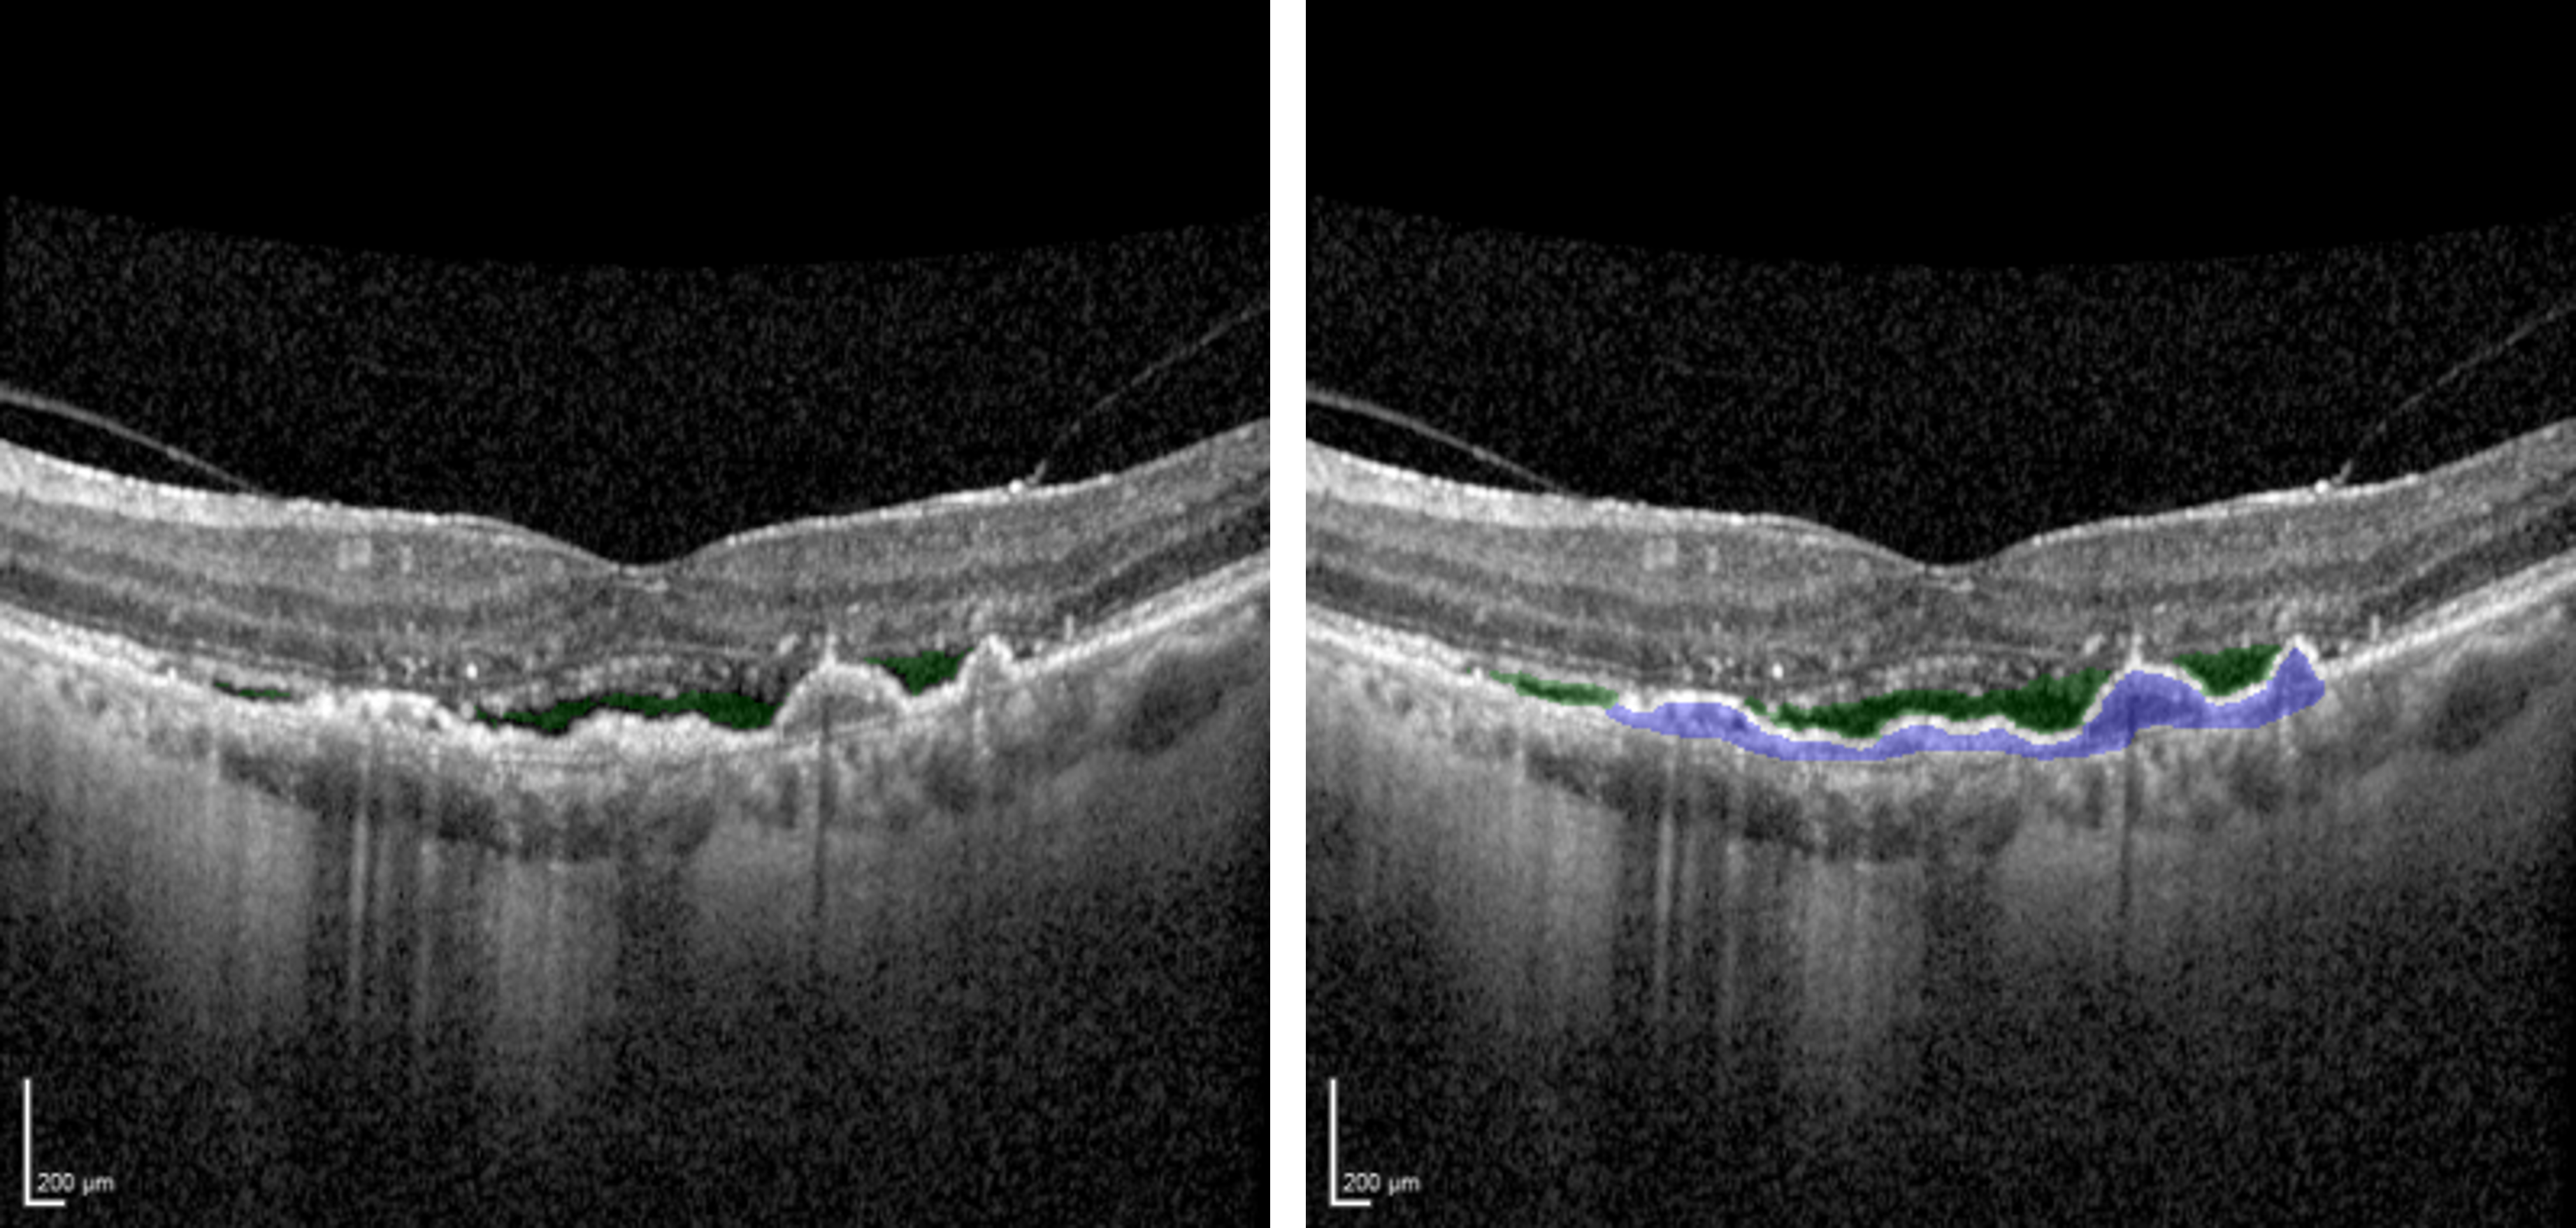
\includegraphics[width=0.60\linewidth]{figures/CHUSJSRFSegmentation.png}
	\caption{SRF and PED segmentation (right) in a B-scan from CHUSJ, compared to its GT (left). This shows the tendency to oversegmentation by the model.}
	\label{fig:CHUSJSRFSegmentation}
\end{figure}

Similar to SRF, the IRF segmentation is also decent in the slices which contain this fluid. Likewise, the model tends to slightly oversegment the fluid regions, as seen in Figure \ref{fig:CHUSJIRFSegmentation}. 

\begin{figure}[!ht]
	\centering
	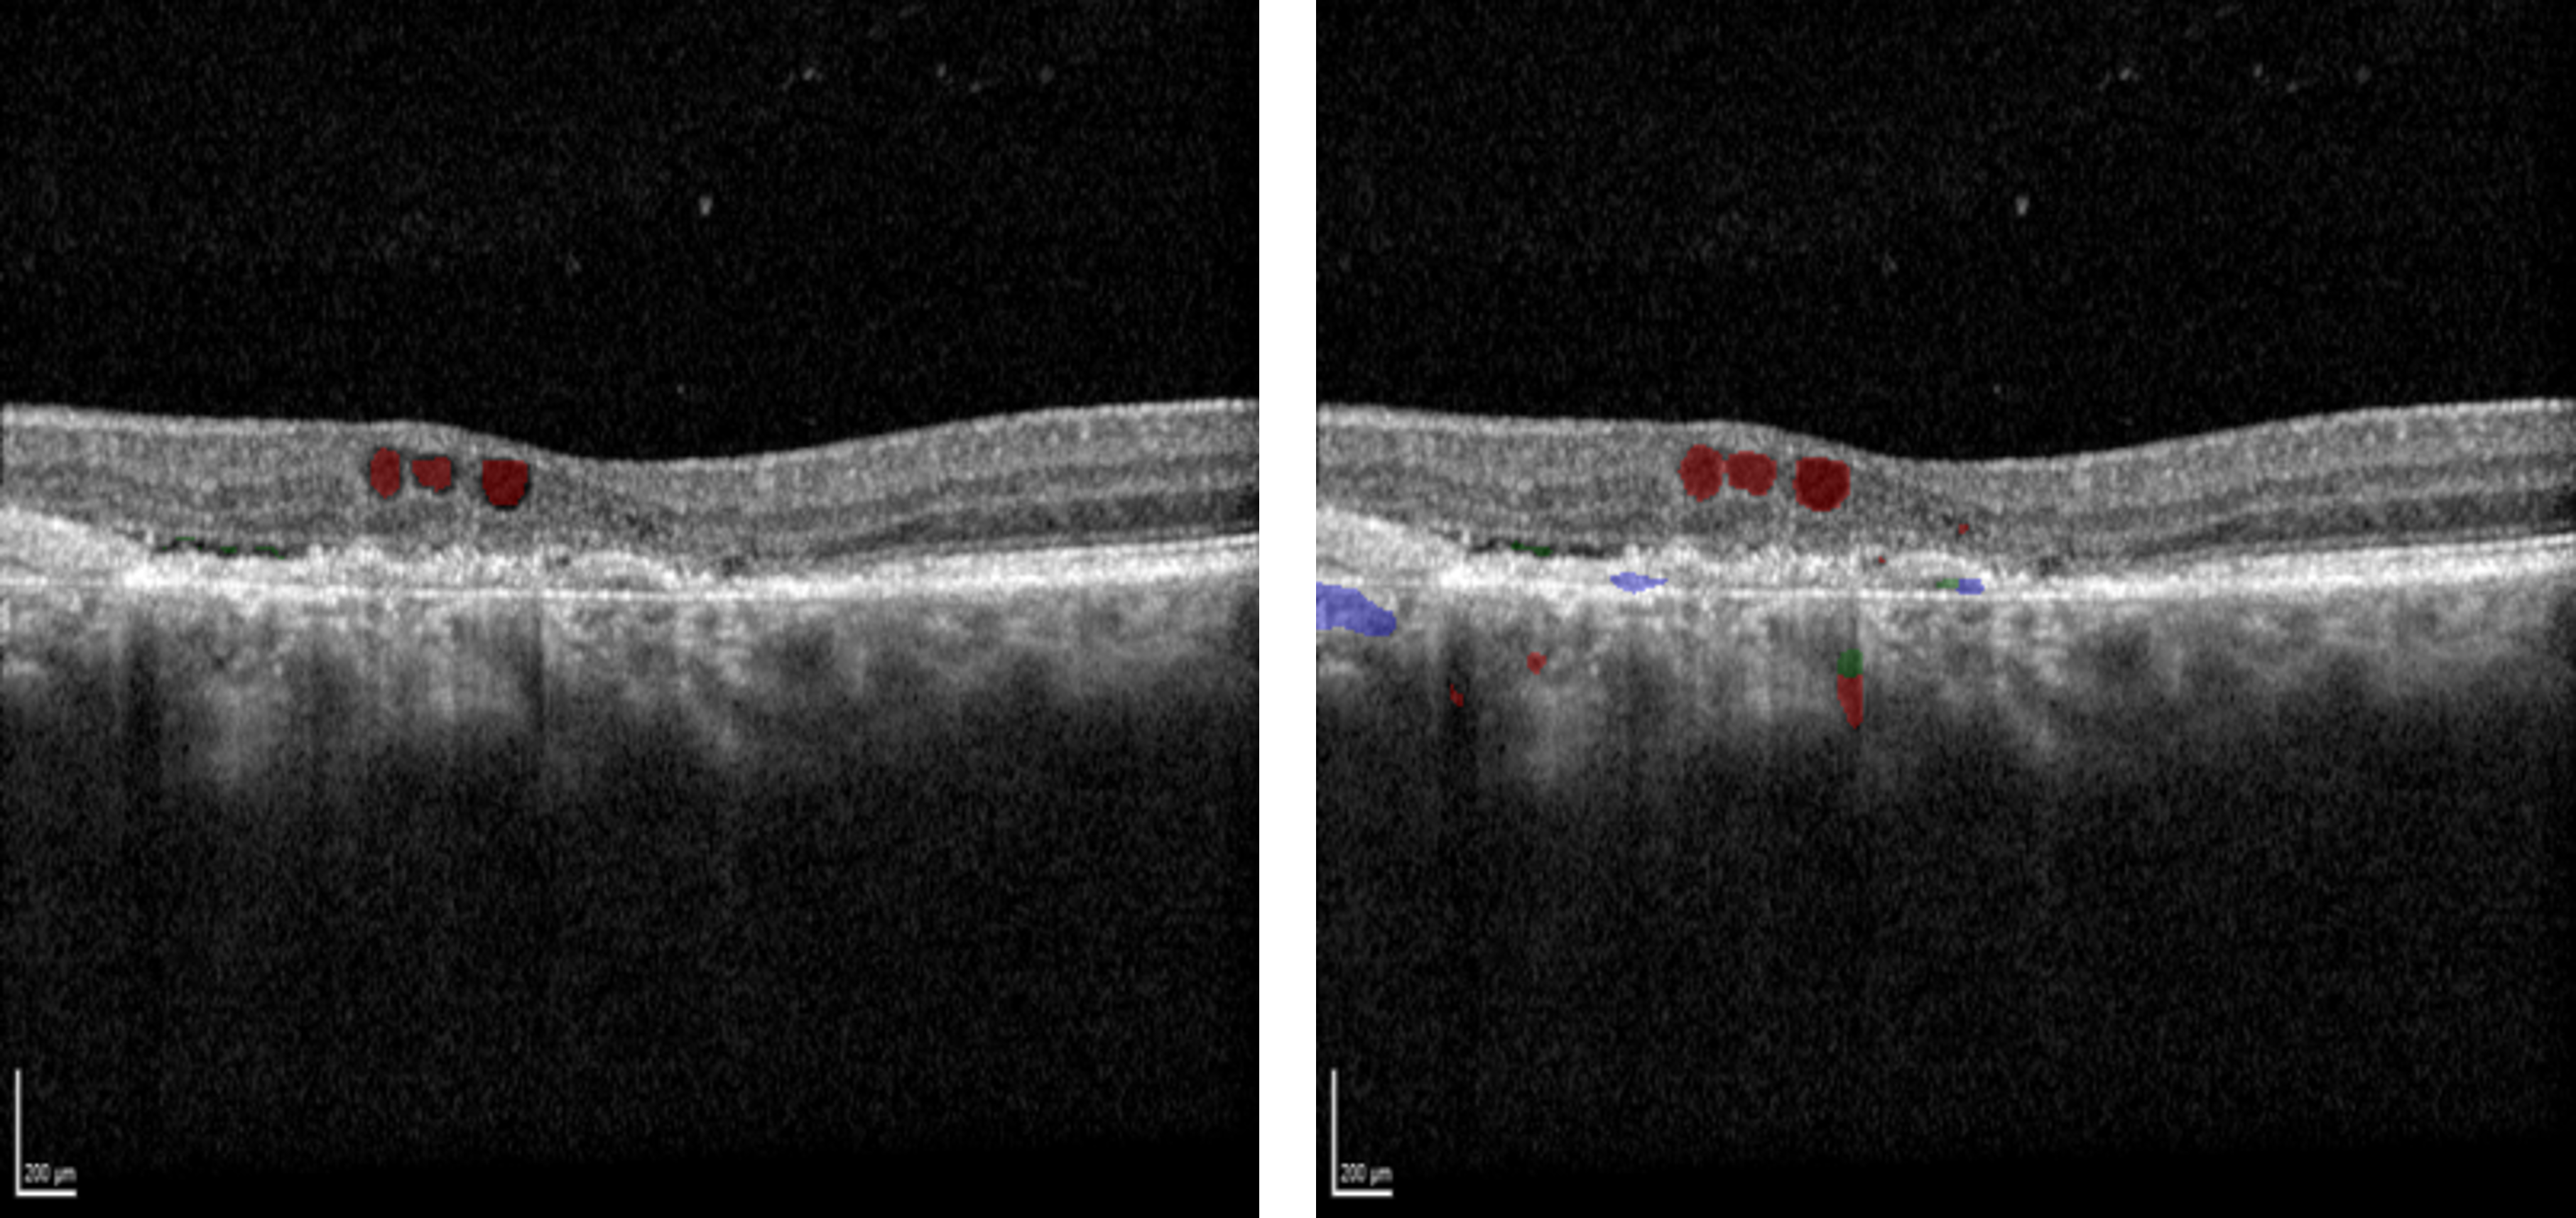
\includegraphics[width=0.60\linewidth]{figures/CHUSJIRFSegmentation.png}
	\caption{Segmentation of IRF regions (right) compared to its respective GT (left). The prediction of fluid regions in the choroid is also noticeable.}
	\label{fig:CHUSJIRFSegmentation}
\end{figure}

However, the main reason behind the poor Dice coefficients when considering all the slices is the fluid detection. In slices in which the fluids are not present, particularly in IRF and PED, they are still predicted outside the retina, usually in the choroid. While this is already visible in Figure \ref{fig:CHUSJIRFSegmentation}, where all the fluids are segmented in the choroid, more examples are shown in Figure \ref{fig:CHUSJChoroidSegmentation}.

\begin{figure}[!ht]
	\centering	\includegraphics[width=0.65\linewidth]{figures/CHUSJChoroidSegmentation.png}
	\caption{Segmentation of multiple fluids in the choroid region of the B-scans. This is performed often, significantly reducing the Dice coefficients seen in Table \ref{tab:CHUSJSegmentationResults}.}
	\label{fig:CHUSJChoroidSegmentation}
\end{figure}

The incorrect segmentations in the choroid are caused by the different quality of the image in this dataset. When training the segmentation models with the RETOUCH dataset, the Spectralis scans are focused on the retinal layers, blurring the structures outside of it, including the choroid. In the B-scans which compose the CHUSJ dataset, this region is not blurred. This confuses the segmentation model which also interpret the choroid as retina, thus predicting the existence of fluid regions there. The fluid which is the most affected by this segmentation is the IRF, due to the resemblance with the structures and intensities present in this region. Therefore, in case the region outside the retina was not considered in the final masks, the Dice coefficients would improve significantly. These segmentation errors are more prominent in the predictions performed by the binary models' segmentation as they present weaker capabilities of understanding anatomic references, basing their predictions more on the pixels intensities, thus being more easily fooled by the choroid.
\par
The use of resized images or their original shape did not translate to a significant difference in segmentation, as the performances remained almost unchanged when varying the slices shape. Since these transformations are applied along the horizontal axis, the different resolutions are harder to perceive, as they do not significantly change the perception of the structures in the B-scan.
\par
Lastly, the influence of the noise and different perceptions present in this dataset, as in the examples shown in Figure \ref{fig:CHUSJProblematicImages}, is more significant outside the retina. In Figure \ref{fig:CHUSJSegmentationOnNoisyScans}, the segmentation of these noisy B-scans is shown, where a decent segmentation of SRF is seen, with a prediction of PED coherent with the training data. However, it is outside the retina, in the choroid, where the wrong IRF segmentations are seen.

\begin{figure}[!ht]
	\centering	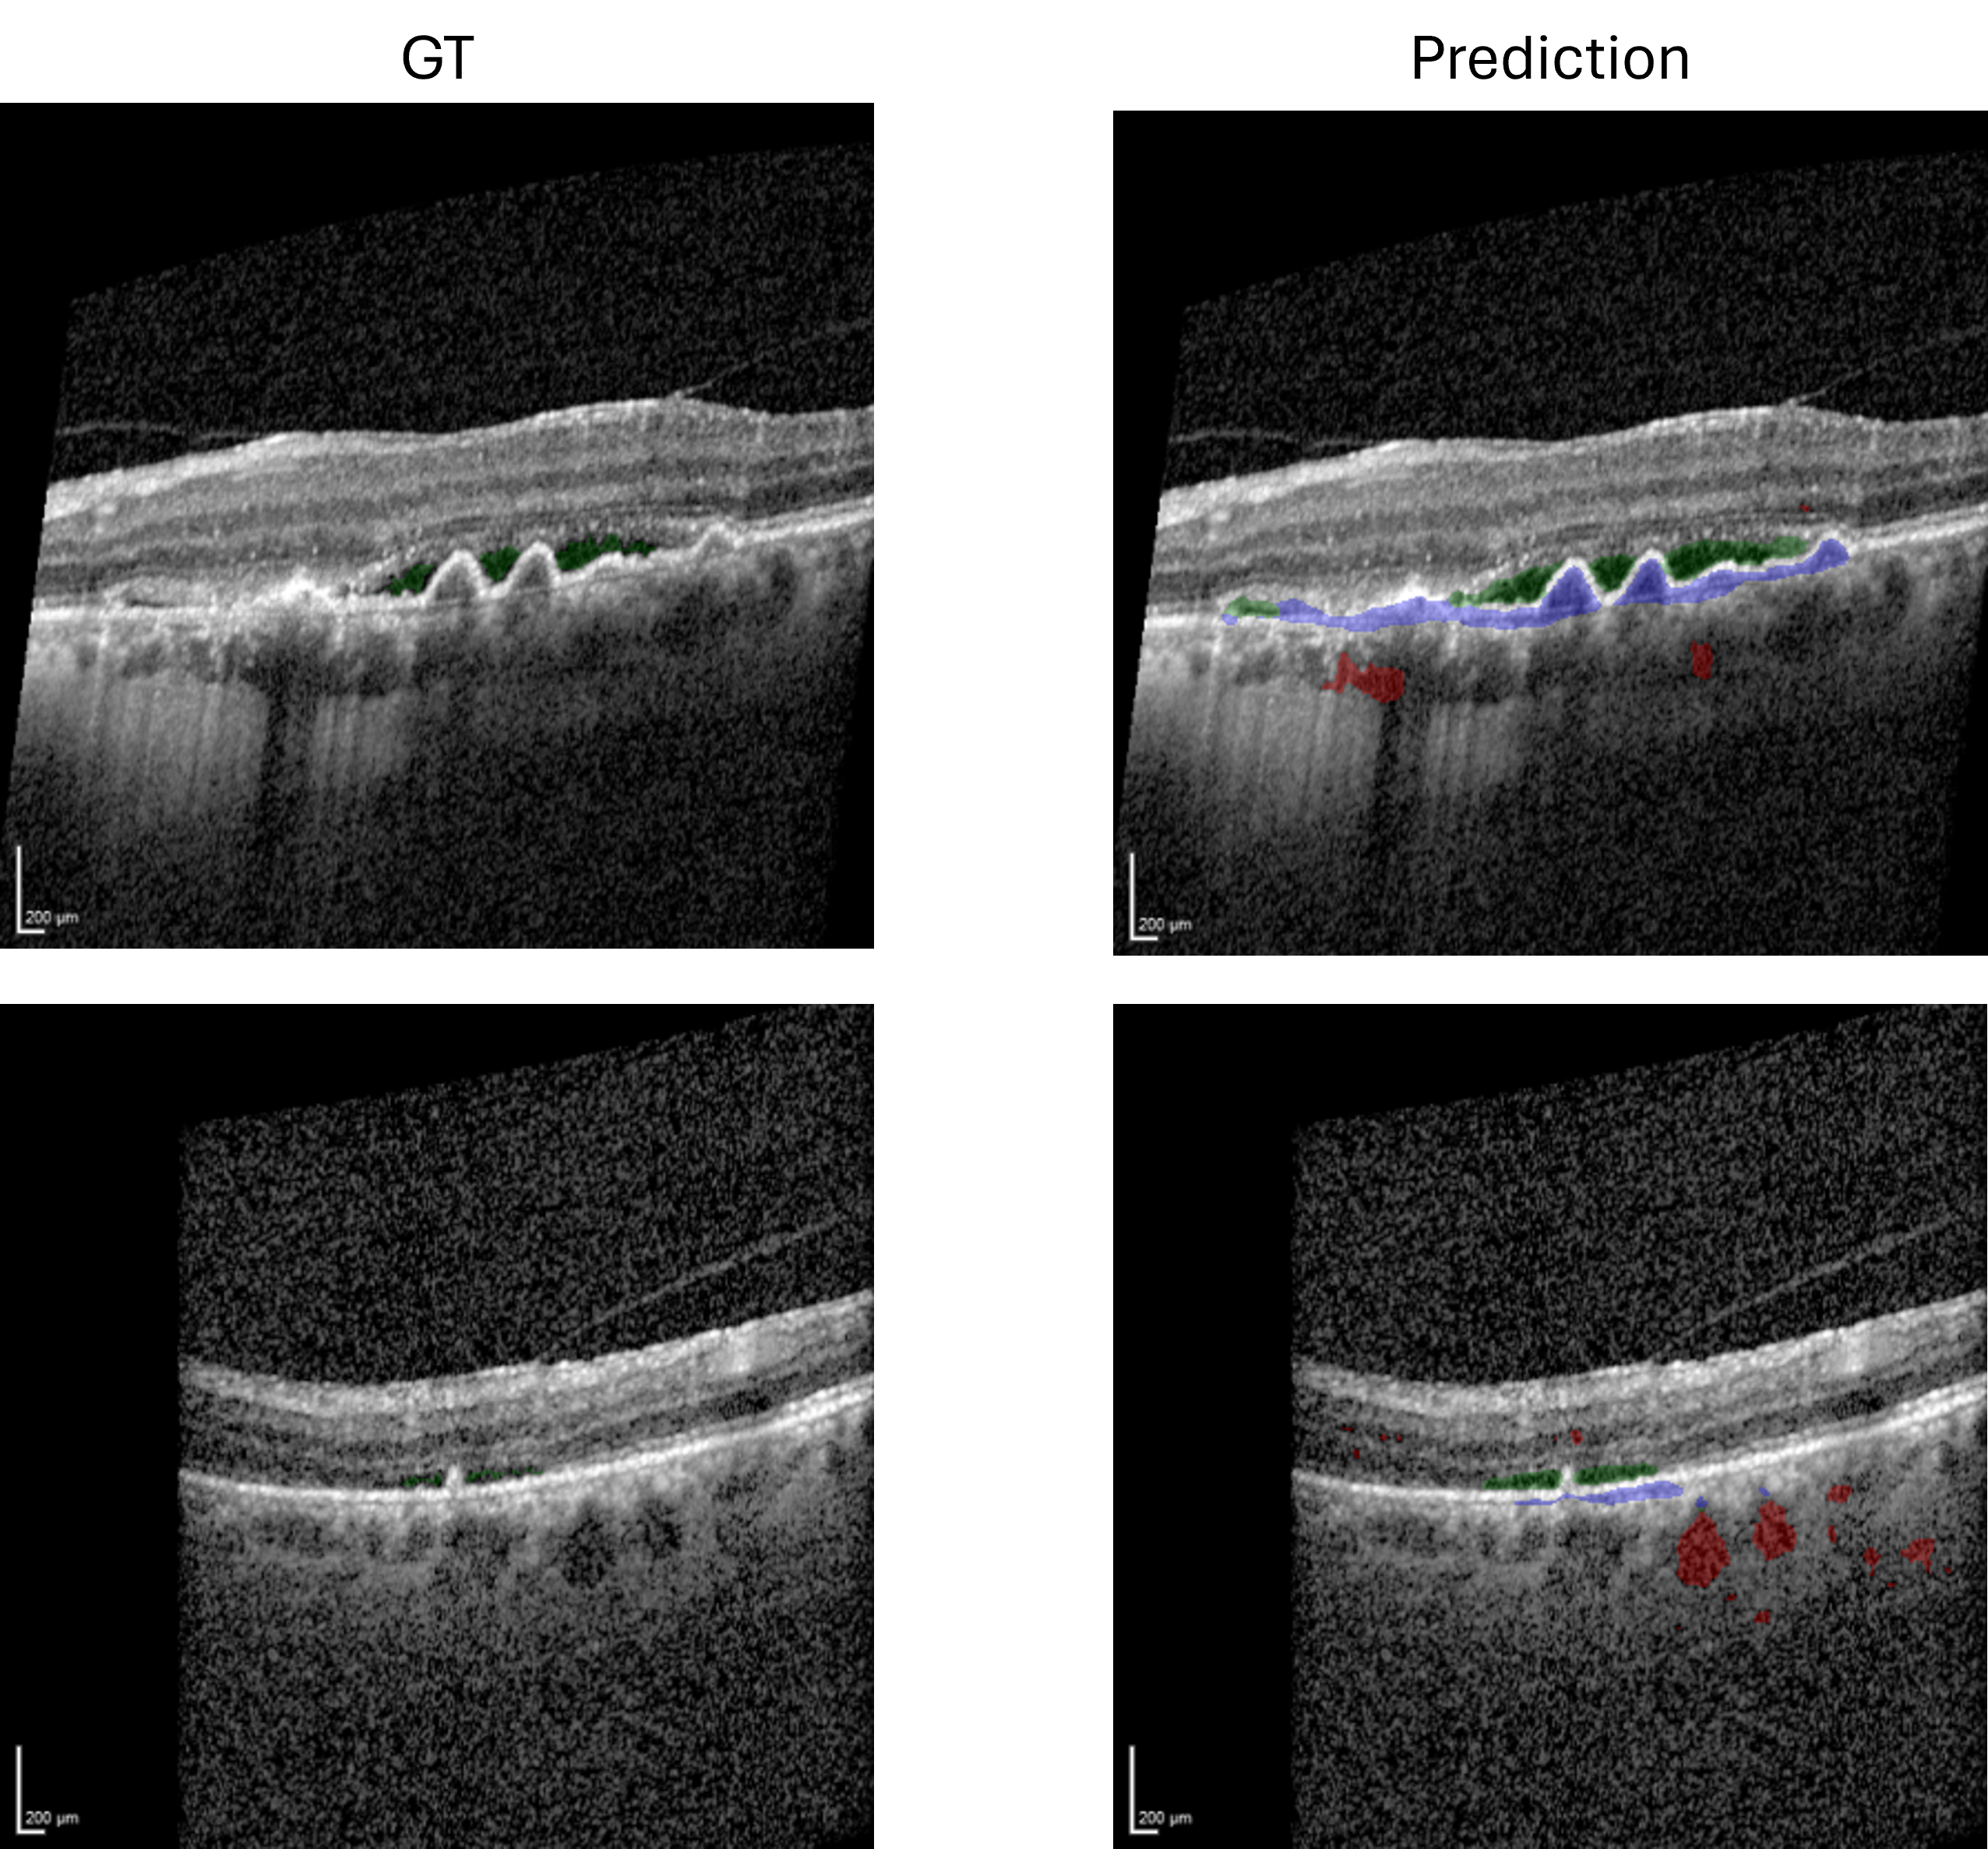
\includegraphics[width=0.75\linewidth]{figures/CHUSJSegmentationOnNoisyScans.png}
	\caption{Fluid segmentations performed by the multi-class model in noisy B-scans from the CHUSJ dataset.}
	\label{fig:CHUSJSegmentationOnNoisyScans}
\end{figure}

\section{Intermediate Slice Synthesis}\label{IntermediateSliceSynthesis}

This section presents the results obtained in the generation of intermediate B-scans between two consecutive real slices. In this section, the images generated using two different generative models are compared: the GAN and the U-Net.
\par
The comparison between these different methods is mainly qualitative, as the quality and perception of the images are prioritized over the calculated metrics, since the realism of the images and the performance of segmentation models on the generated slices are significantly affected by the appearance of the images.
\par
Nevertheless, the GANs trained on different folds are still compared through PSNR and SSIM, as a way to objectively select the best performing model for the \ref{FluidVolumeEstimation} Fluid Volume Estimation experiments.
\par
The comparison between these metrics and other articles in the literature is not possible. The only article of intermediate slice synthesis applied in OCT, developed by \textcite{Lopez2023}, does not evaluate the generated slices using these metrics. The articles in other imaging techniques such as CT and MRI have significantly different levels of noise and the values attained in these metrics in OCT are, therefore, very different.

\subsection{Experiment 3}

In Experiment 3, a GAN was trained with the objective of generating the intermediate slice between a pair of two known and consecutive slices. In Table \ref{tab:Experiment1Metrics}, the PSNR and SSIM are shown for each fold in which the network was trained.

\begin{table*}[!ht]
	\caption{PSNR and SSIM in every device, for the generated slices in every validation fold.}
	\centering
	\resizebox{\textwidth}{!}{\begin{tabular}{|c|c|cccc|c|cccc|c|}
		\hline
		\multirow{2}{*}{\textbf{Run}} & \multirow{2}{*}{\textbf{VF}} & \multicolumn{4}{c|}{\textbf{PSNR}} & \multirow{2}{*}{\textbf{PSNR}} & \multicolumn{4}{c|}{\textbf{SSIM}} & \multirow{2}{*}{\textbf{SSIM}} \\ \cline{3-6} \cline{8-11}
		&  & \textbf{Cirrus} & \textbf{Spectralis} & \textbf{T-1000} & \textbf{T-2000} &  & \textbf{Cirrus} & \textbf{Spectralis} & \textbf{T-1000} & \textbf{T-2000} &  \\ \hline
		\textbf{Run 1} & 2 & \multicolumn{1}{c|}{} & \multicolumn{1}{c|}{} & \multicolumn{1}{c|}{} & \multicolumn{1}{c|}{} &  & \multicolumn{1}{c|}{} & \multicolumn{1}{c|}{} & \multicolumn{1}{c|}{} & \multicolumn{1}{c|}{} &  \\
		\textbf{Run 2} & 3 & \multicolumn{1}{c|}{\textbf{20.44}} & \multicolumn{1}{c|}{24.58} & \multicolumn{1}{c|}{21.63} & \multicolumn{1}{c|}{22.24} & 21.69 & \multicolumn{1}{c|}{\textbf{0.181}} & \multicolumn{1}{c|}{0.484} & \multicolumn{1}{c|}{0.188} & \multicolumn{1}{c|}{0.246} & 0.247 \\
		\textbf{Run 3} & 4 & \multicolumn{1}{c|}{20.40} & \multicolumn{1}{c|}{\textbf{24.93}} & \multicolumn{1}{c|}{\textbf{21.95}} & \multicolumn{1}{c|}{\textbf{22.56}} & \textbf{21.91} & \multicolumn{1}{c|}{0.175} & \multicolumn{1}{c|}{\textbf{0.498}} & \multicolumn{1}{c|}{\textbf{0.228}} & \multicolumn{1}{c|}{\textbf{0.263}} & \textbf{0.257} \\
		\textbf{Run 4} & 0 & \multicolumn{1}{c|}{} & \multicolumn{1}{c|}{} & \multicolumn{1}{c|}{} & \multicolumn{1}{c|}{} &  & \multicolumn{1}{c|}{} & \multicolumn{1}{c|}{} & \multicolumn{1}{c|}{} &  &  \\
		\hline
		\hline
		\textbf{Set 1} & - & \multicolumn{1}{c|}{} & \multicolumn{1}{c|}{} & \multicolumn{1}{c|}{} & \multicolumn{1}{c|}{} &  & \multicolumn{1}{c|}{} & \multicolumn{1}{c|}{} & \multicolumn{1}{c|}{} & \multicolumn{1}{c|}{} &  \\ \hline
	\end{tabular}}
	\label{tab:Experiment1Metrics}
\end{table*}

One of the trends that becomes evident when looking at this table is the difference in results between devices, which is constant across independent of the fold in which it was trained.
\par
In every fold, the scans generated with the Spectralis device show better values both in PSNR and SSIM, while those obtained with Cirrus are significantly worse. This is tied to the characteristics of the images obtained with each device. In Spectralis, the inter-slice distance is larger than in Cirrus, but this is compensated by the better B-scan quality, contrast, and reduced levels of noise. The opposite happens in Cirrus, as the B-scans are noisier and with a decent contrast, but separated by a smaller distance. In Topcon, the distance is similar to the Cirrus, but presents less noise with worse contrast. 
\par
As the speckle noise is hard to predict due to its random nature, the performance metrics are worse in the scans with more noise. These metrics compare the similarity between different images at a pixel level and in noisy regions, which occupy most of the B-scan, the differences at a pixel-level between generated and real images are significant, even if the differences are almost imperceptible.
\par
In other imaging techniques like MRI and CT, the noise levels are much less significant than OCT, resulting in better PSNR and SSIM values, that directly translate to image quality.
\par
When comparing the results across different runs, it turns out that the performance changes very slightly when the training data differs. Unlike the segmentation task, where the results in different validation folds were harshly affected by the fluid content present in the OCT volumes that compose them, the generation task appears indifferent to the random distribution of fluid.
\par
In the segmentation task, the model and evaluation focused solely on the fluid, which is a small portion of the image, while in generation the model attempts to accurately generate the whole scan as similar to the target slice as possible. By considering the entirety of the B-scan, less of the performance is affected by the fluid region, which is why the distribution of fluid does not affect the overall performance as much as it did in segmentation, even if it is the most difficult section to generate.
\par
Despite the significant worse performance in Cirrus when compared to Spectralis, the visual similarity between generated images and real images, at an human level, is not very different. In Figure \ref{fig:GeneratedSlicesCirrusVsSpectralis}, two pairs of real and generated images from these devices are shown.
\par
The generated slices capture the rough idea of the image, especially the retinal layers, but miss on the small details such as noise patterns, and brighter and unexpected structures. Overall, the generated Cirrus scan captures the details present in the real image better than the Spectralis. For example, the structures which appear in the choroid are similar to the original slice in the generated Cirrus slice, while in Spectralis these structures appear blurred. However, due to the highest levels of noise, this does not translate to better PSNR or SSIM.

\begin{figure}[!ht]
	\centering	\includegraphics[width=0.75\linewidth]{figures/GeneratedSlicesCirrusVsSpectralis.png}
	\caption{Example of two pairs of generated slices, one from Cirrus and one from Spectralis, which capture the retinal layers.}
	\label{fig:GeneratedSlicesCirrusVsSpectralis}
\end{figure}

The differences in performance exhibited in this image regarding the representation of details are related with the inter-slice distance of the OCT volumes. In Cirrus, where the inter-slice distance is smaller than in Spectralis, the differences between the surrounding slices and the middle slice are smaller. Therefore, it is easier for the model to predict the content in the middle slice of a Cirrus volume than it is in Spectralis. Figure \ref{fig:TransitionBetweenConsecutiveBScansCirrusVsSpectralis} shows the surrounding slices of the B-scans generated in Figure \ref{fig:GeneratedSlicesCirrusVsSpectralis}. It becomes evident the difference in the transitions between the surrounding slices and the intermediate slices. For example, in the choroid region, where the generative model output was blurred, the structures that appear in the previous slice are significantly different in the following slice. In the same region, the Cirrus B-scans present a much smoother transition, which results in an improved and more realistic output.

\begin{figure}[!ht]
	\centering	\includegraphics[width=1.0\linewidth]{figures/TransitionBetweenConsecutiveBScansCirrusVsSpectralis.png}
	\caption{Surrounding slices of the B-scans generated in Figure \ref{fig:GeneratedSlicesCirrusVsSpectralis}.}
	\label{fig:TransitionBetweenConsecutiveBScansCirrusVsSpectralis}
\end{figure}

However, it is of our best interest to generate slices that accurately represent the fluid regions, on top of being visually similar to the original scans, as an accurate representation of the generated fluids, directly translates to a better performance in the segmentation of fluid in theses slices. 
\par
An accurate segmentation of fluid in generated B-scans is mainly dependent on the overall quality of the image and its resemblance to the images in which it was trained and the aspect of the generated fluid regions.
\par
Similar to what was seen in other structures such as the choroid and the retinal layers, the quality of the generated fluid regions is dependent on the distance between scans more than the contrast and levels of noise in the image. However, the characteristics of each fluid also influence its generation, mainly because of their progression between consecutive slices. For example, the SRF usually appears in a more homogeneous and continuous shape, making it easier to predict its characteristics given the information of the surrounding slices. Contrasting, the IRF usually appears in small and irregular shapes, commonly separated by small retinal tissue. In consecutive slices, the small IRF regions quickly change its shape and may even merge together, which makes it harder to predict. The PED fluid can appear both as small inconsistent fluid like the IRF, but most commonly as a large and predictable region, similar to SRF.
\par
An example of each generated fluid is seen in Figure \ref{fig:GeneratedSlicesWithFluid}, where the generation of IRF confuses the model while the fake SRF and PED appear similar to its GT. The characteristics of these generated fluids is particularly important to understand the consequences that slice generation has in fluid volume estimation.

\begin{figure}[!ht]
	\centering	\includegraphics[width=1.0\linewidth]{figures/GeneratedSlicesWithFluid.png}
	\caption{Examples of generated B-scans with fluid.}
	\label{fig:GeneratedSlicesWithFluid}
\end{figure}

In this figure, it becomes evident that the generation of SRF and PED, seen in Topcon example, is a much simpler task than the generation of any other fluid. In fact, the overall structure of this region has been very accurately preserved, apart from small visual details.
\par
The generation of IRF, however, appears more troublesome, particularly in Spectralis. In this last device, while in the GT the fluid regions appear individually separated by small retinal tissue, in the generated images the structures surrounding the fluid appear deformed, making it hard to understand which region is fluid and which is retina. It is interesting to note that the SRF shape stays consistent, highlighting that this fluid changes much slower as the slices progress than IRF. In Cirrus, the model preserves the IRF structures accurately, apart from the small and thin sections of retinal tissue which separate the fluid regions, where some merging occurs. This small details occur due to the target slice being located between one slice that contains this small tissues and another that does not. Nevertheless, the characteristics of this fluid are much more similar to the GT than in Spectralis, emphasizing the impact that the inter-slice distance has in slice generation.
\par
The poor generation of IRF is also partially related with the loss used to train the GAN. Since this network was adapted from a video frame interpolation application, the method is not prepared for datasets that contain as much noise as OCT does. In the video use case, it makes sense to use a loss function that primarily evaluates the images at a pixel level, while being complimented by a perception component, which is the adversarial loss, that corresponds to the capability of a fake image fooling the discriminator. However, in OCT, the speckle that corrupts the image makes it considerably more difficult to optimize a network to generate images that are similar at a pixel level, since this noise is impossible to predict. Therefore, as the network attempts to reproduce the noise that occupies most of the B-scans, it does not apply as much attention to the fluid as it should, particularly in IRF that needs it more. Ultimately, this results in visually similar images in the matters of noise and retinal layers, but worse in the generation of fluids.
\par
To perform the generation of intermediate slices in Experiment 6, the model from Run 3 was selected, as it obtained the best metrics in PSNR and SSIM.

\subsection{Experiment 4}

The second experiment in the scope of generating intermediate slices was performed using a U-Net and only a single model was trained. Examples of B-scans generated using this model are shown in Figure \ref{fig:GenerativeUNetResults}.

\begin{figure}[!ht]
	\centering	\includegraphics[width=1.0\linewidth]{figures/GenerativeUNetResults.png}
	\caption{B-scans generated using the U-Net. The images on the left show the original B-scan while those on the left are the corresponding generated slices.}
	\label{fig:GenerativeUNetResults}
\end{figure}

When evaluating the quality of the generated images, a noticeable lack of realism is observed, as these images often resemble a smoothed approximation of the GT. Despite the similarity in architecture between the generator used in the GAN and the U-Net, the second model could not reach a performance comparative with the GAN. The U-Net faces three significant challenges: its loss is not representative, it is trained with large images, and does not have a discriminator.
\par
The main problem comes from the network not being able to produce realistic images by reducing the loss. While the MAE is a good metric to compare two images, it does not perform well as the loss of a generative model in OCT. The reason MAE is insufficient to motivate the model to properly generate images is because the easiest, fastest, and safest way the model has of reducing the MAE in training is by creating blurred images, especially in noisy regions of the image.
\par
While these blurred images are not as realistic as the GT, the MAE is not as bad as it would be in case the model attempted to create images that are more visually similar to the real images. When dealing with OCT, a large portion of the image contains speckle noise, which is difficult to predict. Therefore, reaching results that are visually similar includes the representation of speckle noise in the intermediate slices, which results in a worse MAE.
\par
It is due to the inability of regularizing a generative model alone that the MAE was combined with other losses in the previous experiment. While this loss is important to represent the direct similarity between two images, it fails to capture the perception of the structures and visual similarity between images. This is why the MAE loss was attributed such small weight in Experiment 3.
\par
When comparing to the work by \textcite{Nishimoto2024}, in which this experiment was inspired, the dataset presented almost no noise in most images. Therefore, the generative task was simpler and the model was able to generalize significantly better, as the MAE was enough to promote an accurate slice interpolation. However, when facing images with more noise, caused by the presence of metal artifacts in the CT, the generation of slices performed worse than the linear interpolation. Therefore, while this model generates good images when the slices have almost no noise present, it lacks the robustness to generate images where noise appears.
\par
The use of a U-Net to generate intermediate B-scans is also harmed by the input it received. While in the GAN, the discriminator and the generator were trained with small patches of 64 $\times$ 64, the U-Net was trained with the entire image. Consequently, this motivates the U-Net to focus on the more general details of the image, rather than on the finer characteristics, as done in the GAN, ultimately contributing to the generation of less realistic images.
\par
Lastly, this model lacks the regularization brought by an external network which is, in the case of a GAN, the discriminator. With the inclusion of a discriminator, a perceptual component is added to the loss. This motivates the model to produce the images that are not only similar to the pixel level, but also visually accurate. Therefore, this results in an image where the textures are more realistic, even if the difference at a pixel level is worse.
\par
Nevertheless, it is seen in Figure \ref{fig:GenerativeUNetResults} that the borders of the fluid regions are preserved. This representation is not as difficult as the other components of the B-scan, but is better in the generation of SRF and PED, where the fluid regions are more homogeneous. In IRF, the shape of the fluid is bounded by the deformations caused inside the retina, which makes it harder to generate, leading to the fluid regions appearing significantly different from what is expected. Furthermore, the goal of generating intermediate slices was not only to generate images that are similar in the fluid regions, but also in the overall image, and for this reason, no other generative U-Net model was trained. The accurate delimitation of the generated fluids does not directly translate to a good segmentation performance in the created slices, since the image's overall different appearance could impact the segmentation model's performance.

\section{Fluid Volume Estimation}\label{FluidVolumeEstimation}

The experiments discussed in this section relate to the estimation of fluid volume using the segmentation masks of each B-scan in an OCT volume. In both experiments, the fluid volumes predicted using the segmentation models are compared to the fluid volumes calculated using the GT masks from the dataset, in the reserved fold. 
\par
This fold had not been seen by any segmentation or generative model and the GT fluid masks are available for all OCT scans.
\par
The discussion of these experiments aim to understand the applicability of enhancing the resolution of an OCT volume and how that affects the total fluid volume estimated, among other aspects such as the perception of the generated slices by the segmentation model.
\par
The results are shown in tables where for each considered OCT volume, the fluid volume estimated for each fluid type (IRF, SRF, and PED) is presented in mm$^{3}$. At the end of each table, the MAE is shown to resume the differences between the GT fluid volumes and the prediction.
\par
In Experiment 6, the Dice coefficient for the predict segmentation masks in fully generated OCT volumes is shown, allowing the comparison between the segmentation model's performance in real data and generated data, providing an insight on which fluids are affected the most the generation.
\par
Lastly, scatter plots are shown for each comparison between predictions, where the each of the fluids' volumes calculated for each OCT scan are compared with each other, providing an intuitive and visual representation of the differences associated with the used data.

\subsection{Experiment 5}
In Experiment 5, the fluid volume was calculated for each type of fluid in the OCT volumes from the reserved fold, using the previously described in \ref{Methods} Methods. The volume of each fluid, for each OCT volume in the reserved fold, is shown in Table \ref{tab:FluidVolumesExperiment5}, in mm$^{3}$. In Figure \ref{fig:FluidVolumeScatterExperiment5}, the comparison between the values calculated using the GT masks and the masks predicted by the segmentation model is shown, using the values present in this table.

\begin{table*}[!ht]
	\centering
	\caption{Volume of each fluid calculated for the masks segmented in the RETOUCH (GT) and the masks segmented by the best segmentation model from Experiment 1 and 2 (P). The volumes correspond to the total fluid volume in the OCT scan, in mm$^{3}$.}
	\begin{tabular}{|c|c|cc|cc|cc|}
		\hline
		\multirow{2}{*}{\textbf{Vendor}} & \multirow{2}{*}{\textbf{Volume}} & \multicolumn{2}{c|}{\textbf{IRF}} & \multicolumn{2}{c|}{\textbf{SRF}} & \multicolumn{2}{c|}{\textbf{PED}} \\ \cline{3-8} 
		& & \textbf{GT} & \textbf{P} & \textbf{GT} & \textbf{P} & \textbf{GT} & \textbf{P} \\ \hline
		 Cirrus & TRAIN002 & 0.228 & 0.373 & 0.008 & 0.013 & 0.000 & 0.000 \\
		 Cirrus & TRAIN012 & 0.000 & 0.001 & 0.704 & 0.673 & 0.888 & 0.946 \\
		 Cirrus & TRAIN014 & 0.000 & 0.000 & 0.517 & 0.575 & 0.332 & 0.252 \\
		 Cirrus & TRAIN016 & 0.771 & 1.129 & 0.000 & 0.000 & 0.000 & 0.000 \\
		 Spectralis & TRAIN027 & 0.937 & 1.071 & 0.096 & 0.132 & 0.000 & 0.001 \\
		 Spectralis & TRAIN033 & 0.254 & 0.380 & 0.314 & 0.307 & 0.367 & 0.471 \\
		 Spectralis & TRAIN039 & 0.622 & 0.839 & 0.000 & 0.000 & 0.000 & 0.000 \\
		 Spectralis & TRAIN042 & 0.002 & 0.009 & 1.900 & 1.875 & 0.603 & 0.771 \\
		 Spectralis & TRAIN048 & 0.328 & 0.446 & 0.000 & 0.008 & 0.000 & 0.000 \\
		 T-2000 & TRAIN062 & 0.047 & 0.058 & 0.000 & 0.000 & 0.000 & 0.000 \\
		 T-1000 & TRAIN063 & 0.000 & 0.011 & 0.747 & 0.568 & 0.034 & 0.110 \\
		 T-1000 & TRAIN064 & 0.058 & 0.060 & 0.000 & 0.003 & 0.000 & 0.075 \\
		 T-2000 & TRAIN067 & 0.188 & 0.170 & 0.000 & 0.000 & 0.000 & 0.000 \\
		 T-2000 & TRAIN068 & 0.406 & 0.550 & 0.004 & 0.006 & 0.000 & 0.008 \\ \hline
		 \multicolumn{2}{|c|}{\textbf{MAE}} & \multicolumn{2}{c|}{0.092} & \multicolumn{2}{c|}{0.025} & \multicolumn{2}{c|}{0.041} \\ \hline
		 
	\end{tabular}
	\label{tab:FluidVolumesExperiment5}
\end{table*}

\begin{figure}[!ht]
	\centering	\includegraphics[width=0.66\linewidth]{figures/FluidVolumeScatterExperiment5.png}
	\caption{Volume estimated for each fluid in OCT volume using the masks predicted by the segmentation model compared with the volumes calculated using the GT masks. The OCT scans considered are the same as in \ref{tab:FluidVolumesExperiment5} and the gray line marks the points in which the fluid volume in the GT is equal to the predicted.}
	\label{fig:FluidVolumeScatterExperiment5}
\end{figure}

The values shown in this table reveal the similarity between the fluid volumes estimated with the RETOUCH GT masks and the masks predicted by the selected segmentation model. However, there are some outliers and evident trends seen.
\par
For example, in IRF, there are multiple examples where the predicted quantity of fluid is significantly larger than the real quantity, such as in TRAIN002, TRAIN016, TRAIN039, and TRAIN048. These outliers appear mostly on Cirrus and Spectralis. In these vendors, the IRF presents more diverse shapes and deformity of the retina, which makes segmentation significantly harder than in Topcon, where the IRF appears much smaller and without deformation.
\par
In SRF and PED, the differences between the true and predicted quantity are not so significant, with the largest discrepancies being the SRF and PED in TRAIN063. The shape of these fluids in the OCT volumes present in this fold are more consistent with those seen in training, hence resulting in a more accurate segmentation.
\par
Overall, the volumes predicted in scans with considerable quantities of fluid tend to differ more with its GT. This happens due to the deformation in the retina that is associated with large quantities of fluid, making it harder to predict the segmentation masks.
\par
Nonetheless, the fluid prediction in slices with little to no fluid tends to be accurate, highlighting the good specificity and segmentation of small fluids previously seen in the segmentation model.
\par
Regarding the performances per vendor, there is no significant differences to note, as most of the differences in noticeable in these results are related to the different characteristics of the patients in each OCT.
\par
It is interesting to note that in discrepancies between the real volume and the predicted volume, the segmentation model tends to overpredict fluid, which is associated with the oversegmentation trend seen in the predictions performed by this model. This is an important aspect to note, as it is rooted to the segmentation criteria used in the training data, the RETOUCH dataset. This trend further justifies the oversegmentations seen by the model in the CHUSJ dataset.
\par
In the following subsection, the results shown in Table \ref{tab:FluidVolumesExperiment5} will be compared with the estimated fluid volumes obtained using only generated slices and in an enhanced volume, where between every known slice another slice is generated.

\subsection{Experiment 6}

The results obtained regarding fluid estimation with generated slices, in the scope of Experiment 6, are shown in Table  \ref{tab:FluidVolumesExperiment6}. In this table, four different fluid volume estimates are shown for each OCT volume in the reserved fold, separately for each fluid type. The first estimate, ``GT'', is obtained using the unchanged B-scans from each volume and the fluid masks provided in the RETOUCH dataset. The second estimate, ``P'', corresponds to the fluid masks predicted by the segmentation model in the unchanged B-scans of the same OCT volumes. Both predictions and fluid estimations were already presented in Experiment 5. In the third estimate, ``G'', the B-scans from the RETOUCH dataset are substituted with their corresponding generated B-scan, obtained using the selected GAN model. In these generated scans, the segmentation model predicts the fluid masks, from which the estimated volumes presented in this table are obtained. Lastly, in the fourth estimation ``E'', the original OCT volumes from the RETOUCH dataset are enhanced, as a B-scan is generated between every two consecutive slices. The segmentation model predicts the fluid masks both in the original and generated slices.
\par
In the last three rows of the table, multiple MAE are calculated to compare the results obtained in the multiple columns. The first row, shows the MAE between the estimations in the column ``GT'' and the estimations from the other columns. In the second row, the estimations performed using the segmentation model in column ``P'' are compared to the estimations made in the columns ``G'' and ``E'', while the third row compares the results obtained in these last two columns.

\begin{table*}[!ht]
	\centering
	\caption{Volume of each fluid calculated for the masks segmented in the RETOUCH (GT) and for the masks predicted by the best segmentation model in the original RETOUCH images (P), in the generated slices (G), and when the original dataset is enhanced, combining alternating the real images with B-scans generated between them (E). The volumes correspond to the total fluid volume in the OCT scan, in mm$^{3}$.}
	\resizebox{\textwidth}{!}{\begin{tabular}{|c|c|cccc|cccc|cccc|}
		\hline
		\multirow{2}{*}{\textbf{Vendor}} & \multirow{2}{*}{\textbf{Volume}} & \multicolumn{4}{c|}{\textbf{IRF}} & \multicolumn{4}{c|}{\textbf{SRF}} & \multicolumn{4}{c|}{\textbf{PED}} \\ \cline{3-14} 
		& & \textbf{GT} & \textbf{P} & \textbf{G} & \textbf{E} & \textbf{GT} & \textbf{P} & \textbf{G} & \textbf{E} & \textbf{GT} & \textbf{P} & \textbf{G} & \textbf{E} \\ \hline
		
 		Cirrus & TRAIN002 & 0.228 & 0.373 & 0.356 & 0.372 & 0.008 & 0.013 & 0.014 & 0.013 & 0.000 & 0.000 & 0.000 & 0.000 \\
 		
		Cirrus & TRAIN012 & 0.000 & 0.001 & 0.001 & 0.001 & 0.704 & 0.673 & 0.664 & 0.670 & 0.888 & 0.946 & 0.939 & 0.943 \\
		
		Cirrus & TRAIN014 & 0.000 & 0.000 & 0.001 & 0.003 & 0.517 & 0.575 & 0.561 & 0.572 & 0.332 & 0.252 & 0.207 & 0.227 \\
		
		Cirrus & TRAIN016 & 0.771 & 1.129 & 0.957 & 1.050 & 0.000 & 0.000 & 0.001 & 0.000 & 0.000 & 0.000 & 0.000 & 0.000 \\
		
 		Spectralis & TRAIN027 & 0.937 & 1.071 & 1.066 & 1.063 & 0.096 & 0.132 & 0.136 & 0.136 & 0.000 & 0.001 & 0.002 & 0.002 \\
 		
		Spectralis & TRAIN033 & 0.254 & 0.380 & 0.414 & 0.385 & 0.314 & 0.307 & 0.298 & 0.320 & 0.367 & 0.471 & 0.397 & 0.427 \\
		
		Spectralis & TRAIN039 & 0.622 & 0.839 & 0.726 & 0.779 & 0.000 & 0.000 & 0.002 & 0.000 & 0.000 & 0.000 & 0.000 & 0.000 \\
		
		Spectralis & TRAIN042 & 0.002 & 0.009 & 0.017 & 0.011 & 1.900 & 1.875 & 1.828 & 1.852 & 0.603 & 0.771 & 0.822 & 0.781 \\

		Spectralis & TRAIN048 & 0.328 & 0.446 & 0.336 & 0.398 & 0.000 & 0.008 & 0.013 & 0.009 & 0.000 & 0.000 & 0.001 & 0.001 \\

		T-2000 & TRAIN062 & 0.047 & 0.058 & 0.043 & 0.051 & 0.000 & 0.000 & 0.000 & 0.000 & 0.000 & 0.000 & 0.000 & 0.000 \\

		T-1000 & TRAIN063 & 0.000 & 0.011 & 0.007 & 0.010 & 0.747 & 0.568 & 0.507 & 0.546 & 0.034 & 0.110 & 0.111 & 0.108 \\
		
		T-1000 & TRAIN064 & 0.058 & 0.060 & 0.061 & 0.063 & 0.000 & 0.003 & 0.025 & 0.008 & 0.000 & 0.075 & 0.215 & 0.114 \\

		T-2000 & TRAIN067 & 0.188 & 0.170 & 0.137 & 0.160 & 0.000 & 0.000 & 0.000 & 0.000 & 0.000 & 0.000 & 0.000 & 0.000 \\

		T-2000 & TRAIN068 & 0.406 & 0.550 & 0.543 & 0.548 & 0.004 & 0.006 & 0.006 & 0.006 & 0.000 & 0.008 & 0.010 & 0.008 \\
		
		\hline
		\multicolumn{2}{|c|}{\textbf{MAE compared to GT}} & - & 0.092 & 0.067 & 0.079 & - & 0.025 & 0.036 & 0.029 & - & 0.041 & 0.052 & 0.043 \\ 
		\multicolumn{2}{|c|}{\textbf{MAE compared to P}} & - & - & 0.037 & 0.016 & - & - & 0.012 & 0.005 & - & - & 0.023 & 0.009 \\
		\multicolumn{2}{|c|}{\textbf{MAE compared to G}} & - & - & - & 0.022 & - & - & - & 0.009 & - & - & - & 0.014 \\ 
		\hline
		
	\end{tabular}}
	\label{tab:FluidVolumesExperiment6}
\end{table*}

In Figures \ref{fig:Experiment6GTvsAll}, \ref{fig:Experiment6PredictedVsAll}, and \ref{fig:Experiment6GeneratedVsEnhanced}, the estimated volumes shown in Table \ref{tab:FluidVolumesExperiment6} are plotted and compared with each other, providing a visual insight in the relationships between the estimated fluids, making the analysis easier. Figure \ref{fig:Experiment6GTvsAll} compares the volumes estimated using the GT masks with the volumes estimated in the other columns, ``P'', ``G'', and ``E''. Similarly, Figure \ref{fig:Experiment6PredictedVsAll} confronts the fluid volume estimations made using the fluid masks predicted by the segmentation model to the estimations made in columns ``G'' and ``E''. Finally, Figure \ref{fig:Experiment6GeneratedVsEnhanced} confronts the fluid volumes predicted in the generated dataset to the fluid volumes predicted in the enhanced dataset.

\begin{figure}[!ht]
	\centering	
	\includegraphics[width=1.0\linewidth]{figures/Experiment6GTvsAll.png}
	\caption{Volume estimated for each fluid in the OCT volumes using the GT masks, compared with the volumes estimated in columns ``P'', ``G'', and ``E''.}
	\label{fig:Experiment6GTvsAll}
\end{figure}

\begin{figure}[!ht]
	\centering	\includegraphics[width=1.0\linewidth]{figures/Experiment6PredictedVsAll.png}
	\caption{Volume estimated for each fluid in the OCT volumes using the masks predicted by the segmentation model compared with the volumes calculated using the masks from columns ``G'' and ``E''.}
	\label{fig:Experiment6PredictedVsAll}
\end{figure}

\begin{figure}[!ht]
	\centering	\includegraphics[width=0.50\linewidth]{figures/Experiment6GeneratedVsEnhanced.png}
	\caption{Volume estimated for each fluid in the OCT volumes using the masks predicted by the segmentation model in the generated dataset, compared with the volumes calculated in the enhanced dataset.}
	\label{fig:Experiment6GeneratedVsEnhanced}
\end{figure}

Considering the information exposed in the previous table and figures, many conclusions can be drawn regarding fluid volume estimation. For example, the differences between columns in the estimated fluid volumes, are always larger in IRF. The generation of this fluid was seen in Experiment 3, to be the most difficult, due to the finer details that change in the transitions between consecutive B-scans. Combined with the worse quality in the generated slices, the segmentation of this fluid was also seen to be the most difficult fluid to segment in the volumes from this fold, as shown in Table \ref{tab:Experiment1VsExperiment2}, where the IRF Dice coefficient is lower than in any other fluid. Both aspects significantly influence the estimation of this fluid in the unseen data. 
\par
The SRF presents the smallest differences between columns, as the MAE in this fluid are smaller than in any other fluid. The fluid estimation of SRF benefits from the accurate representation of this fluid in the generated slices, due to its uniform, homogeneous, and predictable characteristics, as seen in Experiment 3. Contrary to IRF, the segmentation model performs exceptionally well in the segmentation of SRF, when compared to the other fluids. Therefore, an accurate representation of the SRF masks is obtained, leading to an accurate fluid estimation.
\par
The estimation of the PED volume appears as an intermediate performance between the other two fluids. The segmentation of this fluid is better than IRF, but worse than PED, while its representation in generated slices is accurate when presented in large regions, but not so good when appearing in small regions. This translates to a smaller deviation between columns when comparing to IRF, but not as good as SRF.
\par
The differences between the columns ``GT'' and ``P'' are inherent to the capability of the segmentation model. This model's capabilities also limit the accuracy of the estimated volumes in the generated and enhanced datasets, as the masks predicted in the generated slices are obtained using this model. Therefore, to understand the effect that generating slices has in total fluid volume estimation, it is important to observe the differences between the ``P'', ``G'', and ``E'' columns. 
\par
The differences between these columns are much smaller than the differences calculated when comparing these results to the GT. This indicates that the fluid estimation is more limited by the segmentation model, than it is by the generated slices. This is particularly true when comparing column ``P'' to column ``E'', as illustrated in Figure \ref{fig:Experiment6PredictedVsAll}. In this figure, most of the points appear close to the gray line, which indicates that the fluid volumes predicted when adding the generated slices are similar to the fluid volumes estimated when predicting the segmentation masks in the original RETOUCH dataset.
\par
To isolate the impact of the generated slices in the fluid estimation, it is more important to look at the differences between the fluids estimated in columns ``P'' and ``G'', as well as Figures \ref{fig:Experiment6PredictedVsAll} and \ref{fig:Experiment6GeneratedVsEnhanced}. By observing this data, it becomes evident the similarity between performances in these datasets. In the SRF fluid estimation, the values are particularly similar, as well as in most cases of PED. However, it is in IRF where the largest differences appear, where the predictions of IRF by the segmentation model are of less quantity in the generated dataset.
\par
As seen in Experiment 3, IRF is the most difficult fluid to generate and attempts to recreate this fluid in intermediate slice, originate structures that do not resemble the IRF fluid. As a result, the segmentation models do not perceive this generated regions as IRF and do not segment them. This trend also seen in Figure \ref{fig:Experiment6PredictedVsAll} in the comparison between the original dataset and the enhanced dataset, where the largest differences appear in the segmentation of IRF, as the segmentation model predicts less fluid in the generated slices. However, since these B-scans are also mixed with original B-scans to form the OCT volume, the resulting differences are less significant.
\par
It is interesting to note that of the three biggest differences in IRF between the columns ``P'' and ``E'', TRAIN016, TRAIN039, and TRAIN048, which are highlighted in Figure \ref{fig:Experiment6PredictedVsAll} as the furthest points from the gray line, are in OCT volumes obtained with the Spectralis device. This trend is related with the larger inter-slice distance in Spectralis than in any other device, which makes it harder to create accurate IRF regions, which is amplified by this fluid's characteristics.
\par
In Table \ref{tab:Experiment6DiceInGeneratedDataset}, the Dice coefficients is calculated for the predicted masks in the generated dataset. These predicted fluid masks are compared to the real GT masks of the equivalent slices. The information shown in this table helps the understanding of which fluids' segmentation and which vendors are the most affected by generating intermediate slices and how these slices are understood by the model.

\begin{table*}[!ht]
	\caption{Comparison in Dice scores for every vendor and fluid in the reserved fold (fold 1), using the best segmentation model to segment the original B-scans and their generated equivalent.}
	\centering
	\resizebox{\textwidth}{!}{\begin{tabular}{|c|c|c|ccc|ccc|ccc|c|c|c|c|}
			\hline
			% Headers
			\multirow{2}{*}{\textbf{OCT Volumes}} &
			\multirow{2}{*}{\textbf{Slices}} &  
			\multirow{2}{*}{\textbf{VF}} & 
			\multicolumn{3}{c|}{\textbf{Cirrus}} & 
			\multicolumn{3}{c|}{\textbf{Spectralis}} & 
			\multicolumn{3}{c|}{\textbf{Topcon}} & 
			\multicolumn{1}{c|}{\multirow{2}{*}{\textbf{IRF}}} & 
			\multirow{2}{*}{\textbf{SRF}} & 
			\multirow{2}{*}{\textbf{PED}} & 
			\multirow{2}{*}{\textbf{Fluid}} \\ \cline{4-12} & & &
			\multicolumn{1}{c}{\textbf{IRF}} & 
			\multicolumn{1}{c}{\textbf{SRF}} & 
			\textbf{\textbf{PED}} & 
			\multicolumn{1}{c}{\textbf{IRF}} & 
			\multicolumn{1}{c}{\textbf{SRF}} & 
			\textbf{PED} & 
			\textbf{IRF} & 
			\textbf{SRF} & 
			\textbf{PED} & 
			\multicolumn{1}{c|}{} & & & \\ 
			
			\hline
			
			\multirow{3}{*}{\textbf{Original}} & All & 1 & 0.852 & 0.918 & 0.934 & 0.645 & 0.821 & 0.852 & 0.818 & 0.929 & 0.755 & 0.799 & 0.905 & 0.841 & 0.742 \\
			
			
			& Fluid & 1 & 0.654 & 0.799 & 0.767 & 0.645 & 0.687 & 0.703 & 0.624 & 0.744 & 0.588 & 0.641 & 0.756 & 0.716 & 0.702 \\
			
			
			& No Fluid & 1 & 0.941 & 0.972 & 0.978 & 0.646 & 0.889 & 0.885 & 0.884 & 0.960 & 0.766 & 0.873 & 0.952 & 0.862 & 0.786 \\	
			
			\hline
			\hline
			
			\multirow{3}{*}{\textbf{Generated}} & All & 1 & 0.740 & 0.896 & 0.903 & 0.307 & 0.707 & 0.850 & 0.763 & 0.870 & 0.726 & 0.671 & 0.850 & 0.816 & 0.627 \\
			
			
			& Fluid & 1 & 0.431 & 0.762 & 0.710 & 0.315 & 0.580 & 0.627 & 0.457 & 0.670 & 0.538 & 0.407 & 0.692 & 0.656 & 0.542 \\
			
			
			& No Fluid & 1 & 0.879 & 0.957 & 0.953 & 0.299 & 0.772 & 0.900 & 0.867 & 0.903 & 0.738 & 0.793 & 0.901 & 0.843 & 0.722 \\
			
			\hline
			
	\end{tabular}}
	\label{tab:Experiment6DiceInGeneratedDataset}
\end{table*}

As expected, the segmentation model performs better in the original dataset, where the structures present in the B-scans are the most similar to those seen in training. Nevertheless, in some metrics, the differences between the generated slices and the original slices is larger than in others.
\par
Regarding the segmentation of slices without fluid, the segmentation model behaves almost similarly to what is seen in the original data in most fluids and vendors. However, there are some exceptions, particularly in IRF and slices from Spectralis. Of all fluids, it is in IRF where the detection of fluid changes the most. This is due to the quality of the generated scans in IRF regions: since this area is harder to predict, the model outputs fluid regions that visually do not resemble IRF, leading the segmentation model to not predict this region as fluid. This particularly affects Spectralis, where the distance between slices is larger, making it harder to interpolate an intermediate slice. For this same reasons, the detection of SRF is affected, particularly due to the poor generation of small SRF regions.
\par
However, it is in the segmentation of slices with fluid where the performances significantly decrease. The segmentation of SRF and PED is not very affected by the generated slices in Cirrus and Topcon when compared to the other fluids. As seen in Experiment 3, the overall shape and characteristics of these fluids are easier to interpolate than IRF, as their structure is constant and homogeneous, with smooth transitions between consecutive slices, particularly in these vendors where the interslice distance is smaller.
\par
Again, the Spectralis generated slices are the ones that result in the largest decrement of segmentation performance in IRF and SRF. As stated previously, the reason behind this poor segmentation is tied to the poor generation of slices when compared to other vendors, which is related to the distance between consecutive slices. The reasons that cause the poor segmentation of the slices with IRF and SRF are the same reasons that lead to the oversegmentation of these fluids in B-scans that do not contain the fluids.
\par
One of the most noticeable outliers of the IRF volume estimation is the Spectralis volume TRAIN039. In Figure \ref{fig:SpectralisTrain039GenerationAndSegmentation}, the segmentation of IRF, as well as two generated slices, are shown.

\begin{figure}[!ht]
	\centering	\includegraphics[width=1.0\linewidth]{figures/SpectralisTrain039GenerationAndSegmentation.png}
	\caption{Example of IRF segmentation in the enhanced volume TRAIN039.}
	\label{fig:SpectralisTrain039GenerationAndSegmentation}
\end{figure}

It is visible in this figure that the second generated slice does not clearly represent the IRF region, as it appears slightly blurred and a large portion of the information does not resemble any structure present in the training images. For this reason, the segmentation model predicts a small area of fluid as IRF in this slice. The predicted area is much smaller than the area of IRF in the surrounding slices. This indicates that the area segmented is not coherent with the information in the surrounding slices, leading to an incorrect predicted fluid volume. The same occurs in the first generated slice of the shown example, but only a smaller portion of the image is unintelligible. 
\par
These two different situations further highlight that the rough transitions particularly affect the slices with small fluid regions, as the model is not capable of predicting which of these regions will appear in the intermediate slice.
\par
In the presented example, a single example of incorrect segmentation due to a poorly generated slice is shown, but multiple examples such as this appear in the predictions made in the mentioned enhanced volume. Accumulating this errors from multiple slices, results in a small total fluid volume than in the predictions made in the original dataset. This explains the decrease in total IRF segmented in the enhanced Spectralis volume when compared to the predictions in the original volume, as seen in Table \ref{tab:FluidVolumesExperiment6}.
\par
Figure \ref{fig:CirrusTrain012GenerationAndSegmentation} shows the segmentation of large SRF and PED volumes in the enhanced Cirrus TRAIN012 volume.

\begin{figure}[!ht]
	\centering	\includegraphics[width=1.0\linewidth]{figures/CirrusTrain012GenerationAndSegmentation.png}
	\caption{Example of SRF and PED segmentation in the enhanced volume TRAIN012.}
	\label{fig:CirrusTrain012GenerationAndSegmentation}
\end{figure}

In the shown generated images, the overall structure of the SRF and PED fluids is easier to accurately represent in the intermediate slices. Not only the transitions are smoother due to the smaller inter-slice distance in the Cirrus volumes, but also because of their homogeneous and regular shapes. Small artifacts that are seen in the GT slices are not represented in the intermediate slice, as they are unpredictable.
\par
As the generated fluid regions show the appearance that is characteristics of the true fluid regions in the original scans that compose the RETOUCH dataset, its segmentation is visually similar to the segmentation performed in the surrounding slices, which resemble the GT masks of the surrounding slices. 
\par
This example shows an accurate segmentation and generation of an enhanced OCT volume. This is a sample of segmentation and generation in the TRAIN012 volume, but most slices are segmented and generated as accurately as the shown example. This results in predicted fluid volumes that are similar to those estimated with the GT masks and with the predicted masks in the unchanged OCT volume.
\chapter{Conclusion}\label{Conclusion}

Throughout this dissertation, two main tasks were tackled in retinal OCT: fluid segmentation and intermediate slice generation. Theses tasks were explored with the goal of improving the automatic retinal fluid characterization, which includes the segmentation, identification, and quantification of IRF, SRF, and PED. This final chapter revisits the key findings and insights obtained from the experiments performed, presenting the strengths and limitations of the proposed methods.
\par
In the first experiments, multiple approaches to the multi-class segmentation were studied. The segmentation experiments started with a baseline U-Net, used in the multi-class segmentation of fluids. While  still using this network, the input was changed, testing different patch shapes and extraction procedures, which provided an insight on how each affects the network performance.
\par
When using smaller patches, extracted predominantly from the retina, the U-Net failed to understand the anatomic boundaries and relationships that define the retina, limited by the area of the image captured in this input. Therefore, the model would often segment outside of the retina and predictions while different fluids would be attributed to similar regions.
\par
The use of larger patches, which occupied the majority of each the B-scan, significantly improved the model's performance, but did not solve all the problems seen in smaller patches. While the model better understood the limits imposed by the retinal layers and learned how to leverage these landmarks in segmentation, the segmentations lacked detail in smaller regions. This is a common issue in models trained with the full image or larger patches. The model learns the bigger features better, such as the relationships between layers and fluids, but fails to grasp the smaller details, such as small fluid regions, commonly merging them.
\par
During the extraction of these larger patches, the retinal layers would sometimes be divided in two independent patches, which also affected the perception of the retinal layers, leading to segmentations outside the retina. Therefore, the models trained with larger patches lacked both the capability of accurately segmenting the fluid and a flawless understanding the influence which the retinal layers have in segmentation.
\par
As a way to find a compromise between the large patches which lack the detail in their segmentations and the smaller patches which can not grasp the importance of the anatomic references, a different patch shape was used. These patches were larger vertically than horizontally, capturing the whole height of the image, but small enough along the horizontal direction so that the model can focus on the smaller details. Complementing this, all the images were also resized to same shape. This made the same structures appear similarly, independently of the OCT device used to obtain the B-scan.
\par
With these implementations, the results significantly improved when compared to the previous patch shapes. The model understood the relationships between the anatomic landmarks in the retina and the different fluid regions, while still performing detailed segmentations in complicated areas, with consistent performances across the multiple fluids.
\par
Still, new patch extraction methods were tested and instead of dividing each image in four disjoint vertical patches, seven and thirteen overlapping patches were extracted. When training the model in these two conditions, the model learned significantly faster, reaching is maximum potential earlier than when trained with four patches. Since in each epoch the number of images seen increased, the progress was faster. While this did not translate to a performance increase when training with thirteen patches, the results shown in when using seven patches were better.
\par
Different rotations used in the transformation of the inputs were tested, with the goal of mitigating wrong segmentations that were happening. In these segmentations, the fluids would appear in senseless anatomic positions. The model was tested with no rotation, $5^{\circ}$, and $10^{\circ}$ maximum rotation. The performance of the model significantly decreased without rotation, an important transformation in OCT, where volumes appear with different inclinations of the retina. With a maximum $5^{\circ}$ rotation, the performance was slightly worse than when using $10^{\circ}$, but it mitigated the wrong segmentations that were being tackled. For this reason, the best model with $5^{\circ}$ rotation was selected to perform the final inference in unseen data, which includes the reserved fold from the RETOUCH dataset and the entirety of the CHUSJ dataset.
\par
In Experiment 2, a binary segmentation U-Net was trained to segment each of the three fluids. The motivation behind this experiment was that by simplifying the task, the resulting segmentation would be better. However, this did not happen, as the classification of fluid in its different classes by a single model, motivated it to better learn the anatomy of the retina and its relation with the fluids.  As the model's task was changed from multi-class to binary segmentation, the model did not understand this relation as deeply as the multi-class model did. Instead, the model relied more on the pixel intensity to make its predictions. For these reasons, the model would constantly oversegment fluids, often outside the retina.
\par
In this Experiment, two different data splits were used to train each model. The first data split was the one used in multi-class segmentation, while the second was specifically made for each fluid desired to segment.
\par
The performances changed significantly depending on the split used to train the models. While the average Dice coefficients saw small improvements, the performances presented less deviation across folds since the data was distributed more uniformly. The models selected to segment unseen data were those which obtained the best segmentation performances and all of them were trained on fluid-specific splits.
\par
The first models were trained using the same loss as the multi-class, which was a combination of Dice and cross-entropy. However, these binary segmentation models were also implemented using just the cross-entropy. The results obtained in segmentation when using this loss were much worse, as the model kept predicting fluid in slices where it was not present.
\par
The performances in the unseen RETOUCH volumes were satisfying, as the results obtained with the multi-class model were better than the performance on validation, while those obtained with the binary models performed similarly to the validation, in general. These results highlight the models' robustness, since it had not been nor trained nor validated in this data.
\par
When comparing these two approaches with those in the literature and past works which were also trained and evaluated in RETOUCH, the results were satisfying. Among other disadvantages, the models implemented in these experiments are simpler than any of those to which it was compared. Yet, it achieves similar or comparable results with less training duration and complexity.
\par
In the CHUSJ, the performance was worse than in the RETOUCH dataset. While the segmentation of the fluid regions was decent and all the fluids were correctly identified, the different characteristics of the dataset lead to a poor overall performance. The different images' quality, which highlighted the choroid region, lead to the common segmentation of IRF in this region. Meanwhile, the different criteria in the segmentation of PED resulted in multiple instances of oversegmentation.
\par
Overall, the fluid segmentation experiments were pivotal to the understanding of how the input shape and the patch extraction influence the segmentation of fluid in OCT, particularly through the observation of the models' learning process. 

\section{Future Research}

\PrintBib

\appendix
\chapter{Variability of the Segmentation U-Net} \label{ap1:SegmentationUNetVariability}

\begin{table*}[!ht]
	\caption{Dice scores for every vendor and fluid for multiple runs performed in the same conditions. ``Set 1'' resumes Run 1 to Run 5, all of which validated using fold 2. Meanwhile, ``Set 2'' resumes the Runs from 6 to 14, validated in fold 3. All the runs in each set were trained on the same conditions, for 100 epochs. The random transformations applied were horizontal flipping and maximum rotation of $10^{\circ}$ applied to it. This provides an insight of how the randomness of the U-Net affects the segmentation performance.}
	\centering
	\resizebox{\textwidth}{!}{\begin{tabular}{|c|c|ccc|ccc|ccc|c|c|c|c|}
			\hline
			% Headers
			\multirow{2}{*}{\textbf{Runs}} & 
			\multirow{2}{*}{\textbf{VF}} & 
			\multicolumn{3}{c|}{\textbf{Cirrus}} & 
			\multicolumn{3}{c|}{\textbf{Spectralis}} & 
			\multicolumn{3}{c|}{\textbf{Topcon}} & 
			\multicolumn{1}{c|}{\multirow{2}{*}{\textbf{IRF}}} & 
			\multirow{2}{*}{\textbf{SRF}} & 
			\multirow{2}{*}{\textbf{PED}} & 
			\multirow{2}{*}{\textbf{Fluid}} \\ \cline{3-11} & &
			\multicolumn{1}{c}{\textbf{IRF}} & 
			\multicolumn{1}{c}{\textbf{SRF}} & 
			\textbf{\textbf{PED}} & 
			\multicolumn{1}{c}{\textbf{IRF}} & 
			\multicolumn{1}{c}{\textbf{SRF}} & 
			\textbf{PED} & 
			\textbf{IRF} & 
			\textbf{SRF} & 
			\textbf{PED} & 
			\multicolumn{1}{c|}{} & & & \\ 
			
			\hline
			\textbf{Run 1} & 2 & \multicolumn{1}{c|}{0.555} & \multicolumn{1}{c|}{0.773} & 0.634 & \multicolumn{1}{c|}{0.849} & \multicolumn{1}{c|}{0.857} & 0.839 & \multicolumn{1}{c|}{0.783} & \multicolumn{1}{c|}{0.869} & 0.765 & 0.686 & 0.821 & 0.716 & 0.663 \\
			
			\textbf{Run 2} & 2 & \multicolumn{1}{c|}{0.490} & \multicolumn{1}{c|}{0.813} & 0.698 & \multicolumn{1}{c|}{0.786} & \multicolumn{1}{c|}{0.848} & 0.856 & \multicolumn{1}{c|}{0.772} & \multicolumn{1}{c|}{0.903} & 0.834 & 0.639 & 0.850 & 0.773 & 0.692 \\
			
			\textbf{Run 3} & 2 & \multicolumn{1}{c|}{0.349} & \multicolumn{1}{c|}{0.774} & 0.600 & \multicolumn{1}{c|}{0.544} & \multicolumn{1}{c|}{0.799} & 0.759 & \multicolumn{1}{c|}{0.674} & \multicolumn{1}{c|}{0.894} & 0.772 & 0.494 & 0.819 & 0.687 & 0.561 \\
			
			\textbf{Run 4} & 2 & \multicolumn{1}{c|}{0.542} & \multicolumn{1}{c|}{0.776} & 0.677 & \multicolumn{1}{c|}{0.831} & \multicolumn{1}{c|}{0.826} & 0.822 & \multicolumn{1}{c|}{0.852} & \multicolumn{1}{c|}{0.873} & 0.856 & 0.699 & 0.818 & 0.764 & 0.685 \\
			
			\textbf{Run 5} & 2 & \multicolumn{1}{c|}{0.611} & \multicolumn{1}{c|}{0.817} & 0.626 & \multicolumn{1}{c|}{0.832} & \multicolumn{1}{c|}{0.836} & 0.834 & \multicolumn{1}{c|}{0.850} & \multicolumn{1}{c|}{0.913} & 0.822 & 0.732 & 0.853 & 0.730 & 0.685 \\
			
			\hline
			
			\textbf{Set 1} & 2 & \multicolumn{1}{c|}{0.51} & \multicolumn{1}{c|}{0.79} & 0.65 & \multicolumn{1}{c|}{0.77} & \multicolumn{1}{c|}{0.83} & 0.82 & \multicolumn{1}{c|}{0.79} & \multicolumn{1}{c|}{0.89} & 0.81 & 0.65 & 0.83 & 0.73 & 0.66 \\
			
			\hline
			\hline
			
			\textbf{Run 6} & 3 & \multicolumn{1}{c|}{0.661} & \multicolumn{1}{c|}{0.746} & 0.495 & \multicolumn{1}{c|}{0.632} & \multicolumn{1}{c|}{0.842} & 0.736 & \multicolumn{1}{c|}{0.702} & \multicolumn{1}{c|}{0.875} & 0.728 & 0.671 & 0.810 & 0.622 & 0.617 \\
			
			\textbf{Run 7} & 3 & \multicolumn{1}{c|}{0.688} & \multicolumn{1}{c|}{0.622} & 0.596 & \multicolumn{1}{c|}{0.665} & \multicolumn{1}{c|}{0.707} & 0.728 & \multicolumn{1}{c|}{0.846} & \multicolumn{1}{c|}{0.851} & 0.747 & 0.742 & 0.721 & 0.675 & 0.634 \\
			
			\textbf{Run 8} & 3 & \multicolumn{1}{c|}{0.794} & \multicolumn{1}{c|}{0.862} & 0.632 & \multicolumn{1}{c|}{0.663} & \multicolumn{1}{c|}{0.887} & 0.778 & \multicolumn{1}{c|}{0.874} & \multicolumn{1}{c|}{0.833} & 0.780 & 0.801 & 0.856 & 0.712 & 0.719 \\
			
			\textbf{Run 9} & 3 & \multicolumn{1}{c|}{0.622} & \multicolumn{1}{c|}{0.822} & 0.682 & \multicolumn{1}{c|}{0.677} & \multicolumn{1}{c|}{0.846} & 0.758 & \multicolumn{1}{c|}{0.736} & \multicolumn{1}{c|}{0.853} & 0.741 & 0.673 & 0.838 & 0.717 & 0.685 \\
			
			\textbf{Run 10} & 3 & \multicolumn{1}{c|}{0.649} & \multicolumn{1}{c|}{0.718} & 0.671 & \multicolumn{1}{c|}{0.653} & \multicolumn{1}{c|}{0.872} & 0.760 & \multicolumn{1}{c|}{0.828} & \multicolumn{1}{c|}{0.824} & 0.792 & 0.715 & 0.784 & 0.731 & 0.700 \\
			
			\textbf{Run 11} & 3 & \multicolumn{1}{c|}{0.607} & \multicolumn{1}{c|}{0.802} & 0.614 & \multicolumn{1}{c|}{0.669} & \multicolumn{1}{c|}{0.841} & 0.760 & \multicolumn{1}{c|}{0.837} & \multicolumn{1}{c|}{0.864} & 0.787 & 0.702 & 0.831 & 0.703 & 0.697 \\
			
			\textbf{Run 12} & 3 & \multicolumn{1}{c|}{0.565} & \multicolumn{1}{c|}{0.788} & 0.671 & \multicolumn{1}{c|}{0.550} & \multicolumn{1}{c|}{0.868} & 0.755 & \multicolumn{1}{c|}{0.784} & \multicolumn{1}{c|}{0.831} & 0.773 & 0.643 & 0.818 & 0.723 & 0.648 \\
			
			\textbf{Run 13} & 3 & \multicolumn{1}{c|}{0.618} & \multicolumn{1}{c|}{0.699} & 0.406 & \multicolumn{1}{c|}{0.471} & \multicolumn{1}{c|}{0.724} & 0.630 & \multicolumn{1}{c|}{0.752} & \multicolumn{1}{c|}{0.878} & 0.645 & 0.641 & 0.769 & 0.533 & 0.531 \\
			
			\textbf{Run 14} & 3 & \multicolumn{1}{c|}{0.757} & \multicolumn{1}{c|}{0.815} & 0.701 & \multicolumn{1}{c|}{0.646} & \multicolumn{1}{c|}{0.894} & 0.773 & \multicolumn{1}{c|}{0.881} & \multicolumn{1}{c|}{0.848} & 0.836 & 0.783 & 0.841 & 0.763 & 0.738 \\
			
			\hline
			
			\textbf{Set 2} & 3 & \multicolumn{1}{c|}{0.66} & \multicolumn{1}{c|}{0.76} & 0.61 & \multicolumn{1}{c|}{0.63} & \multicolumn{1}{c|}{0.83} & 0.74 & \multicolumn{1}{c|}{0.80} & \multicolumn{1}{c|}{0.85} & 0.76 & 0.71 & 0.81 & 0.69 & 0.66 \\
			
			\hline
			
	\end{tabular}}
	\label{tab:SegmentationUNetVariability}
\end{table*}

\end{document}
